% Options for packages loaded elsewhere
\PassOptionsToPackage{unicode}{hyperref}
\PassOptionsToPackage{hyphens}{url}
\PassOptionsToPackage{dvipsnames,svgnames,x11names}{xcolor}
%
\documentclass[
  letterpaper,
  DIV=11,
  numbers=noendperiod]{scrartcl}

\usepackage{amsmath,amssymb}
\usepackage{iftex}
\ifPDFTeX
  \usepackage[T1]{fontenc}
  \usepackage[utf8]{inputenc}
  \usepackage{textcomp} % provide euro and other symbols
\else % if luatex or xetex
  \usepackage{unicode-math}
  \defaultfontfeatures{Scale=MatchLowercase}
  \defaultfontfeatures[\rmfamily]{Ligatures=TeX,Scale=1}
\fi
\usepackage{lmodern}
\ifPDFTeX\else  
    % xetex/luatex font selection
\fi
% Use upquote if available, for straight quotes in verbatim environments
\IfFileExists{upquote.sty}{\usepackage{upquote}}{}
\IfFileExists{microtype.sty}{% use microtype if available
  \usepackage[]{microtype}
  \UseMicrotypeSet[protrusion]{basicmath} % disable protrusion for tt fonts
}{}
\makeatletter
\@ifundefined{KOMAClassName}{% if non-KOMA class
  \IfFileExists{parskip.sty}{%
    \usepackage{parskip}
  }{% else
    \setlength{\parindent}{0pt}
    \setlength{\parskip}{6pt plus 2pt minus 1pt}}
}{% if KOMA class
  \KOMAoptions{parskip=half}}
\makeatother
\usepackage{xcolor}
\setlength{\emergencystretch}{3em} % prevent overfull lines
\setcounter{secnumdepth}{5}
% Make \paragraph and \subparagraph free-standing
\ifx\paragraph\undefined\else
  \let\oldparagraph\paragraph
  \renewcommand{\paragraph}[1]{\oldparagraph{#1}\mbox{}}
\fi
\ifx\subparagraph\undefined\else
  \let\oldsubparagraph\subparagraph
  \renewcommand{\subparagraph}[1]{\oldsubparagraph{#1}\mbox{}}
\fi

\usepackage{color}
\usepackage{fancyvrb}
\newcommand{\VerbBar}{|}
\newcommand{\VERB}{\Verb[commandchars=\\\{\}]}
\DefineVerbatimEnvironment{Highlighting}{Verbatim}{commandchars=\\\{\}}
% Add ',fontsize=\small' for more characters per line
\usepackage{framed}
\definecolor{shadecolor}{RGB}{241,243,245}
\newenvironment{Shaded}{\begin{snugshade}}{\end{snugshade}}
\newcommand{\AlertTok}[1]{\textcolor[rgb]{0.68,0.00,0.00}{#1}}
\newcommand{\AnnotationTok}[1]{\textcolor[rgb]{0.37,0.37,0.37}{#1}}
\newcommand{\AttributeTok}[1]{\textcolor[rgb]{0.40,0.45,0.13}{#1}}
\newcommand{\BaseNTok}[1]{\textcolor[rgb]{0.68,0.00,0.00}{#1}}
\newcommand{\BuiltInTok}[1]{\textcolor[rgb]{0.00,0.23,0.31}{#1}}
\newcommand{\CharTok}[1]{\textcolor[rgb]{0.13,0.47,0.30}{#1}}
\newcommand{\CommentTok}[1]{\textcolor[rgb]{0.37,0.37,0.37}{#1}}
\newcommand{\CommentVarTok}[1]{\textcolor[rgb]{0.37,0.37,0.37}{\textit{#1}}}
\newcommand{\ConstantTok}[1]{\textcolor[rgb]{0.56,0.35,0.01}{#1}}
\newcommand{\ControlFlowTok}[1]{\textcolor[rgb]{0.00,0.23,0.31}{#1}}
\newcommand{\DataTypeTok}[1]{\textcolor[rgb]{0.68,0.00,0.00}{#1}}
\newcommand{\DecValTok}[1]{\textcolor[rgb]{0.68,0.00,0.00}{#1}}
\newcommand{\DocumentationTok}[1]{\textcolor[rgb]{0.37,0.37,0.37}{\textit{#1}}}
\newcommand{\ErrorTok}[1]{\textcolor[rgb]{0.68,0.00,0.00}{#1}}
\newcommand{\ExtensionTok}[1]{\textcolor[rgb]{0.00,0.23,0.31}{#1}}
\newcommand{\FloatTok}[1]{\textcolor[rgb]{0.68,0.00,0.00}{#1}}
\newcommand{\FunctionTok}[1]{\textcolor[rgb]{0.28,0.35,0.67}{#1}}
\newcommand{\ImportTok}[1]{\textcolor[rgb]{0.00,0.46,0.62}{#1}}
\newcommand{\InformationTok}[1]{\textcolor[rgb]{0.37,0.37,0.37}{#1}}
\newcommand{\KeywordTok}[1]{\textcolor[rgb]{0.00,0.23,0.31}{#1}}
\newcommand{\NormalTok}[1]{\textcolor[rgb]{0.00,0.23,0.31}{#1}}
\newcommand{\OperatorTok}[1]{\textcolor[rgb]{0.37,0.37,0.37}{#1}}
\newcommand{\OtherTok}[1]{\textcolor[rgb]{0.00,0.23,0.31}{#1}}
\newcommand{\PreprocessorTok}[1]{\textcolor[rgb]{0.68,0.00,0.00}{#1}}
\newcommand{\RegionMarkerTok}[1]{\textcolor[rgb]{0.00,0.23,0.31}{#1}}
\newcommand{\SpecialCharTok}[1]{\textcolor[rgb]{0.37,0.37,0.37}{#1}}
\newcommand{\SpecialStringTok}[1]{\textcolor[rgb]{0.13,0.47,0.30}{#1}}
\newcommand{\StringTok}[1]{\textcolor[rgb]{0.13,0.47,0.30}{#1}}
\newcommand{\VariableTok}[1]{\textcolor[rgb]{0.07,0.07,0.07}{#1}}
\newcommand{\VerbatimStringTok}[1]{\textcolor[rgb]{0.13,0.47,0.30}{#1}}
\newcommand{\WarningTok}[1]{\textcolor[rgb]{0.37,0.37,0.37}{\textit{#1}}}

\providecommand{\tightlist}{%
  \setlength{\itemsep}{0pt}\setlength{\parskip}{0pt}}\usepackage{longtable,booktabs,array}
\usepackage{calc} % for calculating minipage widths
% Correct order of tables after \paragraph or \subparagraph
\usepackage{etoolbox}
\makeatletter
\patchcmd\longtable{\par}{\if@noskipsec\mbox{}\fi\par}{}{}
\makeatother
% Allow footnotes in longtable head/foot
\IfFileExists{footnotehyper.sty}{\usepackage{footnotehyper}}{\usepackage{footnote}}
\makesavenoteenv{longtable}
\usepackage{graphicx}
\makeatletter
\def\maxwidth{\ifdim\Gin@nat@width>\linewidth\linewidth\else\Gin@nat@width\fi}
\def\maxheight{\ifdim\Gin@nat@height>\textheight\textheight\else\Gin@nat@height\fi}
\makeatother
% Scale images if necessary, so that they will not overflow the page
% margins by default, and it is still possible to overwrite the defaults
% using explicit options in \includegraphics[width, height, ...]{}
\setkeys{Gin}{width=\maxwidth,height=\maxheight,keepaspectratio}
% Set default figure placement to htbp
\makeatletter
\def\fps@figure{htbp}
\makeatother
% definitions for citeproc citations
\NewDocumentCommand\citeproctext{}{}
\NewDocumentCommand\citeproc{mm}{%
  \begingroup\def\citeproctext{#2}\cite{#1}\endgroup}
\makeatletter
 % allow citations to break across lines
 \let\@cite@ofmt\@firstofone
 % avoid brackets around text for \cite:
 \def\@biblabel#1{}
 \def\@cite#1#2{{#1\if@tempswa , #2\fi}}
\makeatother
\newlength{\cslhangindent}
\setlength{\cslhangindent}{1.5em}
\newlength{\csllabelwidth}
\setlength{\csllabelwidth}{3em}
\newenvironment{CSLReferences}[2] % #1 hanging-indent, #2 entry-spacing
 {\begin{list}{}{%
  \setlength{\itemindent}{0pt}
  \setlength{\leftmargin}{0pt}
  \setlength{\parsep}{0pt}
  % turn on hanging indent if param 1 is 1
  \ifodd #1
   \setlength{\leftmargin}{\cslhangindent}
   \setlength{\itemindent}{-1\cslhangindent}
  \fi
  % set entry spacing
  \setlength{\itemsep}{#2\baselineskip}}}
 {\end{list}}
\usepackage{calc}
\newcommand{\CSLBlock}[1]{\hfill\break\parbox[t]{\linewidth}{\strut\ignorespaces#1\strut}}
\newcommand{\CSLLeftMargin}[1]{\parbox[t]{\csllabelwidth}{\strut#1\strut}}
\newcommand{\CSLRightInline}[1]{\parbox[t]{\linewidth - \csllabelwidth}{\strut#1\strut}}
\newcommand{\CSLIndent}[1]{\hspace{\cslhangindent}#1}

\KOMAoption{captions}{tableheading}
\makeatletter
\@ifpackageloaded{caption}{}{\usepackage{caption}}
\AtBeginDocument{%
\ifdefined\contentsname
  \renewcommand*\contentsname{Table of contents}
\else
  \newcommand\contentsname{Table of contents}
\fi
\ifdefined\listfigurename
  \renewcommand*\listfigurename{List of Figures}
\else
  \newcommand\listfigurename{List of Figures}
\fi
\ifdefined\listtablename
  \renewcommand*\listtablename{List of Tables}
\else
  \newcommand\listtablename{List of Tables}
\fi
\ifdefined\figurename
  \renewcommand*\figurename{Figure}
\else
  \newcommand\figurename{Figure}
\fi
\ifdefined\tablename
  \renewcommand*\tablename{Table}
\else
  \newcommand\tablename{Table}
\fi
}
\@ifpackageloaded{float}{}{\usepackage{float}}
\floatstyle{ruled}
\@ifundefined{c@chapter}{\newfloat{codelisting}{h}{lop}}{\newfloat{codelisting}{h}{lop}[chapter]}
\floatname{codelisting}{Stan

Program}
\newcommand*\listoflistings{\listof{codelisting}{List of Listings}}
\makeatother
\makeatletter
\makeatother
\makeatletter
\@ifpackageloaded{caption}{}{\usepackage{caption}}
\@ifpackageloaded{subcaption}{}{\usepackage{subcaption}}
\makeatother
\ifLuaTeX
  \usepackage{selnolig}  % disable illegal ligatures
\fi
\usepackage{bookmark}

\IfFileExists{xurl.sty}{\usepackage{xurl}}{} % add URL line breaks if available
\urlstyle{same} % disable monospaced font for URLs
\hypersetup{
  pdftitle={Die Another Bayes},
  pdfauthor={Michael Betancourt},
  colorlinks=true,
  linkcolor={blue},
  filecolor={Maroon},
  citecolor={Blue},
  urlcolor={Blue},
  pdfcreator={LaTeX via pandoc}}

\title{Die Another Bayes}
\author{Michael Betancourt}
\date{April 2024}

\begin{document}
\maketitle

\renewcommand*\contentsname{Table of contents}
{
\hypersetup{linkcolor=}
\setcounter{tocdepth}{3}
\tableofcontents
}
As a freelancer branding is a necessary evil. The logo for my own
company (Figure~\ref{fig-logo}) is derived from applying a
symplectomorphic transformation to the image of a six-sided die
(Figure~\ref{fig-flow}), emulating how Hamiltonian Monte Carlo
transforms probabilistic objects. A few years after establishing my
company I came across the
\href{https://www.mathartfun.com/thedicelab.com/}{Dice Lab} and their
Skew Dice™. While the shape of these dice doesn't exactly match my logo,
they were close enough for effective branding and I was able to place a
bulk order for Skew Dice™ in my logo colors
(Figure~\ref{fig-warped-dice}).

\begin{figure}

\begin{minipage}{0.34\linewidth}

\centering{

\captionsetup{labelsep=none}
\includegraphics{figures/logo.png}

}

\subcaption{\label{fig-logo}}

\end{minipage}%
%
\begin{minipage}{0.66\linewidth}

\centering{

\captionsetup{labelsep=none}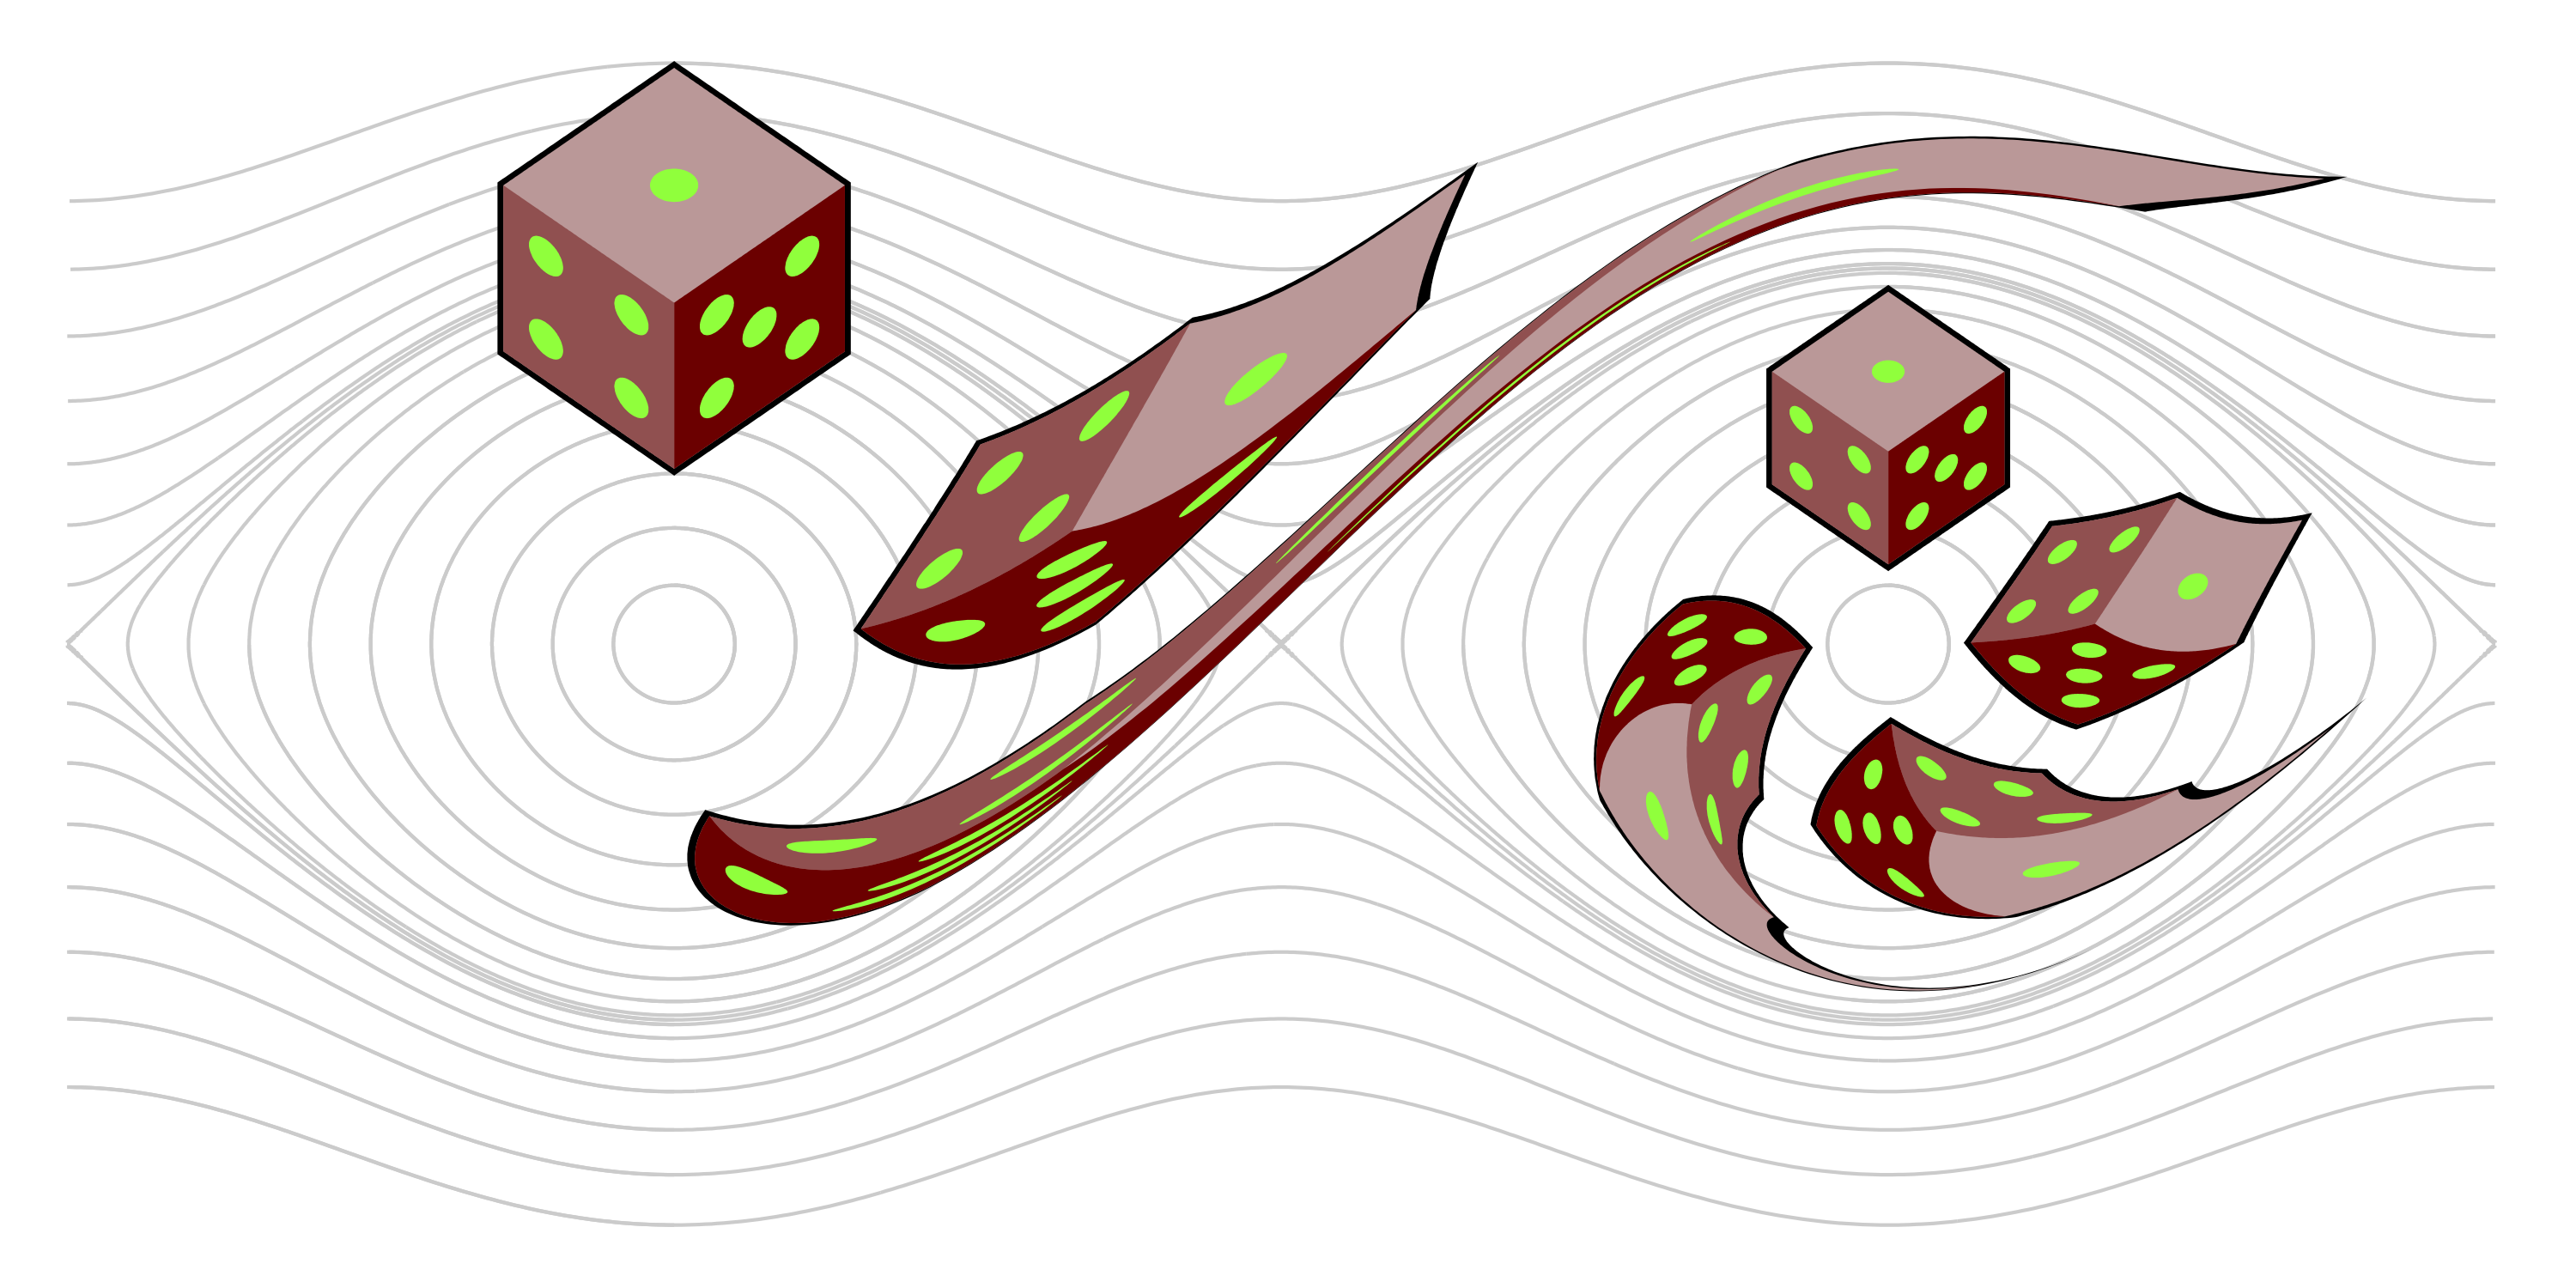
\includegraphics{figures/flow.png}

}

\subcaption{\label{fig-flow}}

\end{minipage}%

\caption{\label{fig-logo-motivation}(a) The logo for my consulting and
training company, Symplectomorphic, is a warped die (b) that was
generated by transforming an imagine of a square die with a
symplectomorphic transformation.}

\end{figure}%

\begin{figure}

\centering{

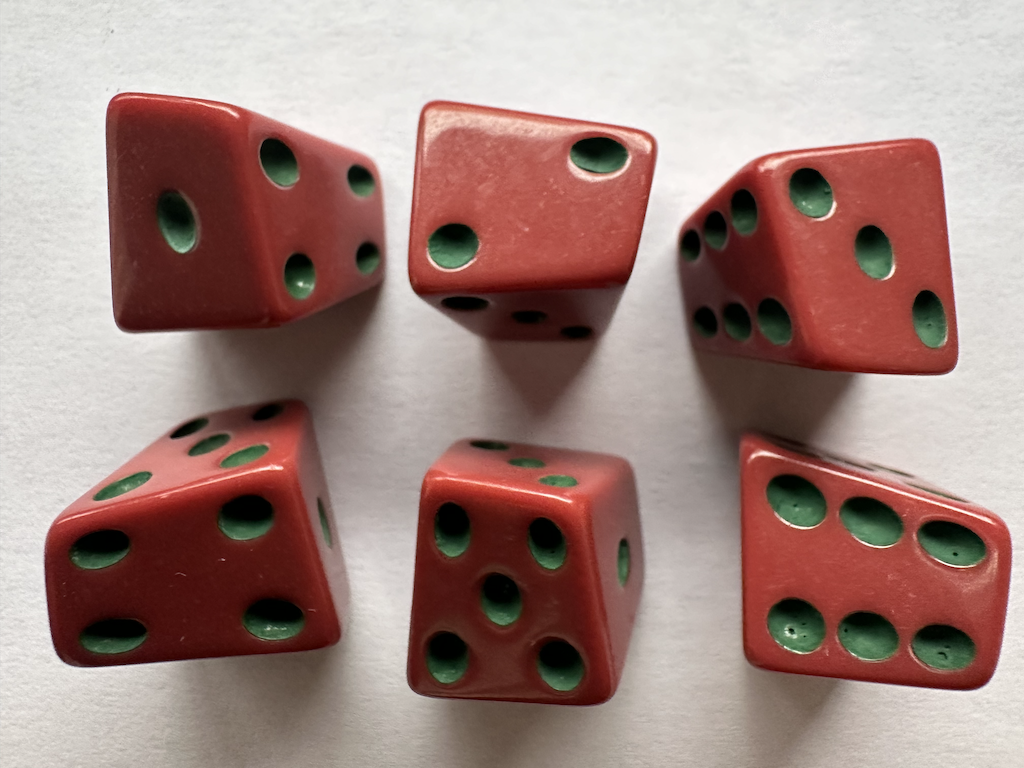
\includegraphics[width=0.75\textwidth,height=\textheight]{figures/dice.png}

}

\caption{\label{fig-warped-dice}Because we live in the future one can
actually exchange money for warped six-sided dice in custom colors.
Although the shape of these dice doesn't exactly match the warping of a
symplectomorphism it's about as close as one can get without contracting
a factory directly.}

\end{figure}%

At a workshop in January 2023 I was giving away some dice to
participants when one Will Pierce has the \emph{audacity} to question
the integrity of the Skew Dice™. Once I had calmed down I realized that
this challenge raised an interesting question: how exactly can we learn
how fair a die is in practice?

The
\href{https://www.mathartfun.com/thedicelab.com/DiceDesign.html}{Dice
Lab website} provides a geometric argument for why the Skew Dice™ should
roll fairly:

\begin{quote}
Skew Dice™ are based on the trigonal trapezohedron. (A cube is a special
case of a trigonal trapezohedron.) We distorted the faces in such a way
that they remained flat and are congruent (each one has the same size
and shape). In addition, the distorted polyhedron is an isohedron,
meaning that the symmetry group of the polyhedron is transitive on the
faces. Despite their bizarre appearance, this means that Skew Dice are
just as fair as regular dice.
\end{quote}

This argument, however, assumes that each die is manufactured precisely
and with uniform material density. Without being able to test these
mechanical properties directly all we can do is roll the dice over and
over again and investigate how often each side lands facing upwards.

In this case study I present a series of Bayesian analyses that attempt
to infer just how fair the Skew Dice™ that I ordered might be using
hundreds of physical die rolls performed by a small group of volunteers.
Along the way I'll present various techniques for working with
categorical data and simplex model configurations, including some
approaches for incorporation heterogeneity.

\section{Data Exploration}\label{data-exploration}

To ensure as rich of a data set as possible I sent Skew Dice™ to Adriano
Yoshino, EM Wolkovich, Joe Wozny, Karim Naguib, Ian Costley, and John
Flournoy, six of my generous
\href{https://www.patreon.com/betanalpha}{Patreon} supporters who
volunteered their own, and in some cases their friends' and family's,
time. Each volunteer then collected data from repeated rolls, recording
which die was thrown, who threw it, and what the outcome was. Once all
of the data had been shared I collected it into a single \texttt{R} data
frame with unique indices for each die and player.

\begin{Shaded}
\begin{Highlighting}[]
\FunctionTok{par}\NormalTok{(}\AttributeTok{family=}\StringTok{"serif"}\NormalTok{, }\AttributeTok{las=}\DecValTok{1}\NormalTok{, }\AttributeTok{bty=}\StringTok{"l"}\NormalTok{,}
    \AttributeTok{cex.axis=}\DecValTok{1}\NormalTok{, }\AttributeTok{cex.lab=}\DecValTok{1}\NormalTok{, }\AttributeTok{cex.main=}\DecValTok{1}\NormalTok{,}
    \AttributeTok{xaxs=}\StringTok{"i"}\NormalTok{, }\AttributeTok{yaxs=}\StringTok{"i"}\NormalTok{, }\AttributeTok{mar =} \FunctionTok{c}\NormalTok{(}\DecValTok{5}\NormalTok{, }\DecValTok{5}\NormalTok{, }\DecValTok{3}\NormalTok{, }\DecValTok{5}\NormalTok{))}
\end{Highlighting}
\end{Shaded}

\begin{Shaded}
\begin{Highlighting}[]
\NormalTok{df }\OtherTok{\textless{}{-}} \FunctionTok{read.csv}\NormalTok{(}\StringTok{"data/rolls.csv"}\NormalTok{)}


\NormalTok{N }\OtherTok{\textless{}{-}} \FunctionTok{nrow}\NormalTok{(df)}
\NormalTok{N\_players }\OtherTok{\textless{}{-}} \FunctionTok{length}\NormalTok{(}\FunctionTok{unique}\NormalTok{(df}\SpecialCharTok{$}\NormalTok{player\_idxs))}
\NormalTok{N\_dice }\OtherTok{\textless{}{-}} \FunctionTok{length}\NormalTok{(}\FunctionTok{unique}\NormalTok{(df}\SpecialCharTok{$}\NormalTok{die\_idxs))}

\NormalTok{data }\OtherTok{\textless{}{-}} \FunctionTok{list}\NormalTok{(}\StringTok{"N"} \OtherTok{=}\NormalTok{ N,}
             \StringTok{"outcome"} \OtherTok{=}\NormalTok{ df}\SpecialCharTok{$}\NormalTok{outcome,}
             \StringTok{"N\_players"} \OtherTok{=}\NormalTok{ N\_players,}
             \StringTok{"player\_idxs"} \OtherTok{=}\NormalTok{ df}\SpecialCharTok{$}\NormalTok{player\_idxs,}
             \StringTok{"N\_dice"} \OtherTok{=}\NormalTok{ N\_dice,}
             \StringTok{"die\_idxs"} \OtherTok{=}\NormalTok{ df}\SpecialCharTok{$}\NormalTok{die\_idxs)}
\end{Highlighting}
\end{Shaded}

Altogether 10 unique individuals used a combination of 12 unique dice to
give a 1682 total rolls.

\begin{Shaded}
\begin{Highlighting}[]
\FunctionTok{print}\NormalTok{(}\FunctionTok{sprintf}\NormalTok{(}\StringTok{"\%s total rolls"}\NormalTok{, N))}
\end{Highlighting}
\end{Shaded}

\begin{verbatim}
[1] "1682 total rolls"
\end{verbatim}

\begin{Shaded}
\begin{Highlighting}[]
\FunctionTok{print}\NormalTok{(}\FunctionTok{sprintf}\NormalTok{(}\StringTok{"\%s distinct players"}\NormalTok{, N\_players))}
\end{Highlighting}
\end{Shaded}

\begin{verbatim}
[1] "10 distinct players"
\end{verbatim}

\begin{Shaded}
\begin{Highlighting}[]
\FunctionTok{print}\NormalTok{(}\FunctionTok{sprintf}\NormalTok{(}\StringTok{"\%s distinct dice"}\NormalTok{, N\_dice))}
\end{Highlighting}
\end{Shaded}

\begin{verbatim}
[1] "12 distinct dice"
\end{verbatim}

Because each individual had access to only a few dice, however, the data
include only a few player-dice pairings.

\begin{Shaded}
\begin{Highlighting}[]
\FunctionTok{par}\NormalTok{(}\AttributeTok{mfrow=}\FunctionTok{c}\NormalTok{(}\DecValTok{1}\NormalTok{, }\DecValTok{1}\NormalTok{), }\AttributeTok{mar=}\FunctionTok{c}\NormalTok{(}\DecValTok{5}\NormalTok{, }\DecValTok{5}\NormalTok{, }\DecValTok{1}\NormalTok{, }\DecValTok{1}\NormalTok{))}

\FunctionTok{library}\NormalTok{(colormap)}
\NormalTok{disc\_colors }\OtherTok{\textless{}{-}} \FunctionTok{c}\NormalTok{(}\StringTok{"\#FFFFFF"}\NormalTok{, }\StringTok{"\#DCBCBC"}\NormalTok{, }\StringTok{"\#C79999"}\NormalTok{, }\StringTok{"\#B97C7C"}\NormalTok{,}
                 \StringTok{"\#A25050"}\NormalTok{, }\StringTok{"\#8F2727"}\NormalTok{, }\StringTok{"\#7C0000"}\NormalTok{)}
\NormalTok{cont\_colors }\OtherTok{\textless{}{-}} \FunctionTok{colormap}\NormalTok{(}\AttributeTok{colormap=}\NormalTok{disc\_colors, }\AttributeTok{nshades=}\DecValTok{100}\NormalTok{)}

\NormalTok{zs }\OtherTok{\textless{}{-}} \FunctionTok{table}\NormalTok{(data}\SpecialCharTok{$}\NormalTok{player\_idxs, data}\SpecialCharTok{$}\NormalTok{die\_idxs)}

\FunctionTok{image}\NormalTok{(}\DecValTok{1}\SpecialCharTok{:}\NormalTok{N\_players, }\DecValTok{1}\SpecialCharTok{:}\NormalTok{N\_dice, zs,}
      \AttributeTok{col=}\FunctionTok{rev}\NormalTok{(cont\_colors),}
      \AttributeTok{xlab=}\StringTok{"Player Index"}\NormalTok{, }\AttributeTok{ylab=}\StringTok{"Die Index"}\NormalTok{)}

\ControlFlowTok{for}\NormalTok{ (d }\ControlFlowTok{in} \DecValTok{1}\SpecialCharTok{:}\NormalTok{N\_dice) }\FunctionTok{abline}\NormalTok{(}\AttributeTok{h=}\NormalTok{d }\SpecialCharTok{{-}} \FloatTok{0.5}\NormalTok{, }\AttributeTok{lwd=}\FloatTok{1.5}\NormalTok{, }\AttributeTok{col=}\StringTok{"white"}\NormalTok{)}
\ControlFlowTok{for}\NormalTok{ (p }\ControlFlowTok{in} \DecValTok{1}\SpecialCharTok{:}\NormalTok{N\_players) }\ControlFlowTok{for}\NormalTok{ (d }\ControlFlowTok{in} \DecValTok{1}\SpecialCharTok{:}\NormalTok{N\_dice) }\FunctionTok{text}\NormalTok{(p, d, zs[p, d], }\AttributeTok{col=}\StringTok{"white"}\NormalTok{)}
\end{Highlighting}
\end{Shaded}

\includegraphics{die_fairness_files/figure-pdf/unnamed-chunk-5-1.pdf}

The rolls themselves appear to be reasonably uniform across the six
faces, both in aggregate and individually for each die.

\begin{Shaded}
\begin{Highlighting}[]
\NormalTok{util }\OtherTok{\textless{}{-}} \FunctionTok{new.env}\NormalTok{()}
\FunctionTok{source}\NormalTok{(}\StringTok{\textquotesingle{}mcmc\_visualization\_tools.R\textquotesingle{}}\NormalTok{, }\AttributeTok{local=}\NormalTok{util)}
\end{Highlighting}
\end{Shaded}

\begin{Shaded}
\begin{Highlighting}[]
\FunctionTok{par}\NormalTok{(}\AttributeTok{mfrow=}\FunctionTok{c}\NormalTok{(}\DecValTok{1}\NormalTok{, }\DecValTok{1}\NormalTok{), }\AttributeTok{mar=}\FunctionTok{c}\NormalTok{(}\DecValTok{5}\NormalTok{, }\DecValTok{5}\NormalTok{, }\DecValTok{3}\NormalTok{, }\DecValTok{1}\NormalTok{))}

\NormalTok{util}\SpecialCharTok{$}\FunctionTok{plot\_line\_hist}\NormalTok{(data}\SpecialCharTok{$}\NormalTok{outcome, }\FloatTok{0.5}\NormalTok{, }\FloatTok{6.5}\NormalTok{, }\DecValTok{1}\NormalTok{,}
                    \AttributeTok{xlab=}\StringTok{"Face"}\NormalTok{, }\AttributeTok{main=}\StringTok{"All Rolls"}\NormalTok{)}
\FunctionTok{abline}\NormalTok{(}\AttributeTok{h=}\NormalTok{data}\SpecialCharTok{$}\NormalTok{N }\SpecialCharTok{/} \DecValTok{6}\NormalTok{, }\AttributeTok{lty=}\DecValTok{2}\NormalTok{, }\AttributeTok{lwd=}\DecValTok{3}\NormalTok{, }\AttributeTok{col=}\StringTok{"\#DDDDDD"}\NormalTok{)}
\end{Highlighting}
\end{Shaded}

\includegraphics{die_fairness_files/figure-pdf/unnamed-chunk-7-1.pdf}

\begin{Shaded}
\begin{Highlighting}[]
\ControlFlowTok{for}\NormalTok{ (d }\ControlFlowTok{in} \DecValTok{1}\SpecialCharTok{:}\NormalTok{data}\SpecialCharTok{$}\NormalTok{N\_dice) \{}
  \ControlFlowTok{if}\NormalTok{ (d }\SpecialCharTok{\%\%} \DecValTok{6} \SpecialCharTok{==} \DecValTok{1}\NormalTok{) }\FunctionTok{par}\NormalTok{(}\AttributeTok{mfrow=}\FunctionTok{c}\NormalTok{(}\DecValTok{2}\NormalTok{, }\DecValTok{3}\NormalTok{), }\AttributeTok{mar=}\FunctionTok{c}\NormalTok{(}\DecValTok{4}\NormalTok{, }\DecValTok{5}\NormalTok{, }\DecValTok{2}\NormalTok{, }\DecValTok{1}\NormalTok{))}

\NormalTok{  util}\SpecialCharTok{$}\FunctionTok{plot\_line\_hist}\NormalTok{(data}\SpecialCharTok{$}\NormalTok{outcome[data}\SpecialCharTok{$}\NormalTok{die\_idxs }\SpecialCharTok{==}\NormalTok{ d],}
                 \FloatTok{0.5}\NormalTok{, }\FloatTok{6.5}\NormalTok{, }\DecValTok{1}\NormalTok{, }\AttributeTok{xlab=}\StringTok{"Face"}\NormalTok{, }\AttributeTok{main=}\FunctionTok{paste}\NormalTok{(}\StringTok{"Die"}\NormalTok{, d))}
  \FunctionTok{abline}\NormalTok{(}\AttributeTok{h=}\FunctionTok{sum}\NormalTok{(data}\SpecialCharTok{$}\NormalTok{die\_idxs }\SpecialCharTok{==}\NormalTok{ d) }\SpecialCharTok{/} \DecValTok{6}\NormalTok{, }\AttributeTok{lty=}\DecValTok{2}\NormalTok{, }\AttributeTok{lwd=}\DecValTok{3}\NormalTok{, }\AttributeTok{col=}\StringTok{"\#DDDDDD"}\NormalTok{)}
\NormalTok{\}}
\end{Highlighting}
\end{Shaded}

\includegraphics{die_fairness_files/figure-pdf/unnamed-chunk-8-1.pdf}

\includegraphics{die_fairness_files/figure-pdf/unnamed-chunk-8-2.pdf}

That said the recorded outcomes are not \emph{exactly} uniform. Our
statistical challenge is to determine just how large the deviations from
exact uniformity need to be before we need to be concerned about unfair
dice.

\section{Uniform Simplex Model}\label{uniform-simplex-model}

If we assume that the outcome of rolling a die is unpredictable then we
won't expect exactly uniform outcomes, even when a die is fair. In order
to quantify these deviations we need to build a predictive model.

\subsection{The Observational Model}\label{the-observational-model}

Each roll of a die on a flat surface results in one, and only one, face.
If we label each face with one of six integers then the observational
space becomes \[
Y = \{ 1, 2, 3, 4, 5, 6 \}.
\]

In general we can model the relative frequencies of each these six
outcomes with a finite probability distribution specified by six atomic
probabilities, \begin{align*}
\pi( \{ 1 \} ) &= q_{1}
\\
\ldots&
\\
\pi( \{ k \} ) &= q_{k}
\\
\ldots&
\\
\pi( \{ 6 \} ) &= q_{6}
\end{align*} satisfying the constraints \[
0 \le q_{k} \le 1
\] and \[
\sum_{k = 1}^{6} q_{k} = 1.
\] The observational model for a single outcome is then given by
categorical distribution, \begin{align*}
p(y \mid q)
&=
\text{categorical}(y \mid q_{1}, \ldots, q_{k}, \ldots, q_{6})
\\
&\equiv
q_{k = y}.
\end{align*}

The space of all such probability distributions over six elements is
known as the \textbf{\(5\)-simplex} and is denoted \(\Delta^{5}\). Note
that we refer to this space as \(5\)-simplex and not a \(6\)-simplex
because the normalization constraint effectively remove one degree of
freedom. I will refer to any individual point in this simplex, \[
q = (q_{1}, \ldots, q_{k}, \ldots, q_{6}) \in \Delta^{5},
\] as a simplex configuration.

If the properties of a particular die do not change appreciably between
rolls then we should be able to model the outcome of multiple rolls
using the same simplex configuration. In this case the joint
observational model for multiple rolls reduces to a multinomial
distribution, \begin{align*}
p(y_{1}, \ldots, y_{N} \mid q_{1}, \ldots, q_{6})
&=
\prod_{n = 1}^{N}
\text{categorical}(y_{n} \mid q_{1}, \ldots, q_{6})
\\
&=
\prod_{n = 1}^{N} q_{k = y_{n}}
\\
&=
\prod_{k = 1}^{6}
q_{k}^{ \sum_{n = 1}^{N} \delta_{y_{n}, k} }
\\
&=
\prod_{k = 1}^{6} q_{k}^{ n_{k} },
\end{align*} where \(\delta_{y_{n}, k}\) is the Kronecker delta, \[
\delta_{y_{n}, k}
=
\left\{
\begin{array}{rr}
1, & y_{n} = k \\
0, & y_{n} \neq k
\end{array}
\right. ,
\] and \[
n_{k} = \sum_{n = 1}^{N} \delta_{y_{n}, k}
\] is the total number of rolls resulting in the \(k\)th face.

Finally if we assume that all of the dice behave identically then we can
model all of their outcomes with a multinomial distribution and a single
simplex configuration.

The context of this model provides a new way of interpreting
``fairness''. Instead of requiring that a fair die produce uniform
outcomes we can require that a fair die be modeled by the uniform
simplex configuration \[
\upsilon
=
\left( \frac{1}{6}, \frac{1}{6}, \frac{1}{6},
       \frac{1}{6}, \frac{1}{6}, \frac{1}{6}, \right) \in \Delta^{5}.
\] Interestingly this strict modeling assumption leaves us with no
degrees of freedom to infer from the data. Instead we can immediately
move on to the simulation of predictive data.

\subsection{Summary Statistics For Retrodictive
Checks}\label{summary-statistics-for-retrodictive-checks}

The observational space for all \(N = 1682\) rolls in our data set, \[
y_{1}, \ldots, y_{n}, \ldots, y_{N},
\] is \(1682\) dimensional. Unfortunately there are just a few too many
dimensions to be able to visualize a predictive distribution directly.

In order to construct productive retrodictive checks to critique this
model we'll need summary statistics that can reduce the
\(1682\)-dimensional observational space into something a bit more
manageable without sacrificing interpretability.

For example a histogram of the observed outcomes counts, \[
n_{1}, \ldots, n_{6}
\] is particularly natural for categorical data like this.

Moreover we can summarize the uniformity of these histograms using an
empirical entropy function over the individual counts \begin{align*}
\hat{H}(n_{1}, \ldots, n_{6})
&=
- \sum_{k = 1}^{6} \hat{q}_{k} \log \hat{q}_{k}
\\
&=
- \sum_{k = 1}^{6}
\left( \frac{n_{k}}{N} \right) \log \left( \frac{n_{k}}{N} \right).
\end{align*} The empirical entropy function is maximized when the
observed counts are exactly uniform, \[
n_{1} = \ldots = n_{6} = \frac{N}{6},
\] and minimized when we observe one and only one outcome \(k'\), \[
n_{k'} = N, n_{k \ne k'} = 0.
\] In a retrodictive check the empirical entropy allows us to
investigate how well our model captures the uniformity, or lack thereof,
exhibited by the observed rolls.

\subsection{Implementation}\label{implementation}

Because there are no free parameters we can simulate predictive data
directly in the \texttt{generated\ quantities} block of a Stan program.

\begin{codelisting}

\caption{\texttt{uniform\textbackslash\_simplex.stan}}

\begin{Shaded}
\begin{Highlighting}[]
\KeywordTok{data}\NormalTok{ \{}
  \DataTypeTok{int}\NormalTok{\textless{}}\KeywordTok{lower}\NormalTok{=}\DecValTok{1}\NormalTok{\textgreater{} N; }\CommentTok{// Number of rolls}
\NormalTok{\}}

\KeywordTok{transformed data}\NormalTok{ \{}
  \CommentTok{// Uniform simplex configuration}
  \DataTypeTok{simplex}\NormalTok{[}\DecValTok{6}\NormalTok{] upsilon = rep\_vector(}\FloatTok{1.0}\NormalTok{ / }\DecValTok{6}\NormalTok{, }\DecValTok{6}\NormalTok{);}
\NormalTok{\}}

\KeywordTok{generated quantities}\NormalTok{ \{}
  \CommentTok{// Compute predictions}
  \DataTypeTok{array}\NormalTok{[}\DecValTok{6}\NormalTok{] }\DataTypeTok{int}\NormalTok{ pred\_counts = multinomial\_rng(upsilon, N);}
  \DataTypeTok{real}\NormalTok{ pred\_entropy = }\DecValTok{0}\NormalTok{;}
  \ControlFlowTok{for}\NormalTok{ (k }\ControlFlowTok{in} \DecValTok{1}\NormalTok{:}\DecValTok{6}\NormalTok{) \{}
    \DataTypeTok{real}\NormalTok{ q\_hat = pred\_counts[k] * }\FloatTok{1.0}\NormalTok{ / N;}
\NormalTok{    pred\_entropy += {-} lmultiply(q\_hat, q\_hat);}
\NormalTok{  \}}
\NormalTok{\}}
\end{Highlighting}
\end{Shaded}

\end{codelisting}

The \texttt{Fixed\_param} algorithm in \texttt{RStan} then allows us to
repeatedly evaluate this \texttt{generated\ quantities} block to
generate an ensemble of predictive summary statistic outputs.

\begin{Shaded}
\begin{Highlighting}[]
\FunctionTok{library}\NormalTok{(rstan)}
\FunctionTok{rstan\_options}\NormalTok{(}\AttributeTok{auto\_write =} \ConstantTok{TRUE}\NormalTok{)            }\CommentTok{\# Cache compiled Stan programs}
\FunctionTok{options}\NormalTok{(}\AttributeTok{mc.cores =}\NormalTok{ parallel}\SpecialCharTok{::}\FunctionTok{detectCores}\NormalTok{()) }\CommentTok{\# Parallelize chains}
\NormalTok{parallel}\SpecialCharTok{:::}\FunctionTok{setDefaultClusterOptions}\NormalTok{(}\AttributeTok{setup\_strategy =} \StringTok{"sequential"}\NormalTok{)}

\FunctionTok{source}\NormalTok{(}\StringTok{\textquotesingle{}mcmc\_analysis\_tools\_rstan.R\textquotesingle{}}\NormalTok{, }\AttributeTok{local=}\NormalTok{util)}
\end{Highlighting}
\end{Shaded}

\begin{Shaded}
\begin{Highlighting}[]
\NormalTok{fit }\OtherTok{\textless{}{-}} \FunctionTok{stan}\NormalTok{(}\AttributeTok{file=}\StringTok{"stan\_programs/uniform\_simplex.stan"}\NormalTok{,}
            \AttributeTok{algorithm=}\StringTok{"Fixed\_param"}\NormalTok{, }\AttributeTok{data=}\NormalTok{data, }\AttributeTok{seed=}\DecValTok{8438338}\NormalTok{,}
            \AttributeTok{warmup=}\DecValTok{1000}\NormalTok{, }\AttributeTok{iter=}\DecValTok{2024}\NormalTok{, }\AttributeTok{refresh=}\DecValTok{0}\NormalTok{)}

\NormalTok{samples }\OtherTok{\textless{}{-}}\NormalTok{ util}\SpecialCharTok{$}\FunctionTok{extract\_expectands}\NormalTok{(fit)}
\end{Highlighting}
\end{Shaded}

As we're not running Markov chain Monte Carlo here there are no
computational diagnostics to consider and we can instead jump straight
into the retrodictive checks.

Let's first consider the retrodictive behavior within each histogram
bin, comparing each observed count to the corresponding predictive
count.

\begin{Shaded}
\begin{Highlighting}[]
\FunctionTok{par}\NormalTok{(}\AttributeTok{mfrow=}\FunctionTok{c}\NormalTok{(}\DecValTok{2}\NormalTok{, }\DecValTok{3}\NormalTok{), }\AttributeTok{mar=}\FunctionTok{c}\NormalTok{(}\DecValTok{5}\NormalTok{, }\DecValTok{5}\NormalTok{, }\DecValTok{3}\NormalTok{, }\DecValTok{1}\NormalTok{))}

\NormalTok{obs\_counts }\OtherTok{\textless{}{-}} \FunctionTok{table}\NormalTok{(data}\SpecialCharTok{$}\NormalTok{outcome)}

\ControlFlowTok{for}\NormalTok{ (k }\ControlFlowTok{in} \DecValTok{1}\SpecialCharTok{:}\DecValTok{6}\NormalTok{) \{}
\NormalTok{  name }\OtherTok{\textless{}{-}} \FunctionTok{paste0}\NormalTok{(}\StringTok{\textquotesingle{}pred\_counts[\textquotesingle{}}\NormalTok{, k, }\StringTok{\textquotesingle{}]\textquotesingle{}}\NormalTok{)}
\NormalTok{  util}\SpecialCharTok{$}\FunctionTok{plot\_expectand\_pushforward}\NormalTok{(samples[[name]], }\DecValTok{20}\NormalTok{,}
                                  \AttributeTok{display\_name=}\StringTok{"Counts"}\NormalTok{,}
                                  \AttributeTok{main=}\FunctionTok{paste0}\NormalTok{(}\StringTok{"Face "}\NormalTok{, k),}
                                  \AttributeTok{baseline=}\NormalTok{obs\_counts[k])}
\NormalTok{\}}
\end{Highlighting}
\end{Shaded}

\includegraphics{die_fairness_files/figure-pdf/unnamed-chunk-11-1.pdf}

Overall there don't appear to be any serious retrodictive disagreements.
That said there are a few outcomes for which the observed counts fall
into the tails of the corresponding predictive distribution.

In order to investigate for any patterns in these mild retrodictive
tensions it will help to visualizing the observed and predictive
behaviors for all outcomes at the same time. One particularly convenient
way to do this is with nested quantile intervals.

\begin{Shaded}
\begin{Highlighting}[]
\FunctionTok{par}\NormalTok{(}\AttributeTok{mfrow=}\FunctionTok{c}\NormalTok{(}\DecValTok{1}\NormalTok{, }\DecValTok{1}\NormalTok{), }\AttributeTok{mar=}\FunctionTok{c}\NormalTok{(}\DecValTok{5}\NormalTok{, }\DecValTok{5}\NormalTok{, }\DecValTok{3}\NormalTok{, }\DecValTok{1}\NormalTok{))}

\NormalTok{obs\_counts }\OtherTok{\textless{}{-}} \FunctionTok{table}\NormalTok{(data}\SpecialCharTok{$}\NormalTok{outcome)}

\NormalTok{pred\_names }\OtherTok{\textless{}{-}} \FunctionTok{sapply}\NormalTok{(}\DecValTok{1}\SpecialCharTok{:}\DecValTok{6}\NormalTok{, }\ControlFlowTok{function}\NormalTok{(k) }\FunctionTok{paste0}\NormalTok{(}\StringTok{\textquotesingle{}pred\_counts[\textquotesingle{}}\NormalTok{, k, }\StringTok{\textquotesingle{}]\textquotesingle{}}\NormalTok{))}
\NormalTok{util}\SpecialCharTok{$}\FunctionTok{plot\_disc\_pushforward\_quantiles}\NormalTok{(samples, pred\_names,}
                                     \AttributeTok{baseline\_values=}\NormalTok{obs\_counts,}
                                     \AttributeTok{xlab=}\StringTok{"Face"}\NormalTok{, }\AttributeTok{display\_ylim=}\FunctionTok{c}\NormalTok{(}\DecValTok{225}\NormalTok{, }\DecValTok{325}\NormalTok{))}
\end{Highlighting}
\end{Shaded}

\includegraphics{die_fairness_files/figure-pdf/unnamed-chunk-12-1.pdf}

Immediately we see that the observed counts aren't completely contained
within the predictive quantile intervals. That, however, is not
necessarily surprising. For example the largest intervals shown here
span only the 10\% to 90\% predictive quantiles; 10\% predictive
probability continues below the lightest band and 10\% continues above
it. At the same time because the marginal quantiles are not sensitive to
correlations in the counts they tend to underestimate the joint
variation.

The empirical entropy retrodictive check, which directly quantifies the
deviation of the observed counts from exact uniformity, exhibits the
same mild retrodictive tension seen in the retrodictive checks for each
outcome. This at least qualitatively supports the adequacy of uniform
simplex model, and the fairness of the dice.

\begin{Shaded}
\begin{Highlighting}[]
\FunctionTok{par}\NormalTok{(}\AttributeTok{mfrow=}\FunctionTok{c}\NormalTok{(}\DecValTok{1}\NormalTok{, }\DecValTok{1}\NormalTok{))}

\NormalTok{obs\_entropy }\OtherTok{\textless{}{-}} \FunctionTok{sum}\NormalTok{(}\FunctionTok{sapply}\NormalTok{(obs\_counts,}
                          \ControlFlowTok{function}\NormalTok{(n) }\SpecialCharTok{{-}}\NormalTok{(n }\SpecialCharTok{/}\NormalTok{ data}\SpecialCharTok{$}\NormalTok{N) }\SpecialCharTok{*} \FunctionTok{log}\NormalTok{(n }\SpecialCharTok{/}\NormalTok{ data}\SpecialCharTok{$}\NormalTok{N)))}

\NormalTok{util}\SpecialCharTok{$}\FunctionTok{plot\_expectand\_pushforward}\NormalTok{(samples[[}\StringTok{"pred\_entropy"}\NormalTok{]], }\DecValTok{20}\NormalTok{,}
                                \AttributeTok{display\_name=}\StringTok{"Empirical Entropy"}\NormalTok{,}
                                \AttributeTok{baseline=}\NormalTok{obs\_entropy)}
\end{Highlighting}
\end{Shaded}

\includegraphics{die_fairness_files/figure-pdf/unnamed-chunk-13-1.pdf}

\subsection{Interpreting the Possible Retrodictive
Tension}\label{interpreting-the-possible-retrodictive-tension}

The shape of the mild retrodictive tension in the histogram summary
statistic is useful for motivating possible model inadequacies, and
hence productive model expansions. Here the tension suggests that the
uniform simplex model might be underestimating the occurrence of faces 3
and 4 while overestimating the occurrence of faces 1 and 6.

One advantage of knowing the provenance of the data is that we can
compare this behavior to our domain expertise. In particular we can
consider whether or not this deviation from uniformity is physically
reasonable.

The faces on each Skew Dice™ are arranged so that opposite faces always
sum to 7: 1 is opposite 6, 2 is opposite 5, and 3 is opposite 4. A
symmetric deficit of 1 and 6 rolls could be explained by less material
on these opposite faces relative to faces 2, 3, 4, and 5. Similarly a
symmetric excess of 3 and 4 rolls could be explained by an excess of
material on those opposite faces.

That said not every source of non-uniformity is consistent with these
patterns. For example biases caused by the asymmetric filling of a die
mold from one side to the other would manifest in excesses and deficits
that are similar between not \emph{opposite} faces but rather
\emph{neighboring} faces. Without knowing more details about the
manufacturing process, however, we can really only speculate.

\section{General Simplex Model}\label{general-simplex-model}

One way to clarify the situation is to consider a more elaborate model
and see if the added flexibility resolves any of the mild retrodictive
tension exhibited by the simpler model. If we can't find any beneficial
expansions then we can always return to the simpler model.

In this section we'll consider a model that takes advantage of the
entire simplex \(\Delta^{5}\). We will continue to assume that the dice
behave identically so that all of the data can be modeled with a single
multinomial distribution.

\subsection{Inferences}\label{inferences}

Conveniently modeling general simplex configurations is straightforward
in Stan due to the \texttt{simplex} variable type which automatically
enforces the simplex constraints. With only limited information about
the manufacturing of the dice we'll use a uniform prior density function
over the entire simplex.

\begin{codelisting}

\caption{\texttt{homogeneous\textbackslash\_simplex.stan}}

\begin{Shaded}
\begin{Highlighting}[]
\KeywordTok{data}\NormalTok{ \{}
  \DataTypeTok{int}\NormalTok{\textless{}}\KeywordTok{lower}\NormalTok{=}\DecValTok{1}\NormalTok{\textgreater{} N;                         }\CommentTok{// Number of rolls}
  \DataTypeTok{array}\NormalTok{[N] }\DataTypeTok{int}\NormalTok{\textless{}}\KeywordTok{lower}\NormalTok{=}\DecValTok{1}\NormalTok{, }\KeywordTok{upper}\NormalTok{=}\DecValTok{6}\NormalTok{\textgreater{} outcome; }\CommentTok{// Roll outcomes}
\NormalTok{\}}

\KeywordTok{transformed data}\NormalTok{ \{}
  \CommentTok{// Compute outcome totals}
  \DataTypeTok{array}\NormalTok{[}\DecValTok{6}\NormalTok{] }\DataTypeTok{int}\NormalTok{ counts = rep\_array(}\DecValTok{0}\NormalTok{, }\DecValTok{6}\NormalTok{);}
  \ControlFlowTok{for}\NormalTok{ (n }\ControlFlowTok{in} \DecValTok{1}\NormalTok{:N) \{}
\NormalTok{    counts[outcome[n]] += }\DecValTok{1}\NormalTok{;}
\NormalTok{  \}}
\NormalTok{\}}

\KeywordTok{parameters}\NormalTok{ \{}
  \CommentTok{// General simplex configuration}
  \DataTypeTok{simplex}\NormalTok{[}\DecValTok{6}\NormalTok{] q;}
\NormalTok{\}}

\KeywordTok{model}\NormalTok{ \{}
\NormalTok{  q \textasciitilde{} dirichlet(rep\_vector(}\DecValTok{1}\NormalTok{, }\DecValTok{6}\NormalTok{));}
\NormalTok{  counts \textasciitilde{} multinomial(q);}
\NormalTok{\}}

\KeywordTok{generated quantities}\NormalTok{ \{}
  \CommentTok{// Posterior predictions}
  \DataTypeTok{array}\NormalTok{[}\DecValTok{6}\NormalTok{] }\DataTypeTok{int}\NormalTok{ pred\_counts = multinomial\_rng(q, N);}
  \DataTypeTok{real}\NormalTok{ pred\_entropy = }\DecValTok{0}\NormalTok{;}

  \ControlFlowTok{for}\NormalTok{ (k }\ControlFlowTok{in} \DecValTok{1}\NormalTok{:}\DecValTok{6}\NormalTok{) \{}
    \DataTypeTok{real}\NormalTok{ q\_hat = pred\_counts[k] * }\FloatTok{1.0}\NormalTok{ / N;}
\NormalTok{    pred\_entropy += {-} lmultiply(q\_hat, q\_hat);}
\NormalTok{  \}}
\NormalTok{\}}
\end{Highlighting}
\end{Shaded}

\end{codelisting}

\begin{Shaded}
\begin{Highlighting}[]
\NormalTok{fit }\OtherTok{\textless{}{-}} \FunctionTok{stan}\NormalTok{(}\AttributeTok{file=}\StringTok{"stan\_programs/homogeneous\_simplex.stan"}\NormalTok{,}
            \AttributeTok{data=}\NormalTok{data, }\AttributeTok{seed=}\DecValTok{8438338}\NormalTok{,}
            \AttributeTok{warmup=}\DecValTok{1000}\NormalTok{, }\AttributeTok{iter=}\DecValTok{2024}\NormalTok{, }\AttributeTok{refresh=}\DecValTok{0}\NormalTok{)}
\end{Highlighting}
\end{Shaded}

The diagnostics don't suggest that Stan's Hamiltonian Monte Carlo
sampler is encountering any problems in its efforts to quantifying the
posterior distribution.

\begin{Shaded}
\begin{Highlighting}[]
\NormalTok{diagnostics }\OtherTok{\textless{}{-}}\NormalTok{ util}\SpecialCharTok{$}\FunctionTok{extract\_hmc\_diagnostics}\NormalTok{(fit)}
\NormalTok{util}\SpecialCharTok{$}\FunctionTok{check\_all\_hmc\_diagnostics}\NormalTok{(diagnostics)}
\end{Highlighting}
\end{Shaded}

\begin{verbatim}
  All Hamiltonian Monte Carlo diagnostics are consistent with reliable
Markov chain Monte Carlo.
\end{verbatim}

\begin{Shaded}
\begin{Highlighting}[]
\NormalTok{samples }\OtherTok{\textless{}{-}}\NormalTok{ util}\SpecialCharTok{$}\FunctionTok{extract\_expectands}\NormalTok{(fit)}
\NormalTok{base\_samples }\OtherTok{\textless{}{-}}\NormalTok{ util}\SpecialCharTok{$}\FunctionTok{filter\_expectands}\NormalTok{(samples, }\StringTok{\textquotesingle{}q\textquotesingle{}}\NormalTok{, }\AttributeTok{check\_arrays=}\ConstantTok{TRUE}\NormalTok{)}
\NormalTok{util}\SpecialCharTok{$}\FunctionTok{check\_all\_expectand\_diagnostics}\NormalTok{(base\_samples)}
\end{Highlighting}
\end{Shaded}

\begin{verbatim}
All expectands checked appear to be behaving well enough for reliable
Markov chain Monte Carlo estimation.
\end{verbatim}

With an accurate posterior quantification we can faithfully compare the
posterior predictive distribution to the observed data. The general
simplex model appears to have more than enough flexibility to reproduce
all of the behaviors in the observed data that manifest in the total
outcome frequencies and empirical entropy.

\begin{Shaded}
\begin{Highlighting}[]
\FunctionTok{par}\NormalTok{(}\AttributeTok{mfrow=}\FunctionTok{c}\NormalTok{(}\DecValTok{1}\NormalTok{, }\DecValTok{1}\NormalTok{))}

\NormalTok{pred\_names }\OtherTok{\textless{}{-}} \FunctionTok{sapply}\NormalTok{(}\DecValTok{1}\SpecialCharTok{:}\DecValTok{6}\NormalTok{, }\ControlFlowTok{function}\NormalTok{(k) }\FunctionTok{paste0}\NormalTok{(}\StringTok{\textquotesingle{}pred\_counts[\textquotesingle{}}\NormalTok{, k, }\StringTok{\textquotesingle{}]\textquotesingle{}}\NormalTok{))}
\NormalTok{util}\SpecialCharTok{$}\FunctionTok{plot\_disc\_pushforward\_quantiles}\NormalTok{(samples, pred\_names,}
                                     \AttributeTok{baseline\_values=}\NormalTok{obs\_counts,}
                                     \AttributeTok{xlab=}\StringTok{"Outcome"}\NormalTok{, }\AttributeTok{ylab=}\StringTok{"Counts"}\NormalTok{)}
\end{Highlighting}
\end{Shaded}

\includegraphics{die_fairness_files/figure-pdf/unnamed-chunk-16-1.pdf}

\begin{Shaded}
\begin{Highlighting}[]
\FunctionTok{par}\NormalTok{(}\AttributeTok{mfrow=}\FunctionTok{c}\NormalTok{(}\DecValTok{1}\NormalTok{, }\DecValTok{1}\NormalTok{))}

\NormalTok{obs\_entropy }\OtherTok{\textless{}{-}} \FunctionTok{sum}\NormalTok{(}\FunctionTok{sapply}\NormalTok{(obs\_counts,}
                          \ControlFlowTok{function}\NormalTok{(n) }\SpecialCharTok{{-}}\NormalTok{(n }\SpecialCharTok{/}\NormalTok{ data}\SpecialCharTok{$}\NormalTok{N) }\SpecialCharTok{*} \FunctionTok{log}\NormalTok{(n }\SpecialCharTok{/}\NormalTok{ data}\SpecialCharTok{$}\NormalTok{N)))}

\NormalTok{util}\SpecialCharTok{$}\FunctionTok{plot\_expectand\_pushforward}\NormalTok{(samples[[}\StringTok{"pred\_entropy"}\NormalTok{]], }\DecValTok{20}\NormalTok{,}
                                \AttributeTok{display\_name=}\StringTok{"Empirical Entropy"}\NormalTok{,}
                                \AttributeTok{baseline=}\NormalTok{obs\_entropy)}
\end{Highlighting}
\end{Shaded}

\includegraphics{die_fairness_files/figure-pdf/unnamed-chunk-17-1.pdf}

Because there is no visible posterior retrodictive tension the posterior
inferences from this model should capture meaningful insights. In this
case the posterior distribution follows the pattern seen in the observed
counts, with an excess of probability for faces 3 and 4 and a deficit
for faces 1 and 6. That said the posterior distribution is not
concentrating all that far from the uniform simplex configuration.

\begin{Shaded}
\begin{Highlighting}[]
\NormalTok{names }\OtherTok{\textless{}{-}} \FunctionTok{sapply}\NormalTok{(}\DecValTok{1}\SpecialCharTok{:}\DecValTok{6}\NormalTok{, }\ControlFlowTok{function}\NormalTok{(k) }\FunctionTok{paste0}\NormalTok{(}\StringTok{\textquotesingle{}q[\textquotesingle{}}\NormalTok{, k, }\StringTok{\textquotesingle{}]\textquotesingle{}}\NormalTok{))}
\NormalTok{util}\SpecialCharTok{$}\FunctionTok{plot\_disc\_pushforward\_quantiles}\NormalTok{(samples, names,}
                                     \AttributeTok{xlab=}\StringTok{"Outcome"}\NormalTok{, }\AttributeTok{ylab=}\StringTok{"Probability"}\NormalTok{)}
\FunctionTok{abline}\NormalTok{(}\AttributeTok{h=}\DecValTok{1}\SpecialCharTok{/}\DecValTok{6}\NormalTok{, }\AttributeTok{col=}\StringTok{"\#DDDDDD"}\NormalTok{, }\AttributeTok{lwd=}\DecValTok{3}\NormalTok{, }\AttributeTok{lty=}\DecValTok{2}\NormalTok{)}
\end{Highlighting}
\end{Shaded}

\includegraphics{die_fairness_files/figure-pdf/unnamed-chunk-18-1.pdf}

\subsection{Decisions}\label{decisions}

Inferences from the general simplex model provide multiple ways to
characterize the fairness of the dice within the scope of the modeling
assumptions. In particular we can use our inferences to inform explicit
decisions about the fairness of the dice for each characterization. In
this section we'll see how we can use Bayesian decision theory to
construct systematic decisions.

\subsubsection{A Primer on Bayesian Decision
Theory}\label{a-primer-on-bayesian-decision-theory}

Formal decision making is defined by a space of actions, \(a \in A\),
and a utility function that numerically quantifies the overall benefits
of taking each action, \begin{alignat*}{6}
U :\; & A & &\rightarrow& \; & \mathbb{R} &
\\
& a & &\mapsto& & U(a) &.
\end{alignat*} Once we have defined a space of actions and a utility
function then the optimal decision is simply to take the action with the
highest utility, \[
a_{\mathrm{optimal}}
=
\underset{a \in A}{\mathrm{argmax}} \, \overline{U}(a).
\] Note that to simplify this discussion I am ignoring the possibility
of ties, but they are not difficult to accommodate by first identifying
the set of equally-optimal actions and then introducing a procedure to
arbitrarily choose from those actions.

For many problems the utility of each action will depend on unknown
behaviors. In these cases the best we can do is construct a model
configuration space of possible behaviors \(\Theta\) and then a
model-based utility function, \begin{alignat*}{6}
U :\; & A \times \Theta & &\rightarrow& \; & \mathbb{R} &
\\
& a, \theta & &\mapsto& & U(a, \theta) &.
\end{alignat*} Because the ordering of the actions by their assigned
utilities will in general vary with each model configuration \(\theta\),
\[
\underset{a \in A}{\mathrm{argmax}} \, \overline{U}(a, \theta)
\ne
\underset{a \in A}{\mathrm{argmax}} \, \overline{U}(a, \theta'),
\] there is no longer an unambiguous best action.

Bayesian decision theory uses posterior inferences to inform decision
making under exactly this sort of uncertainty. A posterior distribution
\(p(\theta \mid \tilde{y})\) informing the unknown behaviors defines
posterior expected utilities for each action, \[
\overline{U}(a \mid \tilde{y})
=
\int \mathrm{d} \theta \, p(\theta \mid \tilde{y}) , U(a, \theta).
\] Given the observation \(\tilde{y}\) the posterior expected utilities
depend on only the actions. Consequently we can use them to
unambiguously rank the actions and identify a single best action, \[
a_{\mathrm{optimal}}
=
\underset{a \in A}{\mathrm{argmax}} \, \overline{U}(a \mid \tilde{y}).
\] Again for simplicity I am ignoring the possibility of ties here.

\subsubsection{Fairness Actions}\label{sec:actions}

The space of actions that we consider in a decision making problem is
easy to take for granted. This is unfortunate because the worst
decisions often arise not from an inappropriate utility function but
rather from the restriction to an unnecessarily small space of actions,
all of which might be burdened with poor consequences.

When questioning the fairness of these dice there appear to be two
immediate actions that we can take:

\begin{itemize}
\tightlist
\item
  \(a_{1}\): declare that the dice are fair,
\item
  \(a_{2}\): declare that the dice are unfair.
\end{itemize}

In some applications a more refined set of actions might be more useful.
For example we could incorporate additional actions that avoid making
any declaration at all or even trigger followup data collection.

Even if these two actions are sufficient we still cannot move forwards
without defining exactly what makes a die ``fair'' or not. In the
context of our simplex models we can formalize fairness as uniformity of
the simplex configuration. For example we might say that any simplex
configuration that is not \emph{exactly} uniform is unfair. With this
definition of fairness our actions become

\begin{itemize}
\tightlist
\item
  \(a_{1}\): declare that the true simplex configuration is uniform,
\item
  \(a_{2}\): declare that the true simplex configuration is not uniform.
\end{itemize}

This comparison between a single model configuration and all other model
configurations is common in frequentist null hypothesis significance
testing.

If we think of the uniform simplex configuration as an atomic subset
then can we reinterpret these actions as

\begin{itemize}
\tightlist
\item
  \(a_{1}\): declare that the true simplex configuration is in
  \(\{ \upsilon \}\),
\item
  \(a_{2}\): declare that the true simplex configuration is in
  \(\{ \upsilon \}^{c}\).
\end{itemize}

This suggests an immediate generalization to this formalization of
fairness where we define a fair die by not \(\{ \upsilon \}\) but rather
a subset of the simplex that contains the uniform simplex configuration,
\(\upsilon \in \mathsf{u}\),

\begin{itemize}
\tightlist
\item
  \(a_{1}\): declare that the true simplex configuration is in
  \(\mathsf{u}\),
\item
  \(a_{2}\): declare that the true simplex configuration is in
  \(\mathsf{u}^{c}\).
\end{itemize}

In other words this generalization requires that a fair die be only
sufficiently close to uniform. In hindsight this perspective is
typically more relevant to actual practice; a die that deviates from
exact uniformity by only an infinitesimal amount may not technically be
fair, but we would never be able to distinguish it from a truly fair die
within our finite lifetimes. Consequently the more relevant decision
isn't actually whether these dice are \emph{perfectly} uniform but
rather whether or not these dice are \emph{close enough} to being
uniform that we wouldn't be able to tell the difference in a particular
application.

Exactly how close to uniform is close enough to be fair, and how small
the subset \(\mathsf{u} \subset \Delta^{5}\) needs to be, will depend on
the details of a given application. Any choice of simplex subset,
however, motivates the same class of utility functions.

\subsubsection{Choosing Between Model Configuration
Subsets}\label{sec:decisions}

The utility of claiming that the true simplex configuration falls within
or without a subset of nearly uniform model configurations depends upon
what the true simplex configuration is. If the true simplex
configuration fall into \(\mathsf{u}\) then taking action \(a_{1}\)
should result in some positive benefit \(u_{11}\). On the other hand if
the true simplex configuration falls into \(\mathsf{u}^{c}\) then taking
\(a_{1}\) should result in lower, typically negative, utility
\(u_{12}\). Mathematically we can encode these assumptions into the
utility assignment \[
U(a_{1}, q)
=
\left\{
\begin{array}{rr}
u_{11}, & q \in \mathsf{u} \\
u_{12}, & q \notin \mathsf{u}
\end{array}
\right.
\] Similarly the utility assigned to the second action should take the
form \[
U(a_{2}, q)
=
\left\{
\begin{array}{rr}
u_{21}, & q \in \mathsf{u} \\
u_{22}, & q \notin \mathsf{u}
\end{array}
\right. .
\] Note that by allowing for asymmetric utilities we allow for the
possibility that some correct decisions are more beneficial than others,
while some incorrect statements are more costly than others.

Conveniently we can simplify both of these utility assignments into
indicator functions, \begin{align*}
U(a_{1}, q)
&=
u_{11} \, I_{\mathsf{u}}(q) +
u_{12} \, \left( 1 - I_{\mathsf{u}}(q) \right)
\\
&=
(u_{11} - u_{12}) \, I_{\mathsf{u}}(q) + u_{12}
\\
U(a_{2}, q)
&=
u_{21} \, I_{\mathsf{u}}(q) +
u_{22} \, \left( 1 - I_{\mathsf{u}}(q) \right)
\\
&=
(u_{21} - u_{22}) \, I_{\mathsf{u}}(q) + u_{21}.
\end{align*}

So long the subset of sufficiently uniform simplex configurations
\(\mathsf{u}\) is measurable the posterior expected utilities for each
action become \begin{align*}
\overline{U}(a_{1} \mid \tilde{y})
&=
\int \mathrm{d} q \, p(q \mid \tilde{y}) \, U(a_{1}, q)
\\
&=
\int \mathrm{d} q \, p(q \mid \tilde{y}) \,
\left( (u_{11} - u_{12}) \, I_{\mathsf{u}}(q) + u_{12} \right)
\\
&=
(u_{11} - u_{12}) \, \pi( \mathsf{u} \mid \tilde{y}) + u_{12}
\end{align*} and \begin{align*}
\overline{U}(a_{2} \mid \tilde{y})
&=
\int \mathrm{d} q \, p(q \mid \tilde{y}) \, U(a_{2}, q)
\\
&=
\int \mathrm{d} q \, p(q \mid \tilde{y}) \,
\left( (u_{21} - u_{22}) \, I_{\mathsf{u}}(q) + u_{21} \right)
\\
&=
(u_{21} - u_{22}) \, \pi( \mathsf{u} \mid \tilde{y}) + u_{21}.
\end{align*}

The optimal Bayesian decision is to choose \(a_{1}\) over \(a_{2}\) if
and only if \begin{align*}
\overline{U}(a_{1} \mid \tilde{y})
&>
\overline{U}(a_{2} \mid \tilde{y})
\\
(u_{11} - u_{12}) \, \pi( \mathsf{u} \mid \tilde{y}) + u_{12}
&>
(u_{21} - u_{22}) \, \pi( \mathsf{u} \mid \tilde{y}) + u_{21},
\end{align*} or, equivalently, \[
\pi( \mathsf{u} \mid \tilde{y})
>
\frac{ u_{21} - u_{12} }{ u_{11} - u_{12} - u_{21} + u_{22} }
\equiv
\tau.
\] In words we declare that the dice are practically fair only when the
posterior probability allocated to \(\mathsf{u}\) is sufficiently large.

Note that the final decision doesn't depend on any of the individual
benefits and costs but rather only the particular combination \[
t = \frac{ u_{21} - u_{12} }{ u_{11} - u_{12} - u_{21} + u_{22} }.
\] For example translating or scaling all of the benefits and costs by
the same amount would result in the same \(t\), and hence the same
decisions.

To implement this Bayesian decision making process in practice we need
to define the subset \(\mathsf{u}\) and the probability threshold \(t\).

The possibilities for \(t\) are, by construction, endless. In general
the larger \(t\) is the more certain we have to be in the effective
uniformity of the die behavior to declare fair dice.

Similarly we have infinite options for \(\mathsf{u}\). Here we'll
consider three strategies for defining \(\mathsf{u}\): using exact
uniformity, using direct features, and using pushforward features.

\subsubsection{Exact Uniformity}\label{exact-uniformity}

Our initial, strict definition of fairness corresponds to taking \[
\mathsf{u} = \{ \upsilon \}.
\] Unfortunately for our modeling assumptions, in particular our
Dirichlet prior model, the posterior probability allocated to any atomic
subset will always be zero, \[
\pi( \mathsf{u} \mid \tilde{y} ) = \pi( \{ \upsilon \} \mid \tilde{y} ) = 0!
\]

Consequently we will \emph{never} choose \(a_{1}\) so long as \(t > 0\).
On the other hand if we take \(t = 0\) then we will \emph{always} choose
\(a_{1}\) regardless of the realized data and resulting posterior
distribution.

Intuitively the problem here is that the lone simplex configuration in
\(\mathsf{u} = \{ \upsilon \}\) is overwhelmed by the infinitely many
simplex configurations just outside of \(\mathsf{u}\). With only a
finitely many rolls our posterior inferences will never be able to
distinguish between the two.

There are only two circumstances in which we can have \(t > 0\) but
still might choose \(a_{1}\). Firstly in the asymptotic limit of
infinite rolls the posterior distribution will converge to a Dirac
distribution with \[
\lim_{N \rightarrow \infty}
\pi( \{ \upsilon \} \mid \tilde{y}_{1}, \ldots, \tilde{y}_{N}) = 1
\] if the dice are exactly uniform and \[
\lim_{N \rightarrow \infty}
\pi( \{ \upsilon \} \mid \tilde{y}_{1}, \ldots, \tilde{y}_{N}) = 0
\] if the dice are not exactly uniform. In this ideal scenario we would
choose \(a_{1}\) when the dice are exactly uniform and \(a_{2}\) when
they are not for any value of \(0 < t < 1\), as desired.

Secondly we can use an inflated prior model with the probability
allocations \[
\pi( \mathsf{t} ) =
  \alpha \, \delta_{ \upsilon }( \mathsf{t} )
+ (1 - \alpha) \, \rho( \mathsf{t} ).
\] In this case \[
\pi( \{ \upsilon \})
=
\alpha \, \delta_{ \upsilon }( \upsilon ) + (1 - \alpha) \, \rho( \upsilon ).
\] The immediate issue here is that for any finite observation the
posterior probability allocation will be completely determined by the
strength of the inflation, \begin{align*}
\pi( \{ \upsilon \})
&=
\alpha \, \delta_{ \upsilon }( \upsilon ) + (1 - \alpha) \, \rho( \upsilon ).
\\
&=
\alpha \, 1 + (1 - \alpha) \, 0
\\
&=
\alpha.
\end{align*} Consequently the propensity to choose \(a_{1}\) will be
independent of the actual data we observe!

In general selecting between non-atomic subsets will be much better
behaved than attempting to resolve any particular atomic subset from the
infinitely many alternatives.

\subsubsection{Effective Uniformity From Direct
Features}\label{sec:effective_direct}

One way to construct a subset of simplex configurations that contains
the uniform simplex configuration is to impose a constraint on the
component probabilities. For example we could require that all of the
component probabilities are within some multiplicative tolerance of
\(1/6\), \[
\mathsf{u} =
\left\{ (q_{1}, \ldots, q_{6}) \in \Delta^{5} \mid
        \frac{1}{1 + t} \, \frac{1}{6}
        < q_{k} <
        (1 + t) \, \frac{1}{6} \right\}.
\] The smaller the tolerance \(t\) is the smaller the subset
\(\mathsf{u}\) will be.

Another useful strategy is motivated by the construction of open subsets
in metric spaces. Recall that in
\href{https://betanalpha.github.io/assets/chapters_html/spaces.html}{Chapter
Two} we saw how any distance function \begin{alignat*}{6}
d :\; & X \times X & &\rightarrow& \; & \mathbb{R}^{+} &
\\
& x_{1}, x_{2} & &\mapsto& & d(x_{1}, x_{2}) &
\end{alignat*} implicitly defines open balls, \[
\mathsf{b}_{x, R}
=
\{ x' \in X \mid d(x, x') < R \}.
\] By construction these subsets define neighborhoods of points around
the center \(x \in X\) whose size is determined by the radius
\(R \in \mathbb{R}^{+}\). Moreover if the distance function is
measurable then these open balls will also be measurable.

Consequently any pair of a measurable distance function on the simplex
\(\Delta^{5}\) and radius \(R \in \mathbb{R}^{+}\) will defines a
measurable subset of nearly uniform simplex configurations, \[
\mathsf{u}
=
\{ q \in \Delta^{5} \mid d(\upsilon, q) < R \}.
\] The smaller the radius is the stricter the notion of fairness these
subsets will encode.

This construction can also be generalized beyond distance functions. Any
measurable binary function \begin{alignat*}{6}
f :\; & X \times X & &\rightarrow& \; & \mathbb{R}^{+} &
\\
& x_{1}, x_{2} & &\mapsto& & d(x_{1}, x_{2}) &
\end{alignat*} that vanishes when the two inputs are equal, \[
f(x, x) = 0,
\] can be used to construct two different ball-like, measurable subsets
around a central point \(x \in X\), \[
\mathsf{b}_{x, R}
=
\{ x' \in X \mid f(x, x') < R \}
\] and \[
\mathsf{b}^{*}_{x, R}
=
\{ x' \in X \mid f(x', x) < R \}.
\] I will refer to the any subset constructed in this way as a
\textbf{radial subset}.

Distance functions on a simplex immediately satisfy this criterion, with
the symmetry of their arguments implying that the two subsets we can
define around the uniform simplex configuration are actually redundant,
\[
\mathsf{b}_{\upsilon, R} = \mathsf{b}^{*}_{\upsilon, R}.
\] Because every point in a simplex defines a probability distribution
we an also appeal to statistical divergences, such as the
Kullback-Leibler divergence. Statistical divergences are not symmetric
in their inputs so they define two distinct subsets around the uniform
simplex configuration. \[
\mathsf{b}_{\upsilon, R} \ne \mathsf{b}^{*}_{\upsilon, R}.
\] Ultimately there are a wealth of distance and divergences functions
on the simplex that we could use to define ``sufficiently uniform''. I
review some of the possibilities and their properties in the
\href{@sec:appendixa}{Appendix A}.

In a practical analysis we would need to use our domain expertise to
choose a subset of sufficiently uniform simplex configurations whose
shape and size are appropriate for a given application. That is not to
say, however, that identifying the most appropriate shape and size is at
all straightforward.

For the analysis here let's consider one subset defined by
component-wise constraints and another defined by the geodesic distance
function introduced in the \href{@sec:appendixa}{Appendix A}.

\begin{Shaded}
\begin{Highlighting}[]
\NormalTok{K }\OtherTok{\textless{}{-}} \DecValTok{6}
\NormalTok{u }\OtherTok{\textless{}{-}} \DecValTok{1} \SpecialCharTok{/} \DecValTok{6}
\NormalTok{upsilon }\OtherTok{\textless{}{-}} \FunctionTok{rep}\NormalTok{(u, K)}

\CommentTok{\# Component{-}wise subset indicator function}
\NormalTok{componentwise\_indicator }\OtherTok{\textless{}{-}} \ControlFlowTok{function}\NormalTok{(q, t) \{}
\NormalTok{  component\_inclusion }\OtherTok{\textless{}{-}} \FunctionTok{sapply}\NormalTok{(}\DecValTok{1}\SpecialCharTok{:}\NormalTok{K, }\ControlFlowTok{function}\NormalTok{(k) u }\SpecialCharTok{/}\NormalTok{ (}\DecValTok{1} \SpecialCharTok{+}\NormalTok{ t) }\SpecialCharTok{\textless{}}\NormalTok{ q[k] }\SpecialCharTok{\&}
\NormalTok{                                                 q[k] }\SpecialCharTok{\textless{}}\NormalTok{ u }\SpecialCharTok{*}\NormalTok{ (}\DecValTok{1} \SpecialCharTok{+}\NormalTok{ t) )}
  \FunctionTok{Reduce}\NormalTok{(}\StringTok{"\&"}\NormalTok{, component\_inclusion)}
\NormalTok{\}}

\CommentTok{\# Radial subset indicator function}
\NormalTok{geodesic\_distance }\OtherTok{\textless{}{-}} \ControlFlowTok{function}\NormalTok{(q) \{}
  \DecValTok{2} \SpecialCharTok{*} \FunctionTok{acos}\NormalTok{( }\FunctionTok{sum}\NormalTok{(}\FunctionTok{sqrt}\NormalTok{( q }\SpecialCharTok{*}\NormalTok{ upsilon )) )}
\NormalTok{\}}

\NormalTok{radial\_indicator }\OtherTok{\textless{}{-}} \ControlFlowTok{function}\NormalTok{(q, R) \{}
  \FunctionTok{geodesic\_distance}\NormalTok{(q) }\SpecialCharTok{\textless{}}\NormalTok{ R}
\NormalTok{\}}
\end{Highlighting}
\end{Shaded}

To make these subsets somewhat comparable we can tune their size so that
they are both allocated the same prior probability. Here let's require
that each subset is allocated a prior probability of \(0.001\),
enforcing a relatively strict notion of fairness.

\begin{Shaded}
\begin{Highlighting}[]
\CommentTok{\# Prior configuration}
\NormalTok{alpha }\OtherTok{\textless{}{-}} \FunctionTok{rep}\NormalTok{(}\DecValTok{1}\NormalTok{, }\DecValTok{6}\NormalTok{)}

\CommentTok{\# Subset configurations}
\NormalTok{t }\OtherTok{\textless{}{-}} \FloatTok{0.412}
\NormalTok{R }\OtherTok{\textless{}{-}} \FloatTok{0.21}

\CommentTok{\# Monte Carlo estimates of prior probability allocations}
\NormalTok{S }\OtherTok{\textless{}{-}} \DecValTok{100000}

\NormalTok{I\_c\_samples }\OtherTok{\textless{}{-}} \FunctionTok{rep}\NormalTok{(}\ConstantTok{NA}\NormalTok{, S)}
\NormalTok{I\_r\_samples }\OtherTok{\textless{}{-}} \FunctionTok{rep}\NormalTok{(}\ConstantTok{NA}\NormalTok{, S)}

\ControlFlowTok{for}\NormalTok{ (s }\ControlFlowTok{in} \DecValTok{1}\SpecialCharTok{:}\NormalTok{S) \{}
\NormalTok{  m }\OtherTok{\textless{}{-}} \FunctionTok{rgamma}\NormalTok{(K, alpha, }\DecValTok{1}\NormalTok{)}
\NormalTok{  q }\OtherTok{\textless{}{-}}\NormalTok{ m }\SpecialCharTok{/} \FunctionTok{sum}\NormalTok{(m)}

\NormalTok{  I\_c\_samples[s] }\OtherTok{\textless{}{-}} \FunctionTok{componentwise\_indicator}\NormalTok{(q, t)}
\NormalTok{  I\_r\_samples[s] }\OtherTok{\textless{}{-}} \FunctionTok{radial\_indicator}\NormalTok{(q, R)}
\NormalTok{\}}
\end{Highlighting}
\end{Shaded}

\begin{Shaded}
\begin{Highlighting}[]
\NormalTok{pi\_c }\OtherTok{\textless{}{-}} \FunctionTok{mean}\NormalTok{(I\_c\_samples)}
\NormalTok{delta\_c }\OtherTok{\textless{}{-}} \DecValTok{2} \SpecialCharTok{*} \FunctionTok{sqrt}\NormalTok{(}\FunctionTok{var}\NormalTok{(I\_c\_samples) }\SpecialCharTok{/}\NormalTok{ S)}

\FunctionTok{cat}\NormalTok{(}\FunctionTok{paste0}\NormalTok{(}\StringTok{"Prior probability allocated to component{-}wise subset = "}\NormalTok{,}
           \FunctionTok{sprintf}\NormalTok{(}\StringTok{"\%.5f +/{-} \%.5f"}\NormalTok{, pi\_c, delta\_c)))}
\end{Highlighting}
\end{Shaded}

\begin{verbatim}
Prior probability allocated to component-wise subset = 0.00115 +/- 0.00021
\end{verbatim}

\begin{Shaded}
\begin{Highlighting}[]
\NormalTok{pi\_r }\OtherTok{\textless{}{-}} \FunctionTok{mean}\NormalTok{(I\_r\_samples)}
\NormalTok{delta\_r }\OtherTok{\textless{}{-}} \DecValTok{2} \SpecialCharTok{*} \FunctionTok{sqrt}\NormalTok{(}\FunctionTok{var}\NormalTok{(I\_r\_samples) }\SpecialCharTok{/}\NormalTok{ S)}

\FunctionTok{cat}\NormalTok{(}\FunctionTok{paste0}\NormalTok{(}\StringTok{"Prior probability allocated to radial subset = "}\NormalTok{,}
           \FunctionTok{sprintf}\NormalTok{(}\StringTok{"\%.5f +/{-} \%.5f"}\NormalTok{, pi\_r, delta\_r)))}
\end{Highlighting}
\end{Shaded}

\begin{verbatim}
Prior probability allocated to radial subset = 0.00107 +/- 0.00021
\end{verbatim}

The posterior probability allocated to these subsets can then be
estimated with Markov chain Monte Carlo. In practice we can evaluate
these indicator functions directly in \texttt{R}, as we have done here,
or in the \texttt{generated\ quantities} block of a new Stan program.
Here we'll stay within \texttt{R}.

\begin{Shaded}
\begin{Highlighting}[]
\NormalTok{C }\OtherTok{\textless{}{-}} \DecValTok{4}
\NormalTok{S }\OtherTok{\textless{}{-}} \DecValTok{1024}

\NormalTok{I\_c\_samples }\OtherTok{\textless{}{-}} \FunctionTok{matrix}\NormalTok{(}\ConstantTok{NA}\NormalTok{, }\AttributeTok{nrow=}\NormalTok{C, }\AttributeTok{ncol=}\NormalTok{S)}
\NormalTok{I\_r\_samples }\OtherTok{\textless{}{-}} \FunctionTok{matrix}\NormalTok{(}\ConstantTok{NA}\NormalTok{, }\AttributeTok{nrow=}\NormalTok{C, }\AttributeTok{ncol=}\NormalTok{S)}

\ControlFlowTok{for}\NormalTok{ (c }\ControlFlowTok{in} \DecValTok{1}\SpecialCharTok{:}\NormalTok{C) \{}
  \ControlFlowTok{for}\NormalTok{ (s }\ControlFlowTok{in} \DecValTok{1}\SpecialCharTok{:}\NormalTok{S) \{}
\NormalTok{    q }\OtherTok{\textless{}{-}} \FunctionTok{sapply}\NormalTok{(}\DecValTok{1}\SpecialCharTok{:}\DecValTok{6}\NormalTok{, }\ControlFlowTok{function}\NormalTok{(k)}
\NormalTok{                     samples[[}\FunctionTok{paste0}\NormalTok{(}\StringTok{"q["}\NormalTok{, k, }\StringTok{"]"}\NormalTok{)]][c, s])}

\NormalTok{    I\_c\_samples[c, s] }\OtherTok{\textless{}{-}} \FunctionTok{componentwise\_indicator}\NormalTok{(q, t)}
\NormalTok{    I\_r\_samples[c, s] }\OtherTok{\textless{}{-}} \FunctionTok{radial\_indicator}\NormalTok{(q, R)}
\NormalTok{  \}}
\NormalTok{\}}
\end{Highlighting}
\end{Shaded}

\begin{Shaded}
\begin{Highlighting}[]
\NormalTok{est }\OtherTok{\textless{}{-}}\NormalTok{ util}\SpecialCharTok{$}\FunctionTok{ensemble\_mcmc\_est}\NormalTok{(I\_c\_samples)}
\NormalTok{pi\_c }\OtherTok{\textless{}{-}}\NormalTok{ est[}\DecValTok{1}\NormalTok{]}
\NormalTok{delta\_c }\OtherTok{\textless{}{-}} \DecValTok{2} \SpecialCharTok{*}\NormalTok{ est[}\DecValTok{2}\NormalTok{]}

\FunctionTok{cat}\NormalTok{(}\FunctionTok{paste0}\NormalTok{(}\StringTok{"Posterior probability allocated to component{-}wise subset = "}\NormalTok{,}
           \FunctionTok{sprintf}\NormalTok{(}\StringTok{"\%.5f +/{-} \%.5f"}\NormalTok{, pi\_c, delta\_c)))}
\end{Highlighting}
\end{Shaded}

\begin{verbatim}
Posterior probability allocated to component-wise subset = 0.99779 +/- 0.00146
\end{verbatim}

\begin{Shaded}
\begin{Highlighting}[]
\NormalTok{est }\OtherTok{\textless{}{-}}\NormalTok{ util}\SpecialCharTok{$}\FunctionTok{ensemble\_mcmc\_est}\NormalTok{(I\_r\_samples)}
\NormalTok{pi\_r }\OtherTok{\textless{}{-}}\NormalTok{ est[}\DecValTok{1}\NormalTok{]}
\NormalTok{delta\_r }\OtherTok{\textless{}{-}} \DecValTok{2} \SpecialCharTok{*}\NormalTok{ est[}\DecValTok{2}\NormalTok{]}

\FunctionTok{cat}\NormalTok{(}\FunctionTok{paste0}\NormalTok{(}\StringTok{"Posterior probability allocated to radial subset = "}\NormalTok{,}
           \FunctionTok{sprintf}\NormalTok{(}\StringTok{"\%.5f +/{-} \%.5f"}\NormalTok{, pi\_r, delta\_r)))}
\end{Highlighting}
\end{Shaded}

\begin{verbatim}
Posterior probability allocated to radial subset = 1.00000 +/- 0.00000
\end{verbatim}

We cannot make a final Bayesian decision, however, without specifying a
probability threshold \(t\). In a real application we might use Bayesian
calibration to tune \(t\) to achieve desired false positive and true
positive rates. That said the posterior probabilities here are so large
that we would declare that the die are fair for all but the largest
thresholds!

\subsubsection{Effective Uniformity From Pushforward
Features}\label{sec:effective_pushforward}

One of the reasons why choosing an appropriate subset of effectively
uniform simplex configurations, not to mention a corresponding
probability threshold, can be so awkward is that most of us don't have
experience reasoning about the high-dimensional \(5\)-simplex. Typically
lower-dimensional consequences are easier compare to our domain
expertise. The practical challenge, however, is identifying which of
these consequences are relevant in a given application.

Consider, for example, one of the many games of chance that rely not on
all six outcomes from a single six-sided die roll but rather particular
outcomes from multiple six-sided die rolls. For these games the more
relevant notion of fairness is not now close the \(5\)-simplex model is
to the uniform simplex configuration but rather how close these
particular consequences are to the those expected from a uniform die.

\href{http://apocalypse-world.com}{Apocalypse World} (Baker and Baker
2016) is a table top role playing game that uses the sum of two
six-sided die rolls to determine whether player actions succeed or fail.
Since its introduction this straightforward mechanic has also been
adopted by a variety of other role playing table top games.

The sum of two six-sided die rolls can take on eleven possible values
(Table~\ref{tbl-sum-pushforward}). Consequently the summation outcomes
can be modeled with a \(10\)-simplex space. Moreover we can use the
rules for pushforward probability mass functions that we learned in
\href{https://betanalpha.github.io/assets/chapters_html/transforming_probability_spaces.html\#transforming-probability-mass-functions}{Chapter
7} to map any point in the initial \(5\)-simplex into a corresponding
point in this \(10\)-simplex.

\begin{longtable}[]{@{}
  >{\raggedright\arraybackslash}p{(\columnwidth - 4\tabcolsep) * \real{0.0833}}
  >{\raggedright\arraybackslash}p{(\columnwidth - 4\tabcolsep) * \real{0.5000}}
  >{\raggedright\arraybackslash}p{(\columnwidth - 4\tabcolsep) * \real{0.4167}}@{}}
\caption{Many games of chance are based on the sum of two six-sided die
rolls. The probabilities for each possible sum are given by pushing a
product of two six-sided outcome probability distributions along the
binary summation function,
\(f : (y_{1}, y_{2}) \mapsto s = y_{1} + y_{2}\).}\label{tbl-sum-pushforward}\tabularnewline
\toprule\noalign{}
\begin{minipage}[b]{\linewidth}\raggedright
{\(s\)}
\end{minipage} & \begin{minipage}[b]{\linewidth}\raggedright
{\(f^{-1}(s)\)}
\end{minipage} & \begin{minipage}[b]{\linewidth}\raggedright
{\(q_{s} = f_{*} p(s)\)}
\end{minipage} \\
\midrule\noalign{}
\endfirsthead
\toprule\noalign{}
\begin{minipage}[b]{\linewidth}\raggedright
{\(s\)}
\end{minipage} & \begin{minipage}[b]{\linewidth}\raggedright
{\(f^{-1}(s)\)}
\end{minipage} & \begin{minipage}[b]{\linewidth}\raggedright
{\(q_{s} = f_{*} p(s)\)}
\end{minipage} \\
\midrule\noalign{}
\endhead
\bottomrule\noalign{}
\endlastfoot
\(2\) & \((1, 1)\) & \(q_{1}^{2}\) \\
\(3\) & \((1, 2), (2, 1)\) & \(2 \, q_{1} q_{2}\) \\
\(4\) & \((1, 3), (2, 2), (3, 1)\) &
\(2 \, q_{1} \, q_{3} + q_{2}^{2}\) \\
\(5\) & \((1, 4), (2, 3), (3, 2), (4, 1)\) &
\(2 \, q_{1} \, q_{4} + 2 \, q_{2} \, q_{3}\) \\
\(6\) & \((1, 5), (2, 4), (3, 3), (4, 2), (5, 1)\) &
\(2 \, q_{1} \, q_{5} + 2 \, q_{2} \, q_{4} + q_{3}^{2}\) \\
\(7\) & \((1, 6), (2, 5), (3, 4), (4, 3), (5, 2), (6, 1)\) &
\(2 \, q_{1} \, q_{6} + 2 \, q_{2} \, q_{5} + 2 \, q_{3}, q_{4}\) \\
\(8\) & \((2, 6), (3, 5), (4, 4), (5, 3), (6, 2)\) &
\(2 \, q_{2} \, q_{6} + 2 \, q_{3} \, q_{5} + q_{4}^{2}\) \\
\(9\) & \((3, 6), (4, 5), (5, 4), (6, 3)\) &
\(2 \, q_{3} \, q_{6} + 2 \, q_{4} \, q_{5}\) \\
\(10\) & \((4, 6), (5, 5), (6, 4)\) &
\(2 \, q_{4} \, q_{6} + q_{5}^{2}\) \\
\(11\) & \((5, 6), (6, 5)\) & \(2 \, q_{5} q_{6}\) \\
\(12\) & \((6, 6)\) & \(q_{6}^{2}\) \\
\end{longtable}

We can use this mathematical result to immediately derive the
consequences from not only an idealized, exactly uniform die but also
the real Skew Dice™.

\begin{Shaded}
\begin{Highlighting}[]
\NormalTok{pushforward\_simplex }\OtherTok{\textless{}{-}} \ControlFlowTok{function}\NormalTok{(q) \{}
  \FunctionTok{c}\NormalTok{(    q[}\DecValTok{1}\NormalTok{] }\SpecialCharTok{*}\NormalTok{ q[}\DecValTok{1}\NormalTok{],}
    \DecValTok{2} \SpecialCharTok{*}\NormalTok{ q[}\DecValTok{1}\NormalTok{] }\SpecialCharTok{*}\NormalTok{ q[}\DecValTok{2}\NormalTok{],}
    \DecValTok{2} \SpecialCharTok{*}\NormalTok{ q[}\DecValTok{1}\NormalTok{] }\SpecialCharTok{*}\NormalTok{ q[}\DecValTok{3}\NormalTok{] }\SpecialCharTok{+}\NormalTok{     q[}\DecValTok{2}\NormalTok{] }\SpecialCharTok{*}\NormalTok{ q[}\DecValTok{2}\NormalTok{],}
    \DecValTok{2} \SpecialCharTok{*}\NormalTok{ q[}\DecValTok{1}\NormalTok{] }\SpecialCharTok{*}\NormalTok{ q[}\DecValTok{4}\NormalTok{] }\SpecialCharTok{+} \DecValTok{2} \SpecialCharTok{*}\NormalTok{ q[}\DecValTok{2}\NormalTok{] }\SpecialCharTok{*}\NormalTok{ q[}\DecValTok{3}\NormalTok{],}
    \DecValTok{2} \SpecialCharTok{*}\NormalTok{ q[}\DecValTok{1}\NormalTok{] }\SpecialCharTok{*}\NormalTok{ q[}\DecValTok{5}\NormalTok{] }\SpecialCharTok{+} \DecValTok{2} \SpecialCharTok{*}\NormalTok{ q[}\DecValTok{2}\NormalTok{] }\SpecialCharTok{*}\NormalTok{ q[}\DecValTok{4}\NormalTok{] }\SpecialCharTok{+}\NormalTok{     q[}\DecValTok{3}\NormalTok{] }\SpecialCharTok{*}\NormalTok{ q[}\DecValTok{3}\NormalTok{],}
    \DecValTok{2} \SpecialCharTok{*}\NormalTok{ q[}\DecValTok{1}\NormalTok{] }\SpecialCharTok{*}\NormalTok{ q[}\DecValTok{6}\NormalTok{] }\SpecialCharTok{+} \DecValTok{2} \SpecialCharTok{*}\NormalTok{ q[}\DecValTok{2}\NormalTok{] }\SpecialCharTok{*}\NormalTok{ q[}\DecValTok{5}\NormalTok{] }\SpecialCharTok{+} \DecValTok{2} \SpecialCharTok{*}\NormalTok{ q[}\DecValTok{3}\NormalTok{] }\SpecialCharTok{*}\NormalTok{ q[}\DecValTok{4}\NormalTok{],}
    \DecValTok{2} \SpecialCharTok{*}\NormalTok{ q[}\DecValTok{2}\NormalTok{] }\SpecialCharTok{*}\NormalTok{ q[}\DecValTok{6}\NormalTok{] }\SpecialCharTok{+} \DecValTok{2} \SpecialCharTok{*}\NormalTok{ q[}\DecValTok{3}\NormalTok{] }\SpecialCharTok{*}\NormalTok{ q[}\DecValTok{5}\NormalTok{] }\SpecialCharTok{+}\NormalTok{     q[}\DecValTok{4}\NormalTok{] }\SpecialCharTok{*}\NormalTok{ q[}\DecValTok{4}\NormalTok{],}
    \DecValTok{2} \SpecialCharTok{*}\NormalTok{ q[}\DecValTok{3}\NormalTok{] }\SpecialCharTok{*}\NormalTok{ q[}\DecValTok{6}\NormalTok{] }\SpecialCharTok{+} \DecValTok{2} \SpecialCharTok{*}\NormalTok{ q[}\DecValTok{4}\NormalTok{] }\SpecialCharTok{*}\NormalTok{ q[}\DecValTok{5}\NormalTok{],}
    \DecValTok{2} \SpecialCharTok{*}\NormalTok{ q[}\DecValTok{4}\NormalTok{] }\SpecialCharTok{*}\NormalTok{ q[}\DecValTok{6}\NormalTok{] }\SpecialCharTok{+}\NormalTok{     q[}\DecValTok{5}\NormalTok{] }\SpecialCharTok{*}\NormalTok{ q[}\DecValTok{5}\NormalTok{],}
    \DecValTok{2} \SpecialCharTok{*}\NormalTok{ q[}\DecValTok{5}\NormalTok{] }\SpecialCharTok{*}\NormalTok{ q[}\DecValTok{6}\NormalTok{],}
\NormalTok{        q[}\DecValTok{6}\NormalTok{] }\SpecialCharTok{*}\NormalTok{ q[}\DecValTok{6}\NormalTok{])}
\NormalTok{\}}
\end{Highlighting}
\end{Shaded}

\begin{Shaded}
\begin{Highlighting}[]
\NormalTok{unif\_2d6\_simplex }\OtherTok{\textless{}{-}} \FunctionTok{pushforward\_simplex}\NormalTok{(upsilon)}
\end{Highlighting}
\end{Shaded}

\begin{Shaded}
\begin{Highlighting}[]
\NormalTok{inferred\_2d6\_simplex }\OtherTok{\textless{}{-}} \FunctionTok{lapply}\NormalTok{(}\DecValTok{1}\SpecialCharTok{:}\DecValTok{11}\NormalTok{,}
                               \ControlFlowTok{function}\NormalTok{(k) }\FunctionTok{matrix}\NormalTok{(}\ConstantTok{NA}\NormalTok{, }\AttributeTok{nrow=}\NormalTok{C, }\AttributeTok{ncol=}\NormalTok{S))}
\FunctionTok{names}\NormalTok{(inferred\_2d6\_simplex) }\OtherTok{\textless{}{-}} \FunctionTok{sapply}\NormalTok{(}\DecValTok{1}\SpecialCharTok{:}\DecValTok{11}\NormalTok{,}
                                      \ControlFlowTok{function}\NormalTok{(k) }\FunctionTok{paste0}\NormalTok{(}\StringTok{\textquotesingle{}q[\textquotesingle{}}\NormalTok{, k }\SpecialCharTok{+} \DecValTok{1}\NormalTok{, }\StringTok{\textquotesingle{}]\textquotesingle{}}\NormalTok{))}

\NormalTok{C }\OtherTok{\textless{}{-}} \DecValTok{4}
\NormalTok{S }\OtherTok{\textless{}{-}} \DecValTok{1024}

\ControlFlowTok{for}\NormalTok{ (c }\ControlFlowTok{in} \DecValTok{1}\SpecialCharTok{:}\NormalTok{C) \{}
  \ControlFlowTok{for}\NormalTok{ (s }\ControlFlowTok{in} \DecValTok{1}\SpecialCharTok{:}\NormalTok{S) \{}
\NormalTok{    q }\OtherTok{\textless{}{-}} \FunctionTok{sapply}\NormalTok{(}\DecValTok{1}\SpecialCharTok{:}\DecValTok{6}\NormalTok{, }\ControlFlowTok{function}\NormalTok{(k)}
\NormalTok{                     samples[[}\FunctionTok{paste0}\NormalTok{(}\StringTok{"q["}\NormalTok{, k, }\StringTok{"]"}\NormalTok{)]][c, s])}
\NormalTok{    qs }\OtherTok{\textless{}{-}} \FunctionTok{pushforward\_simplex}\NormalTok{(q)}
    \ControlFlowTok{for}\NormalTok{ (k }\ControlFlowTok{in} \DecValTok{1}\SpecialCharTok{:}\DecValTok{11}\NormalTok{) \{}
\NormalTok{      inferred\_2d6\_simplex[[}\FunctionTok{paste0}\NormalTok{(}\StringTok{\textquotesingle{}q[\textquotesingle{}}\NormalTok{, k }\SpecialCharTok{+} \DecValTok{1}\NormalTok{, }\StringTok{\textquotesingle{}]\textquotesingle{}}\NormalTok{)]][c, s] }\OtherTok{\textless{}{-}}\NormalTok{ qs[k]}
\NormalTok{    \}}
\NormalTok{  \}}
\NormalTok{\}}
\end{Highlighting}
\end{Shaded}

Overall the inferred behavior of rolling a Skew Dice™ twice is
reasonably consistent with what we would expect from rolling an exactly
uniform die twice.

\begin{Shaded}
\begin{Highlighting}[]
\FunctionTok{par}\NormalTok{(}\AttributeTok{mfrow=}\FunctionTok{c}\NormalTok{(}\DecValTok{3}\NormalTok{, }\DecValTok{4}\NormalTok{), }\AttributeTok{mar=}\FunctionTok{c}\NormalTok{(}\DecValTok{5}\NormalTok{, }\DecValTok{5}\NormalTok{, }\DecValTok{3}\NormalTok{, }\DecValTok{1}\NormalTok{))}

\NormalTok{obs\_counts }\OtherTok{\textless{}{-}} \FunctionTok{table}\NormalTok{(data}\SpecialCharTok{$}\NormalTok{outcome)}

\ControlFlowTok{for}\NormalTok{ (k }\ControlFlowTok{in} \DecValTok{1}\SpecialCharTok{:}\DecValTok{11}\NormalTok{) \{}
\NormalTok{  name }\OtherTok{\textless{}{-}} \FunctionTok{paste0}\NormalTok{(}\StringTok{\textquotesingle{}q[\textquotesingle{}}\NormalTok{, k }\SpecialCharTok{+} \DecValTok{1}\NormalTok{, }\StringTok{\textquotesingle{}]\textquotesingle{}}\NormalTok{)}
\NormalTok{  util}\SpecialCharTok{$}\FunctionTok{plot\_expectand\_pushforward}\NormalTok{(inferred\_2d6\_simplex[[name]], }\DecValTok{25}\NormalTok{,}
                                  \AttributeTok{display\_name=}\StringTok{"Probability"}\NormalTok{,}
                                  \AttributeTok{baseline=}\NormalTok{unif\_2d6\_simplex[k])}
  \FunctionTok{title}\NormalTok{(}\FunctionTok{paste0}\NormalTok{(}\StringTok{"2d6 Outcome = "}\NormalTok{, k }\SpecialCharTok{+} \DecValTok{1}\NormalTok{))}
\NormalTok{\}}
\end{Highlighting}
\end{Shaded}

\includegraphics{die_fairness_files/figure-pdf/unnamed-chunk-29-1.pdf}

Once again the nested quantile intervals are particularly useful for
investigating for any systematic inconsistencies.

\begin{Shaded}
\begin{Highlighting}[]
\FunctionTok{par}\NormalTok{(}\AttributeTok{mfrow=}\FunctionTok{c}\NormalTok{(}\DecValTok{1}\NormalTok{, }\DecValTok{1}\NormalTok{))}
\NormalTok{util}\SpecialCharTok{$}\FunctionTok{plot\_disc\_pushforward\_quantiles}\NormalTok{(inferred\_2d6\_simplex,}
                                     \FunctionTok{names}\NormalTok{(inferred\_2d6\_simplex),}
                                     \AttributeTok{baseline\_values=}\NormalTok{unif\_2d6\_simplex,}
                                     \AttributeTok{xlab=}\StringTok{"Outcome"}\NormalTok{, }\AttributeTok{xticklabs=}\DecValTok{2}\SpecialCharTok{:}\DecValTok{12}\NormalTok{,}
                                     \AttributeTok{ylab=}\StringTok{"Probability"}\NormalTok{)}
\end{Highlighting}
\end{Shaded}

\includegraphics{die_fairness_files/figure-pdf/unnamed-chunk-30-1.pdf}

Here we see a \emph{slight} reduction in the inferred probability of
\(s = 2\) and \(s = 3\) relative to the exactly uniform baseline and a
slight increase in the inferred probability of \(s = 8\) and \(s = 9\).
That said the magnitude of this tension is weak at best.

Now the Apocalypse World game mechanics don't actually map all eleven
possible sums to distinct game outcomes. Instead the individual sums are
mapped into different degrees of success and failure. In particular to
``do something under fire'' one adds the outcomes from two rolls to
their ``cool'' ability score; if

\begin{itemize}
\tightlist
\item
  \(10 \le s \quad\;\;\;\) the player succeeds,
\item
  \(7  \le s \le 9\) the player flinches, hesitates, or stalls,
\item
  \(2  \le s \le 8\) the players fails.
\end{itemize}

For example if a player has a ``cool'' ability score of \texttt{2} then
the sums \[
\mathsf{s}_{\mathrm{success}} = \{ 8, 9, 10, 11, 12 \}
\] result in a success, the sums \[
\mathsf{s}_{\mathrm{flinch}} = \{ 5, 6, 7 \}
\] result in a flinch, and the sums \[
\mathsf{s}_{\mathrm{failure}} = \{ 2, 3, 4 \}
\] result in a failure. The pushforward probability of each game outcome
is then given by the probability allocated to the corresponding level
sets, \begin{align*}
q_{\mathrm{success}}
&=
\pi( \mathsf{s}_{\mathrm{success}} ) = \sum_{s = 8}^{12} q_{s}
\\
q_{\mathrm{flinch}}
&=
\pi( \mathsf{s}_{\mathrm{flinch}} ) = \sum_{s = 5}^{7} q_{s}
\\
q_{\mathrm{failure}}
&=
\pi( \mathsf{s}_{\mathrm{failure}} ) = \sum_{s = 2}^{4} q_{s}.
\end{align*} Note that these game outcome probabilities can also be
interpreted as points on a lower-dimensonal \(2\)-simplex.

Critically the relevant notion of fairness when playing Apocalypse World
with this particular ``cool'' ability score isn't uniformity on the full
\(10\)-simplex but rather uniformity on the \(2\)-simplex defined by the
variables \[
(q_{\mathrm{success}}, q_{\mathrm{flinch}}, q_{\mathrm{failure}}) .
\] We can reduce this even further by considering how close just
\(q_{\mathrm{success}}\) is to what we would expect from an exactly
uniform die.

\begin{Shaded}
\begin{Highlighting}[]
\NormalTok{q\_success\_unif }\OtherTok{\textless{}{-}} \FunctionTok{sum}\NormalTok{(unif\_2d6\_simplex[}\DecValTok{7}\SpecialCharTok{:}\DecValTok{11}\NormalTok{])}
\NormalTok{q\_flinch\_unif }\OtherTok{\textless{}{-}} \FunctionTok{sum}\NormalTok{(unif\_2d6\_simplex[}\DecValTok{4}\SpecialCharTok{:}\DecValTok{6}\NormalTok{])}
\NormalTok{q\_fail\_unif }\OtherTok{\textless{}{-}} \FunctionTok{sum}\NormalTok{(unif\_2d6\_simplex[}\DecValTok{1}\SpecialCharTok{:}\DecValTok{3}\NormalTok{])}
\end{Highlighting}
\end{Shaded}

\begin{Shaded}
\begin{Highlighting}[]
\NormalTok{inferred\_outcomes }\OtherTok{\textless{}{-}} \FunctionTok{lapply}\NormalTok{(}\DecValTok{1}\SpecialCharTok{:}\DecValTok{3}\NormalTok{, }\ControlFlowTok{function}\NormalTok{(n) }\FunctionTok{matrix}\NormalTok{(}\ConstantTok{NA}\NormalTok{, }\AttributeTok{nrow=}\NormalTok{C, }\AttributeTok{ncol=}\NormalTok{S))}
\FunctionTok{names}\NormalTok{(inferred\_outcomes) }\OtherTok{\textless{}{-}} \FunctionTok{c}\NormalTok{(}\StringTok{\textquotesingle{}q\_success\textquotesingle{}}\NormalTok{, }\StringTok{\textquotesingle{}q\_flinch\textquotesingle{}}\NormalTok{, }\StringTok{\textquotesingle{}q\_fail\textquotesingle{}}\NormalTok{)}

\ControlFlowTok{for}\NormalTok{ (c }\ControlFlowTok{in} \DecValTok{1}\SpecialCharTok{:}\NormalTok{C) \{}
  \ControlFlowTok{for}\NormalTok{ (s }\ControlFlowTok{in} \DecValTok{1}\SpecialCharTok{:}\NormalTok{S) \{}
\NormalTok{    q }\OtherTok{\textless{}{-}} \FunctionTok{sapply}\NormalTok{(}\DecValTok{1}\SpecialCharTok{:}\DecValTok{6}\NormalTok{, }\ControlFlowTok{function}\NormalTok{(k)}
\NormalTok{      samples[[}\FunctionTok{paste0}\NormalTok{(}\StringTok{"q["}\NormalTok{, k, }\StringTok{"]"}\NormalTok{)]][c, s])}
\NormalTok{    q\_2d6 }\OtherTok{\textless{}{-}} \FunctionTok{pushforward\_simplex}\NormalTok{(q)}

\NormalTok{    inferred\_outcomes[[}\StringTok{\textquotesingle{}q\_success\textquotesingle{}}\NormalTok{]][c, s] }\OtherTok{\textless{}{-}} \FunctionTok{sum}\NormalTok{(q\_2d6[}\DecValTok{7}\SpecialCharTok{:}\DecValTok{11}\NormalTok{])}
\NormalTok{    inferred\_outcomes[[}\StringTok{\textquotesingle{}q\_flinch\textquotesingle{}}\NormalTok{]][c, s] }\OtherTok{\textless{}{-}} \FunctionTok{sum}\NormalTok{(q\_2d6[}\DecValTok{4}\SpecialCharTok{:}\DecValTok{6}\NormalTok{])}
\NormalTok{    inferred\_outcomes[[}\StringTok{\textquotesingle{}q\_fail\textquotesingle{}}\NormalTok{]][c, s] }\OtherTok{\textless{}{-}} \FunctionTok{sum}\NormalTok{(q\_2d6[}\DecValTok{1}\SpecialCharTok{:}\DecValTok{3}\NormalTok{])}
\NormalTok{  \}}
\NormalTok{\}}
\end{Highlighting}
\end{Shaded}

Here the probabilities of these game outcomes that we have inferred from
rolling the Skew Dice™ is consistent with what we would expect from
rolling exactly uniform dice.

\begin{Shaded}
\begin{Highlighting}[]
\FunctionTok{par}\NormalTok{(}\AttributeTok{mfrow=}\FunctionTok{c}\NormalTok{(}\DecValTok{1}\NormalTok{, }\DecValTok{3}\NormalTok{), }\AttributeTok{mar =} \FunctionTok{c}\NormalTok{(}\DecValTok{5}\NormalTok{, }\DecValTok{5}\NormalTok{, }\DecValTok{3}\NormalTok{, }\DecValTok{1}\NormalTok{))}

\NormalTok{util}\SpecialCharTok{$}\FunctionTok{plot\_expectand\_pushforward}\NormalTok{(inferred\_outcomes[[}\StringTok{\textquotesingle{}q\_success\textquotesingle{}}\NormalTok{]], }\DecValTok{25}\NormalTok{,}
                                \AttributeTok{display\_name=}\StringTok{"q\_success"}\NormalTok{,}
                                \AttributeTok{baseline=}\NormalTok{q\_success\_unif)}

\NormalTok{util}\SpecialCharTok{$}\FunctionTok{plot\_expectand\_pushforward}\NormalTok{(inferred\_outcomes[[}\StringTok{\textquotesingle{}q\_flinch\textquotesingle{}}\NormalTok{]], }\DecValTok{25}\NormalTok{,}
                                \AttributeTok{display\_name=}\StringTok{"q\_flinch"}\NormalTok{,}
                                \AttributeTok{baseline=}\NormalTok{q\_flinch\_unif)}

\NormalTok{util}\SpecialCharTok{$}\FunctionTok{plot\_expectand\_pushforward}\NormalTok{(inferred\_outcomes[[}\StringTok{\textquotesingle{}q\_fail\textquotesingle{}}\NormalTok{]], }\DecValTok{25}\NormalTok{,}
                                \AttributeTok{display\_name=}\StringTok{"q\_fail"}\NormalTok{,}
                                \AttributeTok{baseline=}\NormalTok{q\_fail\_unif)}
\end{Highlighting}
\end{Shaded}

\includegraphics{die_fairness_files/figure-pdf/unnamed-chunk-33-1.pdf}

We can then use these inferences to inform explicit decisions about
fairness. If we take the most relevant notion fairness in Apocalypse
World to be whether or not the \(q_{\mathrm{success}}\) of the Skew
Dice™ falls into an interval around the value expected from exactly
uniform dice then our decisions will be driven by the posterior
probability allocated to this interval. Note that this is a special case
of the decision making process that we considered in
\hyperref[sec:decisions]{Section 3.2.3} only using a subset defined by
this particular, application-motivated pushforward constraint.

For example we might consider a multiplicative interval with tolerance
\(t = 0.1\)

\begin{Shaded}
\begin{Highlighting}[]
\NormalTok{t }\OtherTok{\textless{}{-}} \FloatTok{0.1}

\FunctionTok{par}\NormalTok{(}\AttributeTok{mfrow=}\FunctionTok{c}\NormalTok{(}\DecValTok{1}\NormalTok{, }\DecValTok{1}\NormalTok{))}

\NormalTok{flim }\OtherTok{\textless{}{-}} \FunctionTok{c}\NormalTok{(}\FloatTok{0.9} \SpecialCharTok{*}\NormalTok{ q\_success\_unif }\SpecialCharTok{/}\NormalTok{ (}\DecValTok{1} \SpecialCharTok{+}\NormalTok{ t),}
          \FloatTok{1.1} \SpecialCharTok{*}\NormalTok{ q\_success\_unif }\SpecialCharTok{*}\NormalTok{ (}\DecValTok{1} \SpecialCharTok{+}\NormalTok{ t))}
\NormalTok{util}\SpecialCharTok{$}\FunctionTok{plot\_expectand\_pushforward}\NormalTok{(inferred\_outcomes[[}\StringTok{\textquotesingle{}q\_success\textquotesingle{}}\NormalTok{]], }\DecValTok{25}\NormalTok{,}
                                \AttributeTok{display\_name=}\StringTok{"q\_success"}\NormalTok{, }\AttributeTok{flim=}\NormalTok{flim,}
                                \AttributeTok{baseline=}\NormalTok{q\_success\_unif)}

\NormalTok{c\_mid\_teal }\OtherTok{\textless{}{-}} \FunctionTok{c}\NormalTok{(}\StringTok{"\#487575"}\NormalTok{)}
\FunctionTok{abline}\NormalTok{(}\AttributeTok{v=}\NormalTok{q\_success\_unif }\SpecialCharTok{/}\NormalTok{ (}\DecValTok{1} \SpecialCharTok{+}\NormalTok{ t), }\AttributeTok{lwd=}\DecValTok{2}\NormalTok{, }\AttributeTok{col=}\NormalTok{c\_mid\_teal)}
\FunctionTok{abline}\NormalTok{(}\AttributeTok{v=}\NormalTok{q\_success\_unif }\SpecialCharTok{*}\NormalTok{ (}\DecValTok{1} \SpecialCharTok{+}\NormalTok{ t), }\AttributeTok{lwd=}\DecValTok{2}\NormalTok{, }\AttributeTok{col=}\NormalTok{c\_mid\_teal)}
\end{Highlighting}
\end{Shaded}

\includegraphics{die_fairness_files/figure-pdf/unnamed-chunk-34-1.pdf}

\begin{Shaded}
\begin{Highlighting}[]
\NormalTok{C }\OtherTok{\textless{}{-}} \DecValTok{4}
\NormalTok{S }\OtherTok{\textless{}{-}} \DecValTok{1024}

\NormalTok{I\_samples }\OtherTok{\textless{}{-}} \FunctionTok{matrix}\NormalTok{(}\ConstantTok{NA}\NormalTok{, }\AttributeTok{nrow=}\NormalTok{C, }\AttributeTok{ncol=}\NormalTok{S)}

\ControlFlowTok{for}\NormalTok{ (c }\ControlFlowTok{in} \DecValTok{1}\SpecialCharTok{:}\NormalTok{C) \{}
  \ControlFlowTok{for}\NormalTok{ (s }\ControlFlowTok{in} \DecValTok{1}\SpecialCharTok{:}\NormalTok{S) \{}
\NormalTok{    q }\OtherTok{\textless{}{-}}\NormalTok{ inferred\_outcomes[[}\StringTok{\textquotesingle{}q\_success\textquotesingle{}}\NormalTok{]][c, s]}
\NormalTok{    I\_samples[c, s] }\OtherTok{\textless{}{-}}\NormalTok{ q\_success\_unif }\SpecialCharTok{/}\NormalTok{ (}\DecValTok{1} \SpecialCharTok{+}\NormalTok{ t) }\SpecialCharTok{\textless{}}\NormalTok{ q }\SpecialCharTok{\&}
\NormalTok{                       q }\SpecialCharTok{\textless{}}\NormalTok{ q\_success\_unif }\SpecialCharTok{*}\NormalTok{ (}\DecValTok{1} \SpecialCharTok{+}\NormalTok{ t)}
\NormalTok{  \}}
\NormalTok{\}}
\end{Highlighting}
\end{Shaded}

\begin{Shaded}
\begin{Highlighting}[]
\NormalTok{est }\OtherTok{\textless{}{-}}\NormalTok{ util}\SpecialCharTok{$}\FunctionTok{ensemble\_mcmc\_est}\NormalTok{(I\_samples)}

\FunctionTok{cat}\NormalTok{(}\FunctionTok{paste0}\NormalTok{(}\StringTok{"Posterior probability allocated to component{-}wise subset = "}\NormalTok{,}
           \FunctionTok{sprintf}\NormalTok{(}\StringTok{"\%.5f +/{-} \%.5f"}\NormalTok{, est[}\DecValTok{1}\NormalTok{], }\DecValTok{2} \SpecialCharTok{*}\NormalTok{ est[}\DecValTok{2}\NormalTok{])))}
\end{Highlighting}
\end{Shaded}

\begin{verbatim}
Posterior probability allocated to component-wise subset = 0.98695 +/- 0.00358
\end{verbatim}

The only remaining step is to choose a probability threshold \(t\) for
how large this posterior probability needs to be before we claim that
the dice are fair for this particular move in the game. This might for
example depend on how many games we intend to play or just how careful
the person running the game is. In this case, however, only the
strictest criteria will reject the extremely large posterior
probability.

\section{Heterogeneous Simplices}\label{heterogeneous-simplices}

Perhaps the strongest assumption that we have made so far is that all of
the Skew Dice™ sent out to volunteers behave identically to each other
and, consequently, can be modeled by a single simplex configuration. If
any deviations from uniformity are actually heterogeneous across the
dice then this assumption can obscure the true behavior of the dice.

\subsection{Heterogeneous Summary
Statistics}\label{heterogeneous-summary-statistics}

Before expanding our initial model to incorporate heterogeneous simplex
configurations, however, let's first engineer some summary statistics
that are sensitive to the consequences of that heterogeneity. The ideal
summary statistics will be sensitive to \emph{systematic} differences in
the roll outcomes that cannot be attributed to differences in the number
of rolls. We can then rerun our initial, homogeneous model while
evaluating these new summary statistics and construct new retrodictive
checks to see if we can discern any inadequacies with the assumption of
a common die behavior.

One immediate strategy for designing summary statistics sensitive to
heterogeneity in the die behavior is to evaluate our initial summary
statistics on only the data from a single die at a time. For example we
can construct histograms of the observed face counts for each die, \[
\frac{ n_{d, 1} }{ \sum_{k = 1}^{6} n_{d, k} }, \ldots,
\frac{ n_{d, 6} }{ \sum_{k = 1}^{6} n_{d, k} },
\] with \(d\) indexing the individual die.

The only issue with these individual histograms is that differences in
the die behavior will manifests in differences in the \emph{shape} of
the histograms but not their \emph{area}. Instead differences in their
area are completely determined by the varying number of rolls. That said
we can readily isolate the shape by looking at \emph{normalized}
histograms which quantify the relative frequency of each outcome, \[
\hat{q}_{d, k} = \frac{ n_{d, k} }{ N_{d} }
\] with \[
N_{d} = \sum_{k' = 1}^{6} n_{d, k'}.
\]

Conveniently the empirical entropy statistic is already constructed from
these relative frequencies, \begin{align*}
\hat{H}_{d}
&=
\hat{H}(n_{d, 1}, \ldots, n_{d, 6})
\\
&=
- \sum_{k = 1}^{6}
\frac{n_{d, k}}{N_{d}} \log \left( \frac{n_{d, k}}{N_{d}} \right).
\end{align*} Consequently differences in the empirical entropies for
each die will largely be insensitive to the varying total number of
rolls.

On the other hand the empirical entropy function is invariant to
\emph{permutations} of the faces: it always gives the same value no
matter how the face counts are permuted. Consequently any retrodictive
check based on the empirical entropy statistic will not be able to
differentiate between many die behaviors.

To see this ignorance let's sample from three data generating processes,
each defined by a simplex configuration that is a permutation of the
others. While the shapes of the normalized histograms clearly
differentiate the three processes from each other, the empirical
entropies are nearly identical.

\begin{Shaded}
\begin{Highlighting}[]
\FunctionTok{par}\NormalTok{(}\AttributeTok{mfrow=}\FunctionTok{c}\NormalTok{(}\DecValTok{1}\NormalTok{, }\DecValTok{3}\NormalTok{))}

\NormalTok{compute\_empirical\_entropy }\OtherTok{\textless{}{-}} \ControlFlowTok{function}\NormalTok{(outcomes) \{}
\NormalTok{  counts }\OtherTok{\textless{}{-}} \FunctionTok{table}\NormalTok{(outcomes)}
\NormalTok{  N }\OtherTok{\textless{}{-}} \FunctionTok{sum}\NormalTok{(counts)}
  \FunctionTok{sum}\NormalTok{(}\FunctionTok{sapply}\NormalTok{(counts, }\ControlFlowTok{function}\NormalTok{(n) }\SpecialCharTok{{-}}\NormalTok{(n }\SpecialCharTok{/}\NormalTok{ N) }\SpecialCharTok{*} \FunctionTok{log}\NormalTok{(n }\SpecialCharTok{/}\NormalTok{ N)))}
\NormalTok{\}}

\NormalTok{N }\OtherTok{\textless{}{-}} \DecValTok{1000}
\NormalTok{q1 }\OtherTok{\textless{}{-}} \FunctionTok{c}\NormalTok{(}\FloatTok{0.025}\NormalTok{, }\FloatTok{0.075}\NormalTok{, }\FloatTok{0.15}\NormalTok{, }\FloatTok{0.2}\NormalTok{, }\FloatTok{0.25}\NormalTok{, }\FloatTok{0.3}\NormalTok{)}
\NormalTok{outcomes1 }\OtherTok{\textless{}{-}} \FunctionTok{sample}\NormalTok{(}\DecValTok{1}\SpecialCharTok{:}\DecValTok{6}\NormalTok{, N, }\AttributeTok{replace=}\ConstantTok{TRUE}\NormalTok{, }\AttributeTok{prob=}\NormalTok{q1)}
\NormalTok{obs\_entropy1 }\OtherTok{\textless{}{-}} \FunctionTok{compute\_empirical\_entropy}\NormalTok{(outcomes1)}
\NormalTok{util}\SpecialCharTok{$}\FunctionTok{plot\_line\_hist}\NormalTok{(outcomes1, }\FloatTok{0.5}\NormalTok{, }\FloatTok{6.5}\NormalTok{, }\DecValTok{1}\NormalTok{, }\AttributeTok{prob=}\ConstantTok{TRUE}\NormalTok{,}
                    \AttributeTok{main=}\FunctionTok{sprintf}\NormalTok{(}\StringTok{"Empirical Entropy = \%.3f"}\NormalTok{, obs\_entropy1))}

\NormalTok{q2 }\OtherTok{\textless{}{-}} \FunctionTok{sample}\NormalTok{(q1)}
\NormalTok{outcomes2 }\OtherTok{\textless{}{-}} \FunctionTok{sample}\NormalTok{(}\DecValTok{1}\SpecialCharTok{:}\DecValTok{6}\NormalTok{, N, }\AttributeTok{replace=}\ConstantTok{TRUE}\NormalTok{, }\AttributeTok{prob=}\NormalTok{q2)}
\NormalTok{obs\_entropy2 }\OtherTok{\textless{}{-}} \FunctionTok{compute\_empirical\_entropy}\NormalTok{(outcomes2)}
\NormalTok{util}\SpecialCharTok{$}\FunctionTok{plot\_line\_hist}\NormalTok{(outcomes2, }\FloatTok{0.5}\NormalTok{, }\FloatTok{6.5}\NormalTok{, }\DecValTok{1}\NormalTok{, }\AttributeTok{prob=}\ConstantTok{TRUE}\NormalTok{,}
                    \AttributeTok{main=}\FunctionTok{sprintf}\NormalTok{(}\StringTok{"Empirical Entropy = \%.3f"}\NormalTok{, obs\_entropy2))}

\NormalTok{q3 }\OtherTok{\textless{}{-}} \FunctionTok{sample}\NormalTok{(q1)}
\NormalTok{outcomes3 }\OtherTok{\textless{}{-}} \FunctionTok{sample}\NormalTok{(}\DecValTok{1}\SpecialCharTok{:}\DecValTok{6}\NormalTok{, N, }\AttributeTok{replace=}\ConstantTok{TRUE}\NormalTok{, }\AttributeTok{prob=}\NormalTok{q3)}
\NormalTok{obs\_entropy3 }\OtherTok{\textless{}{-}} \FunctionTok{compute\_empirical\_entropy}\NormalTok{(outcomes3)}
\NormalTok{util}\SpecialCharTok{$}\FunctionTok{plot\_line\_hist}\NormalTok{(outcomes3, }\FloatTok{0.5}\NormalTok{, }\FloatTok{6.5}\NormalTok{, }\DecValTok{1}\NormalTok{, }\AttributeTok{prob=}\ConstantTok{TRUE}\NormalTok{,}
                    \AttributeTok{main=}\FunctionTok{sprintf}\NormalTok{(}\StringTok{"Empirical Entropy = \%.3f"}\NormalTok{, obs\_entropy3))}
\end{Highlighting}
\end{Shaded}

\includegraphics{die_fairness_files/figure-pdf/unnamed-chunk-37-1.pdf}

Visual comparisons between summary statistics evaluated on the data from
individual die are typically the most informative, but at the same time
they can quickly become overwhelming as the number of dice increase. In
practice it can be useful to complement these visual comparisons with
more quantitative comparisons. In particular composing any
one-dimensional summary statistic with an empirical measure of
variation, such as the empirical variance or mean absolute deviation,
quantifies the heterogeneity of that statistic. The resulting
retrodictive checks can then be used to critique how well the model
captures that particular manifestation of heterogeneity.

\subsection{Critiquing the Homogeneous Simplex
Model}\label{critiquing-the-homogeneous-simplex-model}

Conveniently all of these summary statistics are straightforward to
implement in Stan.

\begin{codelisting}

\caption{\texttt{homogeneous\textbackslash\_simplex\textbackslash\_heterogeneous\textbackslash\_retro.stan}}

\begin{Shaded}
\begin{Highlighting}[]
\KeywordTok{data}\NormalTok{ \{}
  \DataTypeTok{int}\NormalTok{\textless{}}\KeywordTok{lower}\NormalTok{=}\DecValTok{1}\NormalTok{\textgreater{} N;                         }\CommentTok{// Number of rolls}
  \DataTypeTok{array}\NormalTok{[N] }\DataTypeTok{int}\NormalTok{\textless{}}\KeywordTok{lower}\NormalTok{=}\DecValTok{1}\NormalTok{, }\KeywordTok{upper}\NormalTok{=}\DecValTok{6}\NormalTok{\textgreater{} outcome; }\CommentTok{// Roll outcomes}

  \DataTypeTok{int}\NormalTok{\textless{}}\KeywordTok{lower}\NormalTok{=}\DecValTok{1}\NormalTok{\textgreater{} N\_dice;                          }\CommentTok{// Number of dice}
  \DataTypeTok{array}\NormalTok{[N] }\DataTypeTok{int}\NormalTok{\textless{}}\KeywordTok{lower}\NormalTok{=}\DecValTok{1}\NormalTok{, }\KeywordTok{upper}\NormalTok{=N\_dice\textgreater{} die\_idxs; }\CommentTok{// Die rolled}
\NormalTok{\}}

\KeywordTok{transformed data}\NormalTok{ \{}
  \CommentTok{// Compute outcome totals}
  \DataTypeTok{array}\NormalTok{[}\DecValTok{6}\NormalTok{] }\DataTypeTok{int}\NormalTok{ counts = rep\_array(}\DecValTok{0}\NormalTok{, }\DecValTok{6}\NormalTok{);}
  \DataTypeTok{array}\NormalTok{[N\_dice] }\DataTypeTok{int}\NormalTok{ N\_per\_die;}

  \ControlFlowTok{for}\NormalTok{ (n }\ControlFlowTok{in} \DecValTok{1}\NormalTok{:N) \{}
\NormalTok{    counts[outcome[n]] += }\DecValTok{1}\NormalTok{;}
\NormalTok{  \}}

  \ControlFlowTok{for}\NormalTok{ (i }\ControlFlowTok{in} \DecValTok{1}\NormalTok{:N\_dice) \{}
\NormalTok{    N\_per\_die[i] = }\DecValTok{0}\NormalTok{;}

    \ControlFlowTok{for}\NormalTok{ (n }\ControlFlowTok{in} \DecValTok{1}\NormalTok{:N) \{}
      \ControlFlowTok{if}\NormalTok{ (die\_idxs[n] == i) \{}
\NormalTok{        N\_per\_die[i] += }\DecValTok{1}\NormalTok{;}
\NormalTok{      \}}
\NormalTok{    \}}
\NormalTok{  \}}
\NormalTok{\}}

\KeywordTok{parameters}\NormalTok{ \{}
  \DataTypeTok{simplex}\NormalTok{[}\DecValTok{6}\NormalTok{] q;}
\NormalTok{\}}

\KeywordTok{model}\NormalTok{ \{}
\NormalTok{  q \textasciitilde{} dirichlet(rep\_vector(}\DecValTok{1}\NormalTok{, }\DecValTok{6}\NormalTok{));}
\NormalTok{  counts \textasciitilde{} multinomial(q);}
\NormalTok{\}}

\KeywordTok{generated quantities}\NormalTok{ \{}
  \DataTypeTok{array}\NormalTok{[}\DecValTok{6}\NormalTok{] }\DataTypeTok{int}\NormalTok{ pred\_counts = multinomial\_rng(q, N);}
  \DataTypeTok{real}\NormalTok{ pred\_entropy = }\DecValTok{0}\NormalTok{;}

  \DataTypeTok{array}\NormalTok{[N\_dice, }\DecValTok{6}\NormalTok{] }\DataTypeTok{real}\NormalTok{ pred\_freq\_die;}
  \DataTypeTok{array}\NormalTok{[N\_dice] }\DataTypeTok{real}\NormalTok{ pred\_entropy\_die;}

  \DataTypeTok{array}\NormalTok{[}\DecValTok{6}\NormalTok{] }\DataTypeTok{real}\NormalTok{ pred\_var\_freq;}
  \DataTypeTok{real}\NormalTok{ pred\_var\_entropy;}

  \ControlFlowTok{for}\NormalTok{ (k }\ControlFlowTok{in} \DecValTok{1}\NormalTok{:}\DecValTok{6}\NormalTok{) \{}
    \DataTypeTok{real}\NormalTok{ q\_hat = pred\_counts[k] * }\FloatTok{1.0}\NormalTok{ / N;}
\NormalTok{    pred\_entropy += {-} lmultiply(q\_hat, q\_hat);}
\NormalTok{  \}}

  \ControlFlowTok{for}\NormalTok{ (i }\ControlFlowTok{in} \DecValTok{1}\NormalTok{:N\_dice) \{}
    \DataTypeTok{array}\NormalTok{[}\DecValTok{6}\NormalTok{] }\DataTypeTok{int}\NormalTok{ pred\_counts\_die = multinomial\_rng(q, N\_per\_die[i]);}

\NormalTok{    pred\_entropy\_die[i] = }\DecValTok{0}\NormalTok{;}
    \ControlFlowTok{for}\NormalTok{ (k }\ControlFlowTok{in} \DecValTok{1}\NormalTok{:}\DecValTok{6}\NormalTok{) \{}
\NormalTok{      pred\_freq\_die[i, k] = pred\_counts\_die[k] * }\FloatTok{1.0}\NormalTok{ / N\_per\_die[i];}
\NormalTok{      pred\_entropy\_die[i] += {-} lmultiply(pred\_freq\_die[i, k],}
\NormalTok{                                         pred\_freq\_die[i, k]);}
\NormalTok{    \}}
\NormalTok{  \}}

  \ControlFlowTok{for}\NormalTok{ (k }\ControlFlowTok{in} \DecValTok{1}\NormalTok{:}\DecValTok{6}\NormalTok{) \{}
\NormalTok{    pred\_var\_freq[k] = variance(pred\_freq\_die[:,k]);}
\NormalTok{  \}}
\NormalTok{  pred\_var\_entropy = variance(pred\_entropy\_die);}
\NormalTok{\}}
\end{Highlighting}
\end{Shaded}

\end{codelisting}

Unsurprisingly the additional summaries don't affect the actual
posterior quantification.

\begin{Shaded}
\begin{Highlighting}[]
\NormalTok{fit }\OtherTok{\textless{}{-}} \FunctionTok{stan}\NormalTok{(}\AttributeTok{file=}\StringTok{"stan\_programs/homogeneous\_simplex\_heterogeneous\_retro.stan"}\NormalTok{,}
            \AttributeTok{data=}\NormalTok{data, }\AttributeTok{seed=}\DecValTok{8438338}\NormalTok{,}
            \AttributeTok{warmup=}\DecValTok{1000}\NormalTok{, }\AttributeTok{iter=}\DecValTok{2024}\NormalTok{, }\AttributeTok{refresh=}\DecValTok{0}\NormalTok{)}
\end{Highlighting}
\end{Shaded}

\begin{Shaded}
\begin{Highlighting}[]
\NormalTok{diagnostics }\OtherTok{\textless{}{-}}\NormalTok{ util}\SpecialCharTok{$}\FunctionTok{extract\_hmc\_diagnostics}\NormalTok{(fit)}
\NormalTok{util}\SpecialCharTok{$}\FunctionTok{check\_all\_hmc\_diagnostics}\NormalTok{(diagnostics)}
\end{Highlighting}
\end{Shaded}

\begin{verbatim}
  All Hamiltonian Monte Carlo diagnostics are consistent with reliable
Markov chain Monte Carlo.
\end{verbatim}

\begin{Shaded}
\begin{Highlighting}[]
\NormalTok{samples }\OtherTok{\textless{}{-}}\NormalTok{ util}\SpecialCharTok{$}\FunctionTok{extract\_expectands}\NormalTok{(fit)}
\NormalTok{base\_samples }\OtherTok{\textless{}{-}}\NormalTok{ util}\SpecialCharTok{$}\FunctionTok{filter\_expectands}\NormalTok{(samples, }\StringTok{\textquotesingle{}q\textquotesingle{}}\NormalTok{, }\AttributeTok{check\_arrays=}\ConstantTok{TRUE}\NormalTok{)}
\NormalTok{util}\SpecialCharTok{$}\FunctionTok{check\_all\_expectand\_diagnostics}\NormalTok{(base\_samples)}
\end{Highlighting}
\end{Shaded}

\begin{verbatim}
All expectands checked appear to be behaving well enough for reliable
Markov chain Monte Carlo estimation.
\end{verbatim}

While our focus is now on critiquing the homogeneity assumption the best
practice is to run through our existing retrodictive checks first. This
allows us to catch any unexpected consequences when we start modifying
our model. Because we're rerunning our previous model here, however, the
retrodictive performance is the same.

\begin{Shaded}
\begin{Highlighting}[]
\FunctionTok{par}\NormalTok{(}\AttributeTok{mfrow=}\FunctionTok{c}\NormalTok{(}\DecValTok{1}\NormalTok{, }\DecValTok{2}\NormalTok{))}

\NormalTok{obs\_counts }\OtherTok{\textless{}{-}} \FunctionTok{table}\NormalTok{(data}\SpecialCharTok{$}\NormalTok{outcome)}

\NormalTok{pred\_names }\OtherTok{\textless{}{-}} \FunctionTok{sapply}\NormalTok{(}\DecValTok{1}\SpecialCharTok{:}\DecValTok{6}\NormalTok{, }\ControlFlowTok{function}\NormalTok{(k) }\FunctionTok{paste0}\NormalTok{(}\StringTok{\textquotesingle{}pred\_counts[\textquotesingle{}}\NormalTok{, k, }\StringTok{\textquotesingle{}]\textquotesingle{}}\NormalTok{))}
\NormalTok{util}\SpecialCharTok{$}\FunctionTok{plot\_disc\_pushforward\_quantiles}\NormalTok{(samples, pred\_names,}
                                     \AttributeTok{baseline\_values=}\NormalTok{obs\_counts,}
                                     \AttributeTok{xlab=}\StringTok{"Outcome"}\NormalTok{, }\AttributeTok{ylab=}\StringTok{"Counts"}\NormalTok{)}

\NormalTok{obs\_entropy }\OtherTok{\textless{}{-}} \FunctionTok{sum}\NormalTok{(}\FunctionTok{sapply}\NormalTok{(obs\_counts,}
                          \ControlFlowTok{function}\NormalTok{(n) }\SpecialCharTok{{-}}\NormalTok{(n }\SpecialCharTok{/}\NormalTok{ data}\SpecialCharTok{$}\NormalTok{N) }\SpecialCharTok{*} \FunctionTok{log}\NormalTok{(n }\SpecialCharTok{/}\NormalTok{ data}\SpecialCharTok{$}\NormalTok{N)))}

\NormalTok{util}\SpecialCharTok{$}\FunctionTok{plot\_expectand\_pushforward}\NormalTok{(samples[[}\StringTok{"pred\_entropy"}\NormalTok{]], }\DecValTok{20}\NormalTok{,}
                                \AttributeTok{display\_name=}\StringTok{"Empirical Entropy"}\NormalTok{,}
                                \AttributeTok{baseline=}\NormalTok{obs\_entropy)}
\end{Highlighting}
\end{Shaded}

\includegraphics{die_fairness_files/figure-pdf/unnamed-chunk-40-1.pdf}

Now we can start hunting for signs of heterogeneity. Interestingly the
outcome frequencies exhibit different patterns not only across the
individual dice but also relative to the frequencies derived from all of
the dice at once. That said of these patterns are inconsistent given the
uncertainty in the posterior predictive distributions. Note also that
the variation in how often each die was rolled manifests in
heterogeneous posterior predictive uncertainties from die to die.

\begin{Shaded}
\begin{Highlighting}[]
\ControlFlowTok{for}\NormalTok{ (d }\ControlFlowTok{in} \DecValTok{1}\SpecialCharTok{:}\NormalTok{data}\SpecialCharTok{$}\NormalTok{N\_dice) \{}
  \ControlFlowTok{if}\NormalTok{ (d }\SpecialCharTok{\%\%} \DecValTok{6} \SpecialCharTok{==} \DecValTok{1}\NormalTok{) }\FunctionTok{par}\NormalTok{(}\AttributeTok{mfrow=}\FunctionTok{c}\NormalTok{(}\DecValTok{2}\NormalTok{, }\DecValTok{3}\NormalTok{), }\AttributeTok{mar=}\FunctionTok{c}\NormalTok{(}\DecValTok{4}\NormalTok{, }\DecValTok{5}\NormalTok{, }\DecValTok{2}\NormalTok{, }\DecValTok{1}\NormalTok{))}

\NormalTok{  obs\_counts }\OtherTok{\textless{}{-}} \FunctionTok{table}\NormalTok{(data}\SpecialCharTok{$}\NormalTok{outcome[data}\SpecialCharTok{$}\NormalTok{die\_idxs }\SpecialCharTok{==}\NormalTok{ d])}
\NormalTok{  obs\_freq }\OtherTok{\textless{}{-}}\NormalTok{ obs\_counts }\SpecialCharTok{/} \FunctionTok{sum}\NormalTok{(obs\_counts)}

\NormalTok{  pred\_names }\OtherTok{\textless{}{-}} \FunctionTok{sapply}\NormalTok{(}\DecValTok{1}\SpecialCharTok{:}\DecValTok{6}\NormalTok{,}
                        \ControlFlowTok{function}\NormalTok{(k) }\FunctionTok{paste0}\NormalTok{(}\StringTok{\textquotesingle{}pred\_freq\_die[\textquotesingle{}}\NormalTok{, d, }\StringTok{\textquotesingle{},\textquotesingle{}}\NormalTok{, k, }\StringTok{\textquotesingle{}]\textquotesingle{}}\NormalTok{))}
\NormalTok{  util}\SpecialCharTok{$}\FunctionTok{plot\_disc\_pushforward\_quantiles}\NormalTok{(samples, pred\_names,}
                                       \AttributeTok{baseline\_values=}\NormalTok{obs\_freq,}
                                       \AttributeTok{xlab=}\StringTok{"Outcome"}\NormalTok{, }\AttributeTok{ylab=}\StringTok{"Frequencies"}\NormalTok{,}
                                       \AttributeTok{display\_ylim=}\FunctionTok{c}\NormalTok{(}\FloatTok{0.075}\NormalTok{, }\FloatTok{0.275}\NormalTok{),}
                                       \AttributeTok{main=}\FunctionTok{paste}\NormalTok{(}\StringTok{"Die"}\NormalTok{, d))}
\NormalTok{\}}
\end{Highlighting}
\end{Shaded}

\includegraphics{die_fairness_files/figure-pdf/unnamed-chunk-41-1.pdf}

\includegraphics{die_fairness_files/figure-pdf/unnamed-chunk-41-2.pdf}

Likewise the small variation in the empirical entropies across the dice
is consistent with the posterior predictive uncertainty.

\begin{Shaded}
\begin{Highlighting}[]
\ControlFlowTok{for}\NormalTok{ (d }\ControlFlowTok{in} \DecValTok{1}\SpecialCharTok{:}\NormalTok{data}\SpecialCharTok{$}\NormalTok{N\_dice) \{}
  \ControlFlowTok{if}\NormalTok{ (d }\SpecialCharTok{\%\%} \DecValTok{6} \SpecialCharTok{==} \DecValTok{1}\NormalTok{) }\FunctionTok{par}\NormalTok{(}\AttributeTok{mfrow=}\FunctionTok{c}\NormalTok{(}\DecValTok{2}\NormalTok{, }\DecValTok{3}\NormalTok{), }\AttributeTok{mar=}\FunctionTok{c}\NormalTok{(}\DecValTok{4}\NormalTok{, }\DecValTok{5}\NormalTok{, }\DecValTok{2}\NormalTok{, }\DecValTok{1}\NormalTok{))}

\NormalTok{  obs\_entropy }\OtherTok{\textless{}{-}} \FunctionTok{compute\_empirical\_entropy}\NormalTok{(data}\SpecialCharTok{$}\NormalTok{outcome[data}\SpecialCharTok{$}\NormalTok{die\_idxs }\SpecialCharTok{==}\NormalTok{ d])}

\NormalTok{  name }\OtherTok{\textless{}{-}} \FunctionTok{paste0}\NormalTok{(}\StringTok{\textquotesingle{}pred\_entropy\_die[\textquotesingle{}}\NormalTok{, d, }\StringTok{\textquotesingle{}]\textquotesingle{}}\NormalTok{)}
\NormalTok{  util}\SpecialCharTok{$}\FunctionTok{plot\_expectand\_pushforward}\NormalTok{(samples[[name]], }\DecValTok{20}\NormalTok{, }\AttributeTok{flim=}\FunctionTok{c}\NormalTok{(}\FloatTok{1.54}\NormalTok{, }\FloatTok{1.82}\NormalTok{),}
                                  \AttributeTok{display\_name=}\StringTok{"Empirical Entropy"}\NormalTok{,}
                                  \AttributeTok{baseline=}\NormalTok{obs\_entropy, }\AttributeTok{main=}\FunctionTok{paste}\NormalTok{(}\StringTok{"Die"}\NormalTok{, d))}
\NormalTok{\}}
\end{Highlighting}
\end{Shaded}

\includegraphics{die_fairness_files/figure-pdf/unnamed-chunk-42-1.pdf}

\includegraphics{die_fairness_files/figure-pdf/unnamed-chunk-42-2.pdf}

The empirical variance of the individual outcome frequencies and
empirical entropies reinforces the adequacy of the homogeneous model.

\begin{Shaded}
\begin{Highlighting}[]
\FunctionTok{par}\NormalTok{(}\AttributeTok{mfrow=}\FunctionTok{c}\NormalTok{(}\DecValTok{1}\NormalTok{, }\DecValTok{2}\NormalTok{), }\AttributeTok{mar=}\FunctionTok{c}\NormalTok{(}\DecValTok{4}\NormalTok{, }\DecValTok{4}\NormalTok{, }\DecValTok{1}\NormalTok{, }\FloatTok{0.5}\NormalTok{))}

\NormalTok{compute\_freq }\OtherTok{\textless{}{-}} \ControlFlowTok{function}\NormalTok{(k, d) \{}
\NormalTok{  obs\_counts }\OtherTok{\textless{}{-}} \FunctionTok{table}\NormalTok{(data}\SpecialCharTok{$}\NormalTok{outcome[data}\SpecialCharTok{$}\NormalTok{die\_idxs }\SpecialCharTok{==}\NormalTok{ d])}
\NormalTok{  obs\_counts[k] }\SpecialCharTok{/} \FunctionTok{sum}\NormalTok{(obs\_counts)}
\NormalTok{\}}

\NormalTok{obs\_var\_freq }\OtherTok{\textless{}{-}} \FunctionTok{sapply}\NormalTok{(}\DecValTok{1}\SpecialCharTok{:}\DecValTok{6}\NormalTok{, }\ControlFlowTok{function}\NormalTok{(k)}
                            \FunctionTok{var}\NormalTok{(}\FunctionTok{sapply}\NormalTok{(}\DecValTok{1}\SpecialCharTok{:}\NormalTok{data}\SpecialCharTok{$}\NormalTok{N\_dice,}
                                       \ControlFlowTok{function}\NormalTok{(d) }\FunctionTok{compute\_freq}\NormalTok{(k, d))))}

\NormalTok{pred\_names }\OtherTok{\textless{}{-}} \FunctionTok{sapply}\NormalTok{(}\DecValTok{1}\SpecialCharTok{:}\DecValTok{6}\NormalTok{, }\ControlFlowTok{function}\NormalTok{(k) }\FunctionTok{paste0}\NormalTok{(}\StringTok{\textquotesingle{}pred\_var\_freq[\textquotesingle{}}\NormalTok{, k, }\StringTok{\textquotesingle{}]\textquotesingle{}}\NormalTok{))}
\NormalTok{util}\SpecialCharTok{$}\FunctionTok{plot\_disc\_pushforward\_quantiles}\NormalTok{(samples, pred\_names,}
                                     \AttributeTok{baseline\_values=}\NormalTok{obs\_var\_freq,}
                                     \AttributeTok{xlab=}\StringTok{"Outcome"}\NormalTok{,}
                                     \AttributeTok{ylab=}\StringTok{"Frequency Variance"}\NormalTok{)}

\NormalTok{die\_data }\OtherTok{\textless{}{-}} \ControlFlowTok{function}\NormalTok{(d) \{}
\NormalTok{ data}\SpecialCharTok{$}\NormalTok{outcome[data}\SpecialCharTok{$}\NormalTok{die\_idxs }\SpecialCharTok{==}\NormalTok{ d]}
\NormalTok{\}}

\NormalTok{obs\_var\_entropy }\OtherTok{\textless{}{-}} \FunctionTok{var}\NormalTok{(}\FunctionTok{sapply}\NormalTok{(}\DecValTok{1}\SpecialCharTok{:}\NormalTok{data}\SpecialCharTok{$}\NormalTok{N\_dice,}
                              \ControlFlowTok{function}\NormalTok{(d) }\FunctionTok{compute\_empirical\_entropy}\NormalTok{(}\FunctionTok{die\_data}\NormalTok{(d))))}

\NormalTok{util}\SpecialCharTok{$}\FunctionTok{plot\_expectand\_pushforward}\NormalTok{(samples[[}\StringTok{\textquotesingle{}pred\_var\_entropy\textquotesingle{}}\NormalTok{]], }\DecValTok{25}\NormalTok{,}
                                \AttributeTok{display\_name=}\StringTok{"Empirical Entropy Variance"}\NormalTok{,}
                                \AttributeTok{baseline=}\NormalTok{obs\_var\_entropy)}
\end{Highlighting}
\end{Shaded}

\includegraphics{die_fairness_files/figure-pdf/unnamed-chunk-43-1.pdf}

\subsection{Inferring Heterogeneity}\label{inferring-heterogeneity}

At this point there doesn't seem to be any heterogeneous die behavior
that we can resolve with this particular collection of data. If we
really want to be rigorous, however, then we can consider expanding the
model to allow for heterogeneity anyways. In particular this allows us
to turn the deduction question of adequacy into an inductive question
about inferred uniformity, just as it did when we expanded the uniform
simplex model into a general simplex model.

Fortunately this expansion is straightforward to implement; all we have
to do is separate the outcome counts by die and then replicate the
simplex parameters for each die.

\begin{codelisting}

\caption{\texttt{heterogeneous\textbackslash\_simplex.stan}}

\begin{Shaded}
\begin{Highlighting}[]
\KeywordTok{data}\NormalTok{ \{}
  \DataTypeTok{int}\NormalTok{\textless{}}\KeywordTok{lower}\NormalTok{=}\DecValTok{1}\NormalTok{\textgreater{} N;                         }\CommentTok{// Number of rolls}
  \DataTypeTok{array}\NormalTok{[N] }\DataTypeTok{int}\NormalTok{\textless{}}\KeywordTok{lower}\NormalTok{=}\DecValTok{1}\NormalTok{, }\KeywordTok{upper}\NormalTok{=}\DecValTok{6}\NormalTok{\textgreater{} outcome; }\CommentTok{// Roll outcomes}

  \DataTypeTok{int}\NormalTok{\textless{}}\KeywordTok{lower}\NormalTok{=}\DecValTok{1}\NormalTok{\textgreater{} N\_dice;                          }\CommentTok{// Number of dice}
  \DataTypeTok{array}\NormalTok{[N] }\DataTypeTok{int}\NormalTok{\textless{}}\KeywordTok{lower}\NormalTok{=}\DecValTok{1}\NormalTok{, }\KeywordTok{upper}\NormalTok{=N\_dice\textgreater{} die\_idxs; }\CommentTok{// Die rolled}
\NormalTok{\}}

\KeywordTok{transformed data}\NormalTok{ \{}
  \CommentTok{// Compute outcome totals}
  \DataTypeTok{array}\NormalTok{[}\DecValTok{6}\NormalTok{] }\DataTypeTok{int}\NormalTok{ counts = rep\_array(}\DecValTok{0}\NormalTok{, }\DecValTok{6}\NormalTok{);}
  \DataTypeTok{array}\NormalTok{[N\_dice, }\DecValTok{6}\NormalTok{] }\DataTypeTok{int}\NormalTok{ counts\_per\_die;}
  \DataTypeTok{array}\NormalTok{[N\_dice] }\DataTypeTok{int}\NormalTok{ N\_per\_die;}
  
  \ControlFlowTok{for}\NormalTok{ (n }\ControlFlowTok{in} \DecValTok{1}\NormalTok{:N) \{}
\NormalTok{    counts[outcome[n]] += }\DecValTok{1}\NormalTok{;}
\NormalTok{  \}}

  \ControlFlowTok{for}\NormalTok{ (i }\ControlFlowTok{in} \DecValTok{1}\NormalTok{:N\_dice) \{}
\NormalTok{    counts\_per\_die[i] = rep\_array(}\DecValTok{0}\NormalTok{, }\DecValTok{6}\NormalTok{);}
    \ControlFlowTok{for}\NormalTok{ (n }\ControlFlowTok{in} \DecValTok{1}\NormalTok{:N) \{}
\NormalTok{      counts\_per\_die[die\_idxs[n], outcome[n]] += }\DecValTok{1}\NormalTok{;}
\NormalTok{    \}}
\NormalTok{    N\_per\_die[i] = sum(counts\_per\_die[i]);}
\NormalTok{  \}}
\NormalTok{\}}

\KeywordTok{parameters}\NormalTok{ \{}
  \DataTypeTok{array}\NormalTok{[N\_dice] }\DataTypeTok{simplex}\NormalTok{[}\DecValTok{6}\NormalTok{] q;}
\NormalTok{\}}

\KeywordTok{model}\NormalTok{ \{}
  \ControlFlowTok{for}\NormalTok{ (i }\ControlFlowTok{in} \DecValTok{1}\NormalTok{:N\_dice) \{}
\NormalTok{    q[i] \textasciitilde{} dirichlet(rep\_vector(}\DecValTok{1}\NormalTok{, }\DecValTok{6}\NormalTok{));}
\NormalTok{    counts\_per\_die[i] \textasciitilde{} multinomial(q[i]);}
\NormalTok{  \}}
\NormalTok{\}}

\KeywordTok{generated quantities}\NormalTok{ \{}
  \DataTypeTok{array}\NormalTok{[}\DecValTok{6}\NormalTok{] }\DataTypeTok{int}\NormalTok{ pred\_counts = rep\_array(}\DecValTok{0}\NormalTok{, }\DecValTok{6}\NormalTok{);}
  \DataTypeTok{real}\NormalTok{ pred\_entropy = }\DecValTok{0}\NormalTok{;}

  \DataTypeTok{array}\NormalTok{[N\_dice, }\DecValTok{6}\NormalTok{] }\DataTypeTok{real}\NormalTok{ pred\_freq\_die;}
  \DataTypeTok{array}\NormalTok{[N\_dice] }\DataTypeTok{real}\NormalTok{ pred\_entropy\_die;}

  \DataTypeTok{array}\NormalTok{[}\DecValTok{6}\NormalTok{] }\DataTypeTok{real}\NormalTok{ pred\_var\_freq;}
  \DataTypeTok{real}\NormalTok{ pred\_var\_entropy;}

  \ControlFlowTok{for}\NormalTok{ (i }\ControlFlowTok{in} \DecValTok{1}\NormalTok{:N\_dice) \{}
    \DataTypeTok{array}\NormalTok{[}\DecValTok{6}\NormalTok{] }\DataTypeTok{int}\NormalTok{ pred\_counts\_die = multinomial\_rng(q[i], N\_per\_die[i]);}

\NormalTok{    pred\_entropy\_die[i] = }\DecValTok{0}\NormalTok{;}
    \ControlFlowTok{for}\NormalTok{ (k }\ControlFlowTok{in} \DecValTok{1}\NormalTok{:}\DecValTok{6}\NormalTok{) \{}
\NormalTok{      pred\_counts[k] += pred\_counts\_die[k];}
\NormalTok{      pred\_freq\_die[i, k] = pred\_counts\_die[k] * }\FloatTok{1.0}\NormalTok{ / N\_per\_die[i];}
\NormalTok{      pred\_entropy\_die[i] += {-} lmultiply(pred\_freq\_die[i, k],}
\NormalTok{                                         pred\_freq\_die[i, k]);}
\NormalTok{    \}}
\NormalTok{  \}}

  \ControlFlowTok{for}\NormalTok{ (k }\ControlFlowTok{in} \DecValTok{1}\NormalTok{:}\DecValTok{6}\NormalTok{) \{}
    \DataTypeTok{real}\NormalTok{ q\_hat = pred\_counts[k] * }\FloatTok{1.0}\NormalTok{ / N;}
\NormalTok{    pred\_entropy += {-} lmultiply(q\_hat, q\_hat);}

\NormalTok{    pred\_var\_freq[k] = variance(pred\_freq\_die[:,k]);}
\NormalTok{  \}}

\NormalTok{  pred\_var\_entropy = variance(pred\_entropy\_die);}
\NormalTok{\}}
\end{Highlighting}
\end{Shaded}

\end{codelisting}

\begin{Shaded}
\begin{Highlighting}[]
\NormalTok{fit }\OtherTok{\textless{}{-}} \FunctionTok{stan}\NormalTok{(}\AttributeTok{file=}\StringTok{"stan\_programs/heterogeneous\_simplex.stan"}\NormalTok{,}
            \AttributeTok{data=}\NormalTok{data, }\AttributeTok{seed=}\DecValTok{8438338}\NormalTok{,}
            \AttributeTok{warmup=}\DecValTok{1000}\NormalTok{, }\AttributeTok{iter=}\DecValTok{2024}\NormalTok{, }\AttributeTok{refresh=}\DecValTok{0}\NormalTok{)}
\end{Highlighting}
\end{Shaded}

This more sophisticated model hasn't introduced any computational
complications.

\begin{Shaded}
\begin{Highlighting}[]
\NormalTok{diagnostics }\OtherTok{\textless{}{-}}\NormalTok{ util}\SpecialCharTok{$}\FunctionTok{extract\_hmc\_diagnostics}\NormalTok{(fit)}
\NormalTok{util}\SpecialCharTok{$}\FunctionTok{check\_all\_hmc\_diagnostics}\NormalTok{(diagnostics)}
\end{Highlighting}
\end{Shaded}

\begin{verbatim}
  All Hamiltonian Monte Carlo diagnostics are consistent with reliable
Markov chain Monte Carlo.
\end{verbatim}

\begin{Shaded}
\begin{Highlighting}[]
\NormalTok{samples }\OtherTok{\textless{}{-}}\NormalTok{ util}\SpecialCharTok{$}\FunctionTok{extract\_expectands}\NormalTok{(fit)}
\NormalTok{base\_samples }\OtherTok{\textless{}{-}}\NormalTok{ util}\SpecialCharTok{$}\FunctionTok{filter\_expectands}\NormalTok{(samples, }\StringTok{\textquotesingle{}q\textquotesingle{}}\NormalTok{, }\AttributeTok{check\_arrays=}\ConstantTok{TRUE}\NormalTok{)}
\NormalTok{util}\SpecialCharTok{$}\FunctionTok{check\_all\_expectand\_diagnostics}\NormalTok{(base\_samples)}
\end{Highlighting}
\end{Shaded}

\begin{verbatim}
All expectands checked appear to be behaving well enough for reliable
Markov chain Monte Carlo estimation.
\end{verbatim}

Unsurprisingly adding more flexibility to the model doesn't compromise
the retrodictive performance for neither the homogeneous summary
statistics nor the heterogeneous summary statistics.

\begin{Shaded}
\begin{Highlighting}[]
\FunctionTok{par}\NormalTok{(}\AttributeTok{mfrow=}\FunctionTok{c}\NormalTok{(}\DecValTok{1}\NormalTok{, }\DecValTok{2}\NormalTok{))}

\NormalTok{obs\_counts }\OtherTok{\textless{}{-}} \FunctionTok{table}\NormalTok{(data}\SpecialCharTok{$}\NormalTok{outcome)}

\NormalTok{pred\_names }\OtherTok{\textless{}{-}} \FunctionTok{sapply}\NormalTok{(}\DecValTok{1}\SpecialCharTok{:}\DecValTok{6}\NormalTok{, }\ControlFlowTok{function}\NormalTok{(k) }\FunctionTok{paste0}\NormalTok{(}\StringTok{\textquotesingle{}pred\_counts[\textquotesingle{}}\NormalTok{, k, }\StringTok{\textquotesingle{}]\textquotesingle{}}\NormalTok{))}
\NormalTok{util}\SpecialCharTok{$}\FunctionTok{plot\_disc\_pushforward\_quantiles}\NormalTok{(samples, pred\_names,}
                                     \AttributeTok{baseline\_values=}\NormalTok{obs\_counts,}
                                     \AttributeTok{xlab=}\StringTok{"Outcome"}\NormalTok{, }\AttributeTok{ylab=}\StringTok{"Counts"}\NormalTok{)}

\NormalTok{obs\_entropy }\OtherTok{\textless{}{-}} \FunctionTok{sum}\NormalTok{(}\FunctionTok{sapply}\NormalTok{(obs\_counts,}
                          \ControlFlowTok{function}\NormalTok{(n) }\SpecialCharTok{{-}}\NormalTok{(n }\SpecialCharTok{/}\NormalTok{ data}\SpecialCharTok{$}\NormalTok{N) }\SpecialCharTok{*} \FunctionTok{log}\NormalTok{(n }\SpecialCharTok{/}\NormalTok{ data}\SpecialCharTok{$}\NormalTok{N)))}

\NormalTok{util}\SpecialCharTok{$}\FunctionTok{plot\_expectand\_pushforward}\NormalTok{(samples[[}\StringTok{"pred\_entropy"}\NormalTok{]], }\DecValTok{20}\NormalTok{,}
                                \AttributeTok{display\_name=}\StringTok{"Empirical Entropy"}\NormalTok{,}
                                \AttributeTok{baseline=}\NormalTok{obs\_entropy)}
\end{Highlighting}
\end{Shaded}

\includegraphics{die_fairness_files/figure-pdf/unnamed-chunk-46-1.pdf}

\begin{Shaded}
\begin{Highlighting}[]
\ControlFlowTok{for}\NormalTok{ (d }\ControlFlowTok{in} \DecValTok{1}\SpecialCharTok{:}\NormalTok{data}\SpecialCharTok{$}\NormalTok{N\_dice) \{}
  \ControlFlowTok{if}\NormalTok{ (d }\SpecialCharTok{\%\%} \DecValTok{6} \SpecialCharTok{==} \DecValTok{1}\NormalTok{) }\FunctionTok{par}\NormalTok{(}\AttributeTok{mfrow=}\FunctionTok{c}\NormalTok{(}\DecValTok{2}\NormalTok{, }\DecValTok{3}\NormalTok{), }\AttributeTok{mar=}\FunctionTok{c}\NormalTok{(}\DecValTok{4}\NormalTok{, }\DecValTok{5}\NormalTok{, }\DecValTok{2}\NormalTok{, }\DecValTok{1}\NormalTok{))}

\NormalTok{  obs\_counts }\OtherTok{\textless{}{-}} \FunctionTok{table}\NormalTok{(data}\SpecialCharTok{$}\NormalTok{outcome[data}\SpecialCharTok{$}\NormalTok{die\_idxs }\SpecialCharTok{==}\NormalTok{ d])}
\NormalTok{  obs\_freq }\OtherTok{\textless{}{-}}\NormalTok{ obs\_counts }\SpecialCharTok{/} \FunctionTok{sum}\NormalTok{(obs\_counts)}

\NormalTok{  pred\_names }\OtherTok{\textless{}{-}} \FunctionTok{sapply}\NormalTok{(}\DecValTok{1}\SpecialCharTok{:}\DecValTok{6}\NormalTok{,}
                        \ControlFlowTok{function}\NormalTok{(k) }\FunctionTok{paste0}\NormalTok{(}\StringTok{\textquotesingle{}pred\_freq\_die[\textquotesingle{}}\NormalTok{, d, }\StringTok{\textquotesingle{},\textquotesingle{}}\NormalTok{, k, }\StringTok{\textquotesingle{}]\textquotesingle{}}\NormalTok{))}
\NormalTok{  util}\SpecialCharTok{$}\FunctionTok{plot\_disc\_pushforward\_quantiles}\NormalTok{(samples, pred\_names,}
                                       \AttributeTok{baseline\_values=}\NormalTok{obs\_freq,}
                                       \AttributeTok{xlab=}\StringTok{"Outcome"}\NormalTok{, }\AttributeTok{ylab=}\StringTok{"Frequencies"}\NormalTok{,}
                                       \AttributeTok{display\_ylim=}\FunctionTok{c}\NormalTok{(}\DecValTok{0}\NormalTok{, }\FloatTok{0.35}\NormalTok{),}
                                       \AttributeTok{main=}\FunctionTok{paste}\NormalTok{(}\StringTok{"Die"}\NormalTok{, d))}
\NormalTok{\}}
\end{Highlighting}
\end{Shaded}

\includegraphics{die_fairness_files/figure-pdf/unnamed-chunk-47-1.pdf}

\includegraphics{die_fairness_files/figure-pdf/unnamed-chunk-47-2.pdf}

\begin{Shaded}
\begin{Highlighting}[]
\ControlFlowTok{for}\NormalTok{ (d }\ControlFlowTok{in} \DecValTok{1}\SpecialCharTok{:}\NormalTok{data}\SpecialCharTok{$}\NormalTok{N\_dice) \{}
  \ControlFlowTok{if}\NormalTok{ (d }\SpecialCharTok{\%\%} \DecValTok{6} \SpecialCharTok{==} \DecValTok{1}\NormalTok{) }\FunctionTok{par}\NormalTok{(}\AttributeTok{mfrow=}\FunctionTok{c}\NormalTok{(}\DecValTok{2}\NormalTok{, }\DecValTok{3}\NormalTok{), }\AttributeTok{mar=}\FunctionTok{c}\NormalTok{(}\DecValTok{4}\NormalTok{, }\DecValTok{5}\NormalTok{, }\DecValTok{2}\NormalTok{, }\DecValTok{1}\NormalTok{))}

\NormalTok{  obs\_entropy }\OtherTok{\textless{}{-}} \FunctionTok{compute\_empirical\_entropy}\NormalTok{(data}\SpecialCharTok{$}\NormalTok{outcome[data}\SpecialCharTok{$}\NormalTok{die\_idxs }\SpecialCharTok{==}\NormalTok{ d])}

\NormalTok{  name }\OtherTok{\textless{}{-}} \FunctionTok{paste0}\NormalTok{(}\StringTok{\textquotesingle{}pred\_entropy\_die[\textquotesingle{}}\NormalTok{, d, }\StringTok{\textquotesingle{}]\textquotesingle{}}\NormalTok{)}
\NormalTok{  util}\SpecialCharTok{$}\FunctionTok{plot\_expectand\_pushforward}\NormalTok{(samples[[name]], }\DecValTok{20}\NormalTok{, }\AttributeTok{flim=}\FunctionTok{c}\NormalTok{(}\FloatTok{1.4}\NormalTok{, }\FloatTok{1.82}\NormalTok{),}
                                  \AttributeTok{display\_name=}\StringTok{"Empirical Entropy"}\NormalTok{,}
                                  \AttributeTok{baseline=}\NormalTok{obs\_entropy, }\AttributeTok{main=}\FunctionTok{paste}\NormalTok{(}\StringTok{"Die"}\NormalTok{, d))}
\NormalTok{\}}
\end{Highlighting}
\end{Shaded}

\includegraphics{die_fairness_files/figure-pdf/unnamed-chunk-48-1.pdf}

\begin{verbatim}
Warning in util$plot_expectand_pushforward(samples[[name]], 20, flim = c(1.4, :
2 samples (0.0%) fell below the histogram binning.
\end{verbatim}

\begin{verbatim}
Warning in util$plot_expectand_pushforward(samples[[name]], 20, flim = c(1.4, :
7 samples (0.2%) fell below the histogram binning.
\end{verbatim}

\includegraphics{die_fairness_files/figure-pdf/unnamed-chunk-48-2.pdf}

We have to be careful with interpreting the retrodictive checks based on
variance summary statistics. The added flexibility of the heterogeneous
model results inflates the variation in the posterior predictive
behaviors, pulling the variance predictions to larger and larger values.
While the observed values are no longer in the center of the posterior
predictive values they are still very much consistent.

\begin{Shaded}
\begin{Highlighting}[]
\FunctionTok{par}\NormalTok{(}\AttributeTok{mfrow=}\FunctionTok{c}\NormalTok{(}\DecValTok{1}\NormalTok{, }\DecValTok{2}\NormalTok{), }\AttributeTok{mar=}\FunctionTok{c}\NormalTok{(}\DecValTok{4}\NormalTok{, }\DecValTok{4}\NormalTok{, }\DecValTok{1}\NormalTok{, }\FloatTok{0.5}\NormalTok{))}

\NormalTok{obs\_var\_freq }\OtherTok{\textless{}{-}} \FunctionTok{sapply}\NormalTok{(}\DecValTok{1}\SpecialCharTok{:}\DecValTok{6}\NormalTok{, }\ControlFlowTok{function}\NormalTok{(k)}
                            \FunctionTok{var}\NormalTok{(}\FunctionTok{sapply}\NormalTok{(}\DecValTok{1}\SpecialCharTok{:}\NormalTok{data}\SpecialCharTok{$}\NormalTok{N\_dice,}
                                       \ControlFlowTok{function}\NormalTok{(d) }\FunctionTok{compute\_freq}\NormalTok{(k, d))))}

\NormalTok{pred\_names }\OtherTok{\textless{}{-}} \FunctionTok{sapply}\NormalTok{(}\DecValTok{1}\SpecialCharTok{:}\DecValTok{6}\NormalTok{, }\ControlFlowTok{function}\NormalTok{(k) }\FunctionTok{paste0}\NormalTok{(}\StringTok{\textquotesingle{}pred\_var\_freq[\textquotesingle{}}\NormalTok{, k, }\StringTok{\textquotesingle{}]\textquotesingle{}}\NormalTok{))}
\NormalTok{util}\SpecialCharTok{$}\FunctionTok{plot\_disc\_pushforward\_quantiles}\NormalTok{(samples, pred\_names,}
                                     \AttributeTok{baseline\_values=}\NormalTok{obs\_var\_freq,}
                                     \AttributeTok{xlab=}\StringTok{"Outcome"}\NormalTok{,}
                                     \AttributeTok{ylab=}\StringTok{"Frequency Variance"}\NormalTok{)}

\NormalTok{obs\_var\_entropy }\OtherTok{\textless{}{-}} \FunctionTok{var}\NormalTok{(}\FunctionTok{sapply}\NormalTok{(}\DecValTok{1}\SpecialCharTok{:}\NormalTok{data}\SpecialCharTok{$}\NormalTok{N\_dice,}
                              \ControlFlowTok{function}\NormalTok{(d) }\FunctionTok{compute\_empirical\_entropy}\NormalTok{(}\FunctionTok{die\_data}\NormalTok{(d))))}

\NormalTok{util}\SpecialCharTok{$}\FunctionTok{plot\_expectand\_pushforward}\NormalTok{(samples[[}\StringTok{\textquotesingle{}pred\_var\_entropy\textquotesingle{}}\NormalTok{]], }\DecValTok{25}\NormalTok{,}
                                \AttributeTok{display\_name=}\StringTok{"Empirical Entropy Variance"}\NormalTok{,}
                                \AttributeTok{baseline=}\NormalTok{obs\_var\_entropy)}
\end{Highlighting}
\end{Shaded}

\includegraphics{die_fairness_files/figure-pdf/unnamed-chunk-49-1.pdf}

This completely heterogeneous model results in independent inferences
for each die.

\begin{Shaded}
\begin{Highlighting}[]
\ControlFlowTok{for}\NormalTok{ (d }\ControlFlowTok{in} \DecValTok{1}\SpecialCharTok{:}\NormalTok{data}\SpecialCharTok{$}\NormalTok{N\_dice) \{}
  \ControlFlowTok{if}\NormalTok{ (d }\SpecialCharTok{\%\%} \DecValTok{6} \SpecialCharTok{==} \DecValTok{1}\NormalTok{) }\FunctionTok{par}\NormalTok{(}\AttributeTok{mfrow=}\FunctionTok{c}\NormalTok{(}\DecValTok{2}\NormalTok{, }\DecValTok{3}\NormalTok{), }\AttributeTok{mar=}\FunctionTok{c}\NormalTok{(}\DecValTok{4}\NormalTok{, }\DecValTok{5}\NormalTok{, }\DecValTok{2}\NormalTok{, }\DecValTok{1}\NormalTok{))}

\NormalTok{  names }\OtherTok{\textless{}{-}} \FunctionTok{sapply}\NormalTok{(}\DecValTok{1}\SpecialCharTok{:}\DecValTok{6}\NormalTok{, }\ControlFlowTok{function}\NormalTok{(k) }\FunctionTok{paste0}\NormalTok{(}\StringTok{\textquotesingle{}q[\textquotesingle{}}\NormalTok{, d, }\StringTok{\textquotesingle{},\textquotesingle{}}\NormalTok{, k, }\StringTok{\textquotesingle{}]\textquotesingle{}}\NormalTok{))}
\NormalTok{  util}\SpecialCharTok{$}\FunctionTok{plot\_disc\_pushforward\_quantiles}\NormalTok{(samples, names,}
                                       \AttributeTok{xlab=}\StringTok{"Outcome"}\NormalTok{,}
                                       \AttributeTok{ylab=}\StringTok{"Inferred Probability"}\NormalTok{,}
                                       \AttributeTok{display\_ylim=}\FunctionTok{c}\NormalTok{(}\FloatTok{0.05}\NormalTok{, }\FloatTok{0.35}\NormalTok{),}
                                       \AttributeTok{main=}\FunctionTok{paste}\NormalTok{(}\StringTok{"Die"}\NormalTok{, d))}
  \FunctionTok{abline}\NormalTok{(}\AttributeTok{h=}\DecValTok{1}\SpecialCharTok{/}\DecValTok{6}\NormalTok{, }\AttributeTok{col=}\StringTok{"\#DDDDDD"}\NormalTok{, }\AttributeTok{lwd=}\DecValTok{3}\NormalTok{, }\AttributeTok{lty=}\DecValTok{2}\NormalTok{)}
\NormalTok{\}}
\end{Highlighting}
\end{Shaded}

\includegraphics{die_fairness_files/figure-pdf/unnamed-chunk-50-1.pdf}

\includegraphics{die_fairness_files/figure-pdf/unnamed-chunk-50-2.pdf}

These individual inferences are clearly drawn to the pattern of relative
frequencies in each die, although none of them completely exclude the
uniform simplex configuration. Interestingly these inferred simplex
behaviors differ from what we inferred when treating the die as
equivalent. This suggests that these very weak non-uniformities may just
be artifacts of the unpredictable outcomes and not a manifestation of
any systematic property of the dice.

\section{Hierarchical Simplices}\label{hierarchical-simplices}

The precision of the independent simplex model inferences are limited by
the data collected for each die. We may, however, be able to reduce
these inferential uncertainties with a model that couples the die
behaviors together without assuming that they are exactly the same.

Theoretically we might be able to distinguish individual dice from each
other by comparing precise measurements of physical properties, such as
overall mass, center of mass, face areas, and the like. Moreover if the
dice were manufactured in different batches or in different factories
then that provenance could be used to differentiate the dice. In this
case, however, we don't have access to any of that information. We have
no domain expertise that can discriminate one die sent to volunteers
from another, let alone to other dice from the full order, or even
hypothetical dice that could be manufactured in the future.

In other words our domain expertise is infinitely exchangeable, and
hierarchical modeling is a natural way to couple the die behaviors
together. Indeed drawing objects from a bag of objects is about as ideal
of an exchangeable system as we are likely to encounter in practice! As
an added bonus a hierarchical model would allow us to make predictions
about new Skew Dice™ not included in our measurements.

To implement a hierarchical model over the individual die behaviors we
will need to engineer a population model \[
p( q_{d, 1}, \ldots, q_{d, 6} \mid \phi )
\] that is not only multi-dimensional but also respects the simplex
constraints. The ubiquitous, one-dimensional normal model or its
multivariate generalization just won't do here.

Surprisingly there are a variety of possible hierarchical population
modeling strategies at our disposal. In this section we'll review just a
few of them.

\subsection{Hyper Population Model}\label{sec:hyperpop}

One strategy for developing hierarchical population models is to start
with an appropriate family of probability density functions and then
elevate some of the configuration variables to model parameters. Because
these new parameters are sometimes referred to as ``hyperparameters'' I
will refer to this as the ``hyper population model'' approach for lack
of a better term.

\subsubsection{Dirichlet Population
Model}\label{dirichlet-population-model}

An immediate candidate for a population model over a simplex is the
Dirichlet family of probability density functions, \[
\mathrm{dirichlet}( q_{d, 1}, \ldots, q_{d, 6} \mid
                    \alpha_{1}, \ldots, \alpha_{6} )
=
\frac{ \Gamma \left( \sum_{k = 1}^{K} \alpha_{k} \right) }
{ \prod_{k = 1}^{K} \Gamma \left( \alpha_{k} \right) }
\prod_{k = 1}^{K} q_{d, k}^{\alpha_{k} - 1}.
\] All we have to do is elevate the variables \[
\alpha_{1}, \ldots, \alpha_{6}
\] to model parameters and then introduce a population prior model \[
p ( \alpha_{1}, \ldots, \alpha_{6} )
\] compatible with our domain expertise.

The construction of a principled population prior model, however, is
limited by our ability to interpret how the
\(\alpha_{1}, \ldots, \alpha_{6}\) moderate simplex behaviors.
Conveniently we can enhance the interpretability of the Dirichlet
population model by factoring the parameters
\(\alpha_{1}, \ldots, \alpha_{K}\) into a \emph{baseline simplex}
\(q_{\mathrm{baseline}}\) and a \emph{dispersion} parameter\_
\(\omega\), \[
( \alpha_{1}, \ldots, \alpha_{K} )
=
\frac{1}{\omega} \cdot
( q_{\mathrm{baseline}, 1}, \ldots, q_{\mathrm{baseline}, K} )
+ (1, \ldots, 1),
\] with \(\omega > 0\) and \begin{align*}
0 \le q_{\mathrm{baseline}, k} &\le 1
\\
\sum_{k = 1}^{K} q_{\mathrm{baseline}, k} &= 1
\end{align*} a simplex configuration.

As \(\omega\) decreases towards zero the population model concentrates
more and more strongly around \(q_{\mathrm{baseline}}\), pulling the
individual simplex configurations together with it. On the other hand
when \(\omega\) increases towards infinity the population model becomes
more and more uniform, eventually decoupling the individual simplex
configuration from each other entirely. In other words \(\omega\)
directly quantifies the strength of the population \emph{heterogeneity}.

\begin{Shaded}
\begin{Highlighting}[]
\NormalTok{lmult }\OtherTok{\textless{}{-}} \ControlFlowTok{function}\NormalTok{(x, a) \{}
  \ControlFlowTok{if}\NormalTok{ (a }\SpecialCharTok{==} \DecValTok{0}\NormalTok{) \{}
\NormalTok{    (}\DecValTok{0}\NormalTok{)}
\NormalTok{  \} }\ControlFlowTok{else}\NormalTok{ \{}
\NormalTok{    (a }\SpecialCharTok{*} \FunctionTok{log}\NormalTok{(x))}
\NormalTok{  \}}
\NormalTok{\}}

\NormalTok{dirichlet\_pdf }\OtherTok{\textless{}{-}} \ControlFlowTok{function}\NormalTok{(q, alpha) \{}
  \FunctionTok{exp}\NormalTok{(  }\FunctionTok{lmult}\NormalTok{(q[}\DecValTok{1}\NormalTok{], alpha[}\DecValTok{1}\NormalTok{] }\SpecialCharTok{{-}} \DecValTok{1}\NormalTok{)}
        \SpecialCharTok{+} \FunctionTok{lmult}\NormalTok{(q[}\DecValTok{2}\NormalTok{], alpha[}\DecValTok{2}\NormalTok{] }\SpecialCharTok{{-}} \DecValTok{1}\NormalTok{)}
        \SpecialCharTok{+} \FunctionTok{lmult}\NormalTok{(q[}\DecValTok{3}\NormalTok{], alpha[}\DecValTok{3}\NormalTok{] }\SpecialCharTok{{-}} \DecValTok{1}\NormalTok{)}
        \SpecialCharTok{+} \FunctionTok{lgamma}\NormalTok{(alpha[}\DecValTok{1}\NormalTok{] }\SpecialCharTok{+}\NormalTok{ alpha[}\DecValTok{2}\NormalTok{] }\SpecialCharTok{+}\NormalTok{ alpha[}\DecValTok{3}\NormalTok{])}
        \SpecialCharTok{{-}} \FunctionTok{lgamma}\NormalTok{(alpha[}\DecValTok{1}\NormalTok{]) }\SpecialCharTok{{-}} \FunctionTok{lgamma}\NormalTok{(alpha[}\DecValTok{2}\NormalTok{]) }\SpecialCharTok{{-}} \FunctionTok{lgamma}\NormalTok{(alpha[}\DecValTok{3}\NormalTok{]) )}
\NormalTok{\}}
\end{Highlighting}
\end{Shaded}

\begin{Shaded}
\begin{Highlighting}[]
\NormalTok{to\_simplex\_config }\OtherTok{\textless{}{-}} \ControlFlowTok{function}\NormalTok{(x, y, C) \{}
  \FunctionTok{c}\NormalTok{((}\DecValTok{1} \SpecialCharTok{{-}}\NormalTok{ x }\SpecialCharTok{/}\NormalTok{ C }\SpecialCharTok{{-}}\NormalTok{ y) }\SpecialCharTok{/} \DecValTok{2}\NormalTok{, (}\DecValTok{1} \SpecialCharTok{+}\NormalTok{ x }\SpecialCharTok{/}\NormalTok{ C }\SpecialCharTok{{-}}\NormalTok{ y) }\SpecialCharTok{/} \DecValTok{2}\NormalTok{, y)}
\NormalTok{\}}

\NormalTok{to\_plot\_coordinates }\OtherTok{\textless{}{-}} \ControlFlowTok{function}\NormalTok{(q, C) \{}
  \FunctionTok{c}\NormalTok{(C }\SpecialCharTok{*}\NormalTok{ (q[}\DecValTok{2}\NormalTok{] }\SpecialCharTok{{-}}\NormalTok{ q[}\DecValTok{1}\NormalTok{]), q[}\DecValTok{3}\NormalTok{])}
\NormalTok{\}}

\NormalTok{valid\_simplex\_config }\OtherTok{\textless{}{-}} \ControlFlowTok{function}\NormalTok{(q) \{}
\NormalTok{  q[}\DecValTok{1}\NormalTok{] }\SpecialCharTok{\textgreater{}=} \DecValTok{0} \SpecialCharTok{\&}\NormalTok{ q[}\DecValTok{2}\NormalTok{] }\SpecialCharTok{\textgreater{}=} \DecValTok{0} \SpecialCharTok{\&}\NormalTok{ q[}\DecValTok{3}\NormalTok{] }\SpecialCharTok{\textgreater{}=} \DecValTok{0} \SpecialCharTok{\&}\NormalTok{ q[}\DecValTok{1}\NormalTok{] }\SpecialCharTok{+}\NormalTok{ q[}\DecValTok{2}\NormalTok{] }\SpecialCharTok{+}\NormalTok{ q[}\DecValTok{3}\NormalTok{] }\SpecialCharTok{\textless{}=} \DecValTok{1} \SpecialCharTok{+} \FloatTok{1e{-}8}
\NormalTok{\}}

\NormalTok{plot\_simplex\_border }\OtherTok{\textless{}{-}} \ControlFlowTok{function}\NormalTok{(label\_cex, C, }\AttributeTok{center\_label=}\ConstantTok{TRUE}\NormalTok{) \{}
  \FunctionTok{lines}\NormalTok{( }\FunctionTok{c}\NormalTok{(}\SpecialCharTok{{-}}\NormalTok{C, }\DecValTok{0}\NormalTok{), }\FunctionTok{c}\NormalTok{(}\DecValTok{0}\NormalTok{, }\DecValTok{1}\NormalTok{), }\AttributeTok{lwd=}\DecValTok{3}\NormalTok{)}
  \FunctionTok{lines}\NormalTok{( }\FunctionTok{c}\NormalTok{(}\SpecialCharTok{+}\NormalTok{C, }\DecValTok{0}\NormalTok{), }\FunctionTok{c}\NormalTok{(}\DecValTok{0}\NormalTok{, }\DecValTok{1}\NormalTok{), }\AttributeTok{lwd=}\DecValTok{3}\NormalTok{)}
  \FunctionTok{lines}\NormalTok{( }\FunctionTok{c}\NormalTok{(}\SpecialCharTok{{-}}\NormalTok{C, }\SpecialCharTok{+}\NormalTok{C), }\FunctionTok{c}\NormalTok{(}\DecValTok{0}\NormalTok{, }\DecValTok{0}\NormalTok{), }\AttributeTok{lwd=}\DecValTok{3}\NormalTok{)}

\NormalTok{  text\_delta }\OtherTok{\textless{}{-}} \FloatTok{0.05}
  \FunctionTok{text}\NormalTok{( }\DecValTok{0}\NormalTok{, }\DecValTok{1} \SpecialCharTok{+}\NormalTok{ text\_delta, }\StringTok{"(0, 0, 1)"}\NormalTok{, }\AttributeTok{cex=}\NormalTok{label\_cex)}
  \FunctionTok{text}\NormalTok{(}\SpecialCharTok{{-}}\NormalTok{C }\SpecialCharTok{{-}}\NormalTok{ text\_delta, }\SpecialCharTok{{-}}\NormalTok{text\_delta, }\StringTok{"(1, 0, 0)"}\NormalTok{, }\AttributeTok{cex=}\NormalTok{label\_cex)}
  \FunctionTok{text}\NormalTok{(}\SpecialCharTok{+}\NormalTok{C }\SpecialCharTok{+}\NormalTok{ text\_delta, }\SpecialCharTok{{-}}\NormalTok{text\_delta, }\StringTok{"(0, 1, 0)"}\NormalTok{, }\AttributeTok{cex=}\NormalTok{label\_cex)}

\NormalTok{  tick\_delta }\OtherTok{\textless{}{-}} \FloatTok{0.025}
  \FunctionTok{lines}\NormalTok{( }\FunctionTok{c}\NormalTok{(}\DecValTok{0}\NormalTok{, }\DecValTok{0}\NormalTok{), }\FunctionTok{c}\NormalTok{(}\DecValTok{0}\NormalTok{, tick\_delta), }\AttributeTok{lwd=}\DecValTok{3}\NormalTok{)}
  \FunctionTok{text}\NormalTok{(}\DecValTok{0}\NormalTok{, }\DecValTok{0} \SpecialCharTok{{-}}\NormalTok{ text\_delta, }\StringTok{"(1/2, 1/2, 0)"}\NormalTok{, }\AttributeTok{cex=}\NormalTok{label\_cex)}

  \FunctionTok{lines}\NormalTok{( }\FunctionTok{c}\NormalTok{(}\SpecialCharTok{+}\NormalTok{C }\SpecialCharTok{*} \FloatTok{0.5}\NormalTok{, }\SpecialCharTok{+}\NormalTok{C }\SpecialCharTok{*} \FloatTok{0.5} \SpecialCharTok{{-}}\NormalTok{ tick\_delta }\SpecialCharTok{*} \FloatTok{0.5} \SpecialCharTok{*} \FunctionTok{sqrt}\NormalTok{(}\DecValTok{3}\NormalTok{)),}
         \FunctionTok{c}\NormalTok{(}\FloatTok{0.5}\NormalTok{, }\FloatTok{0.5} \SpecialCharTok{{-}}\NormalTok{ tick\_delta }\SpecialCharTok{*} \FloatTok{0.5}\NormalTok{), }\AttributeTok{lwd=}\DecValTok{3}\NormalTok{)}
  \FunctionTok{text}\NormalTok{(C }\SpecialCharTok{*} \FloatTok{0.5} \SpecialCharTok{+}\NormalTok{ text\_delta }\SpecialCharTok{*} \FloatTok{0.5} \SpecialCharTok{*} \FunctionTok{sqrt}\NormalTok{(}\DecValTok{3}\NormalTok{) }\SpecialCharTok{+} \FloatTok{2.5} \SpecialCharTok{*}\NormalTok{ text\_delta,}
       \FloatTok{0.5} \SpecialCharTok{+}\NormalTok{ text\_delta }\SpecialCharTok{*} \FloatTok{0.5}\NormalTok{, }\StringTok{"(0, 1/2, 1/2)"}\NormalTok{, }\AttributeTok{cex=}\NormalTok{label\_cex)}

  \FunctionTok{lines}\NormalTok{( }\FunctionTok{c}\NormalTok{(}\SpecialCharTok{{-}}\NormalTok{C }\SpecialCharTok{*} \FloatTok{0.5}\NormalTok{, }\SpecialCharTok{{-}}\NormalTok{C }\SpecialCharTok{*} \FloatTok{0.5} \SpecialCharTok{+}\NormalTok{ tick\_delta }\SpecialCharTok{*} \FloatTok{0.5} \SpecialCharTok{*} \FunctionTok{sqrt}\NormalTok{(}\DecValTok{3}\NormalTok{)),}
         \FunctionTok{c}\NormalTok{(}\FloatTok{0.5}\NormalTok{, }\FloatTok{0.5} \SpecialCharTok{{-}}\NormalTok{ tick\_delta }\SpecialCharTok{*} \FloatTok{0.5}\NormalTok{), }\AttributeTok{lwd=}\DecValTok{3}\NormalTok{)}
  \FunctionTok{text}\NormalTok{(}\SpecialCharTok{{-}}\NormalTok{C }\SpecialCharTok{*} \FloatTok{0.5} \SpecialCharTok{{-}}\NormalTok{ text\_delta }\SpecialCharTok{*} \FloatTok{0.5} \SpecialCharTok{*} \FunctionTok{sqrt}\NormalTok{(}\DecValTok{3}\NormalTok{) }\SpecialCharTok{{-}} \FloatTok{2.5} \SpecialCharTok{*}\NormalTok{ text\_delta,}
       \FloatTok{0.5} \SpecialCharTok{+}\NormalTok{ text\_delta }\SpecialCharTok{*} \FloatTok{0.5}\NormalTok{, }\StringTok{"(1/2, 0, 1/2)"}\NormalTok{, }\AttributeTok{cex=}\NormalTok{label\_cex)}

  \FunctionTok{points}\NormalTok{(}\DecValTok{0}\NormalTok{, }\DecValTok{1}\SpecialCharTok{/}\DecValTok{3}\NormalTok{, }\AttributeTok{col=}\StringTok{"white"}\NormalTok{, }\AttributeTok{pch=}\DecValTok{16}\NormalTok{, }\AttributeTok{cex=}\FloatTok{1.5}\NormalTok{)}
  \FunctionTok{points}\NormalTok{(}\DecValTok{0}\NormalTok{, }\DecValTok{1}\SpecialCharTok{/}\DecValTok{3}\NormalTok{, }\AttributeTok{col=}\StringTok{"black"}\NormalTok{, }\AttributeTok{pch=}\DecValTok{16}\NormalTok{, }\AttributeTok{cex=}\DecValTok{1}\NormalTok{)}
  \ControlFlowTok{if}\NormalTok{ (center\_label)}
    \FunctionTok{text}\NormalTok{(}\DecValTok{0}\NormalTok{, }\DecValTok{1}\SpecialCharTok{/}\DecValTok{3} \SpecialCharTok{{-}} \FloatTok{1.5} \SpecialCharTok{*}\NormalTok{ text\_delta, }\StringTok{"(1/3, 1/3, 1/3)"}\NormalTok{, }\AttributeTok{cex=}\NormalTok{label\_cex)}
\NormalTok{\}}
\end{Highlighting}
\end{Shaded}

\begin{Shaded}
\begin{Highlighting}[]
\NormalTok{plot\_dirichlet }\OtherTok{\textless{}{-}} \ControlFlowTok{function}\NormalTok{(omega, q\_baseline, }\AttributeTok{label\_cex=}\DecValTok{1}\NormalTok{, }\AttributeTok{main=}\StringTok{""}\NormalTok{) \{}
\NormalTok{  N }\OtherTok{\textless{}{-}} \DecValTok{200}
\NormalTok{  C }\OtherTok{\textless{}{-}} \DecValTok{1} \SpecialCharTok{/} \FunctionTok{sqrt}\NormalTok{(}\DecValTok{3}\NormalTok{)}
\NormalTok{  xs }\OtherTok{\textless{}{-}} \FunctionTok{seq}\NormalTok{(}\SpecialCharTok{{-}}\NormalTok{C }\SpecialCharTok{{-}} \FloatTok{0.2}\NormalTok{, C }\SpecialCharTok{+} \FloatTok{0.2}\NormalTok{, (}\DecValTok{2} \SpecialCharTok{*}\NormalTok{ C }\SpecialCharTok{+} \FloatTok{0.4}\NormalTok{) }\SpecialCharTok{/}\NormalTok{ (N }\SpecialCharTok{{-}} \DecValTok{1}\NormalTok{))}
\NormalTok{  ys }\OtherTok{\textless{}{-}} \FunctionTok{seq}\NormalTok{(}\DecValTok{0} \SpecialCharTok{{-}} \FloatTok{0.1}\NormalTok{, }\DecValTok{1} \SpecialCharTok{+} \FloatTok{0.1}\NormalTok{, }\FloatTok{1.2} \SpecialCharTok{/}\NormalTok{ (N }\SpecialCharTok{{-}} \DecValTok{1}\NormalTok{))}
\NormalTok{  zs }\OtherTok{\textless{}{-}} \FunctionTok{matrix}\NormalTok{(}\DecValTok{0}\NormalTok{, }\AttributeTok{nrow=}\NormalTok{N, }\AttributeTok{ncol=}\NormalTok{N)}

  \ControlFlowTok{for}\NormalTok{ (n }\ControlFlowTok{in} \DecValTok{1}\SpecialCharTok{:}\NormalTok{N) \{}
    \ControlFlowTok{for}\NormalTok{ (m }\ControlFlowTok{in} \DecValTok{1}\SpecialCharTok{:}\NormalTok{N) \{}
\NormalTok{      q }\OtherTok{\textless{}{-}} \FunctionTok{to\_simplex\_config}\NormalTok{(xs[n], ys[m], C)}

      \ControlFlowTok{if}\NormalTok{ (}\FunctionTok{valid\_simplex\_config}\NormalTok{(q)) \{}
\NormalTok{        zs[n, m] }\OtherTok{\textless{}{-}} \FunctionTok{dirichlet\_pdf}\NormalTok{(q, q\_baseline }\SpecialCharTok{/}\NormalTok{ omega }\SpecialCharTok{+} \FunctionTok{c}\NormalTok{(}\DecValTok{1}\NormalTok{, }\DecValTok{1}\NormalTok{, }\DecValTok{1}\NormalTok{))}
\NormalTok{      \} }\ControlFlowTok{else}\NormalTok{ \{}
\NormalTok{        zs[n, m] }\OtherTok{\textless{}{-}} \ConstantTok{NA}
\NormalTok{      \}}
\NormalTok{    \}}
\NormalTok{  \}}

  \FunctionTok{par}\NormalTok{(}\AttributeTok{mar =} \FunctionTok{c}\NormalTok{(}\DecValTok{0}\NormalTok{, }\DecValTok{0}\NormalTok{, }\DecValTok{2}\NormalTok{, }\DecValTok{0}\NormalTok{))}
  \FunctionTok{image}\NormalTok{(xs, ys, zs, }\AttributeTok{col=}\FunctionTok{rev}\NormalTok{(cont\_colors), }\AttributeTok{axes=}\ConstantTok{FALSE}\NormalTok{, }\AttributeTok{ann=}\ConstantTok{FALSE}\NormalTok{)}
  \FunctionTok{title}\NormalTok{(main)}

  \FunctionTok{plot\_simplex\_border}\NormalTok{(label\_cex, C, }\ConstantTok{FALSE}\NormalTok{)}

\NormalTok{  xy }\OtherTok{\textless{}{-}} \FunctionTok{to\_plot\_coordinates}\NormalTok{(q\_baseline, C)}
  \FunctionTok{points}\NormalTok{(xy[}\DecValTok{1}\NormalTok{], xy[}\DecValTok{2}\NormalTok{], }\AttributeTok{col=}\StringTok{"white"}\NormalTok{, }\AttributeTok{pch=}\DecValTok{16}\NormalTok{, }\AttributeTok{cex=}\FloatTok{1.5}\NormalTok{)}
  \FunctionTok{points}\NormalTok{(xy[}\DecValTok{1}\NormalTok{], xy[}\DecValTok{2}\NormalTok{], }\AttributeTok{col=}\NormalTok{util}\SpecialCharTok{$}\NormalTok{c\_dark\_teal, }\AttributeTok{pch=}\DecValTok{16}\NormalTok{, }\AttributeTok{cex=}\DecValTok{1}\NormalTok{)}
\NormalTok{\}}
\end{Highlighting}
\end{Shaded}

\begin{Shaded}
\begin{Highlighting}[]
\FunctionTok{par}\NormalTok{(}\AttributeTok{mfrow=}\FunctionTok{c}\NormalTok{(}\DecValTok{1}\NormalTok{, }\DecValTok{3}\NormalTok{))}

\NormalTok{q\_baseline }\OtherTok{\textless{}{-}} \FunctionTok{c}\NormalTok{(}\FloatTok{0.5}\NormalTok{, }\FloatTok{0.3}\NormalTok{, }\FloatTok{0.2}\NormalTok{)}

\FunctionTok{plot\_dirichlet}\NormalTok{(}\FloatTok{1e{-}3}\NormalTok{, q\_baseline, }\AttributeTok{main=}\StringTok{"omega = 0.001"}\NormalTok{)}
\FunctionTok{plot\_dirichlet}\NormalTok{(}\FloatTok{1e{-}1}\NormalTok{, q\_baseline, }\AttributeTok{main=}\StringTok{"omega = 0.1"}\NormalTok{)}
\FunctionTok{plot\_dirichlet}\NormalTok{(}\FloatTok{1e1}\NormalTok{,  q\_baseline, }\AttributeTok{main=}\StringTok{"omega = 10"}\NormalTok{)}
\end{Highlighting}
\end{Shaded}

\includegraphics{die_fairness_files/figure-pdf/unnamed-chunk-54-1.pdf}

\subsubsection{Implementation}\label{implementation-1}

The Dirichlet population model is straightforward to implement in Stan.
Indeed we have to make only a few changes from the independent
heterogeneity model.

That said I want to introduce one additional modification here. The
independent heterogeneity analyses used a uniform Dirichlet prior model
for all of the dice. In these hierarchical analyses, however, we'll use
a more informative prior model to demonstrate how we might develop a
population prior model in practice.

\begin{codelisting}

\caption{\texttt{hierarchical\textbackslash\_simplex\textbackslash\_prior\textbackslash\_1.stan}}

\begin{Shaded}
\begin{Highlighting}[]
\KeywordTok{transformed data}\NormalTok{ \{}
  \DataTypeTok{vector}\NormalTok{[}\DecValTok{6}\NormalTok{] ones = rep\_vector(}\DecValTok{1}\NormalTok{, }\DecValTok{6}\NormalTok{);}
\NormalTok{\}}

\KeywordTok{generated quantities}\NormalTok{ \{}
  \DataTypeTok{real}\NormalTok{ omega = abs(normal\_rng(}\DecValTok{0}\NormalTok{, }\DecValTok{1}\NormalTok{));}
  \DataTypeTok{vector}\NormalTok{[}\DecValTok{6}\NormalTok{] q\_baseline = dirichlet\_rng(}\FloatTok{7.5}\NormalTok{ * ones);}
  \DataTypeTok{vector}\NormalTok{[}\DecValTok{6}\NormalTok{] q = dirichlet\_rng(q\_baseline / omega + ones);}
\NormalTok{\}}
\end{Highlighting}
\end{Shaded}

\end{codelisting}

\begin{Shaded}
\begin{Highlighting}[]
\NormalTok{fit }\OtherTok{\textless{}{-}} \FunctionTok{stan}\NormalTok{(}\AttributeTok{file=}\StringTok{"stan\_programs/hierarchical\_simplex\_prior\_1.stan"}\NormalTok{,}
            \AttributeTok{algorithm=}\StringTok{"Fixed\_param"}\NormalTok{, }\AttributeTok{seed=}\DecValTok{8438338}\NormalTok{,}
            \AttributeTok{warmup=}\DecValTok{0}\NormalTok{, }\AttributeTok{iter=}\DecValTok{1024}\NormalTok{, }\AttributeTok{refresh=}\DecValTok{0}\NormalTok{)}

\NormalTok{samples }\OtherTok{\textless{}{-}}\NormalTok{ util}\SpecialCharTok{$}\FunctionTok{extract\_expectands}\NormalTok{(fit)}
\end{Highlighting}
\end{Shaded}

A principled population prior model requires that we elicit domain
expertise about both the baseline simplex configuration and the
heterogeneity across the individual simplex configurations. For this
demonstration let's say that we've elicited the crude thresholds \[
\bigg( \frac{1}{1 + 1} \bigg) \, \frac{1}{6}
\lessapprox
q_{\mathrm{baseline}, k}
\lessapprox
\bigg( 1 + 1 \bigg) \, \frac{1}{6}
\] and \[
\bigg( \frac{1}{1 + 2.5} \bigg) \, \frac{1}{6}
\lessapprox
q_{d, k}
\lessapprox
\bigg( 1 + 2.5 \bigg) \, \frac{1}{6}
\]

Any domain expertise about the baseline simplex configuration, the point
around which the individual simplex behaviors concentrate, informs a
prior model for \(q_{\mathrm{baseline}}\).

\begin{Shaded}
\begin{Highlighting}[]
\FunctionTok{par}\NormalTok{(}\AttributeTok{mfrow=}\FunctionTok{c}\NormalTok{(}\DecValTok{2}\NormalTok{, }\DecValTok{3}\NormalTok{), }\AttributeTok{mar=}\FunctionTok{c}\NormalTok{(}\DecValTok{4}\NormalTok{, }\DecValTok{4}\NormalTok{, }\DecValTok{1}\NormalTok{, }\FloatTok{0.5}\NormalTok{))}

\ControlFlowTok{for}\NormalTok{ (k }\ControlFlowTok{in} \DecValTok{1}\SpecialCharTok{:}\NormalTok{K) \{}
\NormalTok{  name }\OtherTok{\textless{}{-}} \FunctionTok{paste0}\NormalTok{(}\StringTok{"q\_baseline["}\NormalTok{, k, }\StringTok{"]"}\NormalTok{)}
\NormalTok{  util}\SpecialCharTok{$}\FunctionTok{plot\_expectand\_pushforward}\NormalTok{(samples[[name]], }\DecValTok{25}\NormalTok{,}
                                  \AttributeTok{display\_name=}\NormalTok{name,}
                                  \AttributeTok{flim=}\FunctionTok{c}\NormalTok{(}\DecValTok{0}\NormalTok{, }\FloatTok{0.5}\NormalTok{))}
  \FunctionTok{abline}\NormalTok{(}\AttributeTok{v=}\DecValTok{1}\SpecialCharTok{/}\DecValTok{6} \SpecialCharTok{/}\NormalTok{ (}\DecValTok{1} \SpecialCharTok{+} \DecValTok{1}\NormalTok{), }\AttributeTok{col=}\NormalTok{util}\SpecialCharTok{$}\NormalTok{c\_mid\_teal, }\AttributeTok{lwd=}\FloatTok{1.5}\NormalTok{, }\AttributeTok{lty=}\DecValTok{2}\NormalTok{)}
  \FunctionTok{abline}\NormalTok{(}\AttributeTok{v=}\DecValTok{1}\SpecialCharTok{/}\DecValTok{6}\NormalTok{,           }\AttributeTok{col=}\NormalTok{util}\SpecialCharTok{$}\NormalTok{c\_mid\_teal, }\AttributeTok{lwd=}\FloatTok{1.5}\NormalTok{, }\AttributeTok{lty=}\DecValTok{2}\NormalTok{)}
  \FunctionTok{abline}\NormalTok{(}\AttributeTok{v=}\DecValTok{1}\SpecialCharTok{/}\DecValTok{6} \SpecialCharTok{*}\NormalTok{ (}\DecValTok{1} \SpecialCharTok{+} \DecValTok{1}\NormalTok{), }\AttributeTok{col=}\NormalTok{util}\SpecialCharTok{$}\NormalTok{c\_mid\_teal, }\AttributeTok{lwd=}\FloatTok{1.5}\NormalTok{, }\AttributeTok{lty=}\DecValTok{2}\NormalTok{)}
\NormalTok{\}}
\end{Highlighting}
\end{Shaded}

\includegraphics{die_fairness_files/figure-pdf/unnamed-chunk-56-1.pdf}

The excess variation in the reasonable individual simplex configurations
then implicitly informs a prior model for \(\omega\).

\begin{Shaded}
\begin{Highlighting}[]
\FunctionTok{par}\NormalTok{(}\AttributeTok{mfrow=}\FunctionTok{c}\NormalTok{(}\DecValTok{2}\NormalTok{, }\DecValTok{3}\NormalTok{), }\AttributeTok{mar=}\FunctionTok{c}\NormalTok{(}\DecValTok{4}\NormalTok{, }\DecValTok{4}\NormalTok{, }\DecValTok{1}\NormalTok{, }\FloatTok{0.5}\NormalTok{))}

\ControlFlowTok{for}\NormalTok{ (k }\ControlFlowTok{in} \DecValTok{1}\SpecialCharTok{:}\NormalTok{K) \{}
\NormalTok{  name }\OtherTok{\textless{}{-}} \FunctionTok{paste0}\NormalTok{(}\StringTok{"q["}\NormalTok{, k, }\StringTok{"]"}\NormalTok{)}
\NormalTok{  util}\SpecialCharTok{$}\FunctionTok{plot\_expectand\_pushforward}\NormalTok{(samples[[name]], }\DecValTok{20}\NormalTok{,}
                                  \AttributeTok{display\_name=}\NormalTok{name,}
                                  \AttributeTok{flim=}\FunctionTok{c}\NormalTok{(}\DecValTok{0}\NormalTok{, }\DecValTok{1}\NormalTok{))}
  \FunctionTok{abline}\NormalTok{(}\AttributeTok{v=}\DecValTok{1}\SpecialCharTok{/}\DecValTok{6} \SpecialCharTok{/}\NormalTok{ (}\DecValTok{1} \SpecialCharTok{+} \FloatTok{2.5}\NormalTok{), }\AttributeTok{col=}\NormalTok{util}\SpecialCharTok{$}\NormalTok{c\_mid\_teal, }\AttributeTok{lwd=}\FloatTok{1.5}\NormalTok{, }\AttributeTok{lty=}\DecValTok{2}\NormalTok{)}
  \FunctionTok{abline}\NormalTok{(}\AttributeTok{v=}\DecValTok{1}\SpecialCharTok{/}\DecValTok{6}\NormalTok{,           }\AttributeTok{col=}\NormalTok{util}\SpecialCharTok{$}\NormalTok{c\_mid\_teal, }\AttributeTok{lwd=}\FloatTok{1.5}\NormalTok{, }\AttributeTok{lty=}\DecValTok{2}\NormalTok{)}
  \FunctionTok{abline}\NormalTok{(}\AttributeTok{v=}\DecValTok{1}\SpecialCharTok{/}\DecValTok{6} \SpecialCharTok{*}\NormalTok{ (}\DecValTok{1} \SpecialCharTok{+} \FloatTok{2.5}\NormalTok{), }\AttributeTok{col=}\NormalTok{util}\SpecialCharTok{$}\NormalTok{c\_mid\_teal, }\AttributeTok{lwd=}\FloatTok{1.5}\NormalTok{, }\AttributeTok{lty=}\DecValTok{2}\NormalTok{)}
\NormalTok{\}}
\end{Highlighting}
\end{Shaded}

\includegraphics{die_fairness_files/figure-pdf/unnamed-chunk-57-1.pdf}

With an informative prior model established we can incorporate the
observed data and estimate posterior inferences.

\begin{codelisting}

\caption{\texttt{hierarchical\textbackslash\_simplex\textbackslash\_1.stan}}

\begin{Shaded}
\begin{Highlighting}[]
\KeywordTok{data}\NormalTok{ \{}
  \DataTypeTok{int}\NormalTok{\textless{}}\KeywordTok{lower}\NormalTok{=}\DecValTok{1}\NormalTok{\textgreater{} N;                         }\CommentTok{// Number of rolls}
  \DataTypeTok{array}\NormalTok{[N] }\DataTypeTok{int}\NormalTok{\textless{}}\KeywordTok{lower}\NormalTok{=}\DecValTok{1}\NormalTok{, }\KeywordTok{upper}\NormalTok{=}\DecValTok{6}\NormalTok{\textgreater{} outcome; }\CommentTok{// Roll outcomes}

  \DataTypeTok{int}\NormalTok{\textless{}}\KeywordTok{lower}\NormalTok{=}\DecValTok{1}\NormalTok{\textgreater{} N\_dice;                          }\CommentTok{// Number of dice}
  \DataTypeTok{array}\NormalTok{[N] }\DataTypeTok{int}\NormalTok{\textless{}}\KeywordTok{lower}\NormalTok{=}\DecValTok{1}\NormalTok{, }\KeywordTok{upper}\NormalTok{=N\_dice\textgreater{} die\_idxs; }\CommentTok{// Die rolled}
\NormalTok{\}}

\KeywordTok{transformed data}\NormalTok{ \{}
  \CommentTok{// Compute outcome totals}
  \DataTypeTok{array}\NormalTok{[}\DecValTok{6}\NormalTok{] }\DataTypeTok{int}\NormalTok{ counts = rep\_array(}\DecValTok{0}\NormalTok{, }\DecValTok{6}\NormalTok{);}
  \DataTypeTok{array}\NormalTok{[N\_dice, }\DecValTok{6}\NormalTok{] }\DataTypeTok{int}\NormalTok{ counts\_per\_die;}
  \DataTypeTok{array}\NormalTok{[N\_dice] }\DataTypeTok{int}\NormalTok{ N\_per\_die;}

  \ControlFlowTok{for}\NormalTok{ (n }\ControlFlowTok{in} \DecValTok{1}\NormalTok{:N) \{}
\NormalTok{    counts[outcome[n]] += }\DecValTok{1}\NormalTok{;}
\NormalTok{  \}}

  \ControlFlowTok{for}\NormalTok{ (i }\ControlFlowTok{in} \DecValTok{1}\NormalTok{:N\_dice) \{}
\NormalTok{    counts\_per\_die[i] = rep\_array(}\DecValTok{0}\NormalTok{, }\DecValTok{6}\NormalTok{);}
    \ControlFlowTok{for}\NormalTok{ (n }\ControlFlowTok{in} \DecValTok{1}\NormalTok{:N) \{}
\NormalTok{      counts\_per\_die[die\_idxs[n], outcome[n]] += }\DecValTok{1}\NormalTok{;}
\NormalTok{    \}}
\NormalTok{    N\_per\_die[i] = sum(counts\_per\_die[i]);}
\NormalTok{  \}}
\NormalTok{\}}

\KeywordTok{parameters}\NormalTok{ \{}
  \DataTypeTok{array}\NormalTok{[N\_dice] }\DataTypeTok{simplex}\NormalTok{[}\DecValTok{6}\NormalTok{] q;}
  \DataTypeTok{simplex}\NormalTok{[}\DecValTok{6}\NormalTok{] q\_baseline;}
  \DataTypeTok{real}\NormalTok{\textless{}}\KeywordTok{lower}\NormalTok{=}\DecValTok{0}\NormalTok{\textgreater{} omega;}
\NormalTok{\}}

\KeywordTok{model}\NormalTok{ \{}
  \DataTypeTok{vector}\NormalTok{[}\DecValTok{6}\NormalTok{] ones = rep\_vector(}\DecValTok{1}\NormalTok{, }\DecValTok{6}\NormalTok{);}
  \DataTypeTok{vector}\NormalTok{[}\DecValTok{6}\NormalTok{] alpha = q\_baseline / omega + ones;}

\NormalTok{  q\_baseline \textasciitilde{} dirichlet(}\FloatTok{7.5}\NormalTok{ * ones);}
\NormalTok{  omega \textasciitilde{} normal(}\DecValTok{0}\NormalTok{, }\DecValTok{1}\NormalTok{);}
  
  \ControlFlowTok{for}\NormalTok{ (i }\ControlFlowTok{in} \DecValTok{1}\NormalTok{:N\_dice) \{}
\NormalTok{    q[i] \textasciitilde{} dirichlet(alpha);}
\NormalTok{    counts\_per\_die[i] \textasciitilde{} multinomial(q[i]);}
\NormalTok{  \}}
\NormalTok{\}}

\KeywordTok{generated quantities}\NormalTok{ \{}
  \DataTypeTok{simplex}\NormalTok{[}\DecValTok{6}\NormalTok{] q\_new = dirichlet\_rng(q\_baseline / omega + rep\_vector(}\DecValTok{1}\NormalTok{, }\DecValTok{6}\NormalTok{));}

  \DataTypeTok{array}\NormalTok{[}\DecValTok{6}\NormalTok{] }\DataTypeTok{int}\NormalTok{ pred\_counts = rep\_array(}\DecValTok{0}\NormalTok{, }\DecValTok{6}\NormalTok{);}
  \DataTypeTok{real}\NormalTok{ pred\_entropy = }\DecValTok{0}\NormalTok{;}

  \DataTypeTok{array}\NormalTok{[N\_dice, }\DecValTok{6}\NormalTok{] }\DataTypeTok{real}\NormalTok{ pred\_freq\_die;}
  \DataTypeTok{array}\NormalTok{[N\_dice] }\DataTypeTok{real}\NormalTok{ pred\_entropy\_die;}

  \DataTypeTok{array}\NormalTok{[}\DecValTok{6}\NormalTok{] }\DataTypeTok{real}\NormalTok{ pred\_var\_freq;}
  \DataTypeTok{real}\NormalTok{ pred\_var\_entropy;}

  \ControlFlowTok{for}\NormalTok{ (i }\ControlFlowTok{in} \DecValTok{1}\NormalTok{:N\_dice) \{}
    \DataTypeTok{array}\NormalTok{[}\DecValTok{6}\NormalTok{] }\DataTypeTok{int}\NormalTok{ pred\_counts\_die = multinomial\_rng(q[i], N\_per\_die[i]);}

\NormalTok{    pred\_entropy\_die[i] = }\DecValTok{0}\NormalTok{;}
    \ControlFlowTok{for}\NormalTok{ (k }\ControlFlowTok{in} \DecValTok{1}\NormalTok{:}\DecValTok{6}\NormalTok{) \{}
\NormalTok{      pred\_counts[k] += pred\_counts\_die[k];}
\NormalTok{      pred\_freq\_die[i, k] = pred\_counts\_die[k] * }\FloatTok{1.0}\NormalTok{ / N\_per\_die[i];}
\NormalTok{      pred\_entropy\_die[i] += {-} lmultiply(pred\_freq\_die[i, k],}
\NormalTok{                                         pred\_freq\_die[i, k]);}
\NormalTok{    \}}
\NormalTok{  \}}

  \ControlFlowTok{for}\NormalTok{ (k }\ControlFlowTok{in} \DecValTok{1}\NormalTok{:}\DecValTok{6}\NormalTok{) \{}
    \DataTypeTok{real}\NormalTok{ q\_hat = pred\_counts[k] * }\FloatTok{1.0}\NormalTok{ / N;}
\NormalTok{    pred\_entropy += {-} lmultiply(q\_hat, q\_hat);}

\NormalTok{    pred\_var\_freq[k] = variance(pred\_freq\_die[:,k]);}
\NormalTok{  \}}

\NormalTok{  pred\_var\_entropy = variance(pred\_entropy\_die);}
\NormalTok{\}}
\end{Highlighting}
\end{Shaded}

\end{codelisting}

\begin{Shaded}
\begin{Highlighting}[]
\NormalTok{fit }\OtherTok{\textless{}{-}} \FunctionTok{stan}\NormalTok{(}\AttributeTok{file=}\StringTok{"stan\_programs/hierarchical\_simplex\_1.stan"}\NormalTok{,}
            \AttributeTok{data=}\NormalTok{data, }\AttributeTok{seed=}\DecValTok{8438338}\NormalTok{,}
            \AttributeTok{warmup=}\DecValTok{1000}\NormalTok{, }\AttributeTok{iter=}\DecValTok{2024}\NormalTok{, }\AttributeTok{refresh=}\DecValTok{0}\NormalTok{)}
\end{Highlighting}
\end{Shaded}

There are no signs of inaccurate posterior quantification.

\begin{Shaded}
\begin{Highlighting}[]
\NormalTok{diagnostics }\OtherTok{\textless{}{-}}\NormalTok{ util}\SpecialCharTok{$}\FunctionTok{extract\_hmc\_diagnostics}\NormalTok{(fit)}
\NormalTok{util}\SpecialCharTok{$}\FunctionTok{check\_all\_hmc\_diagnostics}\NormalTok{(diagnostics)}
\end{Highlighting}
\end{Shaded}

\begin{verbatim}
  All Hamiltonian Monte Carlo diagnostics are consistent with reliable
Markov chain Monte Carlo.
\end{verbatim}

\begin{Shaded}
\begin{Highlighting}[]
\NormalTok{samples1 }\OtherTok{\textless{}{-}}\NormalTok{ util}\SpecialCharTok{$}\FunctionTok{extract\_expectands}\NormalTok{(fit)}
\NormalTok{base\_samples }\OtherTok{\textless{}{-}}\NormalTok{ util}\SpecialCharTok{$}\FunctionTok{filter\_expectands}\NormalTok{(samples1,}
                                       \FunctionTok{c}\NormalTok{(}\StringTok{\textquotesingle{}q\textquotesingle{}}\NormalTok{, }\StringTok{\textquotesingle{}q\_baseline\textquotesingle{}}\NormalTok{, }\StringTok{\textquotesingle{}omega\textquotesingle{}}\NormalTok{),}
                                       \AttributeTok{check\_arrays=}\ConstantTok{TRUE}\NormalTok{)}
\NormalTok{util}\SpecialCharTok{$}\FunctionTok{check\_all\_expectand\_diagnostics}\NormalTok{(base\_samples)}
\end{Highlighting}
\end{Shaded}

\begin{verbatim}
All expectands checked appear to be behaving well enough for reliable
Markov chain Monte Carlo estimation.
\end{verbatim}

At this point we have a lot of retrodictive checks to consider. We start
with those sensitive to homogeneous behavior in the observed data, all
of which look clean.

\begin{Shaded}
\begin{Highlighting}[]
\FunctionTok{par}\NormalTok{(}\AttributeTok{mfrow=}\FunctionTok{c}\NormalTok{(}\DecValTok{1}\NormalTok{, }\DecValTok{2}\NormalTok{), }\AttributeTok{mar=}\FunctionTok{c}\NormalTok{(}\DecValTok{4}\NormalTok{, }\DecValTok{5}\NormalTok{, }\DecValTok{2}\NormalTok{, }\DecValTok{1}\NormalTok{))}

\NormalTok{obs\_counts }\OtherTok{\textless{}{-}} \FunctionTok{table}\NormalTok{(data}\SpecialCharTok{$}\NormalTok{outcome)}

\NormalTok{pred\_names }\OtherTok{\textless{}{-}} \FunctionTok{sapply}\NormalTok{(}\DecValTok{1}\SpecialCharTok{:}\DecValTok{6}\NormalTok{, }\ControlFlowTok{function}\NormalTok{(k) }\FunctionTok{paste0}\NormalTok{(}\StringTok{\textquotesingle{}pred\_counts[\textquotesingle{}}\NormalTok{, k, }\StringTok{\textquotesingle{}]\textquotesingle{}}\NormalTok{))}
\NormalTok{util}\SpecialCharTok{$}\FunctionTok{plot\_disc\_pushforward\_quantiles}\NormalTok{(samples1, pred\_names,}
                                     \AttributeTok{baseline\_values=}\NormalTok{obs\_counts,}
                                     \AttributeTok{xlab=}\StringTok{"Outcome"}\NormalTok{, }\AttributeTok{ylab=}\StringTok{"Counts"}\NormalTok{)}

\NormalTok{obs\_entropy }\OtherTok{\textless{}{-}} \FunctionTok{sum}\NormalTok{(}\FunctionTok{sapply}\NormalTok{(obs\_counts,}
                          \ControlFlowTok{function}\NormalTok{(n) }\SpecialCharTok{{-}}\NormalTok{(n }\SpecialCharTok{/}\NormalTok{ data}\SpecialCharTok{$}\NormalTok{N) }\SpecialCharTok{*} \FunctionTok{log}\NormalTok{(n }\SpecialCharTok{/}\NormalTok{ data}\SpecialCharTok{$}\NormalTok{N)))}

\NormalTok{util}\SpecialCharTok{$}\FunctionTok{plot\_expectand\_pushforward}\NormalTok{(samples1[[}\StringTok{"pred\_entropy"}\NormalTok{]], }\DecValTok{20}\NormalTok{,}
                                \AttributeTok{display\_name=}\StringTok{"Empirical Entropy"}\NormalTok{,}
                                \AttributeTok{baseline=}\NormalTok{obs\_entropy)}
\end{Highlighting}
\end{Shaded}

\includegraphics{die_fairness_files/figure-pdf/unnamed-chunk-60-1.pdf}

Next we investigate the retrodictive checks that isolate heterogeneous
behavior in the observed data. Once again everything look reasonable.

\begin{Shaded}
\begin{Highlighting}[]
\ControlFlowTok{for}\NormalTok{ (d }\ControlFlowTok{in} \DecValTok{1}\SpecialCharTok{:}\NormalTok{data}\SpecialCharTok{$}\NormalTok{N\_dice) \{}
  \ControlFlowTok{if}\NormalTok{ (d }\SpecialCharTok{\%\%} \DecValTok{6} \SpecialCharTok{==} \DecValTok{1}\NormalTok{) }\FunctionTok{par}\NormalTok{(}\AttributeTok{mfrow=}\FunctionTok{c}\NormalTok{(}\DecValTok{2}\NormalTok{, }\DecValTok{3}\NormalTok{), }\AttributeTok{mar=}\FunctionTok{c}\NormalTok{(}\DecValTok{4}\NormalTok{, }\DecValTok{5}\NormalTok{, }\DecValTok{2}\NormalTok{, }\DecValTok{1}\NormalTok{))}

\NormalTok{  obs\_counts }\OtherTok{\textless{}{-}} \FunctionTok{table}\NormalTok{(data}\SpecialCharTok{$}\NormalTok{outcome[data}\SpecialCharTok{$}\NormalTok{die\_idxs }\SpecialCharTok{==}\NormalTok{ d])}
\NormalTok{  obs\_freq }\OtherTok{\textless{}{-}}\NormalTok{ obs\_counts }\SpecialCharTok{/} \FunctionTok{sum}\NormalTok{(obs\_counts)}

\NormalTok{  pred\_names }\OtherTok{\textless{}{-}} \FunctionTok{sapply}\NormalTok{(}\DecValTok{1}\SpecialCharTok{:}\DecValTok{6}\NormalTok{,}
                       \ControlFlowTok{function}\NormalTok{(k) }\FunctionTok{paste0}\NormalTok{(}\StringTok{\textquotesingle{}pred\_freq\_die[\textquotesingle{}}\NormalTok{, d, }\StringTok{\textquotesingle{},\textquotesingle{}}\NormalTok{, k, }\StringTok{\textquotesingle{}]\textquotesingle{}}\NormalTok{))}
\NormalTok{  util}\SpecialCharTok{$}\FunctionTok{plot\_disc\_pushforward\_quantiles}\NormalTok{(samples1, pred\_names,}
                                       \AttributeTok{baseline\_values=}\NormalTok{obs\_freq,}
                                       \AttributeTok{xlab=}\StringTok{"Outcome"}\NormalTok{, }\AttributeTok{ylab=}\StringTok{"Frequencies"}\NormalTok{,}
                                       \AttributeTok{display\_ylim=}\FunctionTok{c}\NormalTok{(}\DecValTok{0}\NormalTok{, }\FloatTok{0.35}\NormalTok{),}
                                       \AttributeTok{main=}\FunctionTok{paste}\NormalTok{(}\StringTok{"Die"}\NormalTok{, d))}
\NormalTok{\}}
\end{Highlighting}
\end{Shaded}

\includegraphics{die_fairness_files/figure-pdf/unnamed-chunk-61-1.pdf}

\includegraphics{die_fairness_files/figure-pdf/unnamed-chunk-61-2.pdf}

\begin{Shaded}
\begin{Highlighting}[]
\ControlFlowTok{for}\NormalTok{ (d }\ControlFlowTok{in} \DecValTok{1}\SpecialCharTok{:}\NormalTok{data}\SpecialCharTok{$}\NormalTok{N\_dice) \{}
  \ControlFlowTok{if}\NormalTok{ (d }\SpecialCharTok{\%\%} \DecValTok{6} \SpecialCharTok{==} \DecValTok{1}\NormalTok{) }\FunctionTok{par}\NormalTok{(}\AttributeTok{mfrow=}\FunctionTok{c}\NormalTok{(}\DecValTok{2}\NormalTok{, }\DecValTok{3}\NormalTok{), }\AttributeTok{mar=}\FunctionTok{c}\NormalTok{(}\DecValTok{4}\NormalTok{, }\DecValTok{5}\NormalTok{, }\DecValTok{2}\NormalTok{, }\DecValTok{1}\NormalTok{))}

\NormalTok{  obs\_entropy }\OtherTok{\textless{}{-}} \FunctionTok{compute\_empirical\_entropy}\NormalTok{(data}\SpecialCharTok{$}\NormalTok{outcome[data}\SpecialCharTok{$}\NormalTok{die\_idxs }\SpecialCharTok{==}\NormalTok{ d])}

\NormalTok{  name }\OtherTok{\textless{}{-}} \FunctionTok{paste0}\NormalTok{(}\StringTok{\textquotesingle{}pred\_entropy\_die[\textquotesingle{}}\NormalTok{, d, }\StringTok{\textquotesingle{}]\textquotesingle{}}\NormalTok{)}
\NormalTok{  util}\SpecialCharTok{$}\FunctionTok{plot\_expectand\_pushforward}\NormalTok{(samples1[[name]], }\DecValTok{20}\NormalTok{, }\AttributeTok{flim=}\FunctionTok{c}\NormalTok{(}\FloatTok{1.4}\NormalTok{, }\FloatTok{1.82}\NormalTok{),}
                                  \AttributeTok{display\_name=}\StringTok{"Empirical Entropy"}\NormalTok{,}
                                  \AttributeTok{baseline=}\NormalTok{obs\_entropy, }\AttributeTok{main=}\FunctionTok{paste}\NormalTok{(}\StringTok{"Die"}\NormalTok{, d))}
\NormalTok{\}}
\end{Highlighting}
\end{Shaded}

\includegraphics{die_fairness_files/figure-pdf/unnamed-chunk-62-1.pdf}

\includegraphics{die_fairness_files/figure-pdf/unnamed-chunk-62-2.pdf}

\begin{Shaded}
\begin{Highlighting}[]
\FunctionTok{par}\NormalTok{(}\AttributeTok{mfrow=}\FunctionTok{c}\NormalTok{(}\DecValTok{1}\NormalTok{, }\DecValTok{2}\NormalTok{), }\AttributeTok{mar=}\FunctionTok{c}\NormalTok{(}\DecValTok{4}\NormalTok{, }\DecValTok{4}\NormalTok{, }\DecValTok{1}\NormalTok{, }\FloatTok{0.5}\NormalTok{))}

\NormalTok{obs\_var\_freq }\OtherTok{\textless{}{-}} \FunctionTok{sapply}\NormalTok{(}\DecValTok{1}\SpecialCharTok{:}\DecValTok{6}\NormalTok{, }\ControlFlowTok{function}\NormalTok{(k)}
  \FunctionTok{var}\NormalTok{(}\FunctionTok{sapply}\NormalTok{(}\DecValTok{1}\SpecialCharTok{:}\NormalTok{data}\SpecialCharTok{$}\NormalTok{N\_dice,}
             \ControlFlowTok{function}\NormalTok{(d) }\FunctionTok{compute\_freq}\NormalTok{(k, d))))}

\NormalTok{pred\_names }\OtherTok{\textless{}{-}} \FunctionTok{sapply}\NormalTok{(}\DecValTok{1}\SpecialCharTok{:}\DecValTok{6}\NormalTok{, }\ControlFlowTok{function}\NormalTok{(k) }\FunctionTok{paste0}\NormalTok{(}\StringTok{\textquotesingle{}pred\_var\_freq[\textquotesingle{}}\NormalTok{, k, }\StringTok{\textquotesingle{}]\textquotesingle{}}\NormalTok{))}
\NormalTok{util}\SpecialCharTok{$}\FunctionTok{plot\_disc\_pushforward\_quantiles}\NormalTok{(samples1, pred\_names,}
                                     \AttributeTok{baseline\_values=}\NormalTok{obs\_var\_freq,}
                                     \AttributeTok{xlab=}\StringTok{"Outcome"}\NormalTok{,}
                                     \AttributeTok{ylab=}\StringTok{"Frequency Variance"}\NormalTok{)}

\NormalTok{obs\_var\_entropy }\OtherTok{\textless{}{-}} \FunctionTok{var}\NormalTok{(}\FunctionTok{sapply}\NormalTok{(}\DecValTok{1}\SpecialCharTok{:}\NormalTok{data}\SpecialCharTok{$}\NormalTok{N\_dice,}
                              \ControlFlowTok{function}\NormalTok{(d) }\FunctionTok{compute\_empirical\_entropy}\NormalTok{(}\FunctionTok{die\_data}\NormalTok{(d))))}

\NormalTok{util}\SpecialCharTok{$}\FunctionTok{plot\_expectand\_pushforward}\NormalTok{(samples1[[}\StringTok{\textquotesingle{}pred\_var\_entropy\textquotesingle{}}\NormalTok{]], }\DecValTok{25}\NormalTok{,}
                                \AttributeTok{display\_name=}\StringTok{"Empirical Entropy Variance"}\NormalTok{,}
                                \AttributeTok{baseline=}\NormalTok{obs\_var\_entropy)}
\end{Highlighting}
\end{Shaded}

\includegraphics{die_fairness_files/figure-pdf/unnamed-chunk-63-1.pdf}

Without any indication that our modeling assumptions are inadequate we
can move on to analyzing posterior inferences. Each die exhibits its own
ideosyncratic behavior, but none are too far off from uniformity.

\begin{Shaded}
\begin{Highlighting}[]
\ControlFlowTok{for}\NormalTok{ (d }\ControlFlowTok{in} \DecValTok{1}\SpecialCharTok{:}\NormalTok{data}\SpecialCharTok{$}\NormalTok{N\_dice) \{}
  \ControlFlowTok{if}\NormalTok{ (d }\SpecialCharTok{\%\%} \DecValTok{6} \SpecialCharTok{==} \DecValTok{1}\NormalTok{) }\FunctionTok{par}\NormalTok{(}\AttributeTok{mfrow=}\FunctionTok{c}\NormalTok{(}\DecValTok{2}\NormalTok{, }\DecValTok{3}\NormalTok{), }\AttributeTok{mar=}\FunctionTok{c}\NormalTok{(}\DecValTok{4}\NormalTok{, }\DecValTok{5}\NormalTok{, }\DecValTok{2}\NormalTok{, }\DecValTok{1}\NormalTok{))}

\NormalTok{  names }\OtherTok{\textless{}{-}} \FunctionTok{sapply}\NormalTok{(}\DecValTok{1}\SpecialCharTok{:}\DecValTok{6}\NormalTok{, }\ControlFlowTok{function}\NormalTok{(k) }\FunctionTok{paste0}\NormalTok{(}\StringTok{\textquotesingle{}q[\textquotesingle{}}\NormalTok{, d, }\StringTok{\textquotesingle{},\textquotesingle{}}\NormalTok{, k, }\StringTok{\textquotesingle{}]\textquotesingle{}}\NormalTok{))}
\NormalTok{  util}\SpecialCharTok{$}\FunctionTok{plot\_disc\_pushforward\_quantiles}\NormalTok{(samples1, names,}
                                       \AttributeTok{xlab=}\StringTok{"Outcome"}\NormalTok{,}
                                       \AttributeTok{ylab=}\StringTok{"Inferred Probability"}\NormalTok{,}
                                       \AttributeTok{display\_ylim=}\FunctionTok{c}\NormalTok{(}\FloatTok{0.05}\NormalTok{, }\FloatTok{0.35}\NormalTok{),}
                                       \AttributeTok{main=}\FunctionTok{paste}\NormalTok{(}\StringTok{"Die"}\NormalTok{, d))}
  \FunctionTok{abline}\NormalTok{(}\AttributeTok{h=}\DecValTok{1}\SpecialCharTok{/}\DecValTok{6}\NormalTok{, }\AttributeTok{col=}\StringTok{"\#DDDDDD"}\NormalTok{, }\AttributeTok{lwd=}\DecValTok{3}\NormalTok{, }\AttributeTok{lty=}\DecValTok{2}\NormalTok{)}
\NormalTok{\}}
\end{Highlighting}
\end{Shaded}

\includegraphics{die_fairness_files/figure-pdf/unnamed-chunk-64-1.pdf}

\includegraphics{die_fairness_files/figure-pdf/unnamed-chunk-64-2.pdf}

The heterogeneity in the die behavior is really characterized in the
inferred population behavior.

\begin{Shaded}
\begin{Highlighting}[]
\FunctionTok{par}\NormalTok{(}\AttributeTok{mfrow=}\FunctionTok{c}\NormalTok{(}\DecValTok{1}\NormalTok{, }\DecValTok{2}\NormalTok{), }\AttributeTok{mar=}\FunctionTok{c}\NormalTok{(}\DecValTok{4}\NormalTok{, }\DecValTok{4}\NormalTok{, }\DecValTok{1}\NormalTok{, }\FloatTok{0.5}\NormalTok{))}

\NormalTok{names }\OtherTok{\textless{}{-}} \FunctionTok{sapply}\NormalTok{(}\DecValTok{1}\SpecialCharTok{:}\DecValTok{6}\NormalTok{, }\ControlFlowTok{function}\NormalTok{(k) }\FunctionTok{paste0}\NormalTok{(}\StringTok{\textquotesingle{}q\_baseline[\textquotesingle{}}\NormalTok{, k, }\StringTok{\textquotesingle{}]\textquotesingle{}}\NormalTok{))}
\NormalTok{util}\SpecialCharTok{$}\FunctionTok{plot\_disc\_pushforward\_quantiles}\NormalTok{(samples1, names,}
                                     \AttributeTok{xlab=}\StringTok{"Outcome"}\NormalTok{,}
                                     \AttributeTok{ylab=}\StringTok{"Inferred Probability"}\NormalTok{,}
                                     \AttributeTok{display\_ylim=}\FunctionTok{c}\NormalTok{(}\FloatTok{0.10}\NormalTok{, }\FloatTok{0.25}\NormalTok{),}
                                     \AttributeTok{main=}\StringTok{"Population Baseline"}\NormalTok{)}
\FunctionTok{abline}\NormalTok{(}\AttributeTok{h=}\DecValTok{1}\SpecialCharTok{/}\DecValTok{6}\NormalTok{, }\AttributeTok{col=}\StringTok{"\#DDDDDD"}\NormalTok{, }\AttributeTok{lwd=}\DecValTok{3}\NormalTok{, }\AttributeTok{lty=}\DecValTok{2}\NormalTok{)}

\NormalTok{util}\SpecialCharTok{$}\FunctionTok{plot\_expectand\_pushforward}\NormalTok{(samples1[[}\StringTok{\textquotesingle{}omega\textquotesingle{}}\NormalTok{]], }\DecValTok{25}\NormalTok{,}
                                \AttributeTok{display\_name=}\StringTok{"omega"}\NormalTok{)}
\end{Highlighting}
\end{Shaded}

\includegraphics{die_fairness_files/figure-pdf/unnamed-chunk-65-1.pdf}

For example here we see that the consistent baseline simplex behaviors
are very similar to what we observed with the homogeneous model.
Interestingly our inferences are inconsistent with exact homogeneity,
with the posterior distribution suppressing values of \(\omega\) near
zero. That said the posterior distribution doesn't stray too far away
from \(\omega = 0\), concentrating on very small values of \(\omega\).

In other words while our inferences disfavor exact homogeneity between
the dice the heterogeneities they allow are exceedingly weak. They are
likely to be weak enough to not be relevant in practice, but to confirm
that we would have to implement an appropriate decision theory analysis.

Finally we can use our population model to simulate the behavior of new,
hypothetical dice.

\begin{Shaded}
\begin{Highlighting}[]
\FunctionTok{par}\NormalTok{(}\AttributeTok{mfrow=}\FunctionTok{c}\NormalTok{(}\DecValTok{1}\NormalTok{, }\DecValTok{1}\NormalTok{), }\AttributeTok{mar=}\FunctionTok{c}\NormalTok{(}\DecValTok{4}\NormalTok{, }\DecValTok{4}\NormalTok{, }\DecValTok{1}\NormalTok{, }\FloatTok{0.5}\NormalTok{))}

\NormalTok{names }\OtherTok{\textless{}{-}} \FunctionTok{sapply}\NormalTok{(}\DecValTok{1}\SpecialCharTok{:}\DecValTok{6}\NormalTok{, }\ControlFlowTok{function}\NormalTok{(k) }\FunctionTok{paste0}\NormalTok{(}\StringTok{\textquotesingle{}q\_new[\textquotesingle{}}\NormalTok{, k, }\StringTok{\textquotesingle{}]\textquotesingle{}}\NormalTok{))}
\NormalTok{util}\SpecialCharTok{$}\FunctionTok{plot\_disc\_pushforward\_quantiles}\NormalTok{(samples1, names,}
                                     \AttributeTok{xlab=}\StringTok{"Outcome"}\NormalTok{,}
                                     \AttributeTok{ylab=}\StringTok{"Inferred Probability"}\NormalTok{,}
                                     \AttributeTok{display\_ylim=}\FunctionTok{c}\NormalTok{(}\FloatTok{0.05}\NormalTok{, }\FloatTok{0.25}\NormalTok{),}
                                     \AttributeTok{main=}\StringTok{"New Die"}\NormalTok{)}
\FunctionTok{abline}\NormalTok{(}\AttributeTok{h=}\DecValTok{1}\SpecialCharTok{/}\DecValTok{6}\NormalTok{, }\AttributeTok{col=}\StringTok{"\#DDDDDD"}\NormalTok{, }\AttributeTok{lwd=}\DecValTok{3}\NormalTok{, }\AttributeTok{lty=}\DecValTok{2}\NormalTok{)}
\end{Highlighting}
\end{Shaded}

\includegraphics{die_fairness_files/figure-pdf/unnamed-chunk-66-1.pdf}

For example we could use this to model the dice that weren't included in
the data collection but might be used by others in the future. We could
even incorporate these inferences into our previous decision analyses to
study how other dice might fare in particular games.

\subsection{Algebraic Population Model}\label{sec:algebraicpop}

Another strategy for developing hierarchical population models takes
advantage of algebraic operations on the model configuration space.
Given a family of operations that transforms one individual behavior
into another we can construct a hierarchical population model by
specifying a baseline behavior and a probability distribution over those
transformations.

For example when modeling real-valued behaviors we can take advantage of
the addition operation. Given a baseline behavior
\(\mu \in \mathbb{R}\), individual deviations
\(\delta_{d} \in \mathbb{R}\), and a population model \(p(\delta_{d})\)
we can derive the individual behaviors \[
\theta_{d} = \mu + \delta_{d}.
\]

Unfortunately standard addition is not a valid algebraic operator on a
simplex because of the constraints. There are a variety of candidate
algebraic operations that do respect the simplex constraints, but all of
them carry some form of conceptual if not mathematical baggage. Life in
a constrained space is always a bit of a challenge.

\subsubsection{Convex Simplex Addition}\label{convex-simplex-addition}

In general adding the components of two points on a simplex does not
yield another simplex because there's no guarantee that the output
components will satisfy the simplex constraints. For example adding the
components of the two simplex configurations \begin{align*}
q_{1} &= (0.1, 0.1, 0.5, 0.1, 0.1, 0.1)
\\
q_{2} &= (0.05, 0.1, 0.6, 0.1, 0.1, 0.05)
\end{align*} together gives \[
x = q_{1} + q_{2} = (0.15, 0.2, 1.1, 0.2, 0.2, 0.15).
\] The third output component violates the unit interval constraint, \[
x_{3} = q_{1, 3} + q_{2, 3} = 1.1 > 1,
\] and the summed outputs violate the normalization constraint, \[
\sum{k = 1}^{K} x_{k} = \sum_{k = 1}^{K} q_{1, k} + q_{2, k} = 2.
\]

One way to maintain the simplex constraints when adding input components
together is to carefully weight them. \textbf{Convex addition} weights
the inputs with interval-valued coefficients that sum to one, \[
q_{3} = (1 - \lambda) \, q_{1} + \lambda \, q_{2}
\] with \[
0 \le \lambda \le 1.
\] If \(q_{1}\) and \(q_{2}\) are both simplices then \begin{align*}
q_{3, k}
&=
(1 - \lambda) \, q_{1, k} + \lambda \, q_{2, k}
\\
&\ge
(1 - \lambda) \, 0 + \lambda \, 0
\\
&\ge
0,
\end{align*} \begin{align*}
q_{3 ,k}
&=
(1 - \lambda) \, q_{1, k} + \lambda \, q_{2, k}
\\
&\le
(1 - \lambda) \, 1 + \lambda \, 1
\\
&\le
1 - \lambda + 1
\\
&\le
1,
\end{align*} and \begin{align*}
\sum_{k = 1}^{K} q_{3, k}
&=
  \sum_{k = 1}^{K} (1 - \lambda) \, q_{1, k} + \lambda \, q_{2, k}
\\
&=
    (1 - \lambda) \, \sum_{k = 1}^{K} q_{1, k}
  + \lambda \, \sum_{k = 1}^{K} q_{2, k}
\\
&=
(1 - \lambda) \, 1 + \lambda \, 1
\\
&=
(1 - \lambda) + \lambda
\\
&=
1.
\end{align*} In other words \(q_{3}\) will also be a simplex.

Consequently we can build up consistent consistent hierarchical
population model over a simplex space by convex adding deviations to a
baseline simplex, \begin{align*}
q_{d}
&=
(1 - \lambda) \, q_{\mathrm{baseline}} + \lambda \, \delta_{d}
\\
p( \delta_{d} )
&=
\mathrm{dirichlet}( \delta_{d} \mid 1, \ldots, 1 ).
\end{align*}

The larger \(\lambda\) is the closer each \(q_{d}\) will be to the
uniformly distributed deviation \(\delta_{d}\), effectively decoupling
the individual behaviors from each other. On the other hand when
\(\lambda\) approaches zero all of the \(q_{d}\) will collapse towards
\(q_{\mathrm{baseline}}\), coupling the individual behaviors together.
This suggests that \(\lambda\) quantifies the strength of the population
heterogeneity, albeit in a different way than \(\omega\) does for the
Dirichlet population model.

We can see these behaviors directly if we simulate individual simplex
behaviors from the convex addition population model for increasing
values of \(\lambda\).

\begin{Shaded}
\begin{Highlighting}[]
\NormalTok{plot\_individual\_samples }\OtherTok{\textless{}{-}} \ControlFlowTok{function}\NormalTok{(q\_baseline, lambda, }\AttributeTok{label\_cex=}\DecValTok{1}\NormalTok{, }\AttributeTok{main=}\StringTok{""}\NormalTok{) \{}
\NormalTok{  C }\OtherTok{\textless{}{-}} \DecValTok{1} \SpecialCharTok{/} \FunctionTok{sqrt}\NormalTok{(}\DecValTok{3}\NormalTok{)}

  \FunctionTok{par}\NormalTok{(}\AttributeTok{mar =} \FunctionTok{c}\NormalTok{(}\DecValTok{0}\NormalTok{, }\DecValTok{0}\NormalTok{, }\DecValTok{2}\NormalTok{, }\DecValTok{0}\NormalTok{))}
  \FunctionTok{plot}\NormalTok{(}\DecValTok{0}\NormalTok{, }\AttributeTok{type=}\StringTok{\textquotesingle{}n\textquotesingle{}}\NormalTok{, }\AttributeTok{main=}\NormalTok{main, }\AttributeTok{axes=}\ConstantTok{FALSE}\NormalTok{,}
       \AttributeTok{xlim=}\FunctionTok{c}\NormalTok{(}\SpecialCharTok{{-}}\NormalTok{C }\SpecialCharTok{{-}} \FloatTok{0.2}\NormalTok{, C }\SpecialCharTok{+} \FloatTok{0.2}\NormalTok{),}
       \AttributeTok{ylim=}\FunctionTok{c}\NormalTok{(}\DecValTok{0} \SpecialCharTok{{-}} \FloatTok{0.1}\NormalTok{, }\DecValTok{1} \SpecialCharTok{+} \FloatTok{0.1}\NormalTok{))}

\NormalTok{  S }\OtherTok{\textless{}{-}} \DecValTok{1000}
  \ControlFlowTok{for}\NormalTok{ (s }\ControlFlowTok{in} \DecValTok{1}\SpecialCharTok{:}\NormalTok{S) \{}
\NormalTok{    delta }\OtherTok{\textless{}{-}} \FunctionTok{rgamma}\NormalTok{(}\DecValTok{3}\NormalTok{, }\DecValTok{1}\NormalTok{, }\DecValTok{1}\NormalTok{)}
\NormalTok{    delta }\OtherTok{\textless{}{-}}\NormalTok{ delta }\SpecialCharTok{/} \FunctionTok{sum}\NormalTok{(delta)}

\NormalTok{    q }\OtherTok{\textless{}{-}}\NormalTok{ (}\DecValTok{1} \SpecialCharTok{{-}}\NormalTok{ lambda) }\SpecialCharTok{*}\NormalTok{ q\_baseline }\SpecialCharTok{+}\NormalTok{ lambda }\SpecialCharTok{*}\NormalTok{ delta}
    \ControlFlowTok{if}\NormalTok{ (}\FunctionTok{valid\_simplex\_config}\NormalTok{(q)) \{}
\NormalTok{      xy }\OtherTok{\textless{}{-}} \FunctionTok{to\_plot\_coordinates}\NormalTok{(q, C)}
      \FunctionTok{points}\NormalTok{(xy[}\DecValTok{1}\NormalTok{], xy[}\DecValTok{2}\NormalTok{], }\AttributeTok{col=}\NormalTok{util}\SpecialCharTok{$}\NormalTok{c\_dark, }\AttributeTok{pch=}\DecValTok{16}\NormalTok{, }\AttributeTok{cex=}\FloatTok{0.8}\NormalTok{)}
\NormalTok{    \}}
\NormalTok{  \}}

  \FunctionTok{plot\_simplex\_border}\NormalTok{(label\_cex, C, }\ConstantTok{FALSE}\NormalTok{)}

\NormalTok{  xy }\OtherTok{\textless{}{-}} \FunctionTok{to\_plot\_coordinates}\NormalTok{(q\_baseline, C)}
  \FunctionTok{points}\NormalTok{(xy[}\DecValTok{1}\NormalTok{], xy[}\DecValTok{2}\NormalTok{], }\AttributeTok{col=}\StringTok{"white"}\NormalTok{, }\AttributeTok{pch=}\DecValTok{16}\NormalTok{, }\AttributeTok{cex=}\FloatTok{1.5}\NormalTok{)}
  \FunctionTok{points}\NormalTok{(xy[}\DecValTok{1}\NormalTok{], xy[}\DecValTok{2}\NormalTok{], }\AttributeTok{col=}\NormalTok{util}\SpecialCharTok{$}\NormalTok{c\_dark\_teal, }\AttributeTok{pch=}\DecValTok{16}\NormalTok{, }\AttributeTok{cex=}\DecValTok{1}\NormalTok{)}
\NormalTok{\}}
\end{Highlighting}
\end{Shaded}

\begin{Shaded}
\begin{Highlighting}[]
\FunctionTok{par}\NormalTok{(}\AttributeTok{mfrow=}\FunctionTok{c}\NormalTok{(}\DecValTok{1}\NormalTok{, }\DecValTok{3}\NormalTok{))}

\NormalTok{q\_baseline }\OtherTok{\textless{}{-}} \FunctionTok{c}\NormalTok{(}\FloatTok{0.5}\NormalTok{, }\FloatTok{0.3}\NormalTok{, }\FloatTok{0.2}\NormalTok{)}

\FunctionTok{plot\_individual\_samples}\NormalTok{(q\_baseline, }\FloatTok{0.9}\NormalTok{, }\AttributeTok{main=}\StringTok{"lambda = 0.9"}\NormalTok{)}
\FunctionTok{plot\_individual\_samples}\NormalTok{(q\_baseline, }\FloatTok{0.5}\NormalTok{, }\AttributeTok{main=}\StringTok{"lambda = 0.5"}\NormalTok{)}
\FunctionTok{plot\_individual\_samples}\NormalTok{(q\_baseline, }\FloatTok{0.1}\NormalTok{, }\AttributeTok{main=}\StringTok{"lambda = 0.1"}\NormalTok{)}
\end{Highlighting}
\end{Shaded}

\includegraphics{die_fairness_files/figure-pdf/unnamed-chunk-68-1.pdf}

Notice that the concentration around \(q_{\mathrm{baseline}}\) isn't
continuous. Instead increasing \(\lambda\) removes the closer and closer
simplex configurations entirely.

We can make comparison to the Dirichlet population model a bit direct by
working with not \(\lambda\) itself but rather the ratio \[
\zeta = \frac{ \lambda }{ 1 - \lambda }.
\] In this case the homogeneous model is given by \(\zeta = 0\) while
the independent heterogeneous model is given by \(\zeta = \infty\),
similar to the influence of \(\omega\) in the Dirichlet population
model. That said while the limiting behavior is the same we cannot, in
general, expect that equal intermediate values of \(\omega\) and
\(\zeta\) will correspond to exactly the same kind of heterogeneity.

\subsubsection{Implementation}\label{implementation-2}

Before considering the data we need to make sure that our population
prior model is at least roughly consistent with the
hypothetically-elicited thresholds for the baseline and individual
simplex component behaviors.

\begin{codelisting}

\caption{\texttt{hierarchical\textbackslash\_simplex\textbackslash\_prior\textbackslash\_2.stan}}

\begin{Shaded}
\begin{Highlighting}[]
\KeywordTok{transformed data}\NormalTok{ \{}
  \DataTypeTok{vector}\NormalTok{[}\DecValTok{6}\NormalTok{] ones = rep\_vector(}\DecValTok{1}\NormalTok{, }\DecValTok{6}\NormalTok{);}
\NormalTok{\}}

\KeywordTok{generated quantities}\NormalTok{ \{}
  \DataTypeTok{real}\NormalTok{ zeta = abs(normal\_rng(}\DecValTok{0}\NormalTok{, }\DecValTok{5}\NormalTok{));}
  \DataTypeTok{vector}\NormalTok{[}\DecValTok{6}\NormalTok{] q\_baseline = dirichlet\_rng(}\FloatTok{7.5}\NormalTok{ * ones);}
  \DataTypeTok{vector}\NormalTok{[}\DecValTok{6}\NormalTok{] delta = dirichlet\_rng(ones);}
  \DataTypeTok{vector}\NormalTok{[}\DecValTok{6}\NormalTok{] q =  (}\DecValTok{1}\NormalTok{    / (}\DecValTok{1}\NormalTok{ + zeta)) * q\_baseline}
\NormalTok{               + (zeta / (}\DecValTok{1}\NormalTok{ + zeta)) * delta;}
\NormalTok{\}}
\end{Highlighting}
\end{Shaded}

\end{codelisting}

\begin{Shaded}
\begin{Highlighting}[]
\NormalTok{fit }\OtherTok{\textless{}{-}} \FunctionTok{stan}\NormalTok{(}\AttributeTok{file=}\StringTok{"stan\_programs/hierarchical\_simplex\_prior\_2.stan"}\NormalTok{,}
            \AttributeTok{algorithm=}\StringTok{"Fixed\_param"}\NormalTok{, }\AttributeTok{seed=}\DecValTok{8438338}\NormalTok{,}
            \AttributeTok{warmup=}\DecValTok{0}\NormalTok{, }\AttributeTok{iter=}\DecValTok{1024}\NormalTok{, }\AttributeTok{refresh=}\DecValTok{0}\NormalTok{)}

\NormalTok{samples }\OtherTok{\textless{}{-}}\NormalTok{ util}\SpecialCharTok{$}\FunctionTok{extract\_expectands}\NormalTok{(fit)}
\end{Highlighting}
\end{Shaded}

\begin{Shaded}
\begin{Highlighting}[]
\FunctionTok{par}\NormalTok{(}\AttributeTok{mfrow=}\FunctionTok{c}\NormalTok{(}\DecValTok{2}\NormalTok{, }\DecValTok{3}\NormalTok{), }\AttributeTok{mar=}\FunctionTok{c}\NormalTok{(}\DecValTok{4}\NormalTok{, }\DecValTok{4}\NormalTok{, }\DecValTok{1}\NormalTok{, }\FloatTok{0.5}\NormalTok{))}

\ControlFlowTok{for}\NormalTok{ (k }\ControlFlowTok{in} \DecValTok{1}\SpecialCharTok{:}\NormalTok{K) \{}
\NormalTok{  name }\OtherTok{\textless{}{-}} \FunctionTok{paste0}\NormalTok{(}\StringTok{"q\_baseline["}\NormalTok{, k, }\StringTok{"]"}\NormalTok{)}
\NormalTok{  util}\SpecialCharTok{$}\FunctionTok{plot\_expectand\_pushforward}\NormalTok{(samples[[name]], }\DecValTok{25}\NormalTok{,}
                                  \AttributeTok{display\_name=}\NormalTok{name,}
                                  \AttributeTok{flim=}\FunctionTok{c}\NormalTok{(}\DecValTok{0}\NormalTok{, }\FloatTok{0.5}\NormalTok{))}
  \FunctionTok{abline}\NormalTok{(}\AttributeTok{v=}\DecValTok{1}\SpecialCharTok{/}\DecValTok{6} \SpecialCharTok{/}\NormalTok{ (}\DecValTok{1} \SpecialCharTok{+} \DecValTok{1}\NormalTok{), }\AttributeTok{col=}\NormalTok{util}\SpecialCharTok{$}\NormalTok{c\_mid\_teal, }\AttributeTok{lwd=}\FloatTok{1.5}\NormalTok{, }\AttributeTok{lty=}\DecValTok{2}\NormalTok{)}
  \FunctionTok{abline}\NormalTok{(}\AttributeTok{v=}\DecValTok{1}\SpecialCharTok{/}\DecValTok{6}\NormalTok{,           }\AttributeTok{col=}\NormalTok{util}\SpecialCharTok{$}\NormalTok{c\_mid\_teal, }\AttributeTok{lwd=}\FloatTok{1.5}\NormalTok{, }\AttributeTok{lty=}\DecValTok{2}\NormalTok{)}
  \FunctionTok{abline}\NormalTok{(}\AttributeTok{v=}\DecValTok{1}\SpecialCharTok{/}\DecValTok{6} \SpecialCharTok{*}\NormalTok{ (}\DecValTok{1} \SpecialCharTok{+} \DecValTok{1}\NormalTok{), }\AttributeTok{col=}\NormalTok{util}\SpecialCharTok{$}\NormalTok{c\_mid\_teal, }\AttributeTok{lwd=}\FloatTok{1.5}\NormalTok{, }\AttributeTok{lty=}\DecValTok{2}\NormalTok{)}
\NormalTok{\}}
\end{Highlighting}
\end{Shaded}

\includegraphics{die_fairness_files/figure-pdf/unnamed-chunk-70-1.pdf}

\begin{Shaded}
\begin{Highlighting}[]
\FunctionTok{par}\NormalTok{(}\AttributeTok{mfrow=}\FunctionTok{c}\NormalTok{(}\DecValTok{2}\NormalTok{, }\DecValTok{3}\NormalTok{), }\AttributeTok{mar=}\FunctionTok{c}\NormalTok{(}\DecValTok{4}\NormalTok{, }\DecValTok{4}\NormalTok{, }\DecValTok{1}\NormalTok{, }\FloatTok{0.5}\NormalTok{))}

\ControlFlowTok{for}\NormalTok{ (k }\ControlFlowTok{in} \DecValTok{1}\SpecialCharTok{:}\NormalTok{K) \{}
\NormalTok{  name }\OtherTok{\textless{}{-}} \FunctionTok{paste0}\NormalTok{(}\StringTok{"q["}\NormalTok{, k, }\StringTok{"]"}\NormalTok{)}
\NormalTok{  util}\SpecialCharTok{$}\FunctionTok{plot\_expectand\_pushforward}\NormalTok{(samples[[name]], }\DecValTok{20}\NormalTok{,}
                                  \AttributeTok{display\_name=}\NormalTok{name,}
                                  \AttributeTok{flim=}\FunctionTok{c}\NormalTok{(}\DecValTok{0}\NormalTok{, }\DecValTok{1}\NormalTok{))}
  \FunctionTok{abline}\NormalTok{(}\AttributeTok{v=}\DecValTok{1}\SpecialCharTok{/}\DecValTok{6} \SpecialCharTok{/}\NormalTok{ (}\DecValTok{1} \SpecialCharTok{+} \FloatTok{2.5}\NormalTok{), }\AttributeTok{col=}\NormalTok{util}\SpecialCharTok{$}\NormalTok{c\_mid\_teal, }\AttributeTok{lwd=}\FloatTok{1.5}\NormalTok{, }\AttributeTok{lty=}\DecValTok{2}\NormalTok{)}
  \FunctionTok{abline}\NormalTok{(}\AttributeTok{v=}\DecValTok{1}\SpecialCharTok{/}\DecValTok{6}\NormalTok{,           }\AttributeTok{col=}\NormalTok{util}\SpecialCharTok{$}\NormalTok{c\_mid\_teal, }\AttributeTok{lwd=}\FloatTok{1.5}\NormalTok{, }\AttributeTok{lty=}\DecValTok{2}\NormalTok{)}
  \FunctionTok{abline}\NormalTok{(}\AttributeTok{v=}\DecValTok{1}\SpecialCharTok{/}\DecValTok{6} \SpecialCharTok{*}\NormalTok{ (}\DecValTok{1} \SpecialCharTok{+} \FloatTok{2.5}\NormalTok{), }\AttributeTok{col=}\NormalTok{util}\SpecialCharTok{$}\NormalTok{c\_mid\_teal, }\AttributeTok{lwd=}\FloatTok{1.5}\NormalTok{, }\AttributeTok{lty=}\DecValTok{2}\NormalTok{)}
\NormalTok{\}}
\end{Highlighting}
\end{Shaded}

\includegraphics{die_fairness_files/figure-pdf/unnamed-chunk-71-1.pdf}

We can now build our posterior inferences on top of this principled
prior foundation.

\begin{codelisting}

\caption{\texttt{hierarchical\textbackslash\_simplex\textbackslash\_2.stan}}

\begin{Shaded}
\begin{Highlighting}[]
\KeywordTok{data}\NormalTok{ \{}
  \DataTypeTok{int}\NormalTok{\textless{}}\KeywordTok{lower}\NormalTok{=}\DecValTok{1}\NormalTok{\textgreater{} N;                         }\CommentTok{// Number of rolls}
  \DataTypeTok{array}\NormalTok{[N] }\DataTypeTok{int}\NormalTok{\textless{}}\KeywordTok{lower}\NormalTok{=}\DecValTok{1}\NormalTok{, }\KeywordTok{upper}\NormalTok{=}\DecValTok{6}\NormalTok{\textgreater{} outcome; }\CommentTok{// Roll outcomes}

  \DataTypeTok{int}\NormalTok{\textless{}}\KeywordTok{lower}\NormalTok{=}\DecValTok{1}\NormalTok{\textgreater{} N\_dice;                          }\CommentTok{// Number of dice}
  \DataTypeTok{array}\NormalTok{[N] }\DataTypeTok{int}\NormalTok{\textless{}}\KeywordTok{lower}\NormalTok{=}\DecValTok{1}\NormalTok{, }\KeywordTok{upper}\NormalTok{=N\_dice\textgreater{} die\_idxs; }\CommentTok{// Die rolled}
\NormalTok{\}}

\KeywordTok{transformed data}\NormalTok{ \{}
  \CommentTok{// Compute outcome totals}
  \DataTypeTok{array}\NormalTok{[}\DecValTok{6}\NormalTok{] }\DataTypeTok{int}\NormalTok{ counts = rep\_array(}\DecValTok{0}\NormalTok{, }\DecValTok{6}\NormalTok{);}
  \DataTypeTok{array}\NormalTok{[N\_dice, }\DecValTok{6}\NormalTok{] }\DataTypeTok{int}\NormalTok{ counts\_per\_die;}
  \DataTypeTok{array}\NormalTok{[N\_dice] }\DataTypeTok{int}\NormalTok{ N\_per\_die;}

  \ControlFlowTok{for}\NormalTok{ (n }\ControlFlowTok{in} \DecValTok{1}\NormalTok{:N) \{}
\NormalTok{    counts[outcome[n]] += }\DecValTok{1}\NormalTok{;}
\NormalTok{  \}}

  \ControlFlowTok{for}\NormalTok{ (i }\ControlFlowTok{in} \DecValTok{1}\NormalTok{:N\_dice) \{}
\NormalTok{    counts\_per\_die[i] = rep\_array(}\DecValTok{0}\NormalTok{, }\DecValTok{6}\NormalTok{);}
    \ControlFlowTok{for}\NormalTok{ (n }\ControlFlowTok{in} \DecValTok{1}\NormalTok{:N) \{}
\NormalTok{      counts\_per\_die[die\_idxs[n], outcome[n]] += }\DecValTok{1}\NormalTok{;}
\NormalTok{    \}}
\NormalTok{    N\_per\_die[i] = sum(counts\_per\_die[i]);}
\NormalTok{  \}}
\NormalTok{\}}

\KeywordTok{parameters}\NormalTok{ \{}
  \DataTypeTok{array}\NormalTok{[N\_dice] }\DataTypeTok{simplex}\NormalTok{[}\DecValTok{6}\NormalTok{] delta;}
  \DataTypeTok{simplex}\NormalTok{[}\DecValTok{6}\NormalTok{] q\_baseline;}
  \DataTypeTok{real}\NormalTok{\textless{}}\KeywordTok{lower}\NormalTok{=}\DecValTok{0}\NormalTok{, }\KeywordTok{upper}\NormalTok{=}\DecValTok{1}\NormalTok{\textgreater{} zeta;}
\NormalTok{\}}

\KeywordTok{transformed parameters}\NormalTok{ \{}
  \DataTypeTok{array}\NormalTok{[N\_dice] }\DataTypeTok{simplex}\NormalTok{[}\DecValTok{6}\NormalTok{] q;}
  \ControlFlowTok{for}\NormalTok{ (i }\ControlFlowTok{in} \DecValTok{1}\NormalTok{:N\_dice) \{}
\NormalTok{    q[i] = (}\DecValTok{1}\NormalTok{  / (}\DecValTok{1}\NormalTok{ + zeta)) * q\_baseline + (zeta / (}\DecValTok{1}\NormalTok{ + zeta)) * delta[i];}
\NormalTok{  \}}
\NormalTok{\}}

\KeywordTok{model}\NormalTok{ \{}
  \DataTypeTok{vector}\NormalTok{[}\DecValTok{6}\NormalTok{] ones = rep\_vector(}\DecValTok{1}\NormalTok{, }\DecValTok{6}\NormalTok{);}
\NormalTok{  q\_baseline \textasciitilde{} dirichlet(}\FloatTok{7.5}\NormalTok{ * ones);}
\NormalTok{  zeta \textasciitilde{} normal(}\DecValTok{0}\NormalTok{, }\DecValTok{5}\NormalTok{);}

  \ControlFlowTok{for}\NormalTok{ (i }\ControlFlowTok{in} \DecValTok{1}\NormalTok{:N\_dice) \{}
\NormalTok{    delta[i] \textasciitilde{} dirichlet(ones);}
\NormalTok{    counts\_per\_die[i] \textasciitilde{} multinomial(q[i]);}
\NormalTok{  \}}
\NormalTok{\}}

\KeywordTok{generated quantities}\NormalTok{ \{}
  \DataTypeTok{simplex}\NormalTok{[}\DecValTok{6}\NormalTok{] q\_new =   (}\DecValTok{1}\NormalTok{  / (}\DecValTok{1}\NormalTok{ + zeta)) * q\_baseline}
\NormalTok{                     + (zeta / (}\DecValTok{1}\NormalTok{ + zeta)) * dirichlet\_rng(rep\_vector(}\DecValTok{1}\NormalTok{, }\DecValTok{6}\NormalTok{));}

  \DataTypeTok{array}\NormalTok{[}\DecValTok{6}\NormalTok{] }\DataTypeTok{int}\NormalTok{ pred\_counts = rep\_array(}\DecValTok{0}\NormalTok{, }\DecValTok{6}\NormalTok{);}
  \DataTypeTok{real}\NormalTok{ pred\_entropy = }\DecValTok{0}\NormalTok{;}

  \DataTypeTok{array}\NormalTok{[N\_dice, }\DecValTok{6}\NormalTok{] }\DataTypeTok{real}\NormalTok{ pred\_freq\_die;}
  \DataTypeTok{array}\NormalTok{[N\_dice] }\DataTypeTok{real}\NormalTok{ pred\_entropy\_die;}

  \DataTypeTok{array}\NormalTok{[}\DecValTok{6}\NormalTok{] }\DataTypeTok{real}\NormalTok{ pred\_var\_freq;}
  \DataTypeTok{real}\NormalTok{ pred\_var\_entropy;}

  \ControlFlowTok{for}\NormalTok{ (i }\ControlFlowTok{in} \DecValTok{1}\NormalTok{:N\_dice) \{}
    \DataTypeTok{array}\NormalTok{[}\DecValTok{6}\NormalTok{] }\DataTypeTok{int}\NormalTok{ pred\_counts\_die = multinomial\_rng(q[i], N\_per\_die[i]);}

\NormalTok{    pred\_entropy\_die[i] = }\DecValTok{0}\NormalTok{;}
    \ControlFlowTok{for}\NormalTok{ (k }\ControlFlowTok{in} \DecValTok{1}\NormalTok{:}\DecValTok{6}\NormalTok{) \{}
\NormalTok{      pred\_counts[k] += pred\_counts\_die[k];}
\NormalTok{      pred\_freq\_die[i, k] = pred\_counts\_die[k] * }\FloatTok{1.0}\NormalTok{ / N\_per\_die[i];}
\NormalTok{      pred\_entropy\_die[i] += {-} lmultiply(pred\_freq\_die[i, k],}
\NormalTok{                                         pred\_freq\_die[i, k]);}
\NormalTok{    \}}
\NormalTok{  \}}

  \ControlFlowTok{for}\NormalTok{ (k }\ControlFlowTok{in} \DecValTok{1}\NormalTok{:}\DecValTok{6}\NormalTok{) \{}
    \DataTypeTok{real}\NormalTok{ q\_hat = pred\_counts[k] * }\FloatTok{1.0}\NormalTok{ / N;}
\NormalTok{    pred\_entropy += {-} lmultiply(q\_hat, q\_hat);}

\NormalTok{    pred\_var\_freq[k] = variance(pred\_freq\_die[:,k]);}
\NormalTok{  \}}

\NormalTok{  pred\_var\_entropy = variance(pred\_entropy\_die);}
\NormalTok{\}}
\end{Highlighting}
\end{Shaded}

\end{codelisting}

\begin{Shaded}
\begin{Highlighting}[]
\NormalTok{fit }\OtherTok{\textless{}{-}} \FunctionTok{stan}\NormalTok{(}\AttributeTok{file=}\StringTok{"stan\_programs/hierarchical\_simplex\_2.stan"}\NormalTok{,}
            \AttributeTok{data=}\NormalTok{data, }\AttributeTok{seed=}\DecValTok{8438338}\NormalTok{,}
            \AttributeTok{warmup=}\DecValTok{1000}\NormalTok{, }\AttributeTok{iter=}\DecValTok{2024}\NormalTok{, }\AttributeTok{refresh=}\DecValTok{0}\NormalTok{)}
\end{Highlighting}
\end{Shaded}

The computational diagnostics are clean.

\begin{Shaded}
\begin{Highlighting}[]
\NormalTok{diagnostics }\OtherTok{\textless{}{-}}\NormalTok{ util}\SpecialCharTok{$}\FunctionTok{extract\_hmc\_diagnostics}\NormalTok{(fit)}
\NormalTok{util}\SpecialCharTok{$}\FunctionTok{check\_all\_hmc\_diagnostics}\NormalTok{(diagnostics)}
\end{Highlighting}
\end{Shaded}

\begin{verbatim}
  All Hamiltonian Monte Carlo diagnostics are consistent with reliable
Markov chain Monte Carlo.
\end{verbatim}

\begin{Shaded}
\begin{Highlighting}[]
\NormalTok{samples2 }\OtherTok{\textless{}{-}}\NormalTok{ util}\SpecialCharTok{$}\FunctionTok{extract\_expectands}\NormalTok{(fit)}
\NormalTok{base\_samples }\OtherTok{\textless{}{-}}\NormalTok{ util}\SpecialCharTok{$}\FunctionTok{filter\_expectands}\NormalTok{(samples2,}
                                       \FunctionTok{c}\NormalTok{(}\StringTok{\textquotesingle{}q\_baseline\textquotesingle{}}\NormalTok{, }\StringTok{\textquotesingle{}delta\textquotesingle{}}\NormalTok{, }\StringTok{\textquotesingle{}zeta\textquotesingle{}}\NormalTok{),}
                                       \AttributeTok{check\_arrays=}\ConstantTok{TRUE}\NormalTok{)}
\NormalTok{util}\SpecialCharTok{$}\FunctionTok{check\_all\_expectand\_diagnostics}\NormalTok{(base\_samples)}
\end{Highlighting}
\end{Shaded}

\begin{verbatim}
All expectands checked appear to be behaving well enough for reliable
Markov chain Monte Carlo estimation.
\end{verbatim}

With trustworthy computation we move on to the extensive retrodictive
checks, all of which look reasonable.

\begin{Shaded}
\begin{Highlighting}[]
\FunctionTok{par}\NormalTok{(}\AttributeTok{mfrow=}\FunctionTok{c}\NormalTok{(}\DecValTok{1}\NormalTok{, }\DecValTok{2}\NormalTok{), }\AttributeTok{mar=}\FunctionTok{c}\NormalTok{(}\DecValTok{4}\NormalTok{, }\DecValTok{5}\NormalTok{, }\DecValTok{2}\NormalTok{, }\DecValTok{1}\NormalTok{))}

\NormalTok{obs\_counts }\OtherTok{\textless{}{-}} \FunctionTok{table}\NormalTok{(data}\SpecialCharTok{$}\NormalTok{outcome)}

\NormalTok{pred\_names }\OtherTok{\textless{}{-}} \FunctionTok{sapply}\NormalTok{(}\DecValTok{1}\SpecialCharTok{:}\DecValTok{6}\NormalTok{, }\ControlFlowTok{function}\NormalTok{(k) }\FunctionTok{paste0}\NormalTok{(}\StringTok{\textquotesingle{}pred\_counts[\textquotesingle{}}\NormalTok{, k, }\StringTok{\textquotesingle{}]\textquotesingle{}}\NormalTok{))}
\NormalTok{util}\SpecialCharTok{$}\FunctionTok{plot\_disc\_pushforward\_quantiles}\NormalTok{(samples2, pred\_names,}
                                     \AttributeTok{baseline\_values=}\NormalTok{obs\_counts,}
                                     \AttributeTok{xlab=}\StringTok{"Outcome"}\NormalTok{, }\AttributeTok{ylab=}\StringTok{"Counts"}\NormalTok{)}

\NormalTok{obs\_entropy }\OtherTok{\textless{}{-}} \FunctionTok{sum}\NormalTok{(}\FunctionTok{sapply}\NormalTok{(obs\_counts,}
                          \ControlFlowTok{function}\NormalTok{(n) }\SpecialCharTok{{-}}\NormalTok{(n }\SpecialCharTok{/}\NormalTok{ data}\SpecialCharTok{$}\NormalTok{N) }\SpecialCharTok{*} \FunctionTok{log}\NormalTok{(n }\SpecialCharTok{/}\NormalTok{ data}\SpecialCharTok{$}\NormalTok{N)))}

\NormalTok{util}\SpecialCharTok{$}\FunctionTok{plot\_expectand\_pushforward}\NormalTok{(samples2[[}\StringTok{"pred\_entropy"}\NormalTok{]], }\DecValTok{20}\NormalTok{,}
                                \AttributeTok{display\_name=}\StringTok{"Empirical Entropy"}\NormalTok{,}
                                \AttributeTok{baseline=}\NormalTok{obs\_entropy)}
\end{Highlighting}
\end{Shaded}

\includegraphics{die_fairness_files/figure-pdf/unnamed-chunk-74-1.pdf}

\begin{Shaded}
\begin{Highlighting}[]
\ControlFlowTok{for}\NormalTok{ (d }\ControlFlowTok{in} \DecValTok{1}\SpecialCharTok{:}\NormalTok{data}\SpecialCharTok{$}\NormalTok{N\_dice) \{}
  \ControlFlowTok{if}\NormalTok{ (d }\SpecialCharTok{\%\%} \DecValTok{6} \SpecialCharTok{==} \DecValTok{1}\NormalTok{) }\FunctionTok{par}\NormalTok{(}\AttributeTok{mfrow=}\FunctionTok{c}\NormalTok{(}\DecValTok{2}\NormalTok{, }\DecValTok{3}\NormalTok{), }\AttributeTok{mar=}\FunctionTok{c}\NormalTok{(}\DecValTok{4}\NormalTok{, }\DecValTok{5}\NormalTok{, }\DecValTok{2}\NormalTok{, }\DecValTok{1}\NormalTok{))}

\NormalTok{  obs\_counts }\OtherTok{\textless{}{-}} \FunctionTok{table}\NormalTok{(data}\SpecialCharTok{$}\NormalTok{outcome[data}\SpecialCharTok{$}\NormalTok{die\_idxs }\SpecialCharTok{==}\NormalTok{ d])}
\NormalTok{  obs\_freq }\OtherTok{\textless{}{-}}\NormalTok{ obs\_counts }\SpecialCharTok{/} \FunctionTok{sum}\NormalTok{(obs\_counts)}

\NormalTok{  pred\_names }\OtherTok{\textless{}{-}} \FunctionTok{sapply}\NormalTok{(}\DecValTok{1}\SpecialCharTok{:}\DecValTok{6}\NormalTok{,}
                       \ControlFlowTok{function}\NormalTok{(k) }\FunctionTok{paste0}\NormalTok{(}\StringTok{\textquotesingle{}pred\_freq\_die[\textquotesingle{}}\NormalTok{, d, }\StringTok{\textquotesingle{},\textquotesingle{}}\NormalTok{, k, }\StringTok{\textquotesingle{}]\textquotesingle{}}\NormalTok{))}
\NormalTok{  util}\SpecialCharTok{$}\FunctionTok{plot\_disc\_pushforward\_quantiles}\NormalTok{(samples2, pred\_names,}
                                       \AttributeTok{baseline\_values=}\NormalTok{obs\_freq,}
                                       \AttributeTok{xlab=}\StringTok{"Outcome"}\NormalTok{, }\AttributeTok{ylab=}\StringTok{"Frequencies"}\NormalTok{,}
                                       \AttributeTok{display\_ylim=}\FunctionTok{c}\NormalTok{(}\DecValTok{0}\NormalTok{, }\FloatTok{0.35}\NormalTok{),}
                                       \AttributeTok{main=}\FunctionTok{paste}\NormalTok{(}\StringTok{"Die"}\NormalTok{, d))}
\NormalTok{\}}
\end{Highlighting}
\end{Shaded}

\includegraphics{die_fairness_files/figure-pdf/unnamed-chunk-75-1.pdf}

\includegraphics{die_fairness_files/figure-pdf/unnamed-chunk-75-2.pdf}

\begin{Shaded}
\begin{Highlighting}[]
\ControlFlowTok{for}\NormalTok{ (d }\ControlFlowTok{in} \DecValTok{1}\SpecialCharTok{:}\NormalTok{data}\SpecialCharTok{$}\NormalTok{N\_dice) \{}
  \ControlFlowTok{if}\NormalTok{ (d }\SpecialCharTok{\%\%} \DecValTok{6} \SpecialCharTok{==} \DecValTok{1}\NormalTok{) }\FunctionTok{par}\NormalTok{(}\AttributeTok{mfrow=}\FunctionTok{c}\NormalTok{(}\DecValTok{2}\NormalTok{, }\DecValTok{3}\NormalTok{), }\AttributeTok{mar=}\FunctionTok{c}\NormalTok{(}\DecValTok{4}\NormalTok{, }\DecValTok{5}\NormalTok{, }\DecValTok{2}\NormalTok{, }\DecValTok{1}\NormalTok{))}

\NormalTok{  obs\_entropy }\OtherTok{\textless{}{-}} \FunctionTok{compute\_empirical\_entropy}\NormalTok{(data}\SpecialCharTok{$}\NormalTok{outcome[data}\SpecialCharTok{$}\NormalTok{die\_idxs }\SpecialCharTok{==}\NormalTok{ d])}

\NormalTok{  name }\OtherTok{\textless{}{-}} \FunctionTok{paste0}\NormalTok{(}\StringTok{\textquotesingle{}pred\_entropy\_die[\textquotesingle{}}\NormalTok{, d, }\StringTok{\textquotesingle{}]\textquotesingle{}}\NormalTok{)}
\NormalTok{  util}\SpecialCharTok{$}\FunctionTok{plot\_expectand\_pushforward}\NormalTok{(samples2[[name]], }\DecValTok{20}\NormalTok{, }\AttributeTok{flim=}\FunctionTok{c}\NormalTok{(}\FloatTok{1.4}\NormalTok{, }\FloatTok{1.82}\NormalTok{),}
                                  \AttributeTok{display\_name=}\StringTok{"Empirical Entropy"}\NormalTok{,}
                                  \AttributeTok{baseline=}\NormalTok{obs\_entropy, }\AttributeTok{main=}\FunctionTok{paste}\NormalTok{(}\StringTok{"Die"}\NormalTok{, d))}
\NormalTok{\}}
\end{Highlighting}
\end{Shaded}

\includegraphics{die_fairness_files/figure-pdf/unnamed-chunk-76-1.pdf}

\includegraphics{die_fairness_files/figure-pdf/unnamed-chunk-76-2.pdf}

\begin{Shaded}
\begin{Highlighting}[]
\FunctionTok{par}\NormalTok{(}\AttributeTok{mfrow=}\FunctionTok{c}\NormalTok{(}\DecValTok{1}\NormalTok{, }\DecValTok{2}\NormalTok{), }\AttributeTok{mar=}\FunctionTok{c}\NormalTok{(}\DecValTok{4}\NormalTok{, }\DecValTok{4}\NormalTok{, }\DecValTok{1}\NormalTok{, }\FloatTok{0.5}\NormalTok{))}

\NormalTok{obs\_var\_freq }\OtherTok{\textless{}{-}} \FunctionTok{sapply}\NormalTok{(}\DecValTok{1}\SpecialCharTok{:}\DecValTok{6}\NormalTok{, }\ControlFlowTok{function}\NormalTok{(k)}
  \FunctionTok{var}\NormalTok{(}\FunctionTok{sapply}\NormalTok{(}\DecValTok{1}\SpecialCharTok{:}\NormalTok{data}\SpecialCharTok{$}\NormalTok{N\_dice,}
             \ControlFlowTok{function}\NormalTok{(d) }\FunctionTok{compute\_freq}\NormalTok{(k, d))))}

\NormalTok{pred\_names }\OtherTok{\textless{}{-}} \FunctionTok{sapply}\NormalTok{(}\DecValTok{1}\SpecialCharTok{:}\DecValTok{6}\NormalTok{, }\ControlFlowTok{function}\NormalTok{(k) }\FunctionTok{paste0}\NormalTok{(}\StringTok{\textquotesingle{}pred\_var\_freq[\textquotesingle{}}\NormalTok{, k, }\StringTok{\textquotesingle{}]\textquotesingle{}}\NormalTok{))}
\NormalTok{util}\SpecialCharTok{$}\FunctionTok{plot\_disc\_pushforward\_quantiles}\NormalTok{(samples2, pred\_names,}
                                     \AttributeTok{baseline\_values=}\NormalTok{obs\_var\_freq,}
                                     \AttributeTok{xlab=}\StringTok{"Outcome"}\NormalTok{,}
                                     \AttributeTok{ylab=}\StringTok{"Frequency Variance"}\NormalTok{)}

\NormalTok{obs\_var\_entropy }\OtherTok{\textless{}{-}} \FunctionTok{var}\NormalTok{(}\FunctionTok{sapply}\NormalTok{(}\DecValTok{1}\SpecialCharTok{:}\NormalTok{data}\SpecialCharTok{$}\NormalTok{N\_dice,}
                              \ControlFlowTok{function}\NormalTok{(d) }\FunctionTok{compute\_empirical\_entropy}\NormalTok{(}\FunctionTok{die\_data}\NormalTok{(d))))}

\NormalTok{util}\SpecialCharTok{$}\FunctionTok{plot\_expectand\_pushforward}\NormalTok{(samples2[[}\StringTok{\textquotesingle{}pred\_var\_entropy\textquotesingle{}}\NormalTok{]], }\DecValTok{25}\NormalTok{,}
                                \AttributeTok{display\_name=}\StringTok{"Empirical Entropy Variance"}\NormalTok{,}
                                \AttributeTok{baseline=}\NormalTok{obs\_var\_entropy)}
\end{Highlighting}
\end{Shaded}

\includegraphics{die_fairness_files/figure-pdf/unnamed-chunk-77-1.pdf}

Because our retrodictive checks don't suggest any model inadequacies we
now finally ready to investigate our posterior inferences. Each die once
again exhibits its own unique, but relatively weak, deviation from
uniformity.

\begin{Shaded}
\begin{Highlighting}[]
\ControlFlowTok{for}\NormalTok{ (d }\ControlFlowTok{in} \DecValTok{1}\SpecialCharTok{:}\NormalTok{data}\SpecialCharTok{$}\NormalTok{N\_dice) \{}
  \ControlFlowTok{if}\NormalTok{ (d }\SpecialCharTok{\%\%} \DecValTok{6} \SpecialCharTok{==} \DecValTok{1}\NormalTok{) }\FunctionTok{par}\NormalTok{(}\AttributeTok{mfrow=}\FunctionTok{c}\NormalTok{(}\DecValTok{2}\NormalTok{, }\DecValTok{3}\NormalTok{), }\AttributeTok{mar=}\FunctionTok{c}\NormalTok{(}\DecValTok{4}\NormalTok{, }\DecValTok{5}\NormalTok{, }\DecValTok{2}\NormalTok{, }\DecValTok{1}\NormalTok{))}

\NormalTok{  names }\OtherTok{\textless{}{-}} \FunctionTok{sapply}\NormalTok{(}\DecValTok{1}\SpecialCharTok{:}\DecValTok{6}\NormalTok{, }\ControlFlowTok{function}\NormalTok{(k) }\FunctionTok{paste0}\NormalTok{(}\StringTok{\textquotesingle{}q[\textquotesingle{}}\NormalTok{, d, }\StringTok{\textquotesingle{},\textquotesingle{}}\NormalTok{, k, }\StringTok{\textquotesingle{}]\textquotesingle{}}\NormalTok{))}
\NormalTok{  util}\SpecialCharTok{$}\FunctionTok{plot\_disc\_pushforward\_quantiles}\NormalTok{(samples2, names,}
                                       \AttributeTok{xlab=}\StringTok{"Outcome"}\NormalTok{,}
                                       \AttributeTok{ylab=}\StringTok{"Inferred Probability"}\NormalTok{,}
                                       \AttributeTok{display\_ylim=}\FunctionTok{c}\NormalTok{(}\FloatTok{0.05}\NormalTok{, }\FloatTok{0.35}\NormalTok{),}
                                       \AttributeTok{main=}\FunctionTok{paste}\NormalTok{(}\StringTok{"Die"}\NormalTok{, d))}
  \FunctionTok{abline}\NormalTok{(}\AttributeTok{h=}\DecValTok{1}\SpecialCharTok{/}\DecValTok{6}\NormalTok{, }\AttributeTok{col=}\StringTok{"\#DDDDDD"}\NormalTok{, }\AttributeTok{lwd=}\DecValTok{3}\NormalTok{, }\AttributeTok{lty=}\DecValTok{2}\NormalTok{)}
\NormalTok{\}}
\end{Highlighting}
\end{Shaded}

\includegraphics{die_fairness_files/figure-pdf/unnamed-chunk-78-1.pdf}

\includegraphics{die_fairness_files/figure-pdf/unnamed-chunk-78-2.pdf}

The inferred population behavior also quantifies these heterogeneities.

\begin{Shaded}
\begin{Highlighting}[]
\FunctionTok{par}\NormalTok{(}\AttributeTok{mfrow=}\FunctionTok{c}\NormalTok{(}\DecValTok{1}\NormalTok{, }\DecValTok{2}\NormalTok{), }\AttributeTok{mar=}\FunctionTok{c}\NormalTok{(}\DecValTok{4}\NormalTok{, }\DecValTok{4}\NormalTok{, }\DecValTok{1}\NormalTok{, }\FloatTok{0.5}\NormalTok{))}

\NormalTok{names }\OtherTok{\textless{}{-}} \FunctionTok{sapply}\NormalTok{(}\DecValTok{1}\SpecialCharTok{:}\DecValTok{6}\NormalTok{, }\ControlFlowTok{function}\NormalTok{(k) }\FunctionTok{paste0}\NormalTok{(}\StringTok{\textquotesingle{}q\_baseline[\textquotesingle{}}\NormalTok{, k, }\StringTok{\textquotesingle{}]\textquotesingle{}}\NormalTok{))}
\NormalTok{util}\SpecialCharTok{$}\FunctionTok{plot\_disc\_pushforward\_quantiles}\NormalTok{(samples2, names,}
                                     \AttributeTok{xlab=}\StringTok{"Outcome"}\NormalTok{,}
                                     \AttributeTok{ylab=}\StringTok{"Inferred Probability"}\NormalTok{,}
                                     \AttributeTok{display\_ylim=}\FunctionTok{c}\NormalTok{(}\FloatTok{0.10}\NormalTok{, }\FloatTok{0.25}\NormalTok{),}
                                     \AttributeTok{main=}\StringTok{"Population Baseline"}\NormalTok{)}
\FunctionTok{abline}\NormalTok{(}\AttributeTok{h=}\DecValTok{1}\SpecialCharTok{/}\DecValTok{6}\NormalTok{, }\AttributeTok{col=}\StringTok{"\#DDDDDD"}\NormalTok{, }\AttributeTok{lwd=}\DecValTok{3}\NormalTok{, }\AttributeTok{lty=}\DecValTok{2}\NormalTok{)}

\NormalTok{util}\SpecialCharTok{$}\FunctionTok{plot\_expectand\_pushforward}\NormalTok{(samples2[[}\StringTok{\textquotesingle{}zeta\textquotesingle{}}\NormalTok{]], }\DecValTok{25}\NormalTok{,}
                                \AttributeTok{display\_name=}\StringTok{"zeta"}\NormalTok{)}
\end{Highlighting}
\end{Shaded}

\includegraphics{die_fairness_files/figure-pdf/unnamed-chunk-79-1.pdf}

Interestingly the inferences for \(q_{\mathrm{baseline}}\) in this
population model are noticeable different from those in the Dirichlet
population model. This is not necessarily surprising, however, given
that the baseline simplex configuration isn't used in exactly the same
way within each model.

The inferences for \(\zeta\) are qualitatively similar to the inferences
for \(\omega\) in the Dirichlet population model: homogeneous behaviors
with \(\zeta = 0\) and stronger heterogeneous behaviors with
\(\zeta > 1\) are excluded. We cannot directly compare the quantitative
inferences for \(\zeta\) and \(\omega\), however, because they encode
different notions of heterogeneity.

In order to model the behavior of new, hypothetical dice we need to
simulate new simplex configurations from the population model.

\begin{Shaded}
\begin{Highlighting}[]
\FunctionTok{par}\NormalTok{(}\AttributeTok{mfrow=}\FunctionTok{c}\NormalTok{(}\DecValTok{1}\NormalTok{, }\DecValTok{1}\NormalTok{), }\AttributeTok{mar=}\FunctionTok{c}\NormalTok{(}\DecValTok{4}\NormalTok{, }\DecValTok{4}\NormalTok{, }\DecValTok{1}\NormalTok{, }\FloatTok{0.5}\NormalTok{))}

\NormalTok{names }\OtherTok{\textless{}{-}} \FunctionTok{sapply}\NormalTok{(}\DecValTok{1}\SpecialCharTok{:}\DecValTok{6}\NormalTok{, }\ControlFlowTok{function}\NormalTok{(k) }\FunctionTok{paste0}\NormalTok{(}\StringTok{\textquotesingle{}q\_new[\textquotesingle{}}\NormalTok{, k, }\StringTok{\textquotesingle{}]\textquotesingle{}}\NormalTok{))}
\NormalTok{util}\SpecialCharTok{$}\FunctionTok{plot\_disc\_pushforward\_quantiles}\NormalTok{(samples2, names,}
                                     \AttributeTok{xlab=}\StringTok{"Outcome"}\NormalTok{,}
                                     \AttributeTok{ylab=}\StringTok{"Inferred Probability"}\NormalTok{,}
                                     \AttributeTok{display\_ylim=}\FunctionTok{c}\NormalTok{(}\FloatTok{0.05}\NormalTok{, }\FloatTok{0.3}\NormalTok{),}
                                     \AttributeTok{main=}\StringTok{"New Die"}\NormalTok{)}
\FunctionTok{abline}\NormalTok{(}\AttributeTok{h=}\DecValTok{1}\SpecialCharTok{/}\DecValTok{6}\NormalTok{, }\AttributeTok{col=}\StringTok{"\#DDDDDD"}\NormalTok{, }\AttributeTok{lwd=}\DecValTok{3}\NormalTok{, }\AttributeTok{lty=}\DecValTok{2}\NormalTok{)}
\end{Highlighting}
\end{Shaded}

\includegraphics{die_fairness_files/figure-pdf/unnamed-chunk-80-1.pdf}

These inferences are much closer to what we saw with the Dirichlet
population model. While the hierarchical models were constructed in
different ways they result in equivalent inferences for the individual
behaviors of both observed and unobserved dice.

\subsection{Transformed Population Model}\label{sec:transformedpop}

The last strategy that we will consider here is to remove the simplex
constraint by transforming the \((K - 1)\)-simplex to a
\((K - 1)\)-dimensional real space and then model heterogeneity on that
unconstrained real space with a multivariate normal population model.
There are many possible ways to transform ourselves out of the simplex
constraints but, as we will see, not all are as useful for probabilistic
modeling as others.

\subsubsection{Unconstraining the
Simplex}\label{unconstraining-the-simplex}

Before attempting to engineer a transformation from a simplex to an
unconstrained real space let's first consider moving in the opposite
direction, transforming an unconstrained real space to a simplex.

The \textbf{softmax function} maps \(K\) real numbers to a point on a
simplex, \begin{alignat*}{6}
\sigma :\; & \mathbb{R}^{K} & &\rightarrow& \; & \Delta^{K - 1} &
\\
& (x_{1}, \ldots, x_{K}) & &\mapsto& & (q_{1}, \ldots, q_{K}) &
\end{alignat*} with \[
q_{k} = \frac{ \exp( x_{k} ) }{ \sum_{k' = 1}^{K} \exp( x_{k'} ) }.
\] Unfortunately the softmax function is not injective -- any inputs
that are translations of each other always map to the same output
simplex configuration, \begin{align*}
\sigma( x_{1} + \delta, \ldots, x_{K} + \delta)
&=
\frac{ \exp( x_{k} + \delta ) }{ \sum_{k' = 1}^{K} \exp( x_{k'} + \delta ) }
\\
&=
\frac{ \exp( x_{k} ) \exp( \delta ) }{ \sum_{k' = 1}^{K} \exp( x_{k'} ) \exp( \delta ) }
\\
&=
\frac{ \exp( x_{k} ) }{ \sum_{k' = 1}^{K} \exp( x_{k'} ) }
\\
&=
\sigma( x_{1}, \ldots, x_{K} ).
\end{align*} Consequently we cannot invert the softmax function to map
simplex configurations to unique real-valued inputs.

In hindsight, however, this shouldn't be surprising. Because a
\((K - 1)\)-simplex is a \((K - 1)\)-dimensional space it can be
isomorphic to only other \((K - 1)\)-dimensional spaces. Specifically we
cannot construct bijections between \(\Delta^{K - 1}\) and
\(\mathbb{R}^{K}\), but we can construct them between \(\Delta^{K - 1}\)
and \(\mathbb{R}^{K - 1}\)

In order to construct an invertible mapping between an unconstrained
real space and a simplex we need to constrain the inputs of the softmax
function to eliminate a degree of freedom and reduce the dimensionality
by one. Formally we can achieve this with a function \begin{alignat*}{6}
T :\; & \mathbb{R}^{K - 1} & &\rightarrow& \; & X \subset \mathbb{R}^{K} &
\\
& (y_{1}, \ldots, y_{K - 1}) & &\mapsto& & (x_{1}, \ldots, x_{K}) &
\end{alignat*} that maps an unconstrained \((K - 1)\)-dimensional real
space to a constrained, \((K - 1)\)-dimensional subset of a
\(K\)-dimensional real space. If the constraint is linear then \(T\)
will be a linear function which we can also implement as a
\(K \times (K - 1)\) matrix with its action given by matrix
multiplication, \[
T(y) = \mathbf{T} \cdot \mathbf{y}
\] or in components \[
( \mathbf{T} \cdot \mathbf{y} )_{k} = \sum_{k' = 1}^{K - 1} T_{kk'} y_{k'}.
\]

Composing this transformation with the softmax function \[
\sigma \circ T :
\mathbb{R}^{K - 1} \rightarrow
X \subset \mathbb{R}^{K} \rightarrow \Delta^{K - 1}
\] finally gives a transformation from \(K - 1\) real numbers to a valid
simplex configuration, \begin{alignat*}{6}
\sigma \circ T :\; & \mathbb{R}^{K - 1} & &\rightarrow& \; & \Delta^{K - 1} &
\\
& (y_{1}, \ldots, y_{K - 1}) & &\mapsto& & (q_{1}, \ldots, q_{K}) &
\end{alignat*} with \[
q_{k} =
\frac{ \exp \big( \sum_{k'' = 1}^{K - 1} T_{kk''} y_{k''} \big) }
{ \sum_{k' = 1}^{K} \exp \big( \sum_{k'' = 1}^{K - 1} T_{k'k''} y_{k''} \big) }.
\] Interestingly this construction relates to a statistical technique
known as compositional data analysis \href{@sec:appendixb}{Appendix B}.

Now we can consider building up a transformation that takes a simplex
configuration to an unconstrained real space. Given a well-defined
constraint we can invert the softmax function to map simplex
configurations to constrained real numbers, \begin{alignat*}{6}
\sigma^{-1} :\; & \Delta^{K - 1} & &\rightarrow& \; & X \subset \mathbb{R}^{K} &
\\
& (q_{1}, \ldots, q_{K}) & &\mapsto& & (x_{1}, \ldots, x_{K}) &.
\end{alignat*} To take these constrained real numbers to unconstrained
real numbers we can always use the transpose of \(T\), which defines a
mapping \begin{alignat*}{6}
T^{*} :\; & X \subset \mathbb{R}^{K} & &\rightarrow& \; & \mathbb{R}^{K - 1} &
\\
& (x_{1}, \ldots, x_{K}) & &\mapsto& & (y_{1}, \ldots, y_{K - 1}) &
\end{alignat*} with the action \[
T^{*}(x) = \mathbf{T}^{T} \cdot \mathbf{x}
\] defined by the components \[
( \mathbf{T}^{T} \cdot \mathbf{x} )_{k} = \sum_{k' = 1}^{K} T_{k'k} x_{k'}.
\]

Our only problem is that the resulting composition \[
T^{*} \circ \sigma^{-1} :
\Delta^{K - 1} \rightarrow X
\subset \mathbb{R}^{K} \rightarrow \mathbb{R}^{K - 1}
\] will not, in general, be an inversion of \[
\sigma \circ T:
\mathbb{R}^{K - 1} \rightarrow
X \subset \mathbb{R}^{K} \rightarrow \Delta^{K - 1}.
\] If we were to use these two inconsistent transformations then
information would propagate differently from the simplex to the
unconstrained space and back. Consequently we would have to use
different reasoning to translate our domain expertise from the simplex
to the unconstrained space than we would to translate modeling
assumptions on the unconstrained space to the simplex. This isn't an
absolute disaster, but it is really inconvenient and can frustrate
principled prior modeling.

The two transformations \(T^{*} \circ \sigma^{-1}\) and
\(\sigma \circ T\) will be consistent with each other only if the
transformation is semi-orthogonal, \[
T^{*} \circ T = I
\] or, in matrix form, \[
\mathbf{T}^{T} \cdot \mathbf{T} = \mathbf{I}_{K - 1, K - 1}.
\]

\subsubsection{Preserving Probabilistic
Structure}\label{preserving-probabilistic-structure}

Our next challenge is that there are many linear constraints that reduce
\(\mathbb{R}^{K}\) to a \((K - 1)\)-dimensional subspace. Moreover, for
a given constraint will there be many different maps \(T\) between the
constrained subspace and \(\mathbb{R}^{K - 1}\). Not all of these
choices, however, are equally useful.

Remember that our goal here is to translate our domain expertise about
simplex behaviors to behaviors in an unconstrained space so that we can
inform an appropriate multivariate normal hierarchical model. If a
latent hierarchical model isn't consistent with our domain expertise
then it will push forward to unreasonable behaviors on the simplex.
Consequently the most useful transformations are those that facilitate
this translation. That, in turn, depends on the nature of the available
domain expertise.

Without any knowledge about the manufacturing process we don't have any
information to distinguish the behavior of one die face from another. In
other words our domain expertise about any particular die is
exchangeable with respect to the faces. Any consistent hierarchical
model needs to be exchangeable not with respect to not only the
individual dice but also the simplex components that model the faces on
each of those dice. Unfortunately this is easier said than done.

By itself the softmax function respects exchangeability: permuting the
inputs doesn't change the form of the outputs. Because of this a
\(K\)-dimensional multivariate normal hierarchical model that treats all
\(K\) components symmetrically pushes forward to an exchangeable
probability distribution on the simplex.

\begin{codelisting}

\caption{\texttt{simu\textbackslash\_softmax\textbackslash\_1.stan}}

\begin{Shaded}
\begin{Highlighting}[]
\KeywordTok{generated quantities}\NormalTok{ \{}
  \DataTypeTok{vector}\NormalTok{[}\DecValTok{6}\NormalTok{] x;}
  \DataTypeTok{vector}\NormalTok{[}\DecValTok{6}\NormalTok{] q;}
\NormalTok{  \{}
    \DataTypeTok{vector}\NormalTok{[}\DecValTok{6}\NormalTok{] mu = to\_vector(normal\_rng(rep\_array(}\DecValTok{0}\NormalTok{, }\DecValTok{6}\NormalTok{), }\FloatTok{0.5}\NormalTok{));}
    \DataTypeTok{vector}\NormalTok{[}\DecValTok{6}\NormalTok{] tau = abs(to\_vector(normal\_rng(rep\_array(}\DecValTok{0}\NormalTok{, }\DecValTok{6}\NormalTok{), }\FloatTok{0.5}\NormalTok{)));}
    \DataTypeTok{matrix}\NormalTok{[}\DecValTok{6}\NormalTok{, }\DecValTok{6}\NormalTok{] L = lkj\_corr\_cholesky\_rng(}\DecValTok{6}\NormalTok{, }\FloatTok{4.0}\NormalTok{);}

\NormalTok{    x = multi\_normal\_cholesky\_rng(mu, diag\_pre\_multiply(tau, L));}
\NormalTok{    q = softmax(x);}
\NormalTok{  \}}
\NormalTok{\}}
\end{Highlighting}
\end{Shaded}

\end{codelisting}

\begin{Shaded}
\begin{Highlighting}[]
\NormalTok{fit }\OtherTok{\textless{}{-}} \FunctionTok{stan}\NormalTok{(}\AttributeTok{file=}\StringTok{"stan\_programs/simu\_softmax\_1.stan"}\NormalTok{,}
            \AttributeTok{algorithm=}\StringTok{"Fixed\_param"}\NormalTok{, }\AttributeTok{seed=}\DecValTok{8438338}\NormalTok{,}
            \AttributeTok{warmup=}\DecValTok{0}\NormalTok{, }\AttributeTok{iter=}\DecValTok{1024}\NormalTok{, }\AttributeTok{refresh=}\DecValTok{0}\NormalTok{)}

\NormalTok{samples }\OtherTok{\textless{}{-}}\NormalTok{ util}\SpecialCharTok{$}\FunctionTok{extract\_expectands}\NormalTok{(fit)}
\end{Highlighting}
\end{Shaded}

\begin{Shaded}
\begin{Highlighting}[]
\FunctionTok{par}\NormalTok{(}\AttributeTok{mfrow=}\FunctionTok{c}\NormalTok{(}\DecValTok{1}\NormalTok{, }\DecValTok{2}\NormalTok{), }\AttributeTok{mar=}\FunctionTok{c}\NormalTok{(}\DecValTok{4}\NormalTok{, }\DecValTok{4}\NormalTok{, }\DecValTok{1}\NormalTok{, }\FloatTok{0.5}\NormalTok{))}

\NormalTok{names }\OtherTok{\textless{}{-}} \FunctionTok{sapply}\NormalTok{(}\DecValTok{1}\SpecialCharTok{:}\DecValTok{6}\NormalTok{, }\ControlFlowTok{function}\NormalTok{(k) }\FunctionTok{paste0}\NormalTok{(}\StringTok{\textquotesingle{}x[\textquotesingle{}}\NormalTok{, k, }\StringTok{\textquotesingle{}]\textquotesingle{}}\NormalTok{))}
\NormalTok{util}\SpecialCharTok{$}\FunctionTok{plot\_disc\_pushforward\_quantiles}\NormalTok{(samples, names,}
                                     \AttributeTok{xlab=}\StringTok{"Constrained Component"}\NormalTok{, }\AttributeTok{ylab=}\StringTok{"x"}\NormalTok{,}
                                     \AttributeTok{main=}\StringTok{"Constrained Subspace"}\NormalTok{)}

\NormalTok{names }\OtherTok{\textless{}{-}} \FunctionTok{sapply}\NormalTok{(}\DecValTok{1}\SpecialCharTok{:}\DecValTok{6}\NormalTok{, }\ControlFlowTok{function}\NormalTok{(k) }\FunctionTok{paste0}\NormalTok{(}\StringTok{\textquotesingle{}q[\textquotesingle{}}\NormalTok{, k, }\StringTok{\textquotesingle{}]\textquotesingle{}}\NormalTok{))}
\NormalTok{util}\SpecialCharTok{$}\FunctionTok{plot\_disc\_pushforward\_quantiles}\NormalTok{(samples, names,}
                                     \AttributeTok{xlab=}\StringTok{"Face"}\NormalTok{, }\AttributeTok{ylab=}\StringTok{"q"}\NormalTok{,}
                                     \AttributeTok{main=}\StringTok{"Simplex"}\NormalTok{)}
\end{Highlighting}
\end{Shaded}

\includegraphics{die_fairness_files/figure-pdf/unnamed-chunk-82-1.pdf}

In order for the full mapping from \(\mathbb{R}^{K - 1}\) to
\(\Delta^{K - 1}\) to respect exchangeability we just need to ensure
that the function \(T\) also respects exchangeability, if not exactly
then at least well enough that a symmetric \((K - 1)\)-dimensional
multivariate normal hierarchical model pushes forward to an probability
distribution that is exchangeable with respect to the simplex
components. If it doesn't then we would need to engineer an asymmetric
hierarchical model to induce a symmetric behavior on the simplex and
vice versa.

That said I do not know what conditions on \(T\) are sufficient to
ensure this behavior. I don't even know if straightforward sufficient
conditions even exist!

To avoid getting lost in mathematical minutia let's consider instead a
more heuristic perspective. A multivariate normal density function on
the constrained space \(X\) is exchangeable if and only if its mean
vector is constant and its covariance matrix can be written as linear
combination of the identity matrix \(\mathbf{I}_{K, K}\) and square ones
matrix \(\mathbf{1}_{K, K}\), \[
\Sigma = c_{1} \, \mathbf{I}_{K, K} + c_{2} \, \mathbf{1}_{K, K}.
\] At the same time a multivariate normal density function on the
unconstrained space with a symmetric and diagonal covariance matrix \[
\Omega = c_{3} \, \mathbf{I}_{K - 1, K - 1}
\] pushes forward along \(T\) to a multivariate normal density function
with covariance matrix \begin{align*}
\Sigma
&=
\mathbf{T} \cdot \Omega \cdot \mathbf{T}^{T}
\\
&=
\mathbf{T} \cdot ( c_{3} \, \mathbf{I}_{K - 1, K - 1} ) \cdot \mathbf{T}^{T}
\\
&=
c_{3} \mathbf{T} \cdot \mathbf{I}_{K - 1, K - 1} \cdot \mathbf{T}^{T}
\\
&=
c_{3} \mathbf{T} \cdot \mathbf{T}^{T}.
\end{align*}

Consequently the symmetric-diagonal multivariate normal density function
on the unconstrained space pushes forward to an exchangeable
multivariate normal density function on the constrained space only if
\begin{align*}
c_{3} \mathbf{T} \cdot \mathbf{T}^{T}
&=
c_{1} \, \mathbf{I}_{K, K} + c_{2} \, \mathbf{1}_{K, K}
\\
\mathbf{T} \cdot \mathbf{T}^{T}
&=
\frac{c_{1}}{c_{3}} \bigg( \mathbf{I}_{K, K}
+ \frac{c_{2}}{c_{1}} \, \mathbf{1}_{K, K} \bigg)
\\
\mathbf{T} \cdot \mathbf{T}^{T}
&\propto
\mathbf{I}_{K, K} + c_{4} \, \mathbf{1}_{K, K}.
\end{align*}

When building a latent multivariate normal hierarchical model the
configuration of the covariance matrix is not fixed but is constrained
by population prior model. If the population prior model is centered
around a symmetric-diagonal covariance matrix configuration, however,
then we might conjecture that any function
\(T : \mathbb{R}^{K - 1} \rightarrow X \subset \mathbb{R}^{K}\)
satisfying this condition will push latent behaviors forward to
exchangeable behaviors on \(X \subset \mathbb{R}^{K}\). While I cannot
offer a formal proof of this conjecture we will see below that it
appears to be true empirically.

\subsubsection{Anchor Component
Constraint}\label{anchor-component-constraint}

One of the more common techniques for constructing a well-behaved map
from a \((K - 1)\)-simplex to an unconstrained, \((K - 1)\)-dimensional
real space and back is by fixing, or \emph{anchoring}, one of the
intermediate components to zero. In general any component can be
anchored, but here I will assume that the \(K\)th component is anchored
so that the transformations are a bit easier to write out. The
intermediate space \(X\) then becomes the subspace of \(\mathbb{R}^{K}\)
where the last component is always zero, \[
X = \{ (x_{1}, \ldots, x_{K}) \in \mathbb{R}^{K} \mid x_{K} = 0 \}.
\]

An immediate mapping from \(\mathbb{R}^{K - 1}\) to \(X\) simply appends
the fixed anchor point, \begin{align*}
x_{1} &= y_{1}
\\
& \ldots
\\
x_{K - 1} &= y_{K - 1}
\\
x_{K} &= 0,
\end{align*} or in matrix form, \[
\mathbf{x}
=
\mathbf{T}_{1} \cdot \mathbf{y}
=
\begin{pmatrix}
\mathbf{I}_{K - 1, K - 1} \\
\mathbf{0}_{1, K - 1}
\end{pmatrix}
\cdot
\mathbf{y}
=
\begin{pmatrix}
\mathbf{I}_{K - 1, K - 1} \cdot \mathbf{y} \\
\mathbf{0}_{1, K - 1} \cdot \mathbf{y}
\end{pmatrix}
=
\begin{pmatrix}
\mathbf{y} \\
0
\end{pmatrix},
\] where \(\mathbf{I}_{M, M}\) is the \(M\)-dimensional identity matrix
and \(\mathbf{0}_{M, N}\) is the \(M \times N\) matrix with all zero
entries.

Convolving this transformation with the softmax function gives the
simplex components \[
q_{k}
=
\frac{ \exp( x_{k} ) }{ \sum_{k' = 1}^{K} \exp( x_{k'} ) }
=
\left\{
\begin{array}{rr}
\frac{ \exp( y_{k} ) }{ 1 + \sum_{k' = 1}^{K - 1} \exp( y_{k'} ) }, & k < K \\
\frac{ 1 }{ 1 + \sum_{k' = 1}^{K - 1} \exp( y_{k'} ) },             & k = K \\
\end{array}
\right. .
\]

Conveniently \(T_{1}\) is semi-orthogonal \begin{align*}
\mathbf{T}_{1}^{T} \cdot \mathbf{T}_{1}
&=
\begin{pmatrix}
\mathbf{I}_{K - 1, K - 1} &
\mathbf{0}_{K - 1, 1}
\end{pmatrix}
\cdot
\begin{pmatrix}
\mathbf{I}_{K - 1, K - 1} \\
\mathbf{0}_{1, K - 1}
\end{pmatrix}
\\
&=
\mathbf{I}_{K - 1, K - 1} \cdot \mathbf{I}_{K - 1, K - 1}
+ \mathbf{0}_{K - 1, 1} \cdot \mathbf{0}_{1, K - 1}
\\
&=
\mathbf{I}_{K - 1, K - 1} + \mathbf{0}_{K - 1, K - 1}
\\
&=
\mathbf{I}_{K - 1, K - 1},
\end{align*} allowing us to invert the full map from the unconstrained
space to the simplex.

In fact we can invert \(\sigma \circ T_{1}\) all at once by taking
advantage of the fact that \(q_{K}\) is equal to the normalizing
constant in all of the other simplex components, \begin{align*}
q_{k}
&=
\frac{ \exp( y_{k} ) }{ 1 + \sum_{k' = 1}^{K - 1} \exp( y_{k'} ) }
\\
q_{k}
&=
\exp( y_{k} ) \, \frac{ 1 }{ 1 + \sum_{k' = 1}^{K - 1} \exp( y_{k'} ) }
\\
q_{k}
&=
\exp( y_{k} ) \, q_{K},
\end{align*} or \begin{align*}
\exp( y_{k} ) &= \frac{q_{k}}{q_{K}}
\\
y_{k} &= \log \frac{q_{k}}{q_{K}}.
\end{align*} This inverse function \(T_{1}^{*} \circ \sigma^{-1}\) is
known as the \textbf{multilogit function}.

The multilogit transformation is particularly well-suited to accommodate
domain expertise about \emph{proportional} relationships between the
simplex components. In particular any information about how strongly
\(q_{k}\) can vary proportional to the anchored component probability
\(q_{K}\) directly informs the variability of the unconstrained
component \(y_{k}\).

Unfortunately this construction is less accommodating of exchangeable
domain expertise, \begin{align*}
\mathbf{T}_{1} \cdot \mathbf{T}_{1}^{T}
&=
\begin{pmatrix}
\mathbf{I}_{K - 1, K - 1} \\
\mathbf{0}_{1, K - 1}
\end{pmatrix}
\cdot
\begin{pmatrix}
\mathbf{I}_{K - 1, K - 1} &
\mathbf{0}_{K - 1, 1}
\end{pmatrix}
\\
&=
\begin{pmatrix}
\mathbf{I}_{K - 1, K - 1} \cdot \mathbf{I}_{K - 1, K - 1} &
\mathbf{I}_{K - 1, K - 1} \cdot \mathbf{0}_{K - 1, 1} \\
\mathbf{0}_{1, K - 1} \cdot \mathbf{I}_{K - 1, K - 1} &
\mathbf{0}_{1, K - 1} \cdot \mathbf{0}_{1, K - 1}
\end{pmatrix}
\\
&=
\begin{pmatrix}
\mathbf{I}_{K - 1, K - 1} &
\mathbf{0}_{K - 1, 1} \\
\mathbf{0}_{1, K - 1} &
0
\end{pmatrix}
\end{align*} which cannot be written as a linear combination of the
identity and ones matrices. Anchoring a particular component
distinguishes it from the others and obstructs exchangeability.
Specifically the variation of \(x_{K}\) will always be zero, resulting
in \emph{less} variation in \(q_{K}\) relative to the other simplex
components.

We can confirm this by estimating the pushforward of a latent
multivariate normal hierarchical model first to \(X\) and then to
\(\Delta^{K - 1}\) with Monte Carlo.

\begin{codelisting}

\caption{\texttt{simu\textbackslash\_softmax\textbackslash\_2.stan}}

\begin{Shaded}
\begin{Highlighting}[]
\KeywordTok{transformed data}\NormalTok{ \{}
  \DataTypeTok{matrix}\NormalTok{[}\DecValTok{6}\NormalTok{, }\DecValTok{5}\NormalTok{] T1 = rep\_matrix(}\DecValTok{0}\NormalTok{, }\DecValTok{6}\NormalTok{, }\DecValTok{5}\NormalTok{);}
\NormalTok{  T1[}\DecValTok{1}\NormalTok{:}\DecValTok{5}\NormalTok{,}\DecValTok{1}\NormalTok{:}\DecValTok{5}\NormalTok{] = identity\_matrix(}\DecValTok{5}\NormalTok{);}
\NormalTok{\}}

\KeywordTok{generated quantities}\NormalTok{ \{}
  \DataTypeTok{vector}\NormalTok{[}\DecValTok{5}\NormalTok{] y;}
  \DataTypeTok{vector}\NormalTok{[}\DecValTok{6}\NormalTok{] x;}
  \DataTypeTok{vector}\NormalTok{[}\DecValTok{6}\NormalTok{] q;}
\NormalTok{  \{}
    \DataTypeTok{vector}\NormalTok{[}\DecValTok{5}\NormalTok{] mu = to\_vector(normal\_rng(rep\_array(}\DecValTok{0}\NormalTok{, }\DecValTok{5}\NormalTok{), }\FloatTok{0.5}\NormalTok{));}
    \DataTypeTok{vector}\NormalTok{[}\DecValTok{5}\NormalTok{] tau = abs(to\_vector(normal\_rng(rep\_array(}\DecValTok{0}\NormalTok{, }\DecValTok{5}\NormalTok{), }\FloatTok{0.5}\NormalTok{)));}
    \DataTypeTok{matrix}\NormalTok{[}\DecValTok{5}\NormalTok{, }\DecValTok{5}\NormalTok{] L = lkj\_corr\_cholesky\_rng(}\DecValTok{5}\NormalTok{, }\FloatTok{4.0}\NormalTok{);}

\NormalTok{    y = multi\_normal\_cholesky\_rng(mu, diag\_pre\_multiply(tau, L));}
\NormalTok{    x = T1 * y;}
\NormalTok{    q = softmax(x);}
\NormalTok{  \}}
\NormalTok{\}}
\end{Highlighting}
\end{Shaded}

\end{codelisting}

\begin{Shaded}
\begin{Highlighting}[]
\NormalTok{fit }\OtherTok{\textless{}{-}} \FunctionTok{stan}\NormalTok{(}\AttributeTok{file=}\StringTok{"stan\_programs/simu\_softmax\_2.stan"}\NormalTok{,}
            \AttributeTok{algorithm=}\StringTok{"Fixed\_param"}\NormalTok{, }\AttributeTok{seed=}\DecValTok{8438338}\NormalTok{,}
            \AttributeTok{warmup=}\DecValTok{0}\NormalTok{, }\AttributeTok{iter=}\DecValTok{1024}\NormalTok{, }\AttributeTok{refresh=}\DecValTok{0}\NormalTok{)}

\NormalTok{samples }\OtherTok{\textless{}{-}}\NormalTok{ util}\SpecialCharTok{$}\FunctionTok{extract\_expectands}\NormalTok{(fit)}
\end{Highlighting}
\end{Shaded}

\begin{Shaded}
\begin{Highlighting}[]
\FunctionTok{par}\NormalTok{(}\AttributeTok{mfrow=}\FunctionTok{c}\NormalTok{(}\DecValTok{1}\NormalTok{, }\DecValTok{3}\NormalTok{), }\AttributeTok{mar=}\FunctionTok{c}\NormalTok{(}\DecValTok{4}\NormalTok{, }\DecValTok{4}\NormalTok{, }\DecValTok{1}\NormalTok{, }\FloatTok{0.5}\NormalTok{))}

\NormalTok{names }\OtherTok{\textless{}{-}} \FunctionTok{sapply}\NormalTok{(}\DecValTok{1}\SpecialCharTok{:}\DecValTok{5}\NormalTok{, }\ControlFlowTok{function}\NormalTok{(k) }\FunctionTok{paste0}\NormalTok{(}\StringTok{\textquotesingle{}y[\textquotesingle{}}\NormalTok{, k, }\StringTok{\textquotesingle{}]\textquotesingle{}}\NormalTok{))}
\NormalTok{util}\SpecialCharTok{$}\FunctionTok{plot\_disc\_pushforward\_quantiles}\NormalTok{(samples, names,}
                                     \AttributeTok{xlab=}\StringTok{"Unconstrained Component"}\NormalTok{, }\AttributeTok{ylab=}\StringTok{"y"}\NormalTok{,}
                                     \AttributeTok{main=}\StringTok{"Unconstrained Space"}\NormalTok{)}

\NormalTok{names }\OtherTok{\textless{}{-}} \FunctionTok{sapply}\NormalTok{(}\DecValTok{1}\SpecialCharTok{:}\DecValTok{6}\NormalTok{, }\ControlFlowTok{function}\NormalTok{(k) }\FunctionTok{paste0}\NormalTok{(}\StringTok{\textquotesingle{}x[\textquotesingle{}}\NormalTok{, k, }\StringTok{\textquotesingle{}]\textquotesingle{}}\NormalTok{))}
\NormalTok{util}\SpecialCharTok{$}\FunctionTok{plot\_disc\_pushforward\_quantiles}\NormalTok{(samples, names,}
                                     \AttributeTok{xlab=}\StringTok{"Constrained Component"}\NormalTok{, }\AttributeTok{ylab=}\StringTok{"x"}\NormalTok{,}
                                     \AttributeTok{main=}\StringTok{"Constrained Subspace"}\NormalTok{)}

\NormalTok{names }\OtherTok{\textless{}{-}} \FunctionTok{sapply}\NormalTok{(}\DecValTok{1}\SpecialCharTok{:}\DecValTok{6}\NormalTok{, }\ControlFlowTok{function}\NormalTok{(k) }\FunctionTok{paste0}\NormalTok{(}\StringTok{\textquotesingle{}q[\textquotesingle{}}\NormalTok{, k, }\StringTok{\textquotesingle{}]\textquotesingle{}}\NormalTok{))}
\NormalTok{util}\SpecialCharTok{$}\FunctionTok{plot\_disc\_pushforward\_quantiles}\NormalTok{(samples, names,}
                                     \AttributeTok{xlab=}\StringTok{"Face"}\NormalTok{, }\AttributeTok{ylab=}\StringTok{"q"}\NormalTok{,}
                                     \AttributeTok{main=}\StringTok{"Simplex"}\NormalTok{)}
\end{Highlighting}
\end{Shaded}

\includegraphics{die_fairness_files/figure-pdf/unnamed-chunk-84-1.pdf}

\subsubsection{Naive Zero Sum
Constraint}\label{naive-zero-sum-constraint}

A more symmetric way to reduce the dimensionality of \(\mathbb{R}^{K}\)
is to introduce a constraint on the sum of component values. Without
loss of generality we can always take the constrained sum to be one so
that the constrained subspace becomes \[
X = \bigg\{ (x_{1}, \ldots, x_{K}) \in \mathbb{R}^{K} \, \bigg\vert \,
            \sum_{k = 1}^{K} x_{k} = 0 \bigg\}.
\]

One way to map \(K - 1\) unconstrained real values to a point in \(X\)
is to introduce a \(K\)th component that balances the initial values,
\begin{align*}
x_{1} &= y_{1}
\\
& \ldots
\\
x_{K - 1} &= y_{K - 1}
\\
x_{K} &= - \sum_{k = 1}^{K - 1} y_{k}.
\end{align*} In matrix form this becomes \[
\mathbf{x}
=
\mathbf{T}_{2} \cdot \mathbf{y}
=
\begin{pmatrix}
\mathbf{I}_{K - 1, K - 1} \\
-\mathbf{1}_{1, K - 1}
\end{pmatrix}
\cdot
\mathbf{y}
=
\begin{pmatrix}
\mathbf{I}_{K - 1, K - 1} \cdot \mathbf{y} \\
-\mathbf{1}_{1, K - 1} \cdot \mathbf{y}
\end{pmatrix}
=
\begin{pmatrix}
\mathbf{y} \\
- \sum_{k = 1}^{K - 1} y_{k}
\end{pmatrix},
\] where \(\mathbf{1}_{M, N}\) is the \(M \times N\) matrix with all one
entries.

Applying the softmax transformation then gives the simplex components \[
q_{k}
=
\frac{ \exp( x_{k} ) }
{ \sum_{k' = 1}^{K} \exp( x_{k'} ) }
=
\frac{ \exp( ( \mathbf{T}_{2} \cdot \mathbf{y} )_{k} ) }
{ \sum_{k' = 1}^{K} \exp( ( \mathbf{T}_{2} \cdot \mathbf{y} )_{k'} ) }
\]

We can invert the softmax function by leveraging the zero sum
constraint. For any two simplex components we have \begin{align*}
\frac{ q_{k} }{ q_{k'} }
&=
\frac{ \exp( x_{k} ) }
{ \sum_{k'' = 1}^{K} \exp( x_{k''} ) }
\frac{ \sum_{k'' = 1}^{K} \exp( x_{k''} ) }
{ \exp( x_{k'} ) }
\\
\frac{ q_{k} }{ q_{k'} }
&=
\frac{ \exp( x_{k} ) }{ \exp( x_{k'} ) }
\\
\frac{ q_{k} }{ q_{k'} }
&=
\exp( x_{k} - x_{k'} )
\\
\log \frac{ q_{k} }{ q_{k'} }
&=
x_{k} - x_{k'}
\\
\log q_{k} - \log q_{k'}
&=
x_{k} - x_{k'}.
\end{align*} Summing over the \(k'\) index then gives \begin{align*}
\sum_{k' = 1}^{K} \big( \log q_{k} - \log q_{k'} \big)
&=
\sum_{k' = 1}^{K} \big( x_{k} - x_{k'} \big)
\\
\sum_{k' = 1}^{K} \log q_{k} - \sum_{k' = 1}^{K}  \log q_{k'}
&=
\sum_{k' = 1}^{K} x_{k} - \sum_{k' = 1}^{K} x_{k'}
\\
K \, \log q_{k} - \sum_{k' = 1}^{K}  \log q_{k'}
&=
K \, x_{k} - 0
\end{align*} or \[
x_{k} = \log q_{k} - \frac{1}{K} \sum_{k' = 1}^{K} \log q_{k'}.
\]

Once we've constructed the components of \(\mathbf{x}\) we can then map
to \(\mathbb{R}^{K - 1}\) by applying the transpose operation, \[
T^{*}_{2}(x)
=
\mathbf{T}_{2}^{T} \cdot \mathbf{x}.
\] The only problem is that this isn't an inverse of
\(\sigma \circ T_{2}\); indeed \(T_{2}\) is not semi-orthogonal,
\begin{align*}
\mathbf{T}_{2}^{T} \cdot \mathbf{T}_{2}
&=
\begin{pmatrix}
\mathbf{I}_{K - 1, K - 1} &
-\mathbf{1}_{K - 1, 1}
\end{pmatrix}
\cdot
\begin{pmatrix}
\mathbf{I}_{K - 1, K - 1} \\
-\mathbf{1}_{1, K - 1}
\end{pmatrix}
\\
&=
\mathbf{I}_{K - 1, K - 1} \cdot \mathbf{I}_{K - 1, K - 1}
+ \mathbf{1}_{K - 1, 1} \cdot \mathbf{1}_{1, K - 1}
\\
&=
\mathbf{I}_{K - 1, K - 1} + \mathbf{1}_{K - 1, K - 1}
\\
&\ne
\mathbf{I}_{K - 1, K - 1}.
\end{align*}

Applying \(T_{2}^{*} \circ \sigma^{-1}\) and then \(\sigma \circ T_{2}\)
verifies the inconsistency in the two maps.

\begin{Shaded}
\begin{Highlighting}[]
\NormalTok{K }\OtherTok{\textless{}{-}} \DecValTok{6}

\NormalTok{T2 }\OtherTok{\textless{}{-}} \FunctionTok{matrix}\NormalTok{(}\DecValTok{0}\NormalTok{, K, K }\SpecialCharTok{{-}} \DecValTok{1}\NormalTok{)}
\ControlFlowTok{for}\NormalTok{ (k }\ControlFlowTok{in} \DecValTok{1}\SpecialCharTok{:}\NormalTok{(K }\SpecialCharTok{{-}} \DecValTok{1}\NormalTok{)) \{}
\NormalTok{  T2[k, k] }\OtherTok{\textless{}{-}} \DecValTok{1}
\NormalTok{  T2[K, k] }\OtherTok{\textless{}{-}} \SpecialCharTok{{-}}\DecValTok{1}
\NormalTok{\}}

\NormalTok{q\_in }\OtherTok{\textless{}{-}} \FunctionTok{c}\NormalTok{(}\FloatTok{0.1}\NormalTok{, }\FloatTok{0.25}\NormalTok{, }\FloatTok{0.2}\NormalTok{, }\FloatTok{0.35}\NormalTok{, }\FloatTok{0.075}\NormalTok{, }\FloatTok{0.025}\NormalTok{)}
\NormalTok{x\_in }\OtherTok{\textless{}{-}} \FunctionTok{sapply}\NormalTok{(}\DecValTok{1}\SpecialCharTok{:}\NormalTok{K, }\ControlFlowTok{function}\NormalTok{(k) }\FunctionTok{log}\NormalTok{(q\_in[k]) }\SpecialCharTok{{-}} \FunctionTok{mean}\NormalTok{(}\FunctionTok{log}\NormalTok{(q\_in)) )}
\NormalTok{y }\OtherTok{\textless{}{-}} \FunctionTok{t}\NormalTok{(T2) }\SpecialCharTok{\%*\%}\NormalTok{ x\_in}
\NormalTok{x\_out }\OtherTok{\textless{}{-}}\NormalTok{ T2 }\SpecialCharTok{\%*\%}\NormalTok{ y}
\NormalTok{q\_out }\OtherTok{\textless{}{-}} \FunctionTok{sapply}\NormalTok{(}\DecValTok{1}\SpecialCharTok{:}\NormalTok{K, }\ControlFlowTok{function}\NormalTok{(k) }\FunctionTok{exp}\NormalTok{(x\_out[k]) }\SpecialCharTok{/} \FunctionTok{sum}\NormalTok{(}\FunctionTok{exp}\NormalTok{(x\_out)) )}

\FunctionTok{data.frame}\NormalTok{(q\_in, q\_out)}
\end{Highlighting}
\end{Shaded}

\begin{verbatim}
   q_in        q_out
1 0.100 1.025639e-01
2 0.250 2.564098e-01
3 0.200 2.051278e-01
4 0.350 3.589737e-01
5 0.075 7.692293e-02
6 0.025 1.907811e-06
\end{verbatim}

Even worse this \(T_{2}\) does not satisfy our heuristic exchangeability
condition, \begin{align*}
\mathbf{T}_{2} \cdot \mathbf{T}_{2}^{T}
&=
\begin{pmatrix}
\mathbf{I}_{K - 1, K - 1} \\
-\mathbf{1}_{1, K - 1}
\end{pmatrix}
\cdot
\begin{pmatrix}
\mathbf{I}_{K - 1, K - 1} &
-\mathbf{1}_{K - 1, 1}
\end{pmatrix}
\\
&=
\begin{pmatrix}
\mathbf{I}_{K - 1, K - 1} \cdot \mathbf{I}_{K - 1, K - 1} &
-\mathbf{I}_{K - 1, K - 1} \cdot \mathbf{1}_{K - 1, 1} \\
-\mathbf{1}_{1, K - 1} \cdot \mathbf{I}_{K - 1, K - 1} &
\mathbf{1}_{1, K - 1} \cdot \mathbf{1}_{K - 1, 1}
\end{pmatrix}
\\
&=
\begin{pmatrix}
\mathbf{I}_{K - 1, K - 1} &
-\mathbf{1}_{K - 1, 1} \\
-\mathbf{1}_{1, K - 1} &
K
\end{pmatrix}
\end{align*} The problem here is that \(T_{2}\) distinguishes the
\(K\)th component of \(\mathbf{x}\), which depends on all of the
components of \(\mathbf{y}\), from the others, which each depend on only
a single component of \(\mathbf{y}\). Probabilistically \(x_{K}\) will
tend to exhibit \emph{more} variation than \(x_{1}, \ldots, x_{K - 1}\),
inflating the variation of \(q_{K}\) relative to the other simplex
components.

\begin{codelisting}

\caption{\texttt{simu\textbackslash\_softmax\textbackslash\_3.stan}}

\begin{Shaded}
\begin{Highlighting}[]
\KeywordTok{transformed data}\NormalTok{ \{}
  \DataTypeTok{matrix}\NormalTok{[}\DecValTok{6}\NormalTok{, }\DecValTok{5}\NormalTok{] T2 = rep\_matrix(}\DecValTok{0}\NormalTok{, }\DecValTok{6}\NormalTok{, }\DecValTok{5}\NormalTok{);}
\NormalTok{  T2[}\DecValTok{1}\NormalTok{:}\DecValTok{5}\NormalTok{,}\DecValTok{1}\NormalTok{:}\DecValTok{5}\NormalTok{] = identity\_matrix(}\DecValTok{5}\NormalTok{);}
\NormalTok{  T2[}\DecValTok{6}\NormalTok{,}\DecValTok{1}\NormalTok{:}\DecValTok{5}\NormalTok{] = rep\_row\_vector({-}}\DecValTok{1}\NormalTok{, }\DecValTok{5}\NormalTok{);}
\NormalTok{\}}

\KeywordTok{generated quantities}\NormalTok{ \{}
  \DataTypeTok{vector}\NormalTok{[}\DecValTok{5}\NormalTok{] y;}
  \DataTypeTok{vector}\NormalTok{[}\DecValTok{6}\NormalTok{] x;}
  \DataTypeTok{vector}\NormalTok{[}\DecValTok{6}\NormalTok{] q;}
\NormalTok{  \{}
    \DataTypeTok{vector}\NormalTok{[}\DecValTok{5}\NormalTok{] mu = to\_vector(normal\_rng(rep\_array(}\DecValTok{0}\NormalTok{, }\DecValTok{5}\NormalTok{), }\FloatTok{0.5}\NormalTok{));}
    \DataTypeTok{vector}\NormalTok{[}\DecValTok{5}\NormalTok{] tau = abs(to\_vector(normal\_rng(rep\_array(}\DecValTok{0}\NormalTok{, }\DecValTok{5}\NormalTok{), }\FloatTok{0.5}\NormalTok{)));}
    \DataTypeTok{matrix}\NormalTok{[}\DecValTok{5}\NormalTok{, }\DecValTok{5}\NormalTok{] L = lkj\_corr\_cholesky\_rng(}\DecValTok{5}\NormalTok{, }\FloatTok{4.0}\NormalTok{);}

\NormalTok{    y = multi\_normal\_cholesky\_rng(mu, diag\_pre\_multiply(tau, L));}
\NormalTok{    x = T2 * y;}
\NormalTok{    q = softmax(x);}
\NormalTok{  \}}
\NormalTok{\}}
\end{Highlighting}
\end{Shaded}

\end{codelisting}

\begin{Shaded}
\begin{Highlighting}[]
\NormalTok{fit }\OtherTok{\textless{}{-}} \FunctionTok{stan}\NormalTok{(}\AttributeTok{file=}\StringTok{"stan\_programs/simu\_softmax\_3.stan"}\NormalTok{,}
            \AttributeTok{algorithm=}\StringTok{"Fixed\_param"}\NormalTok{, }\AttributeTok{seed=}\DecValTok{8438338}\NormalTok{,}
            \AttributeTok{warmup=}\DecValTok{0}\NormalTok{, }\AttributeTok{iter=}\DecValTok{1024}\NormalTok{, }\AttributeTok{refresh=}\DecValTok{0}\NormalTok{)}

\NormalTok{samples }\OtherTok{\textless{}{-}}\NormalTok{ util}\SpecialCharTok{$}\FunctionTok{extract\_expectands}\NormalTok{(fit)}
\end{Highlighting}
\end{Shaded}

\begin{Shaded}
\begin{Highlighting}[]
\FunctionTok{par}\NormalTok{(}\AttributeTok{mfrow=}\FunctionTok{c}\NormalTok{(}\DecValTok{1}\NormalTok{, }\DecValTok{3}\NormalTok{), }\AttributeTok{mar=}\FunctionTok{c}\NormalTok{(}\DecValTok{4}\NormalTok{, }\DecValTok{4}\NormalTok{, }\DecValTok{1}\NormalTok{, }\FloatTok{0.5}\NormalTok{))}

\NormalTok{names }\OtherTok{\textless{}{-}} \FunctionTok{sapply}\NormalTok{(}\DecValTok{1}\SpecialCharTok{:}\DecValTok{5}\NormalTok{, }\ControlFlowTok{function}\NormalTok{(k) }\FunctionTok{paste0}\NormalTok{(}\StringTok{\textquotesingle{}y[\textquotesingle{}}\NormalTok{, k, }\StringTok{\textquotesingle{}]\textquotesingle{}}\NormalTok{))}
\NormalTok{util}\SpecialCharTok{$}\FunctionTok{plot\_disc\_pushforward\_quantiles}\NormalTok{(samples, names,}
                                     \AttributeTok{xlab=}\StringTok{"Unconstrained Component"}\NormalTok{, }\AttributeTok{ylab=}\StringTok{"y"}\NormalTok{,}
                                     \AttributeTok{main=}\StringTok{"Unconstrained Space"}\NormalTok{)}

\NormalTok{names }\OtherTok{\textless{}{-}} \FunctionTok{sapply}\NormalTok{(}\DecValTok{1}\SpecialCharTok{:}\DecValTok{6}\NormalTok{, }\ControlFlowTok{function}\NormalTok{(k) }\FunctionTok{paste0}\NormalTok{(}\StringTok{\textquotesingle{}x[\textquotesingle{}}\NormalTok{, k, }\StringTok{\textquotesingle{}]\textquotesingle{}}\NormalTok{))}
\NormalTok{util}\SpecialCharTok{$}\FunctionTok{plot\_disc\_pushforward\_quantiles}\NormalTok{(samples, names,}
                                     \AttributeTok{xlab=}\StringTok{"Constrained Component"}\NormalTok{, }\AttributeTok{ylab=}\StringTok{"x"}\NormalTok{,}
                                     \AttributeTok{main=}\StringTok{"Constrained Subspace"}\NormalTok{)}

\NormalTok{names }\OtherTok{\textless{}{-}} \FunctionTok{sapply}\NormalTok{(}\DecValTok{1}\SpecialCharTok{:}\DecValTok{6}\NormalTok{, }\ControlFlowTok{function}\NormalTok{(k) }\FunctionTok{paste0}\NormalTok{(}\StringTok{\textquotesingle{}q[\textquotesingle{}}\NormalTok{, k, }\StringTok{\textquotesingle{}]\textquotesingle{}}\NormalTok{))}
\NormalTok{util}\SpecialCharTok{$}\FunctionTok{plot\_disc\_pushforward\_quantiles}\NormalTok{(samples, names,}
                                     \AttributeTok{xlab=}\StringTok{"Face"}\NormalTok{, }\AttributeTok{ylab=}\StringTok{"q"}\NormalTok{,}
                                     \AttributeTok{main=}\StringTok{"Simplex"}\NormalTok{)}
\end{Highlighting}
\end{Shaded}

\includegraphics{die_fairness_files/figure-pdf/unnamed-chunk-87-1.pdf}

\subsubsection{Balanced Zero Sum
Constraints}\label{balanced-zero-sum-constraints}

Our initial attempt to encode a zero sum constraint left much to be
desired but how do we do any better?

Let's go back to the heuristic exchangeability condition, \[
\mathbf{T} \cdot \mathbf{T}^{T}
=
\frac{c_{1}}{c_{3}} \bigg( \mathbf{I}_{K, K}
+ \frac{c_{2}}{c_{1}} \, \mathbf{1}_{K, K} \bigg).
\] Notice that the outer product on the left-hand side results in
\(K \times K\) matrix of only rank \(K - 1\). On the right-hand side we
also have \(K \times K\) matrix, but the exact rank of that matrix will
depend on the coefficients.

Fortunately we can tune these coefficients to engineer consistent
behavior on both sides of the equation. For example taking
\(c_{1} / c_{3} = 1\) and \(c_{2} / c_{1} = - 1 / K\) gives the rank
\(K - 1\) matrix \[
\mathbf{P}
=
\mathbf{I}_{K, K} - \frac{1}{K} \, \mathbf{1}_{K, K}.
\]

Interestingly applying \(\mathbf{P}\) twice is the same as applying
\(\mathbf{P}\) once, \begin{align*}
\mathbf{P} \cdot \mathbf{P}
&=
\bigg( \mathbf{I}_{K, K} - \frac{1}{K} \, \mathbf{1}_{K, K} \bigg)
\cdot
\bigg( \mathbf{I}_{K, K} - \frac{1}{K} \, \mathbf{1}_{K, K} \bigg)
\\
\mathbf{P} \cdot \mathbf{P}
&=
\mathbf{I}_{K, K} \cdot \mathbf{I}_{K, K}
- \frac{1}{K} \mathbf{1}_{K, K} \cdot \mathbf{I}_{K, K}
- \mathbf{I}_{K, K} \cdot \frac{1}{K} \mathbf{1}_{K, K}
+ \frac{1}{K} \mathbf{1}_{K, K} \cdot \frac{1}{K} \mathbf{1}_{K, K}
\\
\mathbf{P} \cdot \mathbf{P}
&=
\mathbf{I}_{K, K}
- \frac{1}{K} \mathbf{1}_{K, K}
- \frac{1}{K} \mathbf{1}_{K, K}
+ \frac{1}{K^{2}} \big( K \, \mathbf{1}_{K, K} \big)
\\
\mathbf{P} \cdot \mathbf{P}
&=
\mathbf{I}_{K, K}
- \frac{1}{K} \mathbf{1}_{K, K}
- \frac{1}{K} \mathbf{1}_{K, K}
+ \frac{1}{K} \mathbf{1}_{K, K}
\\
\mathbf{P} \cdot \mathbf{P}
&=
\mathbf{I}_{K, K}
- \frac{1}{K} \mathbf{1}_{K, K}
\\
\mathbf{P} \cdot \mathbf{P}
&=
\mathbf{P}.
\end{align*} In other words \(\mathbf{P}\) is a \textbf{projection
matrix} (Trefethen and Bau 1997), specifically one that projects
\(\mathbb{R}^{K}\) to the \((K - 1)\)-dimensional subspace
\(X \subset \mathbb{R}^{K}\) of zero sum vectors, \begin{align*}
\mathbf{x}'
&=
\mathbf{P} \cdot \mathbf{x}
\\
&=
\bigg( \mathbf{I}_{K, K} - \frac{1}{K} \mathbf{1}_{K, K} \bigg) \cdot \mathbf{x}
\\
&=
\mathbf{I}_{K, K} \cdot \mathbf{x} - \frac{1}{K} \mathbf{1}_{K, K} \cdot \mathbf{x}
\\
&=
\mathbf{x} - \left( \frac{1}{K} \sum_{k = 1}^{K} x_{k} \right) \mathbf{1}_{K, 1}
\end{align*} with \begin{align*}
\sum_{k = 1}^{K} x'_{k}
&=
\sum_{k = 1}^{K} \bigg( x_{k} - \frac{1}{K} \sum_{k' = 1}^{K} x_{k'} \bigg)
\\
&=
\sum_{k = 1}^{K} x_{k} - \frac{1}{K} \sum_{k = 1}^{K} \bigg( \sum_{k' = 1}^{K} x_{k'} \bigg)
\\
&=
\sum_{k = 1}^{K} x_{k} - \frac{1}{K} \, K \, \sum_{k' = 1}^{K} x_{k'}
\\
&=
\sum_{k = 1}^{K} x_{k} - \sum_{k' = 1}^{K} x_{k'}
\\
&=
0.
\end{align*}

Even more \(\mathbf{P}\) is equal to its own transpose, \begin{align*}
\mathbf{P}^{T}
&=
\bigg( \mathbf{I}_{K, K} - \frac{1}{K} \, \mathbf{1}_{K, K} \bigg)^{T}
\\
\mathbf{P}^{T}
&=
\mathbf{I}_{K, K}^{T} - \frac{1}{K} \, \mathbf{1}_{K, K}^{T}
\\
\mathbf{P}^{T}
&=
\mathbf{I}_{K, K} - \frac{1}{K} \, \mathbf{1}_{K, K}
\\
\mathbf{P}^{T}
&=
\mathbf{P}.
\end{align*} \% Because of this \(\mathbf{P}\) is an \textbf{orthogonal
projection matrix} (Trefethen and Bau 1997). Orthogonal projection
matrices are special because they can always be decomposed into the
outer product of a \(K \times (K - 1)\) matrix \(\mathbf{Q}\) and its
transpose, \[
\mathbf{Q} \cdot \mathbf{Q}^{T} = \mathbf{P},
\] so long as the columns of \(\mathbf{Q}\) form an orthonormal basis
for \(X \subset \mathbb{R}^{K}\), \[
\mathbf{Q}^{T} \cdot \mathbf{Q} = \mathbf{I}_{K - 1, K - 1}.
\]

Intuitively this decomposition allows us to interpret the rank \(K - 1\)
projection function \[
P : \mathbb{R}^{K} \rightarrow X \subset \mathbb{R}^{K}
\] as a composite function that first maps the \(K\)-dimensional input
space to a \((K - 1)\)-dimensional intermediate space, \[
Q : \mathbb{R}^{K} \rightarrow \mathbb{R}^{K - 1},
\] and then maps that intermediate space to the projected subspace, \[
Q^{*} : \mathbb{R}^{K - 1} \rightarrow X \subset \mathbb{R}^{K}.
\]

This result implies that \emph{any} orthonormal basis of
\(X \subset \mathbb{R}^{K}\) defines a transformation \(Q\) from
\(\mathbb{R}^{K - 1}\) to the zero sum subspace that is both
semi-orthogonal, \[
\mathbf{Q}^{T} \cdot \mathbf{Q} = \mathbf{I}_{K - 1, K - 1},
\] and satisfies our heuristic exchangeability condition, \[
\mathbf{Q} \cdot \mathbf{Q}^{T}
=
\mathbf{P}
=
\mathbf{I}_{K, K} - \frac{1}{K} \, \mathbf{1}_{K, K}!
\] In other words any orthonormal basis of the zero sum subspace defines
a transformation that satisfies all of our criteria.

Conveniently there are a variety of ways of ways to construct an
orthonormal basis of \(X \subset \mathbb{R}^{K}\), and hence a candidate
transformation matrix \(\mathbf{Q}\). For example the left singular
vectors of the thin/reduced singular value decomposition of
\(\mathbf{P}\) always define an orthonormal basis of
\(X \subset \mathbb{R}^{K}\).

Alternatively we can always use a thin/reduced QR decomposition to
construct an orthonormal basis from an initial transformation \[
T : \mathbb{R}^{K - 1} \rightarrow X \subset \mathbb{R}^{K}
\] that is not already semi-orthogonal. In particular the thin/reduced
\(\mathbf{Q}\) matrix of \(\mathbf{T}\) is always a \(K \times (K - 1)\)
matrix whose columns define an orthonormal basis for the output space
\(X \subset \mathbb{R}^{K}\), and hence satisfies all of our criteria.
For example we could use the \(\mathbf{Q}\) matrix from the thin/reduced
QR decomposition of the previous map \(\mathbf{T}_{2}\).

\begin{codelisting}

\caption{\texttt{simu\textbackslash\_softmax\textbackslash\_4.stan}}

\begin{Shaded}
\begin{Highlighting}[]
\KeywordTok{transformed data}\NormalTok{ \{}
  \DataTypeTok{matrix}\NormalTok{[}\DecValTok{6}\NormalTok{, }\DecValTok{6}\NormalTok{] P = identity\_matrix(}\DecValTok{6}\NormalTok{) + ({-}}\FloatTok{1.0}\NormalTok{/}\FloatTok{6.0}\NormalTok{) * rep\_matrix(}\DecValTok{1}\NormalTok{, }\DecValTok{6}\NormalTok{, }\DecValTok{6}\NormalTok{);}
  \DataTypeTok{matrix}\NormalTok{[}\DecValTok{6}\NormalTok{, }\DecValTok{5}\NormalTok{] T3 = svd\_U(P)[:,}\DecValTok{1}\NormalTok{:}\DecValTok{5}\NormalTok{];}
  \DataTypeTok{matrix}\NormalTok{[}\DecValTok{6}\NormalTok{, }\DecValTok{5}\NormalTok{] T4 = rep\_matrix(}\DecValTok{0}\NormalTok{, }\DecValTok{6}\NormalTok{, }\DecValTok{5}\NormalTok{);}
  \DataTypeTok{matrix}\NormalTok{[}\DecValTok{6}\NormalTok{, }\DecValTok{5}\NormalTok{] T2 = rep\_matrix(}\DecValTok{0}\NormalTok{, }\DecValTok{6}\NormalTok{, }\DecValTok{5}\NormalTok{);}

\NormalTok{  T2[}\DecValTok{1}\NormalTok{:}\DecValTok{5}\NormalTok{,}\DecValTok{1}\NormalTok{:}\DecValTok{5}\NormalTok{] = identity\_matrix(}\DecValTok{5}\NormalTok{);}
\NormalTok{  T2[}\DecValTok{6}\NormalTok{,}\DecValTok{1}\NormalTok{:}\DecValTok{5}\NormalTok{] = rep\_row\_vector({-}}\DecValTok{1}\NormalTok{, }\DecValTok{5}\NormalTok{);}
\NormalTok{  T4 = qr\_Q(T2)[:,}\DecValTok{1}\NormalTok{:}\DecValTok{5}\NormalTok{];}
\NormalTok{\}}

\KeywordTok{generated quantities}\NormalTok{ \{}
  \DataTypeTok{vector}\NormalTok{[}\DecValTok{5}\NormalTok{] y;}
  \DataTypeTok{vector}\NormalTok{[}\DecValTok{6}\NormalTok{] x3;}
  \DataTypeTok{vector}\NormalTok{[}\DecValTok{6}\NormalTok{] x4;}
  \DataTypeTok{vector}\NormalTok{[}\DecValTok{6}\NormalTok{] q3;}
  \DataTypeTok{vector}\NormalTok{[}\DecValTok{6}\NormalTok{] q4;}
\NormalTok{  \{}
    \DataTypeTok{vector}\NormalTok{[}\DecValTok{5}\NormalTok{] mu = to\_vector(normal\_rng(rep\_array(}\DecValTok{0}\NormalTok{, }\DecValTok{5}\NormalTok{), }\FloatTok{0.5}\NormalTok{));}
    \DataTypeTok{vector}\NormalTok{[}\DecValTok{5}\NormalTok{] tau = abs(to\_vector(normal\_rng(rep\_array(}\DecValTok{0}\NormalTok{, }\DecValTok{5}\NormalTok{), }\FloatTok{0.5}\NormalTok{)));}
    \DataTypeTok{matrix}\NormalTok{[}\DecValTok{5}\NormalTok{, }\DecValTok{5}\NormalTok{] L = lkj\_corr\_cholesky\_rng(}\DecValTok{5}\NormalTok{, }\FloatTok{4.0}\NormalTok{);}

\NormalTok{    y = multi\_normal\_cholesky\_rng(mu, diag\_pre\_multiply(tau, L));}

\NormalTok{    x3 = T3 * y;}
\NormalTok{    q3 = softmax(x3);}

\NormalTok{    x4 = T4 * y;}
\NormalTok{    q4 = softmax(x4);}
\NormalTok{  \}}
\NormalTok{\}}

\end{Highlighting}
\end{Shaded}

\end{codelisting}

\begin{Shaded}
\begin{Highlighting}[]
\NormalTok{fit }\OtherTok{\textless{}{-}} \FunctionTok{stan}\NormalTok{(}\AttributeTok{file=}\StringTok{"stan\_programs/simu\_softmax\_4.stan"}\NormalTok{,}
            \AttributeTok{algorithm=}\StringTok{"Fixed\_param"}\NormalTok{, }\AttributeTok{seed=}\DecValTok{8438338}\NormalTok{,}
            \AttributeTok{warmup=}\DecValTok{0}\NormalTok{, }\AttributeTok{iter=}\DecValTok{1024}\NormalTok{, }\AttributeTok{refresh=}\DecValTok{0}\NormalTok{)}

\NormalTok{samples }\OtherTok{\textless{}{-}}\NormalTok{ util}\SpecialCharTok{$}\FunctionTok{extract\_expectands}\NormalTok{(fit)}
\end{Highlighting}
\end{Shaded}

\begin{Shaded}
\begin{Highlighting}[]
\FunctionTok{par}\NormalTok{(}\AttributeTok{mfrow=}\FunctionTok{c}\NormalTok{(}\DecValTok{2}\NormalTok{, }\DecValTok{3}\NormalTok{), }\AttributeTok{mar=}\FunctionTok{c}\NormalTok{(}\DecValTok{4}\NormalTok{, }\DecValTok{4}\NormalTok{, }\DecValTok{3}\NormalTok{, }\FloatTok{0.5}\NormalTok{))}

\NormalTok{names }\OtherTok{\textless{}{-}} \FunctionTok{sapply}\NormalTok{(}\DecValTok{1}\SpecialCharTok{:}\DecValTok{5}\NormalTok{, }\ControlFlowTok{function}\NormalTok{(k) }\FunctionTok{paste0}\NormalTok{(}\StringTok{\textquotesingle{}y[\textquotesingle{}}\NormalTok{, k, }\StringTok{\textquotesingle{}]\textquotesingle{}}\NormalTok{))}
\NormalTok{util}\SpecialCharTok{$}\FunctionTok{plot\_disc\_pushforward\_quantiles}\NormalTok{(samples, names,}
                                     \AttributeTok{xlab=}\StringTok{"Unconstrained Component"}\NormalTok{, }\AttributeTok{ylab=}\StringTok{"y"}\NormalTok{,}
                                     \AttributeTok{main=}\StringTok{"Unconstrained Space"}\NormalTok{)}

\NormalTok{names }\OtherTok{\textless{}{-}} \FunctionTok{sapply}\NormalTok{(}\DecValTok{1}\SpecialCharTok{:}\DecValTok{6}\NormalTok{, }\ControlFlowTok{function}\NormalTok{(k) }\FunctionTok{paste0}\NormalTok{(}\StringTok{\textquotesingle{}x3[\textquotesingle{}}\NormalTok{, k, }\StringTok{\textquotesingle{}]\textquotesingle{}}\NormalTok{))}
\NormalTok{util}\SpecialCharTok{$}\FunctionTok{plot\_disc\_pushforward\_quantiles}\NormalTok{(samples, names,}
                                     \AttributeTok{xlab=}\StringTok{"Constrained Component"}\NormalTok{, }\AttributeTok{ylab=}\StringTok{"x3"}\NormalTok{,}
                                     \AttributeTok{main=}\StringTok{"Constrained Subspace"}\NormalTok{)}

\NormalTok{names }\OtherTok{\textless{}{-}} \FunctionTok{sapply}\NormalTok{(}\DecValTok{1}\SpecialCharTok{:}\DecValTok{6}\NormalTok{, }\ControlFlowTok{function}\NormalTok{(k) }\FunctionTok{paste0}\NormalTok{(}\StringTok{\textquotesingle{}q3[\textquotesingle{}}\NormalTok{, k, }\StringTok{\textquotesingle{}]\textquotesingle{}}\NormalTok{))}
\NormalTok{util}\SpecialCharTok{$}\FunctionTok{plot\_disc\_pushforward\_quantiles}\NormalTok{(samples, names,}
                                     \AttributeTok{xlab=}\StringTok{"Face"}\NormalTok{, }\AttributeTok{ylab=}\StringTok{"q3"}\NormalTok{,}
                                     \AttributeTok{main=}\StringTok{"Simplex"}\NormalTok{)}

\NormalTok{names }\OtherTok{\textless{}{-}} \FunctionTok{sapply}\NormalTok{(}\DecValTok{1}\SpecialCharTok{:}\DecValTok{5}\NormalTok{, }\ControlFlowTok{function}\NormalTok{(k) }\FunctionTok{paste0}\NormalTok{(}\StringTok{\textquotesingle{}y[\textquotesingle{}}\NormalTok{, k, }\StringTok{\textquotesingle{}]\textquotesingle{}}\NormalTok{))}
\NormalTok{util}\SpecialCharTok{$}\FunctionTok{plot\_disc\_pushforward\_quantiles}\NormalTok{(samples, names,}
                                     \AttributeTok{xlab=}\StringTok{"Unconstrained Component"}\NormalTok{, }\AttributeTok{ylab=}\StringTok{"y"}\NormalTok{,}
                                     \AttributeTok{main=}\StringTok{"Unconstrained Space"}\NormalTok{)}

\NormalTok{names }\OtherTok{\textless{}{-}} \FunctionTok{sapply}\NormalTok{(}\DecValTok{1}\SpecialCharTok{:}\DecValTok{6}\NormalTok{, }\ControlFlowTok{function}\NormalTok{(k) }\FunctionTok{paste0}\NormalTok{(}\StringTok{\textquotesingle{}x4[\textquotesingle{}}\NormalTok{, k, }\StringTok{\textquotesingle{}]\textquotesingle{}}\NormalTok{))}
\NormalTok{util}\SpecialCharTok{$}\FunctionTok{plot\_disc\_pushforward\_quantiles}\NormalTok{(samples, names,}
                                     \AttributeTok{xlab=}\StringTok{"Constrained Component"}\NormalTok{, }\AttributeTok{ylab=}\StringTok{"x4"}\NormalTok{,}
                                     \AttributeTok{main=}\StringTok{"Constrained Subspace"}\NormalTok{)}

\NormalTok{names }\OtherTok{\textless{}{-}} \FunctionTok{sapply}\NormalTok{(}\DecValTok{1}\SpecialCharTok{:}\DecValTok{6}\NormalTok{, }\ControlFlowTok{function}\NormalTok{(k) }\FunctionTok{paste0}\NormalTok{(}\StringTok{\textquotesingle{}q4[\textquotesingle{}}\NormalTok{, k, }\StringTok{\textquotesingle{}]\textquotesingle{}}\NormalTok{))}
\NormalTok{util}\SpecialCharTok{$}\FunctionTok{plot\_disc\_pushforward\_quantiles}\NormalTok{(samples, names,}
                                     \AttributeTok{xlab=}\StringTok{"Face"}\NormalTok{, }\AttributeTok{ylab=}\StringTok{"q4"}\NormalTok{,}
                                     \AttributeTok{main=}\StringTok{"Simplex"}\NormalTok{)}
\end{Highlighting}
\end{Shaded}

\includegraphics{die_fairness_files/figure-pdf/unnamed-chunk-89-1.pdf}

The only downside to this approach is that
\(y = T^{*} \circ \sigma^{-1}(q)\) will not generally give a clean
relationship between simplex behaviors and latent behaviors that we can
use to inform an appropriate prior model. That said the preservation of
exchangeability allows us to reduce a latent multivariate normal prior
model to a few scales which we can then tune with prior pushforward
checks.

Note, however, that different transformations will, in general, induce
different couplings between simplex components.

\begin{Shaded}
\begin{Highlighting}[]
\NormalTok{c\_dark\_trans }\OtherTok{\textless{}{-}} \FunctionTok{c}\NormalTok{(}\StringTok{"\#8F272780"}\NormalTok{)}

\FunctionTok{par}\NormalTok{(}\AttributeTok{mfrow=}\FunctionTok{c}\NormalTok{(}\DecValTok{2}\NormalTok{, }\DecValTok{3}\NormalTok{), }\AttributeTok{mar=}\FunctionTok{c}\NormalTok{(}\DecValTok{4}\NormalTok{, }\DecValTok{4}\NormalTok{, }\DecValTok{3}\NormalTok{, }\FloatTok{0.5}\NormalTok{))}

\FunctionTok{plot}\NormalTok{(samples[[}\StringTok{\textquotesingle{}q3[1]\textquotesingle{}}\NormalTok{]], samples[[}\StringTok{\textquotesingle{}q3[3]\textquotesingle{}}\NormalTok{]], }\AttributeTok{type=}\StringTok{"p"}\NormalTok{,}
     \AttributeTok{main=}\StringTok{"T3"}\NormalTok{, }\AttributeTok{col=}\NormalTok{c\_dark\_trans, }\AttributeTok{pch=}\DecValTok{16}\NormalTok{, }\AttributeTok{cex=}\FloatTok{1.0}\NormalTok{,}
     \AttributeTok{xlab=}\StringTok{"q[1]"}\NormalTok{, }\AttributeTok{ylab=}\StringTok{"q[3]"}\NormalTok{)}
\FunctionTok{plot}\NormalTok{(samples[[}\StringTok{\textquotesingle{}q3[1]\textquotesingle{}}\NormalTok{]], samples[[}\StringTok{\textquotesingle{}q3[6]\textquotesingle{}}\NormalTok{]], }\AttributeTok{type=}\StringTok{"p"}\NormalTok{,}
     \AttributeTok{main=}\StringTok{"T3"}\NormalTok{, }\AttributeTok{col=}\NormalTok{c\_dark\_trans, }\AttributeTok{pch=}\DecValTok{16}\NormalTok{, }\AttributeTok{cex=}\FloatTok{1.0}\NormalTok{,}
     \AttributeTok{xlab=}\StringTok{"q[1]"}\NormalTok{, }\AttributeTok{ylab=}\StringTok{"q[6]"}\NormalTok{)}
\FunctionTok{plot}\NormalTok{(samples[[}\StringTok{\textquotesingle{}q3[3]\textquotesingle{}}\NormalTok{]], samples[[}\StringTok{\textquotesingle{}q3[6]\textquotesingle{}}\NormalTok{]], }\AttributeTok{type=}\StringTok{"p"}\NormalTok{,}
     \AttributeTok{main=}\StringTok{"T3"}\NormalTok{, }\AttributeTok{col=}\NormalTok{c\_dark\_trans, }\AttributeTok{pch=}\DecValTok{16}\NormalTok{, }\AttributeTok{cex=}\FloatTok{1.0}\NormalTok{,}
     \AttributeTok{xlab=}\StringTok{"q[3]"}\NormalTok{, }\AttributeTok{ylab=}\StringTok{"q[6]"}\NormalTok{)}

\FunctionTok{plot}\NormalTok{(samples[[}\StringTok{\textquotesingle{}q4[1]\textquotesingle{}}\NormalTok{]], samples[[}\StringTok{\textquotesingle{}q4[3]\textquotesingle{}}\NormalTok{]], }\AttributeTok{type=}\StringTok{"p"}\NormalTok{,}
     \AttributeTok{main=}\StringTok{"T4"}\NormalTok{, }\AttributeTok{col=}\NormalTok{c\_dark\_trans, }\AttributeTok{pch=}\DecValTok{16}\NormalTok{, }\AttributeTok{cex=}\FloatTok{1.0}\NormalTok{,}
     \AttributeTok{xlab=}\StringTok{"q[1]"}\NormalTok{, }\AttributeTok{ylab=}\StringTok{"q[3]"}\NormalTok{)}
\FunctionTok{plot}\NormalTok{(samples[[}\StringTok{\textquotesingle{}q4[1]\textquotesingle{}}\NormalTok{]], samples[[}\StringTok{\textquotesingle{}q4[6]\textquotesingle{}}\NormalTok{]], }\AttributeTok{type=}\StringTok{"p"}\NormalTok{,}
     \AttributeTok{main=}\StringTok{"T4"}\NormalTok{, }\AttributeTok{col=}\NormalTok{c\_dark\_trans, }\AttributeTok{pch=}\DecValTok{16}\NormalTok{, }\AttributeTok{cex=}\FloatTok{1.0}\NormalTok{,}
     \AttributeTok{xlab=}\StringTok{"q[1]"}\NormalTok{, }\AttributeTok{ylab=}\StringTok{"q[6]"}\NormalTok{)}
\FunctionTok{plot}\NormalTok{(samples[[}\StringTok{\textquotesingle{}q4[3]\textquotesingle{}}\NormalTok{]], samples[[}\StringTok{\textquotesingle{}q4[6]\textquotesingle{}}\NormalTok{]], }\AttributeTok{type=}\StringTok{"p"}\NormalTok{,}
     \AttributeTok{main=}\StringTok{"T4"}\NormalTok{, }\AttributeTok{col=}\NormalTok{c\_dark\_trans, }\AttributeTok{pch=}\DecValTok{16}\NormalTok{, }\AttributeTok{cex=}\FloatTok{1.0}\NormalTok{,}
     \AttributeTok{xlab=}\StringTok{"q[3]"}\NormalTok{, }\AttributeTok{ylab=}\StringTok{"q[6]"}\NormalTok{)}
\end{Highlighting}
\end{Shaded}

\includegraphics{die_fairness_files/figure-pdf/unnamed-chunk-90-1.pdf}

If we don't have sufficiently informative data then we may have to take
care to choose a transformation that results in reasonable couplings
between the individual simplex components. Prior pushforward checks are
extremely useful here, especially if we can engineer summary statistics
that isolate interpretable coupling behaviors.

\subsubsection{Implementation}\label{implementation-3}

For this demonstration let's use the linear transformation \(T_{3}\) so
that our full hierarchical model becomes \begin{align*}
p( \mathbf{y} \mid \boldsymbol{\mu}, \boldsymbol{\tau}, \mathbf{L})
&=
\mathrm{multinormal}( \mathbf{y}_{d} \mid
                      \boldsymbol{\mu},
                      \mathrm{diag}(\boldsymbol{\tau}) \cdot
                      \mathbf{L}
                      \cdot \mathbf{L}^{T} \cdot
                      \mathrm{diag}(\boldsymbol{\tau}) )
\\
\mathbf{x}_{d} &= \mathbf{T}_{3} \cdot \mathbf{y}_{d}
\\
q_{d} &= \mathrm{softmax}(\mathbf{x}_{d}).
\end{align*}

Note that the latent locations \(\boldsymbol{\mu}\) define a baseline
simplex configurations around which the individual die simplex
configurations concentrate, \[
q_{\mathrm{baseline}}
=
\mathrm{softmax}( \mathbf{T}_{3} \cdot \boldsymbol{\mu} ).
\] Similarly the latent scales \(\boldsymbol{\tau}\) quantify the
strength of the heterogeneity in the hierarchy: when all of the
components of \(\boldsymbol{\tau}\) decrease towards zero the population
of individual simplex behaviors collapses around
\(q_{\mathrm{baseline}}\) and when they all increase towards infinity
the population decouples into an independent heterogeneity model.

Our hypothetical domain expertise about \(q_{\mathrm{baseline}}\) and
the \(q_{d}\) then allows us to constrain the population prior model for
the latent locations, \(\boldsymbol{\mu}\), and scales,
\(\boldsymbol{\tau}\).

\begin{codelisting}

\caption{\texttt{hierarchical\textbackslash\_simplex\textbackslash\_prior\textbackslash\_3.stan}}

\begin{Shaded}
\begin{Highlighting}[]
\KeywordTok{transformed data}\NormalTok{ \{}
  \DataTypeTok{matrix}\NormalTok{[}\DecValTok{6}\NormalTok{, }\DecValTok{6}\NormalTok{] P = identity\_matrix(}\DecValTok{6}\NormalTok{) + ({-}}\FloatTok{1.0}\NormalTok{/}\FloatTok{6.0}\NormalTok{) * rep\_matrix(}\DecValTok{1}\NormalTok{, }\DecValTok{6}\NormalTok{, }\DecValTok{6}\NormalTok{);}
  \DataTypeTok{matrix}\NormalTok{[}\DecValTok{6}\NormalTok{, }\DecValTok{5}\NormalTok{] T3 = svd\_U(P)[:,}\DecValTok{1}\NormalTok{:}\DecValTok{5}\NormalTok{];}
\NormalTok{\}}

\KeywordTok{generated quantities}\NormalTok{ \{}
  \DataTypeTok{vector}\NormalTok{[}\DecValTok{6}\NormalTok{] q\_baseline;}
  \DataTypeTok{vector}\NormalTok{[}\DecValTok{6}\NormalTok{] q;}
\NormalTok{  \{}
    \DataTypeTok{vector}\NormalTok{[}\DecValTok{5}\NormalTok{] mu = to\_vector(normal\_rng(rep\_array(}\DecValTok{0}\NormalTok{, }\DecValTok{5}\NormalTok{), }\FloatTok{0.33}\NormalTok{));}
    \DataTypeTok{vector}\NormalTok{[}\DecValTok{5}\NormalTok{] tau = abs(to\_vector(normal\_rng(rep\_array(}\DecValTok{0}\NormalTok{, }\DecValTok{5}\NormalTok{), }\FloatTok{0.66}\NormalTok{)));}
    \DataTypeTok{matrix}\NormalTok{[}\DecValTok{5}\NormalTok{, }\DecValTok{5}\NormalTok{] L = lkj\_corr\_cholesky\_rng(}\DecValTok{5}\NormalTok{, }\FloatTok{4.0}\NormalTok{);}

    \DataTypeTok{vector}\NormalTok{[}\DecValTok{5}\NormalTok{] y = multi\_normal\_cholesky\_rng(mu, diag\_pre\_multiply(tau, L));}

\NormalTok{    q\_baseline = softmax(T3 * mu);}
\NormalTok{    q = softmax(T3 * y);}
\NormalTok{  \}}
\NormalTok{\}}
\end{Highlighting}
\end{Shaded}

\end{codelisting}

\begin{Shaded}
\begin{Highlighting}[]
\NormalTok{fit }\OtherTok{\textless{}{-}} \FunctionTok{stan}\NormalTok{(}\AttributeTok{file=}\StringTok{"stan\_programs/hierarchical\_simplex\_prior\_3.stan"}\NormalTok{,}
            \AttributeTok{algorithm=}\StringTok{"Fixed\_param"}\NormalTok{, }\AttributeTok{seed=}\DecValTok{8438338}\NormalTok{,}
            \AttributeTok{warmup=}\DecValTok{0}\NormalTok{, }\AttributeTok{iter=}\DecValTok{1024}\NormalTok{, }\AttributeTok{refresh=}\DecValTok{0}\NormalTok{)}

\NormalTok{samples }\OtherTok{\textless{}{-}}\NormalTok{ util}\SpecialCharTok{$}\FunctionTok{extract\_expectands}\NormalTok{(fit)}
\end{Highlighting}
\end{Shaded}

\begin{Shaded}
\begin{Highlighting}[]
\FunctionTok{par}\NormalTok{(}\AttributeTok{mfrow=}\FunctionTok{c}\NormalTok{(}\DecValTok{2}\NormalTok{, }\DecValTok{3}\NormalTok{), }\AttributeTok{mar=}\FunctionTok{c}\NormalTok{(}\DecValTok{4}\NormalTok{, }\DecValTok{4}\NormalTok{, }\DecValTok{1}\NormalTok{, }\FloatTok{0.5}\NormalTok{))}

\ControlFlowTok{for}\NormalTok{ (k }\ControlFlowTok{in} \DecValTok{1}\SpecialCharTok{:}\NormalTok{K) \{}
\NormalTok{  name }\OtherTok{\textless{}{-}} \FunctionTok{paste0}\NormalTok{(}\StringTok{"q\_baseline["}\NormalTok{, k, }\StringTok{"]"}\NormalTok{)}
\NormalTok{  util}\SpecialCharTok{$}\FunctionTok{plot\_expectand\_pushforward}\NormalTok{(samples[[name]], }\DecValTok{25}\NormalTok{,}
                                  \AttributeTok{display\_name=}\NormalTok{name,}
                                  \AttributeTok{flim=}\FunctionTok{c}\NormalTok{(}\DecValTok{0}\NormalTok{, }\FloatTok{0.5}\NormalTok{))}
  \FunctionTok{abline}\NormalTok{(}\AttributeTok{v=}\DecValTok{1}\SpecialCharTok{/}\DecValTok{6} \SpecialCharTok{/}\NormalTok{ (}\DecValTok{1} \SpecialCharTok{+} \DecValTok{1}\NormalTok{), }\AttributeTok{col=}\NormalTok{util}\SpecialCharTok{$}\NormalTok{c\_mid\_teal, }\AttributeTok{lwd=}\FloatTok{1.5}\NormalTok{, }\AttributeTok{lty=}\DecValTok{2}\NormalTok{)}
  \FunctionTok{abline}\NormalTok{(}\AttributeTok{v=}\DecValTok{1}\SpecialCharTok{/}\DecValTok{6}\NormalTok{,           }\AttributeTok{col=}\NormalTok{util}\SpecialCharTok{$}\NormalTok{c\_mid\_teal, }\AttributeTok{lwd=}\FloatTok{1.5}\NormalTok{, }\AttributeTok{lty=}\DecValTok{2}\NormalTok{)}
  \FunctionTok{abline}\NormalTok{(}\AttributeTok{v=}\DecValTok{1}\SpecialCharTok{/}\DecValTok{6} \SpecialCharTok{*}\NormalTok{ (}\DecValTok{1} \SpecialCharTok{+} \DecValTok{1}\NormalTok{), }\AttributeTok{col=}\NormalTok{util}\SpecialCharTok{$}\NormalTok{c\_mid\_teal, }\AttributeTok{lwd=}\FloatTok{1.5}\NormalTok{, }\AttributeTok{lty=}\DecValTok{2}\NormalTok{)}
\NormalTok{\}}
\end{Highlighting}
\end{Shaded}

\includegraphics{die_fairness_files/figure-pdf/unnamed-chunk-92-1.pdf}

\begin{Shaded}
\begin{Highlighting}[]
\FunctionTok{par}\NormalTok{(}\AttributeTok{mfrow=}\FunctionTok{c}\NormalTok{(}\DecValTok{2}\NormalTok{, }\DecValTok{3}\NormalTok{), }\AttributeTok{mar=}\FunctionTok{c}\NormalTok{(}\DecValTok{4}\NormalTok{, }\DecValTok{4}\NormalTok{, }\DecValTok{1}\NormalTok{, }\FloatTok{0.5}\NormalTok{))}

\ControlFlowTok{for}\NormalTok{ (k }\ControlFlowTok{in} \DecValTok{1}\SpecialCharTok{:}\NormalTok{K) \{}
\NormalTok{  name }\OtherTok{\textless{}{-}} \FunctionTok{paste0}\NormalTok{(}\StringTok{"q["}\NormalTok{, k, }\StringTok{"]"}\NormalTok{)}
\NormalTok{  util}\SpecialCharTok{$}\FunctionTok{plot\_expectand\_pushforward}\NormalTok{(samples[[name]], }\DecValTok{20}\NormalTok{,}
                                  \AttributeTok{display\_name=}\NormalTok{name,}
                                  \AttributeTok{flim=}\FunctionTok{c}\NormalTok{(}\DecValTok{0}\NormalTok{, }\DecValTok{1}\NormalTok{))}
  \FunctionTok{abline}\NormalTok{(}\AttributeTok{v=}\DecValTok{1}\SpecialCharTok{/}\DecValTok{6} \SpecialCharTok{/}\NormalTok{ (}\DecValTok{1} \SpecialCharTok{+} \FloatTok{2.5}\NormalTok{), }\AttributeTok{col=}\NormalTok{util}\SpecialCharTok{$}\NormalTok{c\_mid\_teal, }\AttributeTok{lwd=}\FloatTok{1.5}\NormalTok{, }\AttributeTok{lty=}\DecValTok{2}\NormalTok{)}
  \FunctionTok{abline}\NormalTok{(}\AttributeTok{v=}\DecValTok{1}\SpecialCharTok{/}\DecValTok{6}\NormalTok{,           }\AttributeTok{col=}\NormalTok{util}\SpecialCharTok{$}\NormalTok{c\_mid\_teal, }\AttributeTok{lwd=}\FloatTok{1.5}\NormalTok{, }\AttributeTok{lty=}\DecValTok{2}\NormalTok{)}
  \FunctionTok{abline}\NormalTok{(}\AttributeTok{v=}\DecValTok{1}\SpecialCharTok{/}\DecValTok{6} \SpecialCharTok{*}\NormalTok{ (}\DecValTok{1} \SpecialCharTok{+} \FloatTok{2.5}\NormalTok{), }\AttributeTok{col=}\NormalTok{util}\SpecialCharTok{$}\NormalTok{c\_mid\_teal, }\AttributeTok{lwd=}\FloatTok{1.5}\NormalTok{, }\AttributeTok{lty=}\DecValTok{2}\NormalTok{)}
\NormalTok{\}}
\end{Highlighting}
\end{Shaded}

\includegraphics{die_fairness_files/figure-pdf/unnamed-chunk-93-1.pdf}

Next is the posterior computation. Here we'll use a non-centered
parameterization of the latent multivariate normal population model.

\begin{codelisting}

\caption{\texttt{hierarchical\textbackslash\_simplex\textbackslash\_3.stan}}

\begin{Shaded}
\begin{Highlighting}[]
\KeywordTok{data}\NormalTok{ \{}
  \DataTypeTok{int}\NormalTok{\textless{}}\KeywordTok{lower}\NormalTok{=}\DecValTok{1}\NormalTok{\textgreater{} N;                         }\CommentTok{// Number of rolls}
  \DataTypeTok{array}\NormalTok{[N] }\DataTypeTok{int}\NormalTok{\textless{}}\KeywordTok{lower}\NormalTok{=}\DecValTok{1}\NormalTok{, }\KeywordTok{upper}\NormalTok{=}\DecValTok{6}\NormalTok{\textgreater{} outcome; }\CommentTok{// Roll outcomes}

  \DataTypeTok{int}\NormalTok{\textless{}}\KeywordTok{lower}\NormalTok{=}\DecValTok{1}\NormalTok{\textgreater{} N\_dice;                          }\CommentTok{// Number of dice}
  \DataTypeTok{array}\NormalTok{[N] }\DataTypeTok{int}\NormalTok{\textless{}}\KeywordTok{lower}\NormalTok{=}\DecValTok{1}\NormalTok{, }\KeywordTok{upper}\NormalTok{=N\_dice\textgreater{} die\_idxs; }\CommentTok{// Die rolled}
\NormalTok{\}}

\KeywordTok{transformed data}\NormalTok{ \{}
  \DataTypeTok{matrix}\NormalTok{[}\DecValTok{6}\NormalTok{, }\DecValTok{6}\NormalTok{] P = identity\_matrix(}\DecValTok{6}\NormalTok{) + ({-}}\FloatTok{1.0}\NormalTok{/}\FloatTok{6.0}\NormalTok{) * rep\_matrix(}\DecValTok{1}\NormalTok{, }\DecValTok{6}\NormalTok{, }\DecValTok{6}\NormalTok{);}
  \DataTypeTok{matrix}\NormalTok{[}\DecValTok{6}\NormalTok{, }\DecValTok{5}\NormalTok{] T3 = svd\_U(P)[:,}\DecValTok{1}\NormalTok{:}\DecValTok{5}\NormalTok{];}

  \CommentTok{// Compute outcome totals}
  \DataTypeTok{array}\NormalTok{[}\DecValTok{6}\NormalTok{] }\DataTypeTok{int}\NormalTok{ counts = rep\_array(}\DecValTok{0}\NormalTok{, }\DecValTok{6}\NormalTok{);}
  \DataTypeTok{array}\NormalTok{[N\_dice, }\DecValTok{6}\NormalTok{] }\DataTypeTok{int}\NormalTok{ counts\_per\_die;}
  \DataTypeTok{array}\NormalTok{[N\_dice] }\DataTypeTok{int}\NormalTok{ N\_per\_die;}

  \ControlFlowTok{for}\NormalTok{ (n }\ControlFlowTok{in} \DecValTok{1}\NormalTok{:N) \{}
\NormalTok{    counts[outcome[n]] += }\DecValTok{1}\NormalTok{;}
\NormalTok{  \}}

  \ControlFlowTok{for}\NormalTok{ (i }\ControlFlowTok{in} \DecValTok{1}\NormalTok{:N\_dice) \{}
\NormalTok{    counts\_per\_die[i] = rep\_array(}\DecValTok{0}\NormalTok{, }\DecValTok{6}\NormalTok{);}
    \ControlFlowTok{for}\NormalTok{ (n }\ControlFlowTok{in} \DecValTok{1}\NormalTok{:N) \{}
\NormalTok{      counts\_per\_die[die\_idxs[n], outcome[n]] += }\DecValTok{1}\NormalTok{;}
\NormalTok{    \}}
\NormalTok{    N\_per\_die[i] = sum(counts\_per\_die[i]);}
\NormalTok{  \}}
\NormalTok{\}}

\KeywordTok{parameters}\NormalTok{ \{}
  \DataTypeTok{array}\NormalTok{[N\_dice] }\DataTypeTok{vector}\NormalTok{[}\DecValTok{5}\NormalTok{] eta; }\CommentTok{// Non{-}centered individual parameters}
  \DataTypeTok{vector}\NormalTok{[}\DecValTok{5}\NormalTok{] mu;                }\CommentTok{// Population locations}
  \DataTypeTok{vector}\NormalTok{\textless{}}\KeywordTok{lower}\NormalTok{=}\DecValTok{0}\NormalTok{\textgreater{}[}\DecValTok{5}\NormalTok{] tau;      }\CommentTok{// Population scales}
  \DataTypeTok{cholesky\_factor\_corr}\NormalTok{[}\DecValTok{5}\NormalTok{] L;   }\CommentTok{// Population correlations}
\NormalTok{\}}

\KeywordTok{transformed parameters}\NormalTok{ \{}
  \DataTypeTok{array}\NormalTok{[N\_dice] }\DataTypeTok{simplex}\NormalTok{[}\DecValTok{6}\NormalTok{] q;}
\NormalTok{  \{}
    \DataTypeTok{matrix}\NormalTok{[}\DecValTok{5}\NormalTok{, }\DecValTok{5}\NormalTok{] L\_Sigma = diag\_pre\_multiply(tau, L);}
    \ControlFlowTok{for}\NormalTok{ (i }\ControlFlowTok{in} \DecValTok{1}\NormalTok{:N\_dice) \{}
      \DataTypeTok{vector}\NormalTok{[}\DecValTok{5}\NormalTok{] y = mu + L\_Sigma * eta[i];}
\NormalTok{      q[i] = softmax(T3 * y);}
\NormalTok{    \}}
\NormalTok{  \}}
\NormalTok{\}}

\KeywordTok{model}\NormalTok{ \{}
\NormalTok{  mu \textasciitilde{} normal(}\DecValTok{0}\NormalTok{, }\FloatTok{0.33}\NormalTok{);     }\CommentTok{// Prior model}
\NormalTok{  tau \textasciitilde{} normal(}\DecValTok{0}\NormalTok{, }\FloatTok{0.66}\NormalTok{);    }\CommentTok{// Prior model}
\NormalTok{  L \textasciitilde{} lkj\_corr\_cholesky(}\DecValTok{4}\NormalTok{); }\CommentTok{// Prior model}

  \ControlFlowTok{for}\NormalTok{ (i }\ControlFlowTok{in} \DecValTok{1}\NormalTok{:N\_dice) \{}
\NormalTok{    eta[i] \textasciitilde{} normal(}\DecValTok{0}\NormalTok{, }\DecValTok{1}\NormalTok{);}
\NormalTok{    counts\_per\_die[i] \textasciitilde{} multinomial(q[i]);}
\NormalTok{  \}}
\NormalTok{\}}

\KeywordTok{generated quantities}\NormalTok{ \{}
  \DataTypeTok{simplex}\NormalTok{[}\DecValTok{6}\NormalTok{] q\_baseline = softmax(T3 * mu);}
  \DataTypeTok{simplex}\NormalTok{[}\DecValTok{6}\NormalTok{] q\_new =}
\NormalTok{    softmax(T3 * multi\_normal\_cholesky\_rng(mu,}
\NormalTok{                                           diag\_pre\_multiply(tau, L)));}

  \DataTypeTok{array}\NormalTok{[}\DecValTok{6}\NormalTok{] }\DataTypeTok{int}\NormalTok{ pred\_counts = rep\_array(}\DecValTok{0}\NormalTok{, }\DecValTok{6}\NormalTok{);}
  \DataTypeTok{real}\NormalTok{ pred\_entropy = }\DecValTok{0}\NormalTok{;}

  \DataTypeTok{array}\NormalTok{[N\_dice, }\DecValTok{6}\NormalTok{] }\DataTypeTok{real}\NormalTok{ pred\_freq\_die;}
  \DataTypeTok{array}\NormalTok{[N\_dice] }\DataTypeTok{real}\NormalTok{ pred\_entropy\_die;}

  \DataTypeTok{array}\NormalTok{[}\DecValTok{6}\NormalTok{] }\DataTypeTok{real}\NormalTok{ pred\_var\_freq;}
  \DataTypeTok{real}\NormalTok{ pred\_var\_entropy;}

  \ControlFlowTok{for}\NormalTok{ (i }\ControlFlowTok{in} \DecValTok{1}\NormalTok{:N\_dice) \{}
    \DataTypeTok{array}\NormalTok{[}\DecValTok{6}\NormalTok{] }\DataTypeTok{int}\NormalTok{ pred\_counts\_die = multinomial\_rng(q[i], N\_per\_die[i]);}

\NormalTok{    pred\_entropy\_die[i] = }\DecValTok{0}\NormalTok{;}
    \ControlFlowTok{for}\NormalTok{ (k }\ControlFlowTok{in} \DecValTok{1}\NormalTok{:}\DecValTok{6}\NormalTok{) \{}
\NormalTok{      pred\_counts[k] += pred\_counts\_die[k];}
\NormalTok{      pred\_freq\_die[i, k] = pred\_counts\_die[k] * }\FloatTok{1.0}\NormalTok{ / N\_per\_die[i];}
\NormalTok{      pred\_entropy\_die[i] += {-} lmultiply(pred\_freq\_die[i, k],}
\NormalTok{                                         pred\_freq\_die[i, k]);}
\NormalTok{    \}}
\NormalTok{  \}}

  \ControlFlowTok{for}\NormalTok{ (k }\ControlFlowTok{in} \DecValTok{1}\NormalTok{:}\DecValTok{6}\NormalTok{) \{}
    \DataTypeTok{real}\NormalTok{ q\_hat = pred\_counts[k] * }\FloatTok{1.0}\NormalTok{ / N;}
\NormalTok{    pred\_entropy += {-} lmultiply(q\_hat, q\_hat);}

\NormalTok{    pred\_var\_freq[k] = variance(pred\_freq\_die[:,k]);}
\NormalTok{  \}}

\NormalTok{  pred\_var\_entropy = variance(pred\_entropy\_die);}
\NormalTok{\}}
\end{Highlighting}
\end{Shaded}

\end{codelisting}

\begin{Shaded}
\begin{Highlighting}[]
\NormalTok{fit }\OtherTok{\textless{}{-}} \FunctionTok{stan}\NormalTok{(}\AttributeTok{file=}\StringTok{"stan\_programs/hierarchical\_simplex\_3.stan"}\NormalTok{,}
            \AttributeTok{data=}\NormalTok{data, }\AttributeTok{seed=}\DecValTok{8438338}\NormalTok{,}
            \AttributeTok{warmup=}\DecValTok{1000}\NormalTok{, }\AttributeTok{iter=}\DecValTok{2024}\NormalTok{, }\AttributeTok{refresh=}\DecValTok{0}\NormalTok{)}
\end{Highlighting}
\end{Shaded}

\begin{Shaded}
\begin{Highlighting}[]
\NormalTok{diagnostics }\OtherTok{\textless{}{-}}\NormalTok{ util}\SpecialCharTok{$}\FunctionTok{extract\_hmc\_diagnostics}\NormalTok{(fit)}
\NormalTok{util}\SpecialCharTok{$}\FunctionTok{check\_all\_hmc\_diagnostics}\NormalTok{(diagnostics)}
\end{Highlighting}
\end{Shaded}

\begin{verbatim}
  All Hamiltonian Monte Carlo diagnostics are consistent with reliable
Markov chain Monte Carlo.
\end{verbatim}

\begin{Shaded}
\begin{Highlighting}[]
\NormalTok{samples3 }\OtherTok{\textless{}{-}}\NormalTok{ util}\SpecialCharTok{$}\FunctionTok{extract\_expectands}\NormalTok{(fit)}
\NormalTok{base\_samples }\OtherTok{\textless{}{-}}\NormalTok{ util}\SpecialCharTok{$}\FunctionTok{filter\_expectands}\NormalTok{(samples3,}
                                       \FunctionTok{c}\NormalTok{(}\StringTok{\textquotesingle{}eta\textquotesingle{}}\NormalTok{, }\StringTok{\textquotesingle{}mu\textquotesingle{}}\NormalTok{, }\StringTok{\textquotesingle{}tau\textquotesingle{}}\NormalTok{, }\StringTok{\textquotesingle{}L\textquotesingle{}}\NormalTok{),}
                                       \AttributeTok{check\_arrays=}\ConstantTok{TRUE}\NormalTok{)}
\NormalTok{util}\SpecialCharTok{$}\FunctionTok{check\_all\_expectand\_diagnostics}\NormalTok{(base\_samples, }\AttributeTok{exclude\_zvar=}\ConstantTok{TRUE}\NormalTok{)}
\end{Highlighting}
\end{Shaded}

\begin{verbatim}
All expectands checked appear to be behaving well enough for reliable
Markov chain Monte Carlo estimation.
\end{verbatim}

Posterior retrodictive checks follow.

\begin{Shaded}
\begin{Highlighting}[]
\FunctionTok{par}\NormalTok{(}\AttributeTok{mfrow=}\FunctionTok{c}\NormalTok{(}\DecValTok{1}\NormalTok{, }\DecValTok{2}\NormalTok{), }\AttributeTok{mar=}\FunctionTok{c}\NormalTok{(}\DecValTok{4}\NormalTok{, }\DecValTok{5}\NormalTok{, }\DecValTok{2}\NormalTok{, }\DecValTok{1}\NormalTok{))}

\NormalTok{obs\_counts }\OtherTok{\textless{}{-}} \FunctionTok{table}\NormalTok{(data}\SpecialCharTok{$}\NormalTok{outcome)}

\NormalTok{pred\_names }\OtherTok{\textless{}{-}} \FunctionTok{sapply}\NormalTok{(}\DecValTok{1}\SpecialCharTok{:}\DecValTok{6}\NormalTok{, }\ControlFlowTok{function}\NormalTok{(k) }\FunctionTok{paste0}\NormalTok{(}\StringTok{\textquotesingle{}pred\_counts[\textquotesingle{}}\NormalTok{, k, }\StringTok{\textquotesingle{}]\textquotesingle{}}\NormalTok{))}
\NormalTok{util}\SpecialCharTok{$}\FunctionTok{plot\_disc\_pushforward\_quantiles}\NormalTok{(samples3, pred\_names,}
                                     \AttributeTok{baseline\_values=}\NormalTok{obs\_counts,}
                                     \AttributeTok{xlab=}\StringTok{"Outcome"}\NormalTok{, }\AttributeTok{ylab=}\StringTok{"Counts"}\NormalTok{)}

\NormalTok{obs\_entropy }\OtherTok{\textless{}{-}} \FunctionTok{sum}\NormalTok{(}\FunctionTok{sapply}\NormalTok{(obs\_counts,}
                          \ControlFlowTok{function}\NormalTok{(n) }\SpecialCharTok{{-}}\NormalTok{(n }\SpecialCharTok{/}\NormalTok{ data}\SpecialCharTok{$}\NormalTok{N) }\SpecialCharTok{*} \FunctionTok{log}\NormalTok{(n }\SpecialCharTok{/}\NormalTok{ data}\SpecialCharTok{$}\NormalTok{N)))}

\NormalTok{util}\SpecialCharTok{$}\FunctionTok{plot\_expectand\_pushforward}\NormalTok{(samples3[[}\StringTok{"pred\_entropy"}\NormalTok{]], }\DecValTok{20}\NormalTok{,}
                                \AttributeTok{display\_name=}\StringTok{"Empirical Entropy"}\NormalTok{,}
                                \AttributeTok{baseline=}\NormalTok{obs\_entropy)}
\end{Highlighting}
\end{Shaded}

\includegraphics{die_fairness_files/figure-pdf/unnamed-chunk-96-1.pdf}

\begin{Shaded}
\begin{Highlighting}[]
\ControlFlowTok{for}\NormalTok{ (d }\ControlFlowTok{in} \DecValTok{1}\SpecialCharTok{:}\NormalTok{data}\SpecialCharTok{$}\NormalTok{N\_dice) \{}
  \ControlFlowTok{if}\NormalTok{ (d }\SpecialCharTok{\%\%} \DecValTok{6} \SpecialCharTok{==} \DecValTok{1}\NormalTok{) }\FunctionTok{par}\NormalTok{(}\AttributeTok{mfrow=}\FunctionTok{c}\NormalTok{(}\DecValTok{2}\NormalTok{, }\DecValTok{3}\NormalTok{), }\AttributeTok{mar=}\FunctionTok{c}\NormalTok{(}\DecValTok{4}\NormalTok{, }\DecValTok{5}\NormalTok{, }\DecValTok{2}\NormalTok{, }\DecValTok{1}\NormalTok{))}

\NormalTok{  obs\_counts }\OtherTok{\textless{}{-}} \FunctionTok{table}\NormalTok{(data}\SpecialCharTok{$}\NormalTok{outcome[data}\SpecialCharTok{$}\NormalTok{die\_idxs }\SpecialCharTok{==}\NormalTok{ d])}
\NormalTok{  obs\_freq }\OtherTok{\textless{}{-}}\NormalTok{ obs\_counts }\SpecialCharTok{/} \FunctionTok{sum}\NormalTok{(obs\_counts)}

\NormalTok{  pred\_names }\OtherTok{\textless{}{-}} \FunctionTok{sapply}\NormalTok{(}\DecValTok{1}\SpecialCharTok{:}\DecValTok{6}\NormalTok{,}
                       \ControlFlowTok{function}\NormalTok{(k) }\FunctionTok{paste0}\NormalTok{(}\StringTok{\textquotesingle{}pred\_freq\_die[\textquotesingle{}}\NormalTok{, d, }\StringTok{\textquotesingle{},\textquotesingle{}}\NormalTok{, k, }\StringTok{\textquotesingle{}]\textquotesingle{}}\NormalTok{))}
\NormalTok{  util}\SpecialCharTok{$}\FunctionTok{plot\_disc\_pushforward\_quantiles}\NormalTok{(samples3, pred\_names,}
                                       \AttributeTok{baseline\_values=}\NormalTok{obs\_freq,}
                                       \AttributeTok{xlab=}\StringTok{"Outcome"}\NormalTok{, }\AttributeTok{ylab=}\StringTok{"Frequencies"}\NormalTok{,}
                                       \AttributeTok{display\_ylim=}\FunctionTok{c}\NormalTok{(}\DecValTok{0}\NormalTok{, }\FloatTok{0.35}\NormalTok{),}
                                       \AttributeTok{main=}\FunctionTok{paste}\NormalTok{(}\StringTok{"Die"}\NormalTok{, d))}
\NormalTok{\}}
\end{Highlighting}
\end{Shaded}

\includegraphics{die_fairness_files/figure-pdf/unnamed-chunk-97-1.pdf}

\includegraphics{die_fairness_files/figure-pdf/unnamed-chunk-97-2.pdf}

\begin{Shaded}
\begin{Highlighting}[]
\ControlFlowTok{for}\NormalTok{ (d }\ControlFlowTok{in} \DecValTok{1}\SpecialCharTok{:}\NormalTok{data}\SpecialCharTok{$}\NormalTok{N\_dice) \{}
  \ControlFlowTok{if}\NormalTok{ (d }\SpecialCharTok{\%\%} \DecValTok{6} \SpecialCharTok{==} \DecValTok{1}\NormalTok{) }\FunctionTok{par}\NormalTok{(}\AttributeTok{mfrow=}\FunctionTok{c}\NormalTok{(}\DecValTok{2}\NormalTok{, }\DecValTok{3}\NormalTok{), }\AttributeTok{mar=}\FunctionTok{c}\NormalTok{(}\DecValTok{4}\NormalTok{, }\DecValTok{5}\NormalTok{, }\DecValTok{2}\NormalTok{, }\DecValTok{1}\NormalTok{))}

\NormalTok{  obs\_entropy }\OtherTok{\textless{}{-}} \FunctionTok{compute\_empirical\_entropy}\NormalTok{(data}\SpecialCharTok{$}\NormalTok{outcome[data}\SpecialCharTok{$}\NormalTok{die\_idxs }\SpecialCharTok{==}\NormalTok{ d])}

\NormalTok{  name }\OtherTok{\textless{}{-}} \FunctionTok{paste0}\NormalTok{(}\StringTok{\textquotesingle{}pred\_entropy\_die[\textquotesingle{}}\NormalTok{, d, }\StringTok{\textquotesingle{}]\textquotesingle{}}\NormalTok{)}
\NormalTok{  util}\SpecialCharTok{$}\FunctionTok{plot\_expectand\_pushforward}\NormalTok{(samples3[[name]], }\DecValTok{20}\NormalTok{, }\AttributeTok{flim=}\FunctionTok{c}\NormalTok{(}\FloatTok{1.4}\NormalTok{, }\FloatTok{1.82}\NormalTok{),}
                                  \AttributeTok{display\_name=}\StringTok{"Empirical Entropy"}\NormalTok{,}
                                  \AttributeTok{baseline=}\NormalTok{obs\_entropy, }\AttributeTok{main=}\FunctionTok{paste}\NormalTok{(}\StringTok{"Die"}\NormalTok{, d))}
\NormalTok{\}}
\end{Highlighting}
\end{Shaded}

\includegraphics{die_fairness_files/figure-pdf/unnamed-chunk-98-1.pdf}

\includegraphics{die_fairness_files/figure-pdf/unnamed-chunk-98-2.pdf}

\begin{Shaded}
\begin{Highlighting}[]
\FunctionTok{par}\NormalTok{(}\AttributeTok{mfrow=}\FunctionTok{c}\NormalTok{(}\DecValTok{1}\NormalTok{, }\DecValTok{2}\NormalTok{), }\AttributeTok{mar=}\FunctionTok{c}\NormalTok{(}\DecValTok{4}\NormalTok{, }\DecValTok{4}\NormalTok{, }\DecValTok{1}\NormalTok{, }\FloatTok{0.5}\NormalTok{))}

\NormalTok{obs\_var\_freq }\OtherTok{\textless{}{-}} \FunctionTok{sapply}\NormalTok{(}\DecValTok{1}\SpecialCharTok{:}\DecValTok{6}\NormalTok{, }\ControlFlowTok{function}\NormalTok{(k)}
  \FunctionTok{var}\NormalTok{(}\FunctionTok{sapply}\NormalTok{(}\DecValTok{1}\SpecialCharTok{:}\NormalTok{data}\SpecialCharTok{$}\NormalTok{N\_dice,}
             \ControlFlowTok{function}\NormalTok{(d) }\FunctionTok{compute\_freq}\NormalTok{(k, d))))}

\NormalTok{pred\_names }\OtherTok{\textless{}{-}} \FunctionTok{sapply}\NormalTok{(}\DecValTok{1}\SpecialCharTok{:}\DecValTok{6}\NormalTok{, }\ControlFlowTok{function}\NormalTok{(k) }\FunctionTok{paste0}\NormalTok{(}\StringTok{\textquotesingle{}pred\_var\_freq[\textquotesingle{}}\NormalTok{, k, }\StringTok{\textquotesingle{}]\textquotesingle{}}\NormalTok{))}
\NormalTok{util}\SpecialCharTok{$}\FunctionTok{plot\_disc\_pushforward\_quantiles}\NormalTok{(samples3, pred\_names,}
                                     \AttributeTok{baseline\_values=}\NormalTok{obs\_var\_freq,}
                                     \AttributeTok{xlab=}\StringTok{"Outcome"}\NormalTok{,}
                                     \AttributeTok{ylab=}\StringTok{"Frequency Variance"}\NormalTok{)}

\NormalTok{obs\_var\_entropy }\OtherTok{\textless{}{-}} \FunctionTok{var}\NormalTok{(}\FunctionTok{sapply}\NormalTok{(}\DecValTok{1}\SpecialCharTok{:}\NormalTok{data}\SpecialCharTok{$}\NormalTok{N\_dice,}
                              \ControlFlowTok{function}\NormalTok{(d) }\FunctionTok{compute\_empirical\_entropy}\NormalTok{(}\FunctionTok{die\_data}\NormalTok{(d))))}

\NormalTok{util}\SpecialCharTok{$}\FunctionTok{plot\_expectand\_pushforward}\NormalTok{(samples3[[}\StringTok{\textquotesingle{}pred\_var\_entropy\textquotesingle{}}\NormalTok{]], }\DecValTok{25}\NormalTok{,}
                                \AttributeTok{display\_name=}\StringTok{"Empirical Entropy Variance"}\NormalTok{,}
                                \AttributeTok{baseline=}\NormalTok{obs\_var\_entropy)}
\end{Highlighting}
\end{Shaded}

\includegraphics{die_fairness_files/figure-pdf/unnamed-chunk-99-1.pdf}

Finally we can analyze our estimated posterior inferences, starting with
the inferences for each individual die.

\begin{Shaded}
\begin{Highlighting}[]
\ControlFlowTok{for}\NormalTok{ (d }\ControlFlowTok{in} \DecValTok{1}\SpecialCharTok{:}\NormalTok{data}\SpecialCharTok{$}\NormalTok{N\_dice) \{}
  \ControlFlowTok{if}\NormalTok{ (d }\SpecialCharTok{\%\%} \DecValTok{6} \SpecialCharTok{==} \DecValTok{1}\NormalTok{) }\FunctionTok{par}\NormalTok{(}\AttributeTok{mfrow=}\FunctionTok{c}\NormalTok{(}\DecValTok{2}\NormalTok{, }\DecValTok{3}\NormalTok{), }\AttributeTok{mar=}\FunctionTok{c}\NormalTok{(}\DecValTok{4}\NormalTok{, }\DecValTok{5}\NormalTok{, }\DecValTok{2}\NormalTok{, }\DecValTok{1}\NormalTok{))}

\NormalTok{  names }\OtherTok{\textless{}{-}} \FunctionTok{sapply}\NormalTok{(}\DecValTok{1}\SpecialCharTok{:}\DecValTok{6}\NormalTok{, }\ControlFlowTok{function}\NormalTok{(k) }\FunctionTok{paste0}\NormalTok{(}\StringTok{\textquotesingle{}q[\textquotesingle{}}\NormalTok{, d, }\StringTok{\textquotesingle{},\textquotesingle{}}\NormalTok{, k, }\StringTok{\textquotesingle{}]\textquotesingle{}}\NormalTok{))}
\NormalTok{  util}\SpecialCharTok{$}\FunctionTok{plot\_disc\_pushforward\_quantiles}\NormalTok{(samples3, names,}
                                       \AttributeTok{xlab=}\StringTok{"Outcome"}\NormalTok{,}
                                       \AttributeTok{ylab=}\StringTok{"Inferred Probability"}\NormalTok{,}
                                       \AttributeTok{display\_ylim=}\FunctionTok{c}\NormalTok{(}\FloatTok{0.05}\NormalTok{, }\FloatTok{0.35}\NormalTok{),}
                                       \AttributeTok{main=}\FunctionTok{paste}\NormalTok{(}\StringTok{"Die"}\NormalTok{, d))}
  \FunctionTok{abline}\NormalTok{(}\AttributeTok{h=}\DecValTok{1}\SpecialCharTok{/}\DecValTok{6}\NormalTok{, }\AttributeTok{col=}\StringTok{"\#DDDDDD"}\NormalTok{, }\AttributeTok{lwd=}\DecValTok{3}\NormalTok{, }\AttributeTok{lty=}\DecValTok{2}\NormalTok{)}
\NormalTok{\}}
\end{Highlighting}
\end{Shaded}

\includegraphics{die_fairness_files/figure-pdf/unnamed-chunk-100-1.pdf}

\includegraphics{die_fairness_files/figure-pdf/unnamed-chunk-100-2.pdf}

More relevant to the discussion of heterogeneity are the inferences for
the population model.

\begin{Shaded}
\begin{Highlighting}[]
\FunctionTok{par}\NormalTok{(}\AttributeTok{mfrow=}\FunctionTok{c}\NormalTok{(}\DecValTok{1}\NormalTok{, }\DecValTok{2}\NormalTok{), }\AttributeTok{mar=}\FunctionTok{c}\NormalTok{(}\DecValTok{4}\NormalTok{, }\DecValTok{4}\NormalTok{, }\DecValTok{1}\NormalTok{, }\FloatTok{0.5}\NormalTok{))}

\NormalTok{names }\OtherTok{\textless{}{-}} \FunctionTok{sapply}\NormalTok{(}\DecValTok{1}\SpecialCharTok{:}\DecValTok{6}\NormalTok{, }\ControlFlowTok{function}\NormalTok{(k) }\FunctionTok{paste0}\NormalTok{(}\StringTok{\textquotesingle{}q\_baseline[\textquotesingle{}}\NormalTok{, k, }\StringTok{\textquotesingle{}]\textquotesingle{}}\NormalTok{))}
\NormalTok{util}\SpecialCharTok{$}\FunctionTok{plot\_disc\_pushforward\_quantiles}\NormalTok{(samples3, names,}
                                     \AttributeTok{xlab=}\StringTok{"Outcome"}\NormalTok{,}
                                     \AttributeTok{ylab=}\StringTok{"Inferred Probability"}\NormalTok{,}
                                     \AttributeTok{display\_ylim=}\FunctionTok{c}\NormalTok{(}\FloatTok{0.10}\NormalTok{, }\FloatTok{0.25}\NormalTok{),}
                                     \AttributeTok{main=}\StringTok{"Population Baseline"}\NormalTok{)}
\FunctionTok{abline}\NormalTok{(}\AttributeTok{h=}\DecValTok{1}\SpecialCharTok{/}\DecValTok{6}\NormalTok{, }\AttributeTok{col=}\StringTok{"\#DDDDDD"}\NormalTok{, }\AttributeTok{lwd=}\DecValTok{3}\NormalTok{, }\AttributeTok{lty=}\DecValTok{2}\NormalTok{)}

\NormalTok{names }\OtherTok{\textless{}{-}} \FunctionTok{sapply}\NormalTok{(}\DecValTok{1}\SpecialCharTok{:}\DecValTok{5}\NormalTok{, }\ControlFlowTok{function}\NormalTok{(k) }\FunctionTok{paste0}\NormalTok{(}\StringTok{\textquotesingle{}tau[\textquotesingle{}}\NormalTok{, k, }\StringTok{\textquotesingle{}]\textquotesingle{}}\NormalTok{))}
\NormalTok{util}\SpecialCharTok{$}\FunctionTok{plot\_disc\_pushforward\_quantiles}\NormalTok{(samples3, names,}
                                     \AttributeTok{xlab=}\StringTok{"Unconstrained Component"}\NormalTok{,}
                                     \AttributeTok{ylab=}\StringTok{"Latent Scales"}\NormalTok{,}
                                     \AttributeTok{main=}\StringTok{"Population Scales"}\NormalTok{)}
\end{Highlighting}
\end{Shaded}

\includegraphics{die_fairness_files/figure-pdf/unnamed-chunk-101-1.pdf}

The qualitative shape of these inferences is very similar to those from
the Dirichlet population model and not too dissimilar to those from the
convex addition population model.

Lastly we have our inferences for the behavior of new, hypothetical dice
we need to simulate new simplex configurations from the population
model.

\begin{Shaded}
\begin{Highlighting}[]
\FunctionTok{par}\NormalTok{(}\AttributeTok{mfrow=}\FunctionTok{c}\NormalTok{(}\DecValTok{1}\NormalTok{, }\DecValTok{1}\NormalTok{), }\AttributeTok{mar=}\FunctionTok{c}\NormalTok{(}\DecValTok{4}\NormalTok{, }\DecValTok{4}\NormalTok{, }\DecValTok{1}\NormalTok{, }\FloatTok{0.5}\NormalTok{))}

\NormalTok{names }\OtherTok{\textless{}{-}} \FunctionTok{sapply}\NormalTok{(}\DecValTok{1}\SpecialCharTok{:}\DecValTok{6}\NormalTok{, }\ControlFlowTok{function}\NormalTok{(k) }\FunctionTok{paste0}\NormalTok{(}\StringTok{\textquotesingle{}q\_new[\textquotesingle{}}\NormalTok{, k, }\StringTok{\textquotesingle{}]\textquotesingle{}}\NormalTok{))}
\NormalTok{util}\SpecialCharTok{$}\FunctionTok{plot\_disc\_pushforward\_quantiles}\NormalTok{(samples3, names,}
                                     \AttributeTok{xlab=}\StringTok{"Outcome"}\NormalTok{,}
                                     \AttributeTok{ylab=}\StringTok{"Inferred Probability"}\NormalTok{,}
                                     \AttributeTok{display\_ylim=}\FunctionTok{c}\NormalTok{(}\FloatTok{0.05}\NormalTok{, }\FloatTok{0.3}\NormalTok{),}
                                     \AttributeTok{main=}\StringTok{"New Die"}\NormalTok{)}
\FunctionTok{abline}\NormalTok{(}\AttributeTok{h=}\DecValTok{1}\SpecialCharTok{/}\DecValTok{6}\NormalTok{, }\AttributeTok{col=}\StringTok{"\#DDDDDD"}\NormalTok{, }\AttributeTok{lwd=}\DecValTok{3}\NormalTok{, }\AttributeTok{lty=}\DecValTok{2}\NormalTok{)}
\end{Highlighting}
\end{Shaded}

\includegraphics{die_fairness_files/figure-pdf/unnamed-chunk-102-1.pdf}

\subsection{Inferential Comparison}\label{inferential-comparison}

All three of these simplical hierarchical models share common features,
including a baseline simplex configuration and scale parameters that
determine how far individual simplex behaviors can deviate from that
baseline. The detailed implementation of these features, however, is
different enough that we have to be careful when comparing them. In this
section we'll directly compare the inferential output of these models.

Let's start by examining posterior inferences for the baseline simplex
configurations. Inferences for the Dirichlet and latent multinormal
population models are almost exactly the same, but the inferences for
the convex addition population model exhibit some unique behaviors for
faces 3, 4, and 5.

\begin{Shaded}
\begin{Highlighting}[]
\FunctionTok{par}\NormalTok{(}\AttributeTok{mfrow=}\FunctionTok{c}\NormalTok{(}\DecValTok{1}\NormalTok{, }\DecValTok{3}\NormalTok{), }\AttributeTok{mar=}\FunctionTok{c}\NormalTok{(}\DecValTok{4}\NormalTok{, }\DecValTok{4}\NormalTok{, }\DecValTok{3}\NormalTok{, }\FloatTok{0.5}\NormalTok{))}

\NormalTok{names }\OtherTok{\textless{}{-}} \FunctionTok{sapply}\NormalTok{(}\DecValTok{1}\SpecialCharTok{:}\DecValTok{6}\NormalTok{, }\ControlFlowTok{function}\NormalTok{(k) }\FunctionTok{paste0}\NormalTok{(}\StringTok{\textquotesingle{}q\_baseline[\textquotesingle{}}\NormalTok{, k, }\StringTok{\textquotesingle{}]\textquotesingle{}}\NormalTok{))}
\NormalTok{util}\SpecialCharTok{$}\FunctionTok{plot\_disc\_pushforward\_quantiles}\NormalTok{(samples1, names,}
                                     \AttributeTok{xlab=}\StringTok{"Outcome"}\NormalTok{,}
                                     \AttributeTok{ylab=}\StringTok{"Inferred Probability"}\NormalTok{,}
                                     \AttributeTok{display\_ylim=}\FunctionTok{c}\NormalTok{(}\FloatTok{0.12}\NormalTok{, }\FloatTok{0.23}\NormalTok{),}
                                     \AttributeTok{main=}\StringTok{"Dirichlet Population Model"}\NormalTok{)}
\FunctionTok{abline}\NormalTok{(}\AttributeTok{h=}\DecValTok{1}\SpecialCharTok{/}\DecValTok{6}\NormalTok{, }\AttributeTok{col=}\StringTok{"\#DDDDDD"}\NormalTok{, }\AttributeTok{lwd=}\DecValTok{3}\NormalTok{, }\AttributeTok{lty=}\DecValTok{2}\NormalTok{)}

\NormalTok{names }\OtherTok{\textless{}{-}} \FunctionTok{sapply}\NormalTok{(}\DecValTok{1}\SpecialCharTok{:}\DecValTok{6}\NormalTok{, }\ControlFlowTok{function}\NormalTok{(k) }\FunctionTok{paste0}\NormalTok{(}\StringTok{\textquotesingle{}q\_baseline[\textquotesingle{}}\NormalTok{, k, }\StringTok{\textquotesingle{}]\textquotesingle{}}\NormalTok{))}
\NormalTok{util}\SpecialCharTok{$}\FunctionTok{plot\_disc\_pushforward\_quantiles}\NormalTok{(samples2, names,}
                                     \AttributeTok{xlab=}\StringTok{"Outcome"}\NormalTok{,}
                                     \AttributeTok{ylab=}\StringTok{"Inferred Probability"}\NormalTok{,}
                                     \AttributeTok{display\_ylim=}\FunctionTok{c}\NormalTok{(}\FloatTok{0.12}\NormalTok{, }\FloatTok{0.23}\NormalTok{),}
                                     \AttributeTok{main=}\StringTok{"Convex Addition Population Model"}\NormalTok{)}
\FunctionTok{abline}\NormalTok{(}\AttributeTok{h=}\DecValTok{1}\SpecialCharTok{/}\DecValTok{6}\NormalTok{, }\AttributeTok{col=}\StringTok{"\#DDDDDD"}\NormalTok{, }\AttributeTok{lwd=}\DecValTok{3}\NormalTok{, }\AttributeTok{lty=}\DecValTok{2}\NormalTok{)}

\NormalTok{names }\OtherTok{\textless{}{-}} \FunctionTok{sapply}\NormalTok{(}\DecValTok{1}\SpecialCharTok{:}\DecValTok{6}\NormalTok{, }\ControlFlowTok{function}\NormalTok{(k) }\FunctionTok{paste0}\NormalTok{(}\StringTok{\textquotesingle{}q\_baseline[\textquotesingle{}}\NormalTok{, k, }\StringTok{\textquotesingle{}]\textquotesingle{}}\NormalTok{))}
\NormalTok{util}\SpecialCharTok{$}\FunctionTok{plot\_disc\_pushforward\_quantiles}\NormalTok{(samples3, names,}
                                     \AttributeTok{xlab=}\StringTok{"Outcome"}\NormalTok{,}
                                     \AttributeTok{ylab=}\StringTok{"Inferred Probability"}\NormalTok{,}
                                     \AttributeTok{display\_ylim=}\FunctionTok{c}\NormalTok{(}\FloatTok{0.12}\NormalTok{, }\FloatTok{0.23}\NormalTok{),}
                                     \AttributeTok{main=}\StringTok{"Latent MultiNormal Population Model"}\NormalTok{)}
\FunctionTok{abline}\NormalTok{(}\AttributeTok{h=}\DecValTok{1}\SpecialCharTok{/}\DecValTok{6}\NormalTok{, }\AttributeTok{col=}\StringTok{"\#DDDDDD"}\NormalTok{, }\AttributeTok{lwd=}\DecValTok{3}\NormalTok{, }\AttributeTok{lty=}\DecValTok{2}\NormalTok{)}
\end{Highlighting}
\end{Shaded}

\includegraphics{die_fairness_files/figure-pdf/unnamed-chunk-103-1.pdf}

The marginal posterior distributions for the scale parameters all
concentrate on different numerical values but their qualitative
behaviors are all similar. Inferences from each model are consistent
with non-zero but relatively weak heterogeneities, suppressing
configurations with both exact homogeneity and strong heterogeneity.

\begin{Shaded}
\begin{Highlighting}[]
\FunctionTok{par}\NormalTok{(}\AttributeTok{mfrow=}\FunctionTok{c}\NormalTok{(}\DecValTok{1}\NormalTok{, }\DecValTok{3}\NormalTok{), }\AttributeTok{mar=}\FunctionTok{c}\NormalTok{(}\DecValTok{4}\NormalTok{, }\DecValTok{4}\NormalTok{, }\DecValTok{3}\NormalTok{, }\FloatTok{0.5}\NormalTok{))}

\NormalTok{util}\SpecialCharTok{$}\FunctionTok{plot\_expectand\_pushforward}\NormalTok{(samples1[[}\StringTok{\textquotesingle{}omega\textquotesingle{}}\NormalTok{]], }\DecValTok{25}\NormalTok{,}
                                \AttributeTok{display\_name=}\StringTok{"omega"}\NormalTok{,}
                                \AttributeTok{main=}\StringTok{"Dirichlet Population Model"}\NormalTok{)}

\NormalTok{util}\SpecialCharTok{$}\FunctionTok{plot\_expectand\_pushforward}\NormalTok{(samples2[[}\StringTok{\textquotesingle{}zeta\textquotesingle{}}\NormalTok{]], }\DecValTok{25}\NormalTok{,}
                                \AttributeTok{display\_name=}\StringTok{"zeta"}\NormalTok{,}
                                \AttributeTok{main=}\StringTok{"Convex Addition Population Model"}\NormalTok{)}

\NormalTok{names }\OtherTok{\textless{}{-}} \FunctionTok{sapply}\NormalTok{(}\DecValTok{1}\SpecialCharTok{:}\DecValTok{5}\NormalTok{, }\ControlFlowTok{function}\NormalTok{(k) }\FunctionTok{paste0}\NormalTok{(}\StringTok{\textquotesingle{}tau[\textquotesingle{}}\NormalTok{, k, }\StringTok{\textquotesingle{}]\textquotesingle{}}\NormalTok{))}
\NormalTok{util}\SpecialCharTok{$}\FunctionTok{plot\_disc\_pushforward\_quantiles}\NormalTok{(samples3, names,}
                                     \AttributeTok{xlab=}\StringTok{"Unconstrained Component"}\NormalTok{,}
                                     \AttributeTok{ylab=}\StringTok{"Latent Scales"}\NormalTok{,}
                                     \AttributeTok{main=}\StringTok{"Latent MultiNormal Population Model"}\NormalTok{)}
\end{Highlighting}
\end{Shaded}

\includegraphics{die_fairness_files/figure-pdf/unnamed-chunk-104-1.pdf}

None of these population behaviors, however, are directly observable.
When we look at the posterior inferences for the individual die
behaviors we see nearly universal agreement.

\begin{Shaded}
\begin{Highlighting}[]
\FunctionTok{par}\NormalTok{(}\AttributeTok{mfrow=}\FunctionTok{c}\NormalTok{(}\DecValTok{1}\NormalTok{, }\DecValTok{3}\NormalTok{), }\AttributeTok{mar=}\FunctionTok{c}\NormalTok{(}\DecValTok{4}\NormalTok{, }\DecValTok{4}\NormalTok{, }\DecValTok{3}\NormalTok{, }\FloatTok{0.5}\NormalTok{))}

\NormalTok{names }\OtherTok{\textless{}{-}} \FunctionTok{sapply}\NormalTok{(}\DecValTok{1}\SpecialCharTok{:}\DecValTok{6}\NormalTok{, }\ControlFlowTok{function}\NormalTok{(k) }\FunctionTok{paste0}\NormalTok{(}\StringTok{\textquotesingle{}q[5,\textquotesingle{}}\NormalTok{, k, }\StringTok{\textquotesingle{}]\textquotesingle{}}\NormalTok{))}
\NormalTok{util}\SpecialCharTok{$}\FunctionTok{plot\_disc\_pushforward\_quantiles}\NormalTok{(samples1, names,}
                                     \AttributeTok{xlab=}\StringTok{"Outcome"}\NormalTok{,}
                                     \AttributeTok{ylab=}\StringTok{"Inferred Probability"}\NormalTok{,}
                                     \AttributeTok{display\_ylim=}\FunctionTok{c}\NormalTok{(}\FloatTok{0.10}\NormalTok{, }\FloatTok{0.25}\NormalTok{),}
                                     \AttributeTok{main=}\StringTok{"Dirichlet Population Model"}\NormalTok{)}
\FunctionTok{abline}\NormalTok{(}\AttributeTok{h=}\DecValTok{1}\SpecialCharTok{/}\DecValTok{6}\NormalTok{, }\AttributeTok{col=}\StringTok{"\#DDDDDD"}\NormalTok{, }\AttributeTok{lwd=}\DecValTok{3}\NormalTok{, }\AttributeTok{lty=}\DecValTok{2}\NormalTok{)}

\NormalTok{util}\SpecialCharTok{$}\FunctionTok{plot\_disc\_pushforward\_quantiles}\NormalTok{(samples2, names,}
                                     \AttributeTok{xlab=}\StringTok{"Outcome"}\NormalTok{,}
                                     \AttributeTok{ylab=}\StringTok{"Inferred Probability"}\NormalTok{,}
                                     \AttributeTok{display\_ylim=}\FunctionTok{c}\NormalTok{(}\FloatTok{0.10}\NormalTok{, }\FloatTok{0.25}\NormalTok{),}
                                     \AttributeTok{main=}\StringTok{"Convex Addition Population Model"}\NormalTok{)}
\FunctionTok{abline}\NormalTok{(}\AttributeTok{h=}\DecValTok{1}\SpecialCharTok{/}\DecValTok{6}\NormalTok{, }\AttributeTok{col=}\StringTok{"\#DDDDDD"}\NormalTok{, }\AttributeTok{lwd=}\DecValTok{3}\NormalTok{, }\AttributeTok{lty=}\DecValTok{2}\NormalTok{)}

\NormalTok{util}\SpecialCharTok{$}\FunctionTok{plot\_disc\_pushforward\_quantiles}\NormalTok{(samples3, names,}
                                     \AttributeTok{xlab=}\StringTok{"Outcome"}\NormalTok{,}
                                     \AttributeTok{ylab=}\StringTok{"Inferred Probability"}\NormalTok{,}
                                     \AttributeTok{display\_ylim=}\FunctionTok{c}\NormalTok{(}\FloatTok{0.10}\NormalTok{, }\FloatTok{0.25}\NormalTok{),}
                                     \AttributeTok{main=}\StringTok{"Latent MultiNormal Population Model"}\NormalTok{)}
\FunctionTok{abline}\NormalTok{(}\AttributeTok{h=}\DecValTok{1}\SpecialCharTok{/}\DecValTok{6}\NormalTok{, }\AttributeTok{col=}\StringTok{"\#DDDDDD"}\NormalTok{, }\AttributeTok{lwd=}\DecValTok{3}\NormalTok{, }\AttributeTok{lty=}\DecValTok{2}\NormalTok{)}
\end{Highlighting}
\end{Shaded}

\includegraphics{die_fairness_files/figure-pdf/unnamed-chunk-105-1.pdf}

\begin{Shaded}
\begin{Highlighting}[]
\FunctionTok{par}\NormalTok{(}\AttributeTok{mfrow=}\FunctionTok{c}\NormalTok{(}\DecValTok{1}\NormalTok{, }\DecValTok{3}\NormalTok{), }\AttributeTok{mar=}\FunctionTok{c}\NormalTok{(}\DecValTok{4}\NormalTok{, }\DecValTok{4}\NormalTok{, }\DecValTok{3}\NormalTok{, }\FloatTok{0.5}\NormalTok{))}

\NormalTok{names }\OtherTok{\textless{}{-}} \FunctionTok{sapply}\NormalTok{(}\DecValTok{1}\SpecialCharTok{:}\DecValTok{6}\NormalTok{, }\ControlFlowTok{function}\NormalTok{(k) }\FunctionTok{paste0}\NormalTok{(}\StringTok{\textquotesingle{}q[12,\textquotesingle{}}\NormalTok{, k, }\StringTok{\textquotesingle{}]\textquotesingle{}}\NormalTok{))}
\NormalTok{util}\SpecialCharTok{$}\FunctionTok{plot\_disc\_pushforward\_quantiles}\NormalTok{(samples1, names,}
                                     \AttributeTok{xlab=}\StringTok{"Outcome"}\NormalTok{,}
                                     \AttributeTok{ylab=}\StringTok{"Inferred Probability"}\NormalTok{,}
                                     \AttributeTok{display\_ylim=}\FunctionTok{c}\NormalTok{(}\FloatTok{0.10}\NormalTok{, }\FloatTok{0.25}\NormalTok{),}
                                     \AttributeTok{main=}\StringTok{"Dirichlet Population Model"}\NormalTok{)}
\FunctionTok{abline}\NormalTok{(}\AttributeTok{h=}\DecValTok{1}\SpecialCharTok{/}\DecValTok{6}\NormalTok{, }\AttributeTok{col=}\StringTok{"\#DDDDDD"}\NormalTok{, }\AttributeTok{lwd=}\DecValTok{3}\NormalTok{, }\AttributeTok{lty=}\DecValTok{2}\NormalTok{)}

\NormalTok{util}\SpecialCharTok{$}\FunctionTok{plot\_disc\_pushforward\_quantiles}\NormalTok{(samples2, names,}
                                     \AttributeTok{xlab=}\StringTok{"Outcome"}\NormalTok{,}
                                     \AttributeTok{ylab=}\StringTok{"Inferred Probability"}\NormalTok{,}
                                     \AttributeTok{display\_ylim=}\FunctionTok{c}\NormalTok{(}\FloatTok{0.10}\NormalTok{, }\FloatTok{0.25}\NormalTok{),}
                                     \AttributeTok{main=}\StringTok{"Convex Addition Population Model"}\NormalTok{)}
\FunctionTok{abline}\NormalTok{(}\AttributeTok{h=}\DecValTok{1}\SpecialCharTok{/}\DecValTok{6}\NormalTok{, }\AttributeTok{col=}\StringTok{"\#DDDDDD"}\NormalTok{, }\AttributeTok{lwd=}\DecValTok{3}\NormalTok{, }\AttributeTok{lty=}\DecValTok{2}\NormalTok{)}

\NormalTok{util}\SpecialCharTok{$}\FunctionTok{plot\_disc\_pushforward\_quantiles}\NormalTok{(samples3, names,}
                                     \AttributeTok{xlab=}\StringTok{"Outcome"}\NormalTok{,}
                                     \AttributeTok{ylab=}\StringTok{"Inferred Probability"}\NormalTok{,}
                                     \AttributeTok{display\_ylim=}\FunctionTok{c}\NormalTok{(}\FloatTok{0.10}\NormalTok{, }\FloatTok{0.25}\NormalTok{),}
                                     \AttributeTok{main=}\StringTok{"Latent MultiNormal Population Model"}\NormalTok{)}
\FunctionTok{abline}\NormalTok{(}\AttributeTok{h=}\DecValTok{1}\SpecialCharTok{/}\DecValTok{6}\NormalTok{, }\AttributeTok{col=}\StringTok{"\#DDDDDD"}\NormalTok{, }\AttributeTok{lwd=}\DecValTok{3}\NormalTok{, }\AttributeTok{lty=}\DecValTok{2}\NormalTok{)}
\end{Highlighting}
\end{Shaded}

\includegraphics{die_fairness_files/figure-pdf/unnamed-chunk-106-1.pdf}

The same is true for the inferences of new die behaviors, at least
within the posterior uncertainties.

\begin{Shaded}
\begin{Highlighting}[]
\FunctionTok{par}\NormalTok{(}\AttributeTok{mfrow=}\FunctionTok{c}\NormalTok{(}\DecValTok{1}\NormalTok{, }\DecValTok{3}\NormalTok{), }\AttributeTok{mar=}\FunctionTok{c}\NormalTok{(}\DecValTok{4}\NormalTok{, }\DecValTok{4}\NormalTok{, }\DecValTok{1}\NormalTok{, }\FloatTok{0.5}\NormalTok{))}

\NormalTok{names }\OtherTok{\textless{}{-}} \FunctionTok{sapply}\NormalTok{(}\DecValTok{1}\SpecialCharTok{:}\DecValTok{6}\NormalTok{, }\ControlFlowTok{function}\NormalTok{(k) }\FunctionTok{paste0}\NormalTok{(}\StringTok{\textquotesingle{}q\_new[\textquotesingle{}}\NormalTok{, k, }\StringTok{\textquotesingle{}]\textquotesingle{}}\NormalTok{))}
\NormalTok{util}\SpecialCharTok{$}\FunctionTok{plot\_disc\_pushforward\_quantiles}\NormalTok{(samples1, names,}
                                     \AttributeTok{xlab=}\StringTok{"Outcome"}\NormalTok{,}
                                     \AttributeTok{ylab=}\StringTok{"Inferred Probability"}\NormalTok{,}
                                     \AttributeTok{display\_ylim=}\FunctionTok{c}\NormalTok{(}\FloatTok{0.1}\NormalTok{, }\FloatTok{0.26}\NormalTok{),}
                                     \AttributeTok{main=}\StringTok{"Dirichlet Population Model"}\NormalTok{)}
\FunctionTok{abline}\NormalTok{(}\AttributeTok{h=}\DecValTok{1}\SpecialCharTok{/}\DecValTok{6}\NormalTok{, }\AttributeTok{col=}\StringTok{"\#DDDDDD"}\NormalTok{, }\AttributeTok{lwd=}\DecValTok{3}\NormalTok{, }\AttributeTok{lty=}\DecValTok{2}\NormalTok{)}

\NormalTok{names }\OtherTok{\textless{}{-}} \FunctionTok{sapply}\NormalTok{(}\DecValTok{1}\SpecialCharTok{:}\DecValTok{6}\NormalTok{, }\ControlFlowTok{function}\NormalTok{(k) }\FunctionTok{paste0}\NormalTok{(}\StringTok{\textquotesingle{}q\_new[\textquotesingle{}}\NormalTok{, k, }\StringTok{\textquotesingle{}]\textquotesingle{}}\NormalTok{))}
\NormalTok{util}\SpecialCharTok{$}\FunctionTok{plot\_disc\_pushforward\_quantiles}\NormalTok{(samples2, names,}
                                     \AttributeTok{xlab=}\StringTok{"Outcome"}\NormalTok{,}
                                     \AttributeTok{ylab=}\StringTok{"Inferred Probability"}\NormalTok{,}
                                     \AttributeTok{display\_ylim=}\FunctionTok{c}\NormalTok{(}\FloatTok{0.1}\NormalTok{, }\FloatTok{0.26}\NormalTok{),}
                                     \AttributeTok{main=}\StringTok{"Convex Addition Population Model"}\NormalTok{)}
\FunctionTok{abline}\NormalTok{(}\AttributeTok{h=}\DecValTok{1}\SpecialCharTok{/}\DecValTok{6}\NormalTok{, }\AttributeTok{col=}\StringTok{"\#DDDDDD"}\NormalTok{, }\AttributeTok{lwd=}\DecValTok{3}\NormalTok{, }\AttributeTok{lty=}\DecValTok{2}\NormalTok{)}

\NormalTok{names }\OtherTok{\textless{}{-}} \FunctionTok{sapply}\NormalTok{(}\DecValTok{1}\SpecialCharTok{:}\DecValTok{6}\NormalTok{, }\ControlFlowTok{function}\NormalTok{(k) }\FunctionTok{paste0}\NormalTok{(}\StringTok{\textquotesingle{}q\_new[\textquotesingle{}}\NormalTok{, k, }\StringTok{\textquotesingle{}]\textquotesingle{}}\NormalTok{))}
\NormalTok{util}\SpecialCharTok{$}\FunctionTok{plot\_disc\_pushforward\_quantiles}\NormalTok{(samples3, names,}
                                     \AttributeTok{xlab=}\StringTok{"Outcome"}\NormalTok{,}
                                     \AttributeTok{ylab=}\StringTok{"Inferred Probability"}\NormalTok{,}
                                     \AttributeTok{display\_ylim=}\FunctionTok{c}\NormalTok{(}\FloatTok{0.1}\NormalTok{, }\FloatTok{0.26}\NormalTok{),}
                                     \AttributeTok{main=}\StringTok{"Latent MultiNormal Population Model"}\NormalTok{)}
\FunctionTok{abline}\NormalTok{(}\AttributeTok{h=}\DecValTok{1}\SpecialCharTok{/}\DecValTok{6}\NormalTok{, }\AttributeTok{col=}\StringTok{"\#DDDDDD"}\NormalTok{, }\AttributeTok{lwd=}\DecValTok{3}\NormalTok{, }\AttributeTok{lty=}\DecValTok{2}\NormalTok{)}
\end{Highlighting}
\end{Shaded}

\includegraphics{die_fairness_files/figure-pdf/unnamed-chunk-107-1.pdf}

\section{Next Steps}\label{next-steps}

We have come a very far way from our initial questions about die
fairness to explicit Bayesian models, inferences, and decisions. That
said we are not even close to extracting all of the information in the
data at hand.

First and foremost we have not yet taken into account the fact that the
die were rolled by different players, each of which may be rolling not
only with different techniques but also on different surfaces. Our
analysis of die heterogeneity implicitly assumes that these differences
have no influence on the outcomes. We all know how dangerous implicit
assumptions can be!

One immediate analysis that we might consider next is to repeat our
heterogeneity study across individual players but assuming that each die
behaves the same. This would be straightforward mechanically -- we just
have to replace die indices with player indices everywhere -- although
we would have to account for any changes to our domain expertise about
the potential magnitude of the heterogeneity.

Taking into account heterogeneity across \emph{both} the dice and
players can become a bit more challenging.

The most straightforward approach is to build a single hierarchical
model with respect to the die/player intersections in which case we can
largely reuse the existing implementations. This approach would be
particularly useful for this data set given that each player rolled at
most only a few dice and most of the die/player intersections were not
observed.

We might also consider a
\href{https://betanalpha.github.io/assets/case_studies/factor_modeling.html}{factor
modeling} approach where we expand the heterogeneity in a sequence of
main contributions and interaction contributions. The difficulty with
factor modeling, however, is that of the three population modeling
strategies we discussed only the transformed strategy immediately allows
for this additive expansion. For example convex addition of simplices is
neither commutative nor associative, \[
(1 - \kappa) \, \big( (1 - \lambda) \, q_{1} + \lambda \, q_{2} \big)
+ \kappa q_{3}
\ne
(1 - \lambda) \, q_{1}
+ \lambda \, \big( (1 - \kappa) \, q_{2} + \kappa \, q_{3} ).
\]

Regardless of what potential sources of heterogeneity that we ultimately
consider we have yet to incorporate heterogeneity into our decision
making. For example we could repeat the two die roll analysis of
\href{@sec:effective_pushforward}{Section 3.2.6} only using two
different dice instead of rolling the same die twice. Moreover we could
consider two different dice that we have observed or even two new dice
that we have not yet observed.

\section{Conclusion}\label{conclusion}

Beyond actually studying the behavior of my custom Skew Dice™ this
analysis serves a few purposes.

Firstly it provides an explicit context for demonstrating the practical
implementation of important statistical techniques such as Bayesian
decision theory and modeling the heterogeneity in constrained behaviors.
Secondly it shows that even apparently simple questions often requires
subtle and complex answers.

Bayesian inference is conceptually straightforward, if not outright
elegant. The practical implementation of Bayesian inference, however, is
frustrated by the requirement that we confront our assumptions directly.
Instead of looking up black box answers we have to address what it
actually means for a die to be fair, both in theory and in application.

Once we come to terms with this reality, and anticipate the struggle
from the beginning of an analysis, principled Bayesian inferences
becomes much less of a burden and much more of an opportunity.

\section*{Appendix}\label{appendix}
\addcontentsline{toc}{section}{Appendix}

In this appendix we'll go into more depth on two of the more tangential
topics that arose in the main text.

\subsection*{Appendix A: Radial Subsets on a
Simplex}\label{sec:appendixa}
\addcontentsline{toc}{subsection}{Appendix A: Radial Subsets on a
Simplex}

In \href{@sec:effective_direct}{Section 3.2.5} we saw how any
measurable, binary function \begin{alignat*}{6}
f :\; & X \times X & &\rightarrow& \; & \mathbb{R}^{+} &
\\
& x_{1}, x_{2} & &\mapsto& & d(x_{1}, x_{2}) &
\end{alignat*} that vanishes when the two inputs are equal, \[
f(x, x) = 0,
\] can be used to construct measurable subsets around a central point
\(x \in X\), \[
\mathsf{b}_{x, R}
=
\{ x' \in X \mid f(x, x') < R \}
\] and \[
\mathsf{b}^{*}_{x, R}
=
\{ x' \in X \mid f(x', x) < R \}.
\] If \(f\) is symmetric in its inputs then these two subsets will be
the same but in general they will be different.

One class of functions that immediate satisfy these properties are
measurable distance functions. Conveniently simplex spaces are rich with
distance functions, each of which we can use to construct neighborhoods
of simplex configurations that are ``close'' to the uniform simplex
configuration, \begin{align*}
\mathsf{u}_{d, R}
&=
\{ q \in \Delta^{K} \mid d(\upsilon, q) < R \}
\\
&=
\{ q \in \Delta^{K} \mid d(q, \upsilon) < R \}.
\end{align*}

For example because each point in a simplex defines a discrete
probability distribution we can use any distance function between
probabilities distributions (Betancourt 2021). This includes the total
variation distance, \[
d_{\mathrm{TV}}(q, q')
=
\frac{1}{2} \sum_{k = 1}^{K} | q_{k} - q'_{k} |,
\] and more generally the Wasserstein distances.

On the other hand information geometry (Amari and Nagaoka 2007)
motivates a \textbf{geodesic distance} between simplex configurations
defined by \begin{align*}
d_{g}(q, q')
&=
2 \arccos \left( \sum_{k = 1}^{K} \sqrt{ q_{k} } \sqrt { q'_{k} } \right)
\\
&=
2 \arccos \left( \sum_{k = 1}^{K} \sqrt{ q_{k} \, q'_{k} } \right).
\end{align*}

Perhaps surprisingly this distance function admits a relatively
straightforward geometric interpretation. The square-roots of the
simplex component variables, \[
r_{k} = \sqrt{ q_{k} },
\] satisfy the constraints \[
0 \le r_{k} \le 1, \quad \sum_{k = 1}^{K} r_{k}^{2} = 1,
\] which is exactly the equation for the positive orthant of a
\(K\)-dimensional hypersphere (Betancourt 2012). A natural way to
quantify the distance between points on a hypersphere is with angles,
and the cosine of the angular distance between two points is given by
the dot product of the corresponding unit vectors, \[
\cos \left( \frac{1}{2} \theta(r, r') \right)
=
r \cdot r'
=
\sum_{k = 1}^{K} r_{k} \, r'_{k}.
\] Consequently the angular distance is given by \[
\theta(r, r')
=
2 \arccos \left( \sum_{k = 1}^{K} r_{k} \, r'_{k} \right).
\] Substituting \(r_{k} = \sqrt{q_{k}}\) and \(r'_{k} = \sqrt{q'_{k}}\)
gives the geodesic distance function \(d_{g}\).

Another class of functions that can be used to implicitly define subsets
are \textbf{divergences} between measures (Csiszár and Shields 2004). In
general divergences are binary functions that map two measures into a
positive real number that vanish when the input measures are identical
and increases as the input measures deviate more and more strongly.
Unlike distance functions, however, divergences are not necessarily
symmetric in their arguments.

In contemporary data analysis the most popular divergence is the
\textbf{Kullback-Leibler divergence}. For finite probability
distributions the Kullback-Leibler divergence takes the form \[
\mathrm{KL}(q' \mid\mid q)
=
- \sum_{k = 1}^{K} q'_{k} \log \frac{ q_{k} }{ q'_{k} }.
\] A common convention to to differentiate the two arguments is to say
that \(\mathrm{KL}(q' \mid\mid q)\) is the Kullback-Leibler divergence
\emph{from} \(q\) \emph{to} \(q'\). Because the Kullback-Leibler
divergence is not symmetric in its arguments it can be used to define
two unique subsets around the uniform simplex configuration
\(\upsilon \in \Delta^{K}\): the subset \emph{from} \(\upsilon\) \[
\mathsf{u}_{\mathrm{KL}, R}
=
\{ q \in \Delta^{K} \mid \mathrm{KL}(\upsilon \mid\mid q) < R \}
\] and the subset \emph{to} \(\upsilon\), \[
\mathsf{u'}_{\mathrm{KL}, R}
=
\{ q \in \Delta^{K} \mid \mathrm{KL}(q \mid\mid \upsilon) < R \}.
\]

The precise size and shape of any subset implicitly defined by a
distance or divergence function will depend on the particular properties
of that function. Unfortunately these geometric consequences are not
always intuitive. To built some geometric intuition for the distance and
divergence functions that we've discussed so far in this section let's
explore their behavior in the \(3\)-simplex \(\Delta^{2}\) which we can
conveniently visualize in its entirety.

Let's start by plotting the functions themselves.

\begin{Shaded}
\begin{Highlighting}[]
\CommentTok{\# Total variation distance}
\NormalTok{tv\_distance }\OtherTok{\textless{}{-}} \ControlFlowTok{function}\NormalTok{(q1, q2) \{}
  \FunctionTok{sum}\NormalTok{( }\FunctionTok{abs}\NormalTok{(q1 }\SpecialCharTok{{-}}\NormalTok{ q2) ) }\SpecialCharTok{/} \DecValTok{2}
\NormalTok{\}}

\CommentTok{\# Geodesic distance}
\NormalTok{geodesic\_distance }\OtherTok{\textless{}{-}} \ControlFlowTok{function}\NormalTok{(q1, q2) \{}
  \DecValTok{2} \SpecialCharTok{*} \FunctionTok{acos}\NormalTok{( }\FunctionTok{sum}\NormalTok{(}\FunctionTok{sqrt}\NormalTok{( q1 }\SpecialCharTok{*}\NormalTok{ q2 )) )}
\NormalTok{\}}

\CommentTok{\# Kullback{-}Leibler divergence}
\NormalTok{lmult }\OtherTok{\textless{}{-}} \ControlFlowTok{function}\NormalTok{(x, y) \{}
  \ControlFlowTok{if}\NormalTok{ (x }\SpecialCharTok{==} \DecValTok{0}\NormalTok{) }\DecValTok{0} \ControlFlowTok{else}\NormalTok{ x }\SpecialCharTok{*} \FunctionTok{log}\NormalTok{(y)}
\NormalTok{\}}

\NormalTok{kl\_divergence }\OtherTok{\textless{}{-}} \ControlFlowTok{function}\NormalTok{(q1, q2) \{}
  \SpecialCharTok{{-}}\FunctionTok{sum}\NormalTok{(}\FunctionTok{sapply}\NormalTok{(}\DecValTok{1}\SpecialCharTok{:}\DecValTok{3}\NormalTok{, }\ControlFlowTok{function}\NormalTok{(k) }\FunctionTok{lmult}\NormalTok{(q1[k], q2[k] }\SpecialCharTok{/}\NormalTok{ q1[k])))}
\NormalTok{\}}
\end{Highlighting}
\end{Shaded}

\begin{Shaded}
\begin{Highlighting}[]
\NormalTok{to\_simplex\_config }\OtherTok{\textless{}{-}} \ControlFlowTok{function}\NormalTok{(x, y, C) \{}
  \FunctionTok{c}\NormalTok{((}\DecValTok{1} \SpecialCharTok{{-}}\NormalTok{ x }\SpecialCharTok{/}\NormalTok{ C }\SpecialCharTok{{-}}\NormalTok{ y) }\SpecialCharTok{/} \DecValTok{2}\NormalTok{, (}\DecValTok{1} \SpecialCharTok{+}\NormalTok{ x }\SpecialCharTok{/}\NormalTok{ C }\SpecialCharTok{{-}}\NormalTok{ y) }\SpecialCharTok{/} \DecValTok{2}\NormalTok{, y)}
\NormalTok{\}}
\end{Highlighting}
\end{Shaded}

\begin{Shaded}
\begin{Highlighting}[]
\NormalTok{valid\_simplex\_config }\OtherTok{\textless{}{-}} \ControlFlowTok{function}\NormalTok{(q) \{}
\NormalTok{  q[}\DecValTok{1}\NormalTok{] }\SpecialCharTok{\textgreater{}=} \DecValTok{0} \SpecialCharTok{\&}\NormalTok{ q[}\DecValTok{2}\NormalTok{] }\SpecialCharTok{\textgreater{}=} \DecValTok{0} \SpecialCharTok{\&}\NormalTok{ q[}\DecValTok{3}\NormalTok{] }\SpecialCharTok{\textgreater{}=} \DecValTok{0} \SpecialCharTok{\&}\NormalTok{ q[}\DecValTok{1}\NormalTok{] }\SpecialCharTok{+}\NormalTok{ q[}\DecValTok{2}\NormalTok{] }\SpecialCharTok{+}\NormalTok{ q[}\DecValTok{3}\NormalTok{] }\SpecialCharTok{\textless{}=} \DecValTok{1} \SpecialCharTok{+} \FloatTok{1e{-}8}
\NormalTok{\}}
\end{Highlighting}
\end{Shaded}

\begin{Shaded}
\begin{Highlighting}[]
\NormalTok{plot\_simplex\_border }\OtherTok{\textless{}{-}} \ControlFlowTok{function}\NormalTok{(label\_cex, C, }\AttributeTok{center\_label=}\ConstantTok{TRUE}\NormalTok{) \{}
  \FunctionTok{lines}\NormalTok{( }\FunctionTok{c}\NormalTok{(}\SpecialCharTok{{-}}\NormalTok{C, }\DecValTok{0}\NormalTok{), }\FunctionTok{c}\NormalTok{(}\DecValTok{0}\NormalTok{, }\DecValTok{1}\NormalTok{), }\AttributeTok{lwd=}\DecValTok{3}\NormalTok{)}
  \FunctionTok{lines}\NormalTok{( }\FunctionTok{c}\NormalTok{(}\SpecialCharTok{+}\NormalTok{C, }\DecValTok{0}\NormalTok{), }\FunctionTok{c}\NormalTok{(}\DecValTok{0}\NormalTok{, }\DecValTok{1}\NormalTok{), }\AttributeTok{lwd=}\DecValTok{3}\NormalTok{)}
  \FunctionTok{lines}\NormalTok{( }\FunctionTok{c}\NormalTok{(}\SpecialCharTok{{-}}\NormalTok{C, }\SpecialCharTok{+}\NormalTok{C), }\FunctionTok{c}\NormalTok{(}\DecValTok{0}\NormalTok{, }\DecValTok{0}\NormalTok{), }\AttributeTok{lwd=}\DecValTok{3}\NormalTok{)}

\NormalTok{  text\_delta }\OtherTok{\textless{}{-}} \FloatTok{0.05}
  \FunctionTok{text}\NormalTok{( }\DecValTok{0}\NormalTok{, }\DecValTok{1} \SpecialCharTok{+}\NormalTok{ text\_delta, }\StringTok{"(0, 0, 1)"}\NormalTok{, }\AttributeTok{cex=}\NormalTok{label\_cex)}
  \FunctionTok{text}\NormalTok{(}\SpecialCharTok{{-}}\NormalTok{C }\SpecialCharTok{{-}}\NormalTok{ text\_delta, }\SpecialCharTok{{-}}\NormalTok{text\_delta, }\StringTok{"(1, 0, 0)"}\NormalTok{, }\AttributeTok{cex=}\NormalTok{label\_cex)}
  \FunctionTok{text}\NormalTok{(}\SpecialCharTok{+}\NormalTok{C }\SpecialCharTok{+}\NormalTok{ text\_delta, }\SpecialCharTok{{-}}\NormalTok{text\_delta, }\StringTok{"(0, 1, 0)"}\NormalTok{, }\AttributeTok{cex=}\NormalTok{label\_cex)}

\NormalTok{  tick\_delta }\OtherTok{\textless{}{-}} \FloatTok{0.025}
  \FunctionTok{lines}\NormalTok{( }\FunctionTok{c}\NormalTok{(}\DecValTok{0}\NormalTok{, }\DecValTok{0}\NormalTok{), }\FunctionTok{c}\NormalTok{(}\DecValTok{0}\NormalTok{, tick\_delta), }\AttributeTok{lwd=}\DecValTok{3}\NormalTok{)}
  \FunctionTok{text}\NormalTok{(}\DecValTok{0}\NormalTok{, }\DecValTok{0} \SpecialCharTok{{-}}\NormalTok{ text\_delta, }\StringTok{"(1/2, 1/2, 0)"}\NormalTok{, }\AttributeTok{cex=}\NormalTok{label\_cex)}

  \FunctionTok{lines}\NormalTok{( }\FunctionTok{c}\NormalTok{(}\SpecialCharTok{+}\NormalTok{C }\SpecialCharTok{*} \FloatTok{0.5}\NormalTok{, }\SpecialCharTok{+}\NormalTok{C }\SpecialCharTok{*} \FloatTok{0.5} \SpecialCharTok{{-}}\NormalTok{ tick\_delta }\SpecialCharTok{*} \FloatTok{0.5} \SpecialCharTok{*} \FunctionTok{sqrt}\NormalTok{(}\DecValTok{3}\NormalTok{)),}
         \FunctionTok{c}\NormalTok{(}\FloatTok{0.5}\NormalTok{, }\FloatTok{0.5} \SpecialCharTok{{-}}\NormalTok{ tick\_delta }\SpecialCharTok{*} \FloatTok{0.5}\NormalTok{), }\AttributeTok{lwd=}\DecValTok{3}\NormalTok{)}
  \FunctionTok{text}\NormalTok{(C }\SpecialCharTok{*} \FloatTok{0.5} \SpecialCharTok{+}\NormalTok{ text\_delta }\SpecialCharTok{*} \FloatTok{0.5} \SpecialCharTok{*} \FunctionTok{sqrt}\NormalTok{(}\DecValTok{3}\NormalTok{) }\SpecialCharTok{+} \FloatTok{2.5} \SpecialCharTok{*}\NormalTok{ text\_delta,}
       \FloatTok{0.5} \SpecialCharTok{+}\NormalTok{ text\_delta }\SpecialCharTok{*} \FloatTok{0.5}\NormalTok{, }\StringTok{"(0, 1/2, 1/2)"}\NormalTok{, }\AttributeTok{cex=}\NormalTok{label\_cex)}

  \FunctionTok{lines}\NormalTok{( }\FunctionTok{c}\NormalTok{(}\SpecialCharTok{{-}}\NormalTok{C }\SpecialCharTok{*} \FloatTok{0.5}\NormalTok{, }\SpecialCharTok{{-}}\NormalTok{C }\SpecialCharTok{*} \FloatTok{0.5} \SpecialCharTok{+}\NormalTok{ tick\_delta }\SpecialCharTok{*} \FloatTok{0.5} \SpecialCharTok{*} \FunctionTok{sqrt}\NormalTok{(}\DecValTok{3}\NormalTok{)),}
         \FunctionTok{c}\NormalTok{(}\FloatTok{0.5}\NormalTok{, }\FloatTok{0.5} \SpecialCharTok{{-}}\NormalTok{ tick\_delta }\SpecialCharTok{*} \FloatTok{0.5}\NormalTok{), }\AttributeTok{lwd=}\DecValTok{3}\NormalTok{)}
  \FunctionTok{text}\NormalTok{(}\SpecialCharTok{{-}}\NormalTok{C }\SpecialCharTok{*} \FloatTok{0.5} \SpecialCharTok{{-}}\NormalTok{ text\_delta }\SpecialCharTok{*} \FloatTok{0.5} \SpecialCharTok{*} \FunctionTok{sqrt}\NormalTok{(}\DecValTok{3}\NormalTok{) }\SpecialCharTok{{-}} \FloatTok{2.5} \SpecialCharTok{*}\NormalTok{ text\_delta,}
       \FloatTok{0.5} \SpecialCharTok{+}\NormalTok{ text\_delta }\SpecialCharTok{*} \FloatTok{0.5}\NormalTok{, }\StringTok{"(1/2, 0, 1/2)"}\NormalTok{, }\AttributeTok{cex=}\NormalTok{label\_cex)}

  \FunctionTok{points}\NormalTok{(}\DecValTok{0}\NormalTok{, }\DecValTok{1}\SpecialCharTok{/}\DecValTok{3}\NormalTok{, }\AttributeTok{col=}\StringTok{"white"}\NormalTok{, }\AttributeTok{pch=}\DecValTok{16}\NormalTok{, }\AttributeTok{cex=}\FloatTok{1.5}\NormalTok{)}
  \FunctionTok{points}\NormalTok{(}\DecValTok{0}\NormalTok{, }\DecValTok{1}\SpecialCharTok{/}\DecValTok{3}\NormalTok{, }\AttributeTok{col=}\StringTok{"black"}\NormalTok{, }\AttributeTok{pch=}\DecValTok{16}\NormalTok{, }\AttributeTok{cex=}\DecValTok{1}\NormalTok{)}
  \ControlFlowTok{if}\NormalTok{ (center\_label)}
    \FunctionTok{text}\NormalTok{(}\DecValTok{0}\NormalTok{, }\DecValTok{1}\SpecialCharTok{/}\DecValTok{3} \SpecialCharTok{{-}} \FloatTok{1.5} \SpecialCharTok{*}\NormalTok{ text\_delta, }\StringTok{"(1/3, 1/3, 1/3)"}\NormalTok{, }\AttributeTok{cex=}\NormalTok{label\_cex)}
\NormalTok{\}}
\end{Highlighting}
\end{Shaded}

\begin{Shaded}
\begin{Highlighting}[]
\NormalTok{plot\_function }\OtherTok{\textless{}{-}} \ControlFlowTok{function}\NormalTok{(f, }\AttributeTok{label\_cex=}\DecValTok{1}\NormalTok{, }\AttributeTok{main=}\ConstantTok{NA}\NormalTok{) \{}
\NormalTok{  N }\OtherTok{\textless{}{-}} \DecValTok{200}
\NormalTok{  C }\OtherTok{\textless{}{-}} \DecValTok{1} \SpecialCharTok{/} \FunctionTok{sqrt}\NormalTok{(}\DecValTok{3}\NormalTok{)}
\NormalTok{  xs }\OtherTok{\textless{}{-}} \FunctionTok{seq}\NormalTok{(}\SpecialCharTok{{-}}\NormalTok{C }\SpecialCharTok{{-}} \FloatTok{0.2}\NormalTok{, C }\SpecialCharTok{+} \FloatTok{0.2}\NormalTok{, (}\DecValTok{2} \SpecialCharTok{*}\NormalTok{ C }\SpecialCharTok{+} \FloatTok{0.4}\NormalTok{) }\SpecialCharTok{/}\NormalTok{ (N }\SpecialCharTok{{-}} \DecValTok{1}\NormalTok{))}
\NormalTok{  ys }\OtherTok{\textless{}{-}} \FunctionTok{seq}\NormalTok{(}\DecValTok{0} \SpecialCharTok{{-}} \FloatTok{0.1}\NormalTok{, }\DecValTok{1} \SpecialCharTok{+} \FloatTok{0.1}\NormalTok{, }\FloatTok{1.2} \SpecialCharTok{/}\NormalTok{ (N }\SpecialCharTok{{-}} \DecValTok{1}\NormalTok{))}
\NormalTok{  zs }\OtherTok{\textless{}{-}} \FunctionTok{matrix}\NormalTok{(}\DecValTok{0}\NormalTok{, }\AttributeTok{nrow=}\NormalTok{N, }\AttributeTok{ncol=}\NormalTok{N)}

  \ControlFlowTok{for}\NormalTok{ (n }\ControlFlowTok{in} \DecValTok{1}\SpecialCharTok{:}\NormalTok{N) \{}
    \ControlFlowTok{for}\NormalTok{ (m }\ControlFlowTok{in} \DecValTok{1}\SpecialCharTok{:}\NormalTok{N) \{}
\NormalTok{      q }\OtherTok{\textless{}{-}} \FunctionTok{to\_simplex\_config}\NormalTok{(xs[n], ys[m], C)}

      \ControlFlowTok{if}\NormalTok{ (}\FunctionTok{valid\_simplex\_config}\NormalTok{(q)) \{}
\NormalTok{        zs[n, m] }\OtherTok{\textless{}{-}} \FunctionTok{f}\NormalTok{(q)}
\NormalTok{      \} }\ControlFlowTok{else}\NormalTok{ \{}
\NormalTok{        zs[n, m] }\OtherTok{\textless{}{-}} \ConstantTok{NA}
\NormalTok{      \}}
\NormalTok{    \}}
\NormalTok{  \}}

  \ControlFlowTok{if}\NormalTok{ (}\FunctionTok{is.na}\NormalTok{(main)) \{}
    \FunctionTok{par}\NormalTok{(}\AttributeTok{mar =} \FunctionTok{c}\NormalTok{(}\DecValTok{0}\NormalTok{, }\DecValTok{0}\NormalTok{, }\DecValTok{0}\NormalTok{, }\DecValTok{0}\NormalTok{))}
    \FunctionTok{image}\NormalTok{(xs, ys, zs, }\AttributeTok{col=}\FunctionTok{rev}\NormalTok{(cont\_colors), }\AttributeTok{axes=}\ConstantTok{FALSE}\NormalTok{, }\AttributeTok{ann=}\ConstantTok{FALSE}\NormalTok{)}
\NormalTok{  \} }\ControlFlowTok{else}\NormalTok{ \{}
    \FunctionTok{par}\NormalTok{(}\AttributeTok{mar =} \FunctionTok{c}\NormalTok{(}\DecValTok{0}\NormalTok{, }\DecValTok{0}\NormalTok{, }\DecValTok{2}\NormalTok{, }\DecValTok{0}\NormalTok{))}
    \FunctionTok{image}\NormalTok{(xs, ys, zs, }\AttributeTok{col=}\FunctionTok{rev}\NormalTok{(cont\_colors), }\AttributeTok{axes=}\ConstantTok{FALSE}\NormalTok{, }\AttributeTok{ann=}\ConstantTok{FALSE}\NormalTok{)}
    \FunctionTok{title}\NormalTok{(main)}
\NormalTok{  \}}

  \FunctionTok{plot\_simplex\_border}\NormalTok{(label\_cex, C)}
\NormalTok{\}}
\end{Highlighting}
\end{Shaded}

\begin{Shaded}
\begin{Highlighting}[]
\NormalTok{upsilon }\OtherTok{\textless{}{-}} \FunctionTok{rep}\NormalTok{(}\DecValTok{1}\SpecialCharTok{/}\DecValTok{3}\NormalTok{, }\DecValTok{3}\NormalTok{)}

\FunctionTok{par}\NormalTok{(}\AttributeTok{mfrow=}\FunctionTok{c}\NormalTok{(}\DecValTok{2}\NormalTok{, }\DecValTok{2}\NormalTok{))}

\FunctionTok{plot\_function}\NormalTok{(}\ControlFlowTok{function}\NormalTok{(q) \{ }\FunctionTok{tv\_distance}\NormalTok{(q, upsilon) \},}
              \AttributeTok{main=}\StringTok{"Total Variation Distance From Uniform"}\NormalTok{)}
\FunctionTok{plot\_function}\NormalTok{(}\ControlFlowTok{function}\NormalTok{(q) \{ }\FunctionTok{geodesic\_distance}\NormalTok{(q, upsilon) \},}
              \AttributeTok{main=}\StringTok{"Geodesic Distance From Uniform"}\NormalTok{)}
\FunctionTok{plot\_function}\NormalTok{(}\ControlFlowTok{function}\NormalTok{(q) \{ }\FunctionTok{kl\_divergence}\NormalTok{(upsilon, q) \},}
              \AttributeTok{main=}\StringTok{"Kullback{-}Leibler From Uniform"}\NormalTok{)}
\FunctionTok{plot\_function}\NormalTok{(}\ControlFlowTok{function}\NormalTok{(q) \{ }\FunctionTok{kl\_divergence}\NormalTok{(q, upsilon) \},}
              \AttributeTok{main=}\StringTok{"Kullback{-}Leibler To Uniform"}\NormalTok{)}
\end{Highlighting}
\end{Shaded}

\includegraphics{die_fairness_files/figure-pdf/unnamed-chunk-113-1.pdf}

The potential subset geometries are easier to see if we plot level sets
of these functions instead their full output.

\begin{Shaded}
\begin{Highlighting}[]
\NormalTok{c\_dark }\OtherTok{\textless{}{-}} \FunctionTok{c}\NormalTok{(}\StringTok{"\#8F2727"}\NormalTok{)}

\NormalTok{plot\_contours }\OtherTok{\textless{}{-}} \ControlFlowTok{function}\NormalTok{(f, }\AttributeTok{label\_cex=}\DecValTok{1}\NormalTok{, }\AttributeTok{main=}\ConstantTok{NA}\NormalTok{) \{}
\NormalTok{  N }\OtherTok{\textless{}{-}} \DecValTok{200}
\NormalTok{  C }\OtherTok{\textless{}{-}} \DecValTok{1} \SpecialCharTok{/} \FunctionTok{sqrt}\NormalTok{(}\DecValTok{3}\NormalTok{)}
\NormalTok{  xs }\OtherTok{\textless{}{-}} \FunctionTok{seq}\NormalTok{(}\SpecialCharTok{{-}}\NormalTok{C }\SpecialCharTok{{-}} \FloatTok{0.2}\NormalTok{, C }\SpecialCharTok{+} \FloatTok{0.2}\NormalTok{, (}\DecValTok{2} \SpecialCharTok{*}\NormalTok{ C }\SpecialCharTok{+} \FloatTok{0.4}\NormalTok{) }\SpecialCharTok{/}\NormalTok{ (N }\SpecialCharTok{{-}} \DecValTok{1}\NormalTok{))}
\NormalTok{  ys }\OtherTok{\textless{}{-}} \FunctionTok{seq}\NormalTok{(}\DecValTok{0} \SpecialCharTok{{-}} \FloatTok{0.1}\NormalTok{, }\DecValTok{1} \SpecialCharTok{+} \FloatTok{0.1}\NormalTok{, }\FloatTok{1.2} \SpecialCharTok{/}\NormalTok{ (N }\SpecialCharTok{{-}} \DecValTok{1}\NormalTok{))}
\NormalTok{  zs }\OtherTok{\textless{}{-}} \FunctionTok{matrix}\NormalTok{(}\DecValTok{0}\NormalTok{, }\AttributeTok{nrow=}\NormalTok{N, }\AttributeTok{ncol=}\NormalTok{N)}

  \ControlFlowTok{for}\NormalTok{ (n }\ControlFlowTok{in} \DecValTok{1}\SpecialCharTok{:}\NormalTok{N) \{}
    \ControlFlowTok{for}\NormalTok{ (m }\ControlFlowTok{in} \DecValTok{1}\SpecialCharTok{:}\NormalTok{N) \{}
\NormalTok{      q }\OtherTok{\textless{}{-}} \FunctionTok{to\_simplex\_config}\NormalTok{(xs[n], ys[m], C)}

      \ControlFlowTok{if}\NormalTok{ (}\FunctionTok{valid\_simplex\_config}\NormalTok{(q)) \{}
\NormalTok{        zs[n, m] }\OtherTok{\textless{}{-}} \FunctionTok{f}\NormalTok{(q)}
\NormalTok{      \} }\ControlFlowTok{else}\NormalTok{ \{}
\NormalTok{        zs[n, m] }\OtherTok{\textless{}{-}} \ConstantTok{NA}
\NormalTok{      \}}
\NormalTok{    \}}
\NormalTok{  \}}

  \ControlFlowTok{if}\NormalTok{ (}\FunctionTok{is.na}\NormalTok{(main)) \{}
    \FunctionTok{par}\NormalTok{(}\AttributeTok{mar =} \FunctionTok{c}\NormalTok{(}\DecValTok{0}\NormalTok{, }\DecValTok{0}\NormalTok{, }\DecValTok{0}\NormalTok{, }\DecValTok{0}\NormalTok{))}
    \FunctionTok{contour}\NormalTok{(xs, ys, zs, }\AttributeTok{levels=}\FunctionTok{seq}\NormalTok{(}\DecValTok{0}\NormalTok{, }\DecValTok{2}\NormalTok{, }\FloatTok{0.05}\NormalTok{),}
            \AttributeTok{axes=}\ConstantTok{FALSE}\NormalTok{, }\AttributeTok{ann=}\ConstantTok{FALSE}\NormalTok{,}
            \AttributeTok{drawlabels=}\ConstantTok{FALSE}\NormalTok{, }\AttributeTok{col=}\NormalTok{c\_dark, }\AttributeTok{lwd=}\DecValTok{2}\NormalTok{)}
\NormalTok{  \} }\ControlFlowTok{else}\NormalTok{ \{}
    \FunctionTok{par}\NormalTok{(}\AttributeTok{mar =} \FunctionTok{c}\NormalTok{(}\DecValTok{0}\NormalTok{, }\DecValTok{0}\NormalTok{, }\DecValTok{2}\NormalTok{, }\DecValTok{0}\NormalTok{))}
    \FunctionTok{contour}\NormalTok{(xs, ys, zs, }\AttributeTok{levels=}\FunctionTok{seq}\NormalTok{(}\DecValTok{0}\NormalTok{, }\DecValTok{2}\NormalTok{, }\FloatTok{0.05}\NormalTok{),}
            \AttributeTok{axes=}\ConstantTok{FALSE}\NormalTok{, }\AttributeTok{ann=}\ConstantTok{FALSE}\NormalTok{,}
            \AttributeTok{drawlabels=}\ConstantTok{FALSE}\NormalTok{, }\AttributeTok{col=}\NormalTok{c\_dark, }\AttributeTok{lwd=}\DecValTok{2}\NormalTok{)}
    \FunctionTok{title}\NormalTok{(main)}
\NormalTok{  \}}

  \FunctionTok{plot\_simplex\_border}\NormalTok{(label\_cex, C, }\ConstantTok{FALSE}\NormalTok{)}
\NormalTok{\}}
\end{Highlighting}
\end{Shaded}

\begin{Shaded}
\begin{Highlighting}[]
\FunctionTok{plot\_contours}\NormalTok{(}\ControlFlowTok{function}\NormalTok{(q) \{ }\FunctionTok{tv\_distance}\NormalTok{(q, upsilon) \},}
              \AttributeTok{main=}\StringTok{"Total Variation Distance From Uniform"}\NormalTok{)}
\FunctionTok{plot\_contours}\NormalTok{(}\ControlFlowTok{function}\NormalTok{(q) \{ }\FunctionTok{geodesic\_distance}\NormalTok{(q, upsilon) \},}
              \AttributeTok{main=}\StringTok{"Geodesic Distance From Uniform"}\NormalTok{)}
\FunctionTok{plot\_contours}\NormalTok{(}\ControlFlowTok{function}\NormalTok{(q) \{ }\FunctionTok{kl\_divergence}\NormalTok{(upsilon, q) \},}
              \AttributeTok{main=}\StringTok{"Kullback{-}Leibler From Uniform"}\NormalTok{)}
\FunctionTok{plot\_contours}\NormalTok{(}\ControlFlowTok{function}\NormalTok{(q) \{ }\FunctionTok{kl\_divergence}\NormalTok{(q, upsilon) \},}
              \AttributeTok{main=}\StringTok{"Kullback{-}Leibler To Uniform"}\NormalTok{)}
\end{Highlighting}
\end{Shaded}

\includegraphics{die_fairness_files/figure-pdf/unnamed-chunk-115-1.pdf}

The geometric consequences of these choices are pretty striking. The
level sets of the total variation distance function exhibit a hexagonal
symmetry with sharp corners while the other functions yield much
smoother level sets. Moreover the level sets of the Kullback-Leibler
divergence from the uniform simplex configuration tend to bow out
towards the corners of the simplex while the level sets of the
Kullback-Leibler divergence to the uniform simplex configuration tend to
bow out towards the edges of the simplex. Those of the geodesic distance
function are a bit more uniform in all directions.

Moreover the separation between the level sets is quite different for
each function. In particular the level sets of the Kullback-Leibler
divergence from the uniform simplex configuration become extremely dense
as we move towards the simplex boundaries.

In addition to the shape the size of these subsets can also vary, even
if the defining the radius \(R\) is fixed. To investigate this let's
examine the particular subsets we get for the radius \(R = 0.25\).

\begin{Shaded}
\begin{Highlighting}[]
\NormalTok{disc\_colors }\OtherTok{\textless{}{-}} \FunctionTok{c}\NormalTok{(}\StringTok{"\#FFFFFF"}\NormalTok{, }\StringTok{"\#8F2727"}\NormalTok{)}
\NormalTok{cont\_colors }\OtherTok{\textless{}{-}} \FunctionTok{colormap}\NormalTok{(}\AttributeTok{colormap=}\NormalTok{disc\_colors, }\AttributeTok{nshades=}\DecValTok{2}\NormalTok{)}
\end{Highlighting}
\end{Shaded}

\begin{Shaded}
\begin{Highlighting}[]
\NormalTok{plot\_radial\_subset }\OtherTok{\textless{}{-}} \ControlFlowTok{function}\NormalTok{(f, R, }\AttributeTok{label\_cex=}\DecValTok{1}\NormalTok{, }\AttributeTok{main=}\ConstantTok{NA}\NormalTok{) \{}
\NormalTok{  N }\OtherTok{\textless{}{-}} \DecValTok{500}
\NormalTok{  C }\OtherTok{\textless{}{-}} \DecValTok{1} \SpecialCharTok{/} \FunctionTok{sqrt}\NormalTok{(}\DecValTok{3}\NormalTok{)}
\NormalTok{  xs }\OtherTok{\textless{}{-}} \FunctionTok{seq}\NormalTok{(}\SpecialCharTok{{-}}\NormalTok{C }\SpecialCharTok{{-}} \FloatTok{0.2}\NormalTok{, C }\SpecialCharTok{+} \FloatTok{0.2}\NormalTok{, (}\DecValTok{2} \SpecialCharTok{*}\NormalTok{ C }\SpecialCharTok{+} \FloatTok{0.4}\NormalTok{) }\SpecialCharTok{/}\NormalTok{ (N }\SpecialCharTok{{-}} \DecValTok{1}\NormalTok{))}
\NormalTok{  ys }\OtherTok{\textless{}{-}} \FunctionTok{seq}\NormalTok{(}\DecValTok{0} \SpecialCharTok{{-}} \FloatTok{0.1}\NormalTok{, }\DecValTok{1} \SpecialCharTok{+} \FloatTok{0.1}\NormalTok{, }\FloatTok{1.2} \SpecialCharTok{/}\NormalTok{ (N }\SpecialCharTok{{-}} \DecValTok{1}\NormalTok{))}
\NormalTok{  zs }\OtherTok{\textless{}{-}} \FunctionTok{matrix}\NormalTok{(}\DecValTok{0}\NormalTok{, }\AttributeTok{nrow=}\NormalTok{N, }\AttributeTok{ncol=}\NormalTok{N)}

  \ControlFlowTok{for}\NormalTok{ (n }\ControlFlowTok{in} \DecValTok{1}\SpecialCharTok{:}\NormalTok{N) \{}
    \ControlFlowTok{for}\NormalTok{ (m }\ControlFlowTok{in} \DecValTok{1}\SpecialCharTok{:}\NormalTok{N) \{}
\NormalTok{      q }\OtherTok{\textless{}{-}} \FunctionTok{to\_simplex\_config}\NormalTok{(xs[n], ys[m], C)}

      \ControlFlowTok{if}\NormalTok{ (}\FunctionTok{valid\_simplex\_config}\NormalTok{(q)) \{}
\NormalTok{        r }\OtherTok{\textless{}{-}} \FunctionTok{f}\NormalTok{(q)}
        \ControlFlowTok{if}\NormalTok{ (r }\SpecialCharTok{\textless{}=}\NormalTok{ R)}
\NormalTok{          zs[n, m] }\OtherTok{\textless{}{-}} \DecValTok{1}
        \ControlFlowTok{else}
\NormalTok{          zs[n, m] }\OtherTok{\textless{}{-}} \DecValTok{0}
\NormalTok{      \} }\ControlFlowTok{else}\NormalTok{ \{}
\NormalTok{        zs[n, m] }\OtherTok{\textless{}{-}} \ConstantTok{NA}
\NormalTok{      \}}
\NormalTok{    \}}
\NormalTok{  \}}

  \ControlFlowTok{if}\NormalTok{ (}\FunctionTok{is.na}\NormalTok{(main)) \{}
    \FunctionTok{par}\NormalTok{(}\AttributeTok{mar =} \FunctionTok{c}\NormalTok{(}\DecValTok{0}\NormalTok{, }\DecValTok{0}\NormalTok{, }\DecValTok{0}\NormalTok{, }\DecValTok{0}\NormalTok{))}
    \FunctionTok{image}\NormalTok{(xs, ys, zs, }\AttributeTok{col=}\FunctionTok{rev}\NormalTok{(cont\_colors), }\AttributeTok{axes=}\ConstantTok{FALSE}\NormalTok{, }\AttributeTok{ann=}\ConstantTok{FALSE}\NormalTok{)}
\NormalTok{  \} }\ControlFlowTok{else}\NormalTok{ \{}
    \FunctionTok{par}\NormalTok{(}\AttributeTok{mar =} \FunctionTok{c}\NormalTok{(}\DecValTok{0}\NormalTok{, }\DecValTok{0}\NormalTok{, }\DecValTok{2}\NormalTok{, }\DecValTok{0}\NormalTok{))}
    \FunctionTok{image}\NormalTok{(xs, ys, zs, }\AttributeTok{col=}\FunctionTok{rev}\NormalTok{(cont\_colors), }\AttributeTok{axes=}\ConstantTok{FALSE}\NormalTok{, }\AttributeTok{ann=}\ConstantTok{FALSE}\NormalTok{)}
    \FunctionTok{title}\NormalTok{(main)}
\NormalTok{  \}}

  \FunctionTok{plot\_simplex\_border}\NormalTok{(label\_cex, C, }\ConstantTok{FALSE}\NormalTok{)}
\NormalTok{\}}
\end{Highlighting}
\end{Shaded}

\begin{Shaded}
\begin{Highlighting}[]
\FunctionTok{plot\_radial\_subset}\NormalTok{(}\ControlFlowTok{function}\NormalTok{(q) \{ }\FunctionTok{tv\_distance}\NormalTok{(q, upsilon) \},}
                   \FloatTok{0.25}\NormalTok{, }\AttributeTok{main=}\StringTok{"Total Variation Distance From Uniform"}\NormalTok{)}
\FunctionTok{plot\_radial\_subset}\NormalTok{(}\ControlFlowTok{function}\NormalTok{(q) \{ }\FunctionTok{geodesic\_distance}\NormalTok{(q, upsilon) \},}
                   \FloatTok{0.25}\NormalTok{, }\AttributeTok{main=}\StringTok{"Geodesic Distance From Uniform"}\NormalTok{)}
\FunctionTok{plot\_radial\_subset}\NormalTok{(}\ControlFlowTok{function}\NormalTok{(q) \{ }\FunctionTok{kl\_divergence}\NormalTok{(upsilon, q) \},}
                   \FloatTok{0.25}\NormalTok{, }\AttributeTok{main=}\StringTok{"Kullback{-}Leibler From Uniform"}\NormalTok{)}
\FunctionTok{plot\_radial\_subset}\NormalTok{(}\ControlFlowTok{function}\NormalTok{(q) \{ }\FunctionTok{kl\_divergence}\NormalTok{(q, upsilon) \},}
                   \FloatTok{0.25}\NormalTok{, }\AttributeTok{main=}\StringTok{"Kullback{-}Leibler To Uniform"}\NormalTok{)}
\end{Highlighting}
\end{Shaded}

\includegraphics{die_fairness_files/figure-pdf/unnamed-chunk-118-1.pdf}

Here the size of the subset defined by the geodesic distance function is
noticeably smaller than the others. Because the radius can have
different geometric consequences for different functions there is no
well-defined default radius on which we can rely in practice. Instead we
have to separately tune the radius for each choice of function to ensure
an appropriate subset, as we did in \href{@sec:effective_direct}{Section
3.2.5}.

While we are visualizing implicitly-defined subsets let's consider a
subset defined by interval constraints on the individual components.

\begin{Shaded}
\begin{Highlighting}[]
\NormalTok{plot\_componentwise\_subset }\OtherTok{\textless{}{-}} \ControlFlowTok{function}\NormalTok{(u, t, }\AttributeTok{label\_cex=}\DecValTok{1}\NormalTok{, }\AttributeTok{main=}\ConstantTok{NA}\NormalTok{) \{}
\NormalTok{  N }\OtherTok{\textless{}{-}} \DecValTok{500}
\NormalTok{  C }\OtherTok{\textless{}{-}} \DecValTok{1} \SpecialCharTok{/} \FunctionTok{sqrt}\NormalTok{(}\DecValTok{3}\NormalTok{)}
\NormalTok{  xs }\OtherTok{\textless{}{-}} \FunctionTok{seq}\NormalTok{(}\SpecialCharTok{{-}}\NormalTok{C }\SpecialCharTok{{-}} \FloatTok{0.2}\NormalTok{, C }\SpecialCharTok{+} \FloatTok{0.2}\NormalTok{, (}\DecValTok{2} \SpecialCharTok{*}\NormalTok{ C }\SpecialCharTok{+} \FloatTok{0.4}\NormalTok{) }\SpecialCharTok{/}\NormalTok{ (N }\SpecialCharTok{{-}} \DecValTok{1}\NormalTok{))}
\NormalTok{  ys }\OtherTok{\textless{}{-}} \FunctionTok{seq}\NormalTok{(}\DecValTok{0} \SpecialCharTok{{-}} \FloatTok{0.1}\NormalTok{, }\DecValTok{1} \SpecialCharTok{+} \FloatTok{0.1}\NormalTok{, }\FloatTok{1.2} \SpecialCharTok{/}\NormalTok{ (N }\SpecialCharTok{{-}} \DecValTok{1}\NormalTok{))}
\NormalTok{  zs }\OtherTok{\textless{}{-}} \FunctionTok{matrix}\NormalTok{(}\DecValTok{0}\NormalTok{, }\AttributeTok{nrow=}\NormalTok{N, }\AttributeTok{ncol=}\NormalTok{N)}

  \ControlFlowTok{for}\NormalTok{ (n }\ControlFlowTok{in} \DecValTok{1}\SpecialCharTok{:}\NormalTok{N) \{}
    \ControlFlowTok{for}\NormalTok{ (m }\ControlFlowTok{in} \DecValTok{1}\SpecialCharTok{:}\NormalTok{N) \{}
\NormalTok{      q }\OtherTok{\textless{}{-}} \FunctionTok{to\_simplex\_config}\NormalTok{(xs[n], ys[m], C)}

      \ControlFlowTok{if}\NormalTok{ (}\FunctionTok{valid\_simplex\_config}\NormalTok{(q)) \{}
\NormalTok{        comp\_inclusion }\OtherTok{\textless{}{-}} \FunctionTok{sapply}\NormalTok{(}\FunctionTok{seq\_along}\NormalTok{(q),}
                                 \ControlFlowTok{function}\NormalTok{(k) u[k] }\SpecialCharTok{/}\NormalTok{ (}\DecValTok{1} \SpecialCharTok{+}\NormalTok{ t) }\SpecialCharTok{\textless{}}\NormalTok{ q[k] }\SpecialCharTok{\&}
\NormalTok{                                             q[k] }\SpecialCharTok{\textless{}}\NormalTok{ u[k] }\SpecialCharTok{*}\NormalTok{ (}\DecValTok{1} \SpecialCharTok{+}\NormalTok{ t))}
\NormalTok{        total\_inclusion }\OtherTok{\textless{}{-}} \FunctionTok{Reduce}\NormalTok{(}\StringTok{"\&"}\NormalTok{, comp\_inclusion)}
\NormalTok{        zs[n, m] }\OtherTok{\textless{}{-}}\NormalTok{ total\_inclusion}
\NormalTok{      \} }\ControlFlowTok{else}\NormalTok{ \{}
\NormalTok{        zs[n, m] }\OtherTok{\textless{}{-}} \ConstantTok{NA}
\NormalTok{      \}}
\NormalTok{    \}}
\NormalTok{  \}}

  \ControlFlowTok{if}\NormalTok{ (}\FunctionTok{is.na}\NormalTok{(main)) \{}
    \FunctionTok{par}\NormalTok{(}\AttributeTok{mar =} \FunctionTok{c}\NormalTok{(}\DecValTok{0}\NormalTok{, }\DecValTok{0}\NormalTok{, }\DecValTok{0}\NormalTok{, }\DecValTok{0}\NormalTok{))}
    \FunctionTok{image}\NormalTok{(xs, ys, zs, }\AttributeTok{col=}\FunctionTok{rev}\NormalTok{(cont\_colors), }\AttributeTok{axes=}\ConstantTok{FALSE}\NormalTok{, }\AttributeTok{ann=}\ConstantTok{FALSE}\NormalTok{)}
\NormalTok{  \} }\ControlFlowTok{else}\NormalTok{ \{}
    \FunctionTok{par}\NormalTok{(}\AttributeTok{mar =} \FunctionTok{c}\NormalTok{(}\DecValTok{0}\NormalTok{, }\DecValTok{0}\NormalTok{, }\DecValTok{2}\NormalTok{, }\DecValTok{0}\NormalTok{))}
    \FunctionTok{image}\NormalTok{(xs, ys, zs, }\AttributeTok{col=}\FunctionTok{rev}\NormalTok{(cont\_colors), }\AttributeTok{axes=}\ConstantTok{FALSE}\NormalTok{, }\AttributeTok{ann=}\ConstantTok{FALSE}\NormalTok{)}
    \FunctionTok{title}\NormalTok{(main)}
\NormalTok{  \}}

  \FunctionTok{plot\_simplex\_border}\NormalTok{(label\_cex, C, }\ConstantTok{FALSE}\NormalTok{)}
\NormalTok{\}}
\end{Highlighting}
\end{Shaded}

\begin{Shaded}
\begin{Highlighting}[]
\FunctionTok{par}\NormalTok{(}\AttributeTok{mfrow=}\FunctionTok{c}\NormalTok{(}\DecValTok{1}\NormalTok{, }\DecValTok{1}\NormalTok{))}

\FunctionTok{plot\_componentwise\_subset}\NormalTok{(upsilon, }\FloatTok{0.6}\NormalTok{, }\AttributeTok{main=}\StringTok{"Component{-}Constrained Subset"}\NormalTok{)}
\end{Highlighting}
\end{Shaded}

\includegraphics{die_fairness_files/figure-pdf/unnamed-chunk-120-1.pdf}

This subset exhibits the similar corners as the the subset defined by
the total variation distance function but not the same symmetry. Instead
the component interval constraints result in different lengths along the
six edges.

Finally let's see what kind of geometry we get if we implicitly define a
subset using a pushforward criterion, emulating the criterion that we
considered in \hyperref[sec:effective_pushforward]{Section 3.2.6}.

\begin{Shaded}
\begin{Highlighting}[]
\NormalTok{pushforward\_simplex }\OtherTok{\textless{}{-}} \ControlFlowTok{function}\NormalTok{(q) \{}
  \FunctionTok{c}\NormalTok{(    q[}\DecValTok{1}\NormalTok{] }\SpecialCharTok{*}\NormalTok{ q[}\DecValTok{1}\NormalTok{],}
    \DecValTok{2} \SpecialCharTok{*}\NormalTok{ q[}\DecValTok{1}\NormalTok{] }\SpecialCharTok{*}\NormalTok{ q[}\DecValTok{2}\NormalTok{],}
    \DecValTok{2} \SpecialCharTok{*}\NormalTok{ q[}\DecValTok{1}\NormalTok{] }\SpecialCharTok{*}\NormalTok{ q[}\DecValTok{3}\NormalTok{] }\SpecialCharTok{+}\NormalTok{ q[}\DecValTok{2}\NormalTok{] }\SpecialCharTok{*}\NormalTok{ q[}\DecValTok{2}\NormalTok{],}
    \DecValTok{2} \SpecialCharTok{*}\NormalTok{ q[}\DecValTok{2}\NormalTok{] }\SpecialCharTok{*}\NormalTok{ q[}\DecValTok{3}\NormalTok{],}
\NormalTok{        q[}\DecValTok{3}\NormalTok{] }\SpecialCharTok{*}\NormalTok{ q[}\DecValTok{3}\NormalTok{])}
\NormalTok{\}}
\end{Highlighting}
\end{Shaded}

\begin{Shaded}
\begin{Highlighting}[]
\NormalTok{plot\_pushforward\_subset }\OtherTok{\textless{}{-}} \ControlFlowTok{function}\NormalTok{(u, t, }\AttributeTok{label\_cex=}\DecValTok{1}\NormalTok{, }\AttributeTok{main=}\ConstantTok{NA}\NormalTok{) \{}
\NormalTok{  N }\OtherTok{\textless{}{-}} \DecValTok{500}
\NormalTok{  C }\OtherTok{\textless{}{-}} \DecValTok{1} \SpecialCharTok{/} \FunctionTok{sqrt}\NormalTok{(}\DecValTok{3}\NormalTok{)}
\NormalTok{  xs }\OtherTok{\textless{}{-}} \FunctionTok{seq}\NormalTok{(}\SpecialCharTok{{-}}\NormalTok{C }\SpecialCharTok{{-}} \FloatTok{0.2}\NormalTok{, C }\SpecialCharTok{+} \FloatTok{0.2}\NormalTok{, (}\DecValTok{2} \SpecialCharTok{*}\NormalTok{ C }\SpecialCharTok{+} \FloatTok{0.4}\NormalTok{) }\SpecialCharTok{/}\NormalTok{ (N }\SpecialCharTok{{-}} \DecValTok{1}\NormalTok{))}
\NormalTok{  ys }\OtherTok{\textless{}{-}} \FunctionTok{seq}\NormalTok{(}\DecValTok{0} \SpecialCharTok{{-}} \FloatTok{0.1}\NormalTok{, }\DecValTok{1} \SpecialCharTok{+} \FloatTok{0.1}\NormalTok{, }\FloatTok{1.2} \SpecialCharTok{/}\NormalTok{ (N }\SpecialCharTok{{-}} \DecValTok{1}\NormalTok{))}
\NormalTok{  zs }\OtherTok{\textless{}{-}} \FunctionTok{matrix}\NormalTok{(}\DecValTok{0}\NormalTok{, }\AttributeTok{nrow=}\NormalTok{N, }\AttributeTok{ncol=}\NormalTok{N)}

  \ControlFlowTok{for}\NormalTok{ (n }\ControlFlowTok{in} \DecValTok{1}\SpecialCharTok{:}\NormalTok{N) \{}
    \ControlFlowTok{for}\NormalTok{ (m }\ControlFlowTok{in} \DecValTok{1}\SpecialCharTok{:}\NormalTok{N) \{}
\NormalTok{      q }\OtherTok{\textless{}{-}} \FunctionTok{to\_simplex\_config}\NormalTok{(xs[n], ys[m], C)}

      \ControlFlowTok{if}\NormalTok{ (}\FunctionTok{valid\_simplex\_config}\NormalTok{(q)) \{}
\NormalTok{        unif\_2d3 }\OtherTok{\textless{}{-}} \FunctionTok{pushforward\_simplex}\NormalTok{(upsilon)}
\NormalTok{        unif\_success }\OtherTok{\textless{}{-}} \FunctionTok{sum}\NormalTok{(unif\_2d3[}\DecValTok{3}\SpecialCharTok{:}\DecValTok{5}\NormalTok{])}

\NormalTok{        q\_2d3 }\OtherTok{\textless{}{-}} \FunctionTok{pushforward\_simplex}\NormalTok{(q)}
\NormalTok{        q\_success }\OtherTok{\textless{}{-}} \FunctionTok{sum}\NormalTok{(q\_2d3[}\DecValTok{3}\SpecialCharTok{:}\DecValTok{5}\NormalTok{])}

\NormalTok{        zs[n, m] }\OtherTok{\textless{}{-}}\NormalTok{ unif\_success }\SpecialCharTok{/}\NormalTok{ (}\DecValTok{1} \SpecialCharTok{+}\NormalTok{ t) }\SpecialCharTok{\textless{}}\NormalTok{ q\_success }\SpecialCharTok{\&}
\NormalTok{                    q\_success }\SpecialCharTok{\textless{}}\NormalTok{ unif\_success }\SpecialCharTok{*}\NormalTok{ (}\DecValTok{1} \SpecialCharTok{+}\NormalTok{ t)}
\NormalTok{      \} }\ControlFlowTok{else}\NormalTok{ \{}
\NormalTok{        zs[n, m] }\OtherTok{\textless{}{-}} \ConstantTok{NA}
\NormalTok{      \}}
\NormalTok{    \}}
\NormalTok{  \}}

  \ControlFlowTok{if}\NormalTok{ (}\FunctionTok{is.na}\NormalTok{(main)) \{}
    \FunctionTok{par}\NormalTok{(}\AttributeTok{mar =} \FunctionTok{c}\NormalTok{(}\DecValTok{0}\NormalTok{, }\DecValTok{0}\NormalTok{, }\DecValTok{0}\NormalTok{, }\DecValTok{0}\NormalTok{))}
    \FunctionTok{image}\NormalTok{(xs, ys, zs, }\AttributeTok{col=}\FunctionTok{rev}\NormalTok{(cont\_colors), }\AttributeTok{axes=}\ConstantTok{FALSE}\NormalTok{, }\AttributeTok{ann=}\ConstantTok{FALSE}\NormalTok{)}
\NormalTok{  \} }\ControlFlowTok{else}\NormalTok{ \{}
    \FunctionTok{par}\NormalTok{(}\AttributeTok{mar =} \FunctionTok{c}\NormalTok{(}\DecValTok{0}\NormalTok{, }\DecValTok{0}\NormalTok{, }\DecValTok{2}\NormalTok{, }\DecValTok{0}\NormalTok{))}
    \FunctionTok{image}\NormalTok{(xs, ys, zs, }\AttributeTok{col=}\FunctionTok{rev}\NormalTok{(cont\_colors), }\AttributeTok{axes=}\ConstantTok{FALSE}\NormalTok{, }\AttributeTok{ann=}\ConstantTok{FALSE}\NormalTok{)}
    \FunctionTok{title}\NormalTok{(main)}
\NormalTok{  \}}

  \FunctionTok{plot\_simplex\_border}\NormalTok{(label\_cex, C, }\ConstantTok{FALSE}\NormalTok{)}
\NormalTok{\}}
\end{Highlighting}
\end{Shaded}

\begin{Shaded}
\begin{Highlighting}[]
\FunctionTok{plot\_pushforward\_subset}\NormalTok{(upsilon, }\FloatTok{0.25}\NormalTok{, }\AttributeTok{main=}\StringTok{"Pushforward{-}Constrained Subset"}\NormalTok{)}
\end{Highlighting}
\end{Shaded}

\includegraphics{die_fairness_files/figure-pdf/unnamed-chunk-123-1.pdf}

This subset exhibits a much more complicated shape corresponding to the
fact that there are may ways for the simplex to contort itself in order
to match the pushforward constraint.

\subsection*{Appendix B: Compositional Data
Analysis}\label{sec:appendixb}
\addcontentsline{toc}{subsection}{Appendix B: Compositional Data
Analysis}

In \href{@sec:transformedpop}{Section 5.3} we engineered a family of
transformations \(\sigma \circ T\) from a \((K - 1)\)-dimensional real
space to a \((K - 1)\)-simplex. These transformations can also be used
to translate the algebraic structure of the input space, especially
addition, to an algebraic structure on the output space.

Any two points \(y_{1}, y_{2} \in \mathbb{R}^{K - 1}\) induce two
simplex configurations \(q_{1}, q_{2} \in \Delta^{K - 1}\) with the
components \begin{align*}
q_{1, k}
&=
\frac{ \exp \big( \sum_{k'' = 1}^{K - 1} T_{kk''} y_{1, k''} \big) }
{ \sum_{k' = 1}^{K} \exp \big( \sum_{k'' = 1}^{K - 1} T_{k'k''} y_{1, k''} \big) }.
\\
q_{2, k}
&=
\frac{ \exp \big( \sum_{k'' = 1}^{K - 1} T_{kk''} y_{2, k''} \big) }
{ \sum_{k' = 1}^{K} \exp \big( \sum_{k'' = 1}^{K - 1} T_{kk''} y_{2, k''} \big) }.
\end{align*}

The sum of the two unconstrained points also defines a third simplex
configuration with the components \begin{align*}
q_{3, k}
&=
\frac{
\exp \big( \sum_{k'' = 1}^{K - 1} T_{kk''} (y_{1, k''} + y_{2, k''}) \big)
}{
\sum_{k' = 1}^{K}
\exp \big( \sum_{k'' = 1}^{K - 1} T_{k'k''} (y_{1, k''} + y_{2, k''}) \big) }
\\
&=
\frac{
\exp \big( \sum_{k'' = 1}^{K - 1} T_{kk''} y_{1, k''} \big) \,
\exp \big( \sum_{k'' = 1}^{K - 1} T_{kk''} y_{2, k''} \big)
}{
\sum_{k' = 1}^{K}
\exp \big( \sum_{k'' = 1}^{K - 1} T_{k'k''} y_{1, k''} \big) \,
\exp \big( \sum_{k'' = 1}^{K - 1} T_{k'k''} y_{2, k''} \big)
}
\\
&=
\frac{
\frac{
\exp \big( \sum_{k'' = 1}^{K - 1} T_{kk''} y_{1, k''} \big)
}{
\sum_{k''' = 1}^{K} \exp \big( \sum_{k'' = 1}^{K - 1} T_{k'''k''} y_{1, k''} \big)
}
\frac{
\exp \big( \sum_{k'' = 1}^{K - 1} T_{kk''} y_{2, k''} \big)
}{
\sum_{k''' = 1}^{K} \exp \big( \sum_{k'' = 1}^{K - 1} T_{k'''k''} y_{2, k''} \big)
}
}{
\sum_{k' = 1}^{K}
\frac{
\exp \big( \sum_{k'' = 1}^{K - 1} T_{k'k''} y_{1, k''} \big)
}{
\sum_{k''' = 1}^{K} \exp \big( \sum_{k'' = 1}^{K - 1} T_{k'''k''} y_{1, k''} \big)
}
\frac{
\exp \big( \sum_{k'' = 1}^{K - 1} T_{k'k''} y_{2, k''} \big)
}{
\sum_{k''' = 1}^{K} \exp \big( \sum_{k'' = 1}^{K - 1} T_{k'''k''} y_{2, k''} \big)
}
}
\\
&=
\frac{ q_{1, k} \, q_{2, k} }
{ \sum_{k' = 1}^{K} q_{1, k'} \, q_{2, k'} }.
\end{align*} Please excuse the gratuitous tick marks; this is only an
appendix after all!

In words adding together two unconstrained inputs and then applying the
transformation \(\sigma \circ T\) is equivalent to multiplying the
individual output components and then renormalizing. This simplex
operation also defines a technique known as \textbf{compositional data
analysis} (Aitchison 1982).

\section*{Acknowledgements}\label{acknowledgements}
\addcontentsline{toc}{section}{Acknowledgements}

A very special thanks to everyone supporting me on Patreon: Adam
Fleischhacker, Adriano Yoshino, Alessandro Varacca, Alexander Noll,
Alexander Rosteck, Andrea Serafino, Andrew Mascioli, Andrew Rouillard,
Andrew Vigotsky, Ara Winter, Austin Rochford, Avraham Adler, Ben
Matthews, Ben Swallow, Benoit Essiambre, Bertrand Wilden, Bradley Kolb,
Brandon Liu, Brendan Galdo, Brynjolfur Gauti Jónsson, Cameron Smith,
Canaan Breiss, Cat Shark, CG, Charles Naylor, Charles Shaw, Chase
Dwelle, Chris Jones, Christopher Mehrvarzi, Colin Carroll, Colin
McAuliffe, Damien Mannion, dan mackinlay, Dan W Joyce, Dan Waxman, Dan
Weitzenfeld, Daniel Edward Marthaler, Daniel Saunders, Darshan Pandit,
Darthmaluus , David Galley, David Wurtz, Denis Vlašiček, Doug Rivers,
Dr.~Jobo, Dr.~Omri Har Shemesh, Dylan Maher, Ed Cashin, Edgar Merkle,
Eric LaMotte, Ero Carrera, Eugene O'Friel, Eunchong Kang, Felipe
González, Fergus Chadwick, Finn Lindgren, Florian Wellmann, Geoff
Rollins, Håkan Johansson, Hamed Bastan-Hagh, Hauke Burde, Hector Munoz,
Henri Wallen, hs, Hugo Botha, Ian, Ian Costley, idontgetoutmuch, Ignacio
Vera, Ilaria Prosdocimi, Isaac Vock, J, J Michael Burgess, jacob pine,
Jair Andrade, James C, James Hodgson, James Wade, Janek Berger, Jason
Martin, Jason Pekos, Jason Wong, jd, Jeff Burnett, Jeff Dotson, Jeff
Helzner, Jeffrey Erlich, Jessica Graves, Joe Sloan, Joe Wagner, John
Flournoy, Jonathan H. Morgan, Jonathon Vallejo, Joran Jongerling, JU,
Justin Bois, Kádár András, Karim Naguib, Karim Osman, Kejia Shi,
Kristian Gårdhus Wichmann, Lars Barquist, lizzie , LOU ODETTE, Luís F,
Marcel Lüthi, Marek Kwiatkowski, Mark Donoghoe, Markus P., Márton
Vaitkus, Matt Moores, Matthew Kay, Matthieu LEROY, Mattia Arsendi,
Maurits van der Meer, Michael Colaresi, Michael DeWitt, Michael Dillon,
Michael Lerner, Mick Cooney, Mike Lawrence, N Sanders, N.S. , Name,
Nathaniel Burbank, Neel, Nic Fishman, Nicholas Clark, Nicholas Cowie,
Nick S, Octavio Medina, Ole Rogeberg, Oliver Crook, Patrick Kelley,
Patrick Boehnke, Pau Pereira Batlle, Peter Johnson, Pieter van den Berg
, ptr, Ramiro Barrantes Reynolds, Raúl Peralta Lozada, Ravin Kumar, Rémi
, Rex Ha, Riccardo Fusaroli, Richard Nerland, Robert Frost, Robert
Goldman, Robert kohn, Robin Taylor, Ryan Grossman, Ryan Kelly, S Hong,
Sean Wilson, Sergiy Protsiv, Seth Axen, shira, Simon Duane, Simon
Lilburn, sssz, Stan\_user, Stephen Lienhard, Stew Watts, Stone Chen,
Susan Holmes, Svilup, Tao Ye, Tate Tunstall, Tatsuo Okubo, Teresa Ortiz,
Theodore Dasher, Thomas Siegert, Thomas Vladeck, Tobychev , Tomáš Frýda,
Tony Wuersch, Virginia Fisher, Vladimir Markov, Wil Yegelwel, Will Farr,
woejozney, yolhaj , yureq , Zach A, Zad Rafi, and Zhengchen Ca.

\section*{References}\label{references}
\addcontentsline{toc}{section}{References}

\section*{License}\label{license}
\addcontentsline{toc}{section}{License}

A repository containing all of the files used to generate this chapter
is available on
\href{https://github.com/betanalpha/quarto_chapters/tree/main/case_studies/die_fairness}{GitHub}.

The text and figures in this chapter are copyrighted by Michael
Betancourt and licensed under the CC BY-NC 4.0 license:

https://creativecommons.org/licenses/by-nc/4.0/

\phantomsection\label{refs}
\begin{CSLReferences}{1}{0}
\bibitem[\citeproctext]{ref-Aitchison:1982}
Aitchison, J. 1982. {``{The Statistical Analysis of Compositional
Data}.''} \emph{Journal of the Royal Statistical Society: Series B
(Methodological)} 44 (2): 139--60.

\bibitem[\citeproctext]{ref-AmariEtAl:2007}
Amari, Shun-ichi, and Hiroshi Nagaoka. 2007. \emph{Methods of
Information Geometry}. American Mathematical Soc.

\bibitem[\citeproctext]{ref-BakerEtAl:2016}
Baker, D. Vincent, and Meguey Baker. 2016. \emph{Apocalypse World}. 2nd
ed. Lumpley Games.

\bibitem[\citeproctext]{ref-Betancourt:2012a}
Betancourt, Michael. 2012. {``Cruising the Simplex: {H}amiltonian
{M}onte {C}arlo and the {D}irichlet Distribution.''} In \emph{Bayesian
Inference and Maximum Entropy Methods in Science and Engineering: 31st
International Workshop on Bayesian Inference and Maximum Entropy Methods
in Science and Engineering}, 1443:157--64. AIP Publishing.

\bibitem[\citeproctext]{ref-Betancourt:2021a}
---------. 2021. {``A Short Review of Ergodicity and Convergence of
Markov Chain Monte Carlo Estimators,''} October.

\bibitem[\citeproctext]{ref-CsiszarEtAl:2004}
Csiszár, Imre, and Paul C Shields. 2004. {``Information Theory and
Statistics: {A} Tutorial.''} \emph{Communications and Information
Theory} 1 (4): 417--528.

\bibitem[\citeproctext]{ref-TrefethenEtAl:1997}
Trefethen, Lloyd N., and David Bau III. 1997. \emph{Numerical Linear
Algebra}. Society for Industrial; Applied Mathematics (SIAM),
Philadelphia, PA.

\end{CSLReferences}



\end{document}
